\section{引言（Introduction）}\label{ux5f15ux8a00introduction}

\begin{center}\rule{0.5\linewidth}{0.5pt}\end{center}

SAR 舰船检测已高度成熟：在 SSDD 上，主流轻量检测器（YOLO 系、DETR 系）的
mAP50 已达
96--99\%，精度赛道接近饱和。与此同时，部署目标正在从地面工作站移向边缘与星上平台------这些平台的算力形态几乎只有一种：\textbf{定点
NPU}。以本文使用的 Atlas 200I DK A2 为例，其 8 TOPS INT8 算力对应仅 4
TFLOPS FP16，整板功耗约 24
W。把一个在浮点域训练、标定、验收的检测器部署到定点硬件上，是 SAR
检测走向实机无法绕开的一步。

问题在于：\textbf{这个检测器是被浮点世界观标定的。}
训练后的阈值、校准流程、验收口径，全部以 FP32
分数为对象。而部署执行的，是一张逐层仿射 int8 量化、舍入由硬件 kernel
决定的图。我们相信''量化误差很小''------因为 mAP
几乎不动。本文指出，这个信念建立在错误的量纲上。

\textbf{误警率 \(P_{fa}\)
由分数分布的极端上尾决定}------\(\alpha=10^{-3}\) 恰恰对应 99.9\%
分位数------而 int8
量化的三个机制（分母量化粒度、逐层舍入累积，以及潜在的输出饱和）恰好只扰动这个区域。mAP
是对全部检测按分数排序后的积分，尾部 0.1\%
的变化在其中几乎不可见。我们把这一盲区写成一条显式的不蕴含关系（式
3.10）：

\[
\big|\Delta\,\mathrm{mAP}\big|<1\ \text{点}\quad\not\Longrightarrow\quad R=\frac{P_{fa}^{\mathrm{INT8}}}{P_{fa}^{\mathrm{FP32}}}\approx 1 .
\]

这就是本文占据的空隙：\textbf{所有 SAR 检测论文只报 mAP；所有 PTQ
论文也只优化 mAP。尾部是两边的盲区。}

这个空隙不是思想实验。我们在真实定点板（Ascend
310B）上测量同一模型、同一测试集的 FP16 与 INT8 两个版本：mAP50 从 98.27
降到 97.98（−0.29 点，统计不可区分），而精度不变性比
\(R=0.969\)------量化本身对本模型是安全的。但这恰恰暴露了范式错误的全貌：\textbf{\(R\approx1\)
没有机制保证}。一旦量化配置或校准集改变（而非''同一 .om
的两种精度''），浮点阈值的错误搬运会把 \(P_{fa}\) 推高 300 倍（§4.7 设置
2
的''不换算''列）；``量化误差很小''这一经验，对配置变化没有任何预言能力。

为什么 \(P_{fa}\)
值得单独守门？因为它是\textbf{运行契约}：在星载/边缘链路中，\(P_{fa}\)
直接决定下行带宽占用、虚警复核的人工作量、以及后续跟踪器的关联负担。检测器可以对
99\% 的场景给出漂亮 mAP，却在量化配置改变、阈值不做整数换算时漏出 300
倍的虚警------而部署方对此一无所知，因为从来没有人标定过''量化后的检测器''。

定点算术有一项被忽视的 redeeming property：\textbf{它是确定的、且可读。}
同一 \texttt{.om} 在同一设备上逐 bit 可复现（本文实测 bit-exact 率
1.0，§4.5）；每一层的量化参数（scale、zero-point）在编译期固定且对使用者可读。浮点
GPU 没有这两条------它的 kernel
选择是运行时的、累加顺序不固定，分数不落在任何编译期可读的整数格点上（即便
explicit-QDQ 框架导得出 scale
表，``阈值取整到格点''在浮点域仍无定义）。本文的全部方法，就是把误警率契约搬进这个''确定性
+ 可读''的整数世界，使契约\textbf{按构造成立}，而不是靠实测祈祷。

具体地，本文给出：

\begin{itemize}
\tightlist
\item
  \textbf{C1　解析界与免数据阈值搬运。} 命题 2 给出误警率漂移的闭式界
  \(\lvert\Delta P_{fa}\rvert\le L\delta\)，其中 \(\delta\) 完全由 scale
  表算出、不需要任何新数据（§3.3.4）；一阶预言
  \(\Delta\ln P_{fa}\approx z^2\varepsilon_\sigma\) 指出分母（零模型尺度
  \(\sigma\)）的量化粒度主导漂移------\(\alpha=10^{-3}\) 处 \(\sigma\)
  的 5\% 量化误差使 \(P_{fa}\) 膨胀 1.6 倍。在此之上，整数阈值可按 scale 比值在配置间纯函数搬运（式
  3.26），\textbf{零数据、零重标定}。这项能力在浮点 GPU
  上无处定义：搬运规则是整数格点间的纯函数映射，依赖''同 \texttt{.om} 逐
  bit 可复现''与''scale
  编译期可读''的合取，而浮点流水线没有承载判决阈值的全局格点（§3.6.1）。
\item
  \textbf{C2　无除法整数判决层。} 判决 \((s-\mu)/\sigma>\lambda\)
  经交叉相乘化为 64 位整数比较（式
  3.21），无除法、无浮点、无排序；配直方图整数分位数估计，标定为
  \(O(n)\) 单遍。判决与推理合并为单一静态图，host 只做
  DMA------实测判决层耗时 0.024 ms，比 3 ms 预算低两个数量级（§4.9）。
\item
  \textbf{C3　只有定点板能做的五组测量。}
  饱和审计（E2）、跨实现判决差异与 bit-exact
  复现（E3）、阈值搬运（E5）、40 min
  热稳态（E6）、误警→负载耦合（E7）。这些数字在纯 GPU
  实验中没有意义------比如''40 分钟热稳态下 \(P_{fa}\)
  零漂移''，只在整数确定性的硬件上是定理而不是巧合。
\end{itemize}

在 Atlas 200I DK A2 上，全部测量给出一致结论：搬运后 \(P_{fa}\) 贴近
\(\alpha\)（漂移 0.046--0.111 dex，而不换算漂移最高 2.55 dex）；40 min
连续运行 \(P_{fa}\) 逐窗恒定（整数确定性必然）、P99 跨窗极差
0.69\%（INT8 复跑）/1.76\%（FP16 带传感器，温度 51.7→53.5 °C
时延不涨）；粗糙海况候选负载降 4.7--4.9 倍、INT8 较 FP16 提速 1.31
倍；端到端检测兼容无损（\(P_d\) 0.991 vs CA-CFAR 0.139，mAP 仅降 0.29
点）。

\textbf{我们不提出新的检测器；我们让既有检测器在定点硬件上敢承诺误警率。}

\section{相关工作（Related
Work）}\label{ux76f8ux5173ux5de5ux4f5crelated-work}

\begin{center}\rule{0.5\linewidth}{0.5pt}\end{center}

\subsection{SAR
舰船检测：饱和的精度赛道}\label{sar-ux8230ux8239ux68c0ux6d4bux9971ux548cux7684ux7cbeux5ea6ux8d5bux9053}

SSDD（1160 图，RadarSat-2/TerraSAR-X/Sentinel-1 多传感器）{[}1{]} 与
HRSID（5604 图，0.5--3 m 分辨率）{[}2{]}
是两条主流基准。近期轻量检测器把 SSDD mAP50 推到
96--99\%：AC-YOLO（YOLO11 基，96.7\%）{[}3{]}、BESW-YOLO（YOLOv8n
基，97.3\%）{[}4{]}、LSD-DETR（97.3\%）{[}5{]}、LAMFDet（99.5\%）{[}6{]}。这些工作均未报告实测虚警率，更未报告量化前后虚警率的差（CFAR
一线以 \(P_{fa}\) 为设计目标，但见 §2.2，其契约建立在像素幅度分布与浮点
DSP 两个本文不继承的前提上）。所有深度检测方法的阈值 0.25/0.5
是调参调出来的，没有标定程序；部署数字只有 GPU FPS 与
FLOPs。本文的靶子正是这两条事实：mAP
饱和且对虚警不敏感，领域需要换指标。

\subsection{恒定误警检测：从 CFAR 到学习型
CFAR}\label{ux6052ux5b9aux8befux8b66ux68c0ux6d4bux4ece-cfar-ux5230ux5b66ux4e60ux578b-cfar}

经典 CFAR（CA/OS/GO/SO）{[}8{]} 对杂波幅度分布（K
分布、G⁰、Weibull）建模像素域阈值，是''误警率契约''思想的源头。但它有两个本文不继承的假设：\textbf{它建模像素幅度而非深度检测器响应}，判别力弱，近岸/多目标场景
CFAR 窗被污染后''恒定''即失效；\textbf{它工作在浮点或定点 DSP
上，从不讨论''量化后的 CFAR 是否还是 CFAR''}。CFARnet {[}9{]} 把 CFAR
思想搬进学习检测器，在损失中软惩罚零假设下分数分布的不一致，但推理仍是固定阈值、仍是
FP32、无有限样本保证。本文的位置：\textbf{不是回到
CFAR，也不是在损失里''鼓励''CFAR}，而是把判决阈值变成一个在整数算术上成立的可证统计量------继承契约，丢弃分布假设与浮点假设。

\subsection{检测器的训练后量化：均值意义上的精度，尾部量纲上的漂移}\label{ux68c0ux6d4bux5668ux7684ux8badux7ec3ux540eux91cfux5316ux5747ux503cux610fux4e49ux4e0aux7684ux7cbeux5ea6ux5c3eux90e8ux91cfux7eb2ux4e0aux7684ux6f02ux79fb}

这是本文最直接的邻居。PTQ for detection 的现状是：研究几乎全部以 mAP/AP
为目标------Inlier-Centric PTQ（ICLR 2026）{[}10{]}
指出检测任务的量化误差由''与目标特征相似的困难背景（inlier）``驱动，据此设计校准与重构策略，\textbf{验收口径仍是
mAP}；Vitis AI 官方精度验证流程 {[}11{]} 要求 INT8 与浮点基线的 mAP 差
≤1\%，否则回去改校准集------\textbf{整个生态的验收就是 mAP}；QAT
家族以重训与标注为代价换 mAP，本文不采用。

本文的切割一句话：\textbf{PTQ
把量化误差当均值意义上的精度损失去最小化；本文把它当尾部量纲上的统计漂移去界住。}
mAP 是对全排序的积分，\(P_{fa}=10^{-3}\) 是 99.9\% 分位------尾部误差在
mAP 上几乎不可见（式 3.10 的不蕴含关系，§4.2
实测）。我们不是''做得更好的 PTQ''，而是\textbf{换了一个被优化的量}。

\subsection{INT8
的可移植性：从''测量不一致''到''界住并恢复''}\label{int8-ux7684ux53efux79fbux690dux6027ux4eceux6d4bux91cfux4e0dux4e00ux81f4ux5230ux754cux4f4fux5e76ux6062ux590d}

Is INT8 Portable? {[}12{]} 实测：FP32 在 1000/1000 用例上逐 bit
一致；共享同一整数 kernel 的 INT8 也 1000/1000；但\textbf{跨
kernel/跨平台只有 958--965/1000 一致}。这说明 INT8
的不可移植是事实而非工程瑕疵------``在 FP32 下标定阈值、在 INT8
上推理''在原理上就不成立。它没做的是：不一致对下游统计量（尤其尾分位数）的\textbf{解析界}；在整数域内\textbf{恢复契约}的判决规则；\textbf{免数据}把阈值搬到新配置的机制。本文恰好给出这三件（Prop.2、式
3.21、式
3.26），把''不一致''从''报告一个百分比''变成''可预测、可界住、可搬运的量''。

\subsection{不确定性与 conformal
prediction}\label{ux4e0dux786eux5b9aux6027ux4e0e-conformal-prediction}

SeqCRC {[}13{]} 等用\textbf{带标签校准集}给出覆盖保证
\(P(\text{真值}\in\text{预测集})\ge1-\delta\)。四点区别：①保证对象（覆盖/召回
vs 误警）；②标签需求（需带标注校准集 vs
零标注杂波位置）；③分布来源（留出真实样本 vs 可生成的零分布，样本量可达
\(10^4\)--\(10^5\)，\(\alpha\)
可更小）；④\textbf{保证作用的模型}------conformal
的保证作用于校准时的那个浮点模型，本文的保证作用于\textbf{部署后的整数模型}，这中间隔着量化误差分析（C1），conformal
没有这一层。诚实地说，数学工具（秩统计量/可交换性）同源，本文主动承认。

\subsection{边缘/星上部署实测：只有
FPS，没有契约}\label{ux8fb9ux7f18ux661fux4e0aux90e8ux7f72ux5b9eux6d4bux53eaux6709-fpsux6ca1ux6709ux5951ux7ea6}

GPU 边缘实测已有先例：嵌入式 GPU + TensorRT 混合精度在 640×640 下达 208
FPS、6.2 W {[}14{]}------标题含''量化感知''，但\textbf{只报 FPS 与
mAP，不报 \(P_{fa}\)}；FPGA 在轨实现了 Stripmap 原始数据实时检测
{[}15{]}；昇腾生态（ultralytics 官方 Ascend 集成 {[}16{]}、AMCT、ATC
{[}18{]}）打通了 ONNX→OM
的工具链。本文的两条空白：没有一篇测过''量化前后 \(P_{fa}\)
变了多少''，也没有一篇测过''误警率→候选数→后处理尾时延''的耦合。本文的
C3 五组测量（§4.4--§4.9）正是补这两条空白。

\subsection{小结：四列对照}\label{ux5c0fux7ed3ux56dbux5217ux5bf9ux7167}

\textbf{Table 0　相关工作对照}（① 优化对象是 mAP 还是尾分位数；②
是否显式建模背景/杂波分布；③ 结论是否在定点整数算术上成立；④
是否有板级实测）

{\def\LTcaptype{none} % do not increment counter
\begin{longtable}[]{@{}
  >{\raggedright\arraybackslash}p{(\linewidth - 8\tabcolsep) * \real{0.2000}}
  >{\raggedright\arraybackslash}p{(\linewidth - 8\tabcolsep) * \real{0.2000}}
  >{\raggedright\arraybackslash}p{(\linewidth - 8\tabcolsep) * \real{0.2000}}
  >{\raggedright\arraybackslash}p{(\linewidth - 8\tabcolsep) * \real{0.2000}}
  >{\raggedright\arraybackslash}p{(\linewidth - 8\tabcolsep) * \real{0.2000}}@{}}
\toprule\noalign{}
\begin{minipage}[b]{\linewidth}\raggedright
工作线
\end{minipage} & \begin{minipage}[b]{\linewidth}\raggedright
① 优化对象
\end{minipage} & \begin{minipage}[b]{\linewidth}\raggedright
② 背景/杂波建模
\end{minipage} & \begin{minipage}[b]{\linewidth}\raggedright
③ 定点整数算术上成立
\end{minipage} & \begin{minipage}[b]{\linewidth}\raggedright
④ 板级实测
\end{minipage} \\
\midrule\noalign{}
\endhead
\bottomrule\noalign{}
\endlastfoot
SAR 检测 SOTA（YOLO/DETR 系） & mAP & ❌ & ❌（从未讨论） & ❌（仅 GPU
FPS） \\
PTQ for detection（Inlier-Centric PTQ 等） & mAP & ⚠️（inlier 背景，仍为
mAP 服务） & ✅（在 INT8 上） & ⚠️（多为 GPU/仿真） \\
Is INT8 Portable? & ---（不涉及检测指标） & ❌ & ✅（测量一致性） &
✅（多平台） \\
QAT 家族 & mAP & ❌ & ✅ & ⚠️ \\
经典 CFAR（CA/OS/GO） & 尾分位数（\(P_{fa}\)） & ✅（像素幅度） &
❌（浮点/DSP，不讨论量化） & ❌ \\
CFARnet & \(P_{fa}\)（软惩罚） & ⚠️ & ❌（FP32） & ❌ \\
conformal 检测（SeqCRC） & 覆盖（非误警） & ❌ & ❌（FP32 模型） & ❌ \\
跨域/TTA/免反传自适应 & mAP & ❌ & ❌ & ❌ \\
边缘 SAR 部署（GPU/FPGA/Ascend） & mAP + FPS & ❌ &
⚠️（跑得动，不讨论契约） & ✅ \\
\textbf{本文 QCert} & \textbf{尾分位数（\(P_{fa}\)）} &
✅（零标注零模型，且\textbf{被量化}） & ✅（按构造成立 + 解析界） &
✅（Atlas 200I DK 实测） \\
\end{longtable}
}

读法：第①列把本文与全部 PTQ/QAT/检测工作分开；第②列把它与 conformal
和普通 PTQ 分开；\textbf{第③列是新增列，也是''换到 Jetson
上本文就不成立''的那一列}；第④列提供唯一性证据。四列全勾是本文唯一需要的辩护。

\section{方法（Method）}\label{ux65b9ux6cd5method}

\begin{quote}
本章给出 QCert
的完整方法体系：从误警率契约的形式化（§3.1）、定点部署算术模型（§3.2），到量化破坏判决的三个机制与可证伪的误差界（§3.3），再到按构造成立的无除法整数判决层（§3.4）、整数分位数估计（§3.5）、免数据阈值搬运（§3.6）与整体静态流水线（§3.7）。
全章围绕一个核心命题：\textbf{阈值标定在浮点域、推理在定点域，是一个静默失效的范式错误；本文把误警率契约搬进整数算术，使其在部署图上按构造成立。}
\end{quote}

\begin{center}\rule{0.5\linewidth}{0.5pt}\end{center}

\subsection{误警率契约与记号}\label{ux8befux8b66ux7387ux5951ux7ea6ux4e0eux8bb0ux53f7}

\subsubsection{判决统计量与契约}\label{ux5224ux51b3ux7edfux8ba1ux91cfux4e0eux5951ux7ea6}

设输入 SAR 场景为 \(x\)，检测器 \(f_\theta\) 输出逐位置分数场
\(s(u)\in\mathbb{R}\)（经 sigmoid 的原始 logit 或其反变换），\(u\)
为空间位置。引入零模型（null model）给出的逐位置一、二阶统计量
\((\mu(u),\sigma(u))\)，定义标准化判决统计量

\[
z(u) \;=\; \frac{s(u)-\mu(u)}{\max\!\big(\sigma(u),\,\varepsilon\big)},\qquad \varepsilon>0 .
\tag{3.1}
\]

在杂波位置集合 \(\Omega_{\mathrm{clutter}}(x)\)（不含真实目标，构造见
§3.1.3）上，取 \(1-\alpha\) 分位数作为逐场景阈值

\[
\lambda(x) \;=\; \mathrm{Quantile}_{1-\alpha}\Big(\{\,z(u):\,u\in\Omega_{\mathrm{clutter}}(x)\,\}\Big),
\tag{3.2}
\]

判决规则为

\[
\hat{y}(u) \;=\; \mathbb{1}\{\,z(u)>\lambda(x)\,\}.
\tag{3.3}
\]

式 (3.2)
给出\textbf{逐场景模式}的阈值。与之并列的是\textbf{全局模式}：把全部标定场景的杂波位置合并为混合池，取单一阈值

\[
\lambda_{\mathrm{glob}} \;=\; \mathrm{Quantile}_{1-\alpha}\Big(\bigcup_{x\in\mathcal{X}_{\mathrm{cal}}}\big\{\,z(u):\,u\in\Omega_{\mathrm{clutter}}(x)\,\big\}\Big),
\tag{3.2a}
\]

判决时以 \(\lambda_{\mathrm{glob}}\) 替换式 (3.3) 中的
\(\lambda(x)\)。两模式共享同一契约框架，但优化目标不同、不可兼得：

{\def\LTcaptype{none} % do not increment counter
\begin{longtable}[]{@{}
  >{\raggedright\arraybackslash}p{(\linewidth - 8\tabcolsep) * \real{0.2000}}
  >{\raggedright\arraybackslash}p{(\linewidth - 8\tabcolsep) * \real{0.2000}}
  >{\raggedright\arraybackslash}p{(\linewidth - 8\tabcolsep) * \real{0.2000}}
  >{\raggedright\arraybackslash}p{(\linewidth - 8\tabcolsep) * \real{0.2000}}
  >{\raggedright\arraybackslash}p{(\linewidth - 8\tabcolsep) * \real{0.2000}}@{}}
\toprule\noalign{}
\begin{minipage}[b]{\linewidth}\raggedright
模式
\end{minipage} & \begin{minipage}[b]{\linewidth}\raggedright
标定池
\end{minipage} & \begin{minipage}[b]{\linewidth}\raggedright
\(n_{\mathrm{cal}}\) 量级
\end{minipage} & \begin{minipage}[b]{\linewidth}\raggedright
优点
\end{minipage} & \begin{minipage}[b]{\linewidth}\raggedright
代价
\end{minipage} \\
\midrule\noalign{}
\endhead
\bottomrule\noalign{}
\endlastfoot
全局（式 3.2a） & 跨场景混合 & 大（\(\sim10^{5}\)） &
\(\mathbb{E}[P_{fa}]\) 的标定误差最小（E9：err 0.0185 dex） &
条件误警率随场景变化------粗糙海况
\(P_{fa}(x)>\alpha\)，候选负载随海况恶化（E7） \\
逐场景（式 3.2） & 单场景 & 小（\(\sim4\times10^{3}\)） &
\(P_{fa}(x)\approx\alpha\) 逐场景成立，候选负载
\(\approx\alpha\,n_{\mathrm{cell}}\) 与海况解耦（E7） &
标定方差大（E9：err 0.201 dex），且受下界
\(\alpha\ge 1/(n_{\mathrm{cal}}+1)\) 约束 \\
\end{longtable}
}

二者是同一契约的两个合法运行点：期望精度敏感的链路取全局模式，负载/尾时延敏感的链路取逐场景模式。本文
E7 的负载抑制主张用逐场景模式、E8/E9
的精度主张用全局模式，各节分别标注，不混读。

则实测像素级虚警率

\[
P_{fa}^{\mathrm{pixel}} \;=\; \frac{\#\{\,u\in\Omega:\,\hat{y}(u)=1\,\}}{|\Omega|},
\tag{3.4}
\]

其中 \(\Omega\) 为与 \(\Omega_{\mathrm{clutter}}\) 独立构造的测量集。式
(3.4)
即\textbf{误警率契约}。这里必须精确陈述契约的统计含义------它不是''对任意场景恒有
\(P_{fa}\le\alpha\)``的硬保证（有限样本下不可能），而是：

\[
\mathbb{E}[P_{fa}]=\alpha,\qquad
\mathrm{Var}(P_{fa})\le \frac{\alpha(1-\alpha)}{n_{\mathrm{eff}}+1},
\tag{3.5}
\]

其中 \(n_{\mathrm{cal}}\) 为参与标定的杂波位置总数，\(n_{\mathrm{eff}}\)
为块抽样折算的有效独立块数（见 §3.1.3）。三点必须如实声明：

\textbf{(i) 期望等式只需可交换，不需要独立。}
对可交换序列，序统计量的秩论证精确给出
\(\mathbb{E}[P_{fa}]=\alpha\)；空间相关不破坏期望，只放大方差------方差界中的
\(n_{\mathrm{eff}}\) 即相关性的折算。可达名义水平有下界
\(\alpha\ge 1/(n_{\mathrm{cal}}+1)\)：本文逐场景标定
\(n_{\mathrm{cal}}\approx4\times10^{3}\)（每场景杂波 cell 数），下界
\(\sim2\times10^{-4}\)，\(\alpha=10^{-3}\) 可达；块抽样 keep 下降时
\(n_{\mathrm{cal}}\) 同步缩小，keep\(=1/16\) 档
\(n_{\mathrm{cal}}\approx5\times10^{2}\)、下界升至
\(\sim2\times10^{-3}>\alpha\)------契约在该档本不可达，E9 实测该档
\(P_{fa}=4.7\times10^{-3}\) 恰被顶到 \(1/n_{\mathrm{cal}}\) 量级（Table
10a），是下界的直接印证而非异常。

\textbf{(ii) 契约控涨落，不控偏差。} 式 (3.5)
的期望是相对于标定分布而言；§3.1.3 的纪律要求测量集 \(\Omega\) 与
\(\Omega_{\mathrm{clutter}}\) 不同构造，二者间的系统性分布偏移表现为
\(\mathbb{E}[P_{fa}]\) 对 \(\alpha\)
的固定偏差，不在秩统计量界覆盖范围内。本文以偏离度 \(D\)（式
3.7）如实暴露之：E0 中 FP16 的 pooled \(P_{fa}=1.60\times10^{-3}\)
本身即偏离 \(\alpha\) 约
60\%（标定与测量构造差异所致），与量化无关（\(R=0.969\)）。契约承诺''围绕可达工作点的涨落被界住''，工作点本身的偏差由
\(D\) 暴露而非掩盖。

\textbf{(iii) 验收口径。} 工程验收以 \(|\log_{10}(P_{fa}/\alpha)|\)
度量守约程度，以标定噪声底（同数据完全重标定后的残余偏离，见
§4.7/§4.11）为参照；全部标定结果附带 \(n_{\mathrm{cal}}\) 与
\(n_{\mathrm{eff}}\)，而非只报名义 \(n\)。

\subsubsection{主指标：精度不变性比}\label{ux4e3bux6307ux6807ux7cbeux5ea6ux4e0dux53d8ux6027ux6bd4}

本文的核心观测量不是 mAP，而是\textbf{精度不变性比}

\[
R \;=\; \frac{P_{fa}^{\,\mathrm{INT8}}}{P_{fa}^{\,\mathrm{FP32}}},
\qquad
|\log_{10} R| \;\text{为报告量},
\tag{3.6}
\]

以及\textbf{契约偏离度}

\[
D \;=\; \left|\log_{10}\frac{P_{fa}^{\,\mathrm{INT8}}}{\alpha}\right|
\;\xrightarrow{\text{跨海况}}\; D_{\max}=\max_{\text{桶}}\,D .
\tag{3.7}
\]

\(R\) 的判据分两级，全文统一使用：

\begin{itemize}
\tightlist
\item
  \textbf{存在性门} \(R\ge 1.5\)：量化使虚警率\textbf{恶化 1.5
  倍以上}才视为''静默失效存在''的硬证据（E0 用）。\(R\approx1\) 或
  \(R<1\) 表示未观测到恶化，判
  NO-GO------\textbf{这不是说方法失败，而是说该配置下失效不存在}，审计如实报告阴性。
\item
  \textbf{不变性带} \(|\log_{10}R|\le 0.176\)（即
  \(R\in[0.67,\,1.5]\)）：量化前后契约等价的验收带（E8 用更严的
  \(R\le1.2\)）。搬运/判决层的全部主张都以 \(R\)
  落在不变性带内、且偏离度 \(|D|\) 不超过标定噪声底为合格。
\end{itemize}

\subsubsection{三套必须分离的集合（防循环论证）}\label{ux4e09ux5957ux5fc5ux987bux5206ux79bbux7684ux96c6ux5408ux9632ux5faaux73afux8bbaux8bc1}

{\def\LTcaptype{none} % do not increment counter
\begin{longtable}[]{@{}
  >{\raggedright\arraybackslash}p{(\linewidth - 6\tabcolsep) * \real{0.2500}}
  >{\raggedright\arraybackslash}p{(\linewidth - 6\tabcolsep) * \real{0.2500}}
  >{\raggedright\arraybackslash}p{(\linewidth - 6\tabcolsep) * \real{0.2500}}
  >{\raggedright\arraybackslash}p{(\linewidth - 6\tabcolsep) * \real{0.2500}}@{}}
\toprule\noalign{}
\begin{minipage}[b]{\linewidth}\raggedright
集合
\end{minipage} & \begin{minipage}[b]{\linewidth}\raggedright
构造
\end{minipage} & \begin{minipage}[b]{\linewidth}\raggedright
用途
\end{minipage} & \begin{minipage}[b]{\linewidth}\raggedright
禁止
\end{minipage} \\
\midrule\noalign{}
\endhead
\bottomrule\noalign{}
\endlastfoot
量化校准集 \(C_{\mathrm{quant}}\) & 三海况各 \(\ge 64\) 张真实 SAR
图（分层） & AMCT 定 scale/range & 只取平静海况（会把 range
定小→饱和） \\
契约标定集 \(\Omega_{\mathrm{clutter}}\) & GT 框外扩保护带 \(g\) px
后的杂波位置 + 无目标裁片，块抽样 & 求 \(\lambda(x)\) & 使用框内像素 \\
测量集 \(\Omega\) & 与 \(\Omega_{\mathrm{clutter}}\) 不同构造 & 报
\(P_{fa}\) & 与 \(\Omega_{\mathrm{clutter}}\) 重合 \\
\end{longtable}
}

块抽样（block sampling）把 \(\Omega_{\mathrm{clutter}}\) 划成
\(B\times B\) 块（\(B=64\) px），按比例 \(k\)
抽取整块，缓解空间相关导致的有效样本虚高： \[
n_{\mathrm{eff}} \;=\; \frac{|\Omega|}{B^{2}}\cdot k .
\tag{3.8}
\]

\begin{quote}
\textbf{关键区分}：AMCT 用''图像''选
range，本文用''杂波位置''选分位数------两者优化的不是同一个量。这一区分本身就是本文的一条发现。
\end{quote}

\begin{center}\rule{0.5\linewidth}{0.5pt}\end{center}

\subsection{定点部署算术模型与三条假设}\label{ux5b9aux70b9ux90e8ux7f72ux7b97ux672fux6a21ux578bux4e0eux4e09ux6761ux5047ux8bbe}

\subsubsection{逐层仿射 int8
模型}\label{ux9010ux5c42ux4effux5c04-int8-ux6a21ux578b}

检测器 \(f_\theta\) 与零模型被编译为\textbf{单一静态图}，激活为逐层仿射
int8 量化

\[
a_q \;=\; \mathrm{clamp}\!\Big(\mathrm{round}\!\big(\tfrac{a}{\Delta_l}\big)+z_l,\,-128,\,127\Big),
\tag{3.9}
\]

其中 \(\Delta_l\)（scale）与 \(z_l\)（zero-point）为第 \(l\)
层的量化参数，\textbf{编译期固定且可读}。反量化为
\(\hat{a}=\Delta_l\,(a_q-z_l)\)。对单条目输出头（三检测头
\(\mathrm{cv3}.\{0,1,2\}\)），其量化步长按 cell
数加权几何平均聚合为标量（见 §3.6.2）。

\subsubsection{三条显式假设}\label{ux4e09ux6761ux663eux5f0fux5047ux8bbe}

本文全部结论建立在以下三条假设上，论文必须显式声明：

\begin{itemize}
\tightlist
\item
  \textbf{A1（同设备逐位可复现）}：同一 \texttt{.om} 在同一设备上逐 bit
  可复现（整数 kernel 确定性）。这是''热稳态不影响
  \(P_{fa}\)``与''搬运规则可定义''的地基。
\item
  \textbf{A2（跨实现不一致）}：不同设备 / 不同量化配置下，int8
  输出不保证一致（不同 kernel 累加顺序 → 舍入不同 → 尾部次序不同）。
\item
  \textbf{A3（量化配置可读）}：每层 \((\Delta_l,z_l)\) 与输出 range
  对使用者可读（AMCT/ATC 产物）。
\end{itemize}

在 A1--A3
下，本文主张：\textbf{误警率契约可以在整数算术上按构造成立，并在 A2
的情形下被解析界覆盖。}

\subsubsection{\texorpdfstring{部署实例化：本文 SSDD 链路的
\(\mu\)、\(\sigma\)
是什么}{部署实例化：本文 SSDD 链路的 \textbackslash mu、\textbackslash sigma 是什么}}\label{ux90e8ux7f72ux5b9eux4f8bux5316ux672cux6587-ssdd-ux94feux8defux7684-musigma-ux662fux4ec0ux4e48}

式 (3.1) 的 \(\mu(u),\sigma(u)\)
是一般化框架（任意逐位置零模型均适用），其实例化必须显式交代，否则判决层的整数码
\(\mu_q,\sigma_q\) 无定义。本文分两个层次：

\begin{itemize}
\tightlist
\item
  \textbf{一般框架}：\(\mu(u),\sigma(u)\)
  为逐位置零模型统计量（如杂波局部均值/标准差），与 \(s\)
  一样经仿射量化（式 3.9）得整数码
  \(\mu_q,\sigma_q\)。合成审计实验（E1/E4/E9 合成项）采用该完整形式。
\item
  \textbf{本文 SSDD 部署实例（全部板级实验所用）}：检测器的 raw logit
  分数场\textbf{直接}作为判决统计量，即退化情形 \[
  \mu(u)\equiv 0,\qquad \sigma(u)\equiv \sigma_{0}\ \ (\text{固定常数}).
  \tag{3.9a}
  \] 此时
  \(\mu_q\equiv0\)、\(\sigma_q\equiv\mathrm{round}(\sigma_0/\Delta_\sigma)\)
  为编译期常量；\(\Delta_\sigma\)
  是\textbf{判决层自选的归一化网格}（本文取 \(1/128\)，见
  §3.6.2），是设计参数而非 PTQ 产物。代入式
  (3.1)，\(z(u)=s(u)/\sigma_0\)，分位数阈值 \(\lambda\) 与 \(\sigma_0\)
  一同被吸收进 \(\lambda_{int}\)（§3.6.1），判决退化为''分数场 \(>\)
  整数阈值''。
\end{itemize}

\textbf{这带来两个后果，必须如实声明}：

\begin{enumerate}
\def\labelenumi{\arabic{enumi}.}
\tightlist
\item
  §3.3.1 的\textbf{分母机制（\(\varepsilon_\sigma\)
  项）在本文部署实例中不起作用}------\(\sigma\) 是固定常数，不存在
  \(\sigma\) 的量化误差。该机制是''采用逐位置 \(\sigma\)
  的更一般零模型部署''下的主导威胁，由合成实验 E1/E4 覆盖；本文 SSDD
  实例中，主导威胁是\textbf{输出网格机制}（\(\Delta_s\)，§3.3.3），这正与
  E5 实测一致（\(\Delta_s\) 变 10× 时不换算漂移 300×）。
\item
  选用 logit 作判决统计量的依据：检测器经 BCE 训练后 logit
  尾部近似单调于杂波强度，其分位数阈值即''像素级
  CFAR-like''阈值；本文不主张 logit 是最优零模型统计量，逐位置
  \(\mu/\sigma\) 的推广留作后续工作。
\end{enumerate}

\subsubsection{为什么 mAP
看不见这个问题}\label{ux4e3aux4ec0ux4e48-map-ux770bux4e0dux89c1ux8fd9ux4e2aux95eeux9898}

mAP 是对全部检测按分数排序后的积分，对 \(99.9\%\) 分位不敏感；而
\(P_{fa}=\alpha=10^{-3}\) 恰恰由该分位决定。因此存在一个宽区间： \[
\big|\Delta\,\mathrm{mAP}\big|<1\ \text{点}\quad\not\Longrightarrow\quad R\approx 1 .
\tag{3.10}
\] 即 mAP 几乎不动、而 \(P_{fa}\)
可变数倍。\textbf{这就是本文占据的空隙}------现有 PTQ 研究全部在优化
mAP。

\begin{center}\rule{0.5\linewidth}{0.5pt}\end{center}

\subsection{量化破坏判决的三个机制与误差界（C1
理论）}\label{ux91cfux5316ux7834ux574fux5224ux51b3ux7684ux4e09ux4e2aux673aux5236ux4e0eux8befux5deeux754cc1-ux7406ux8bba}

设量化扰动
\(\hat{s}=s+e_s\)、\(\hat{\mu}=\mu+e_\mu\)、\(\hat{\sigma}=\sigma+e_\sigma\)，其中
\[
|e_s|\le\tfrac{\Delta_s}{2},\qquad |e_\mu|\le\tfrac{\Delta_\mu}{2},\qquad |e_\sigma|\le\tfrac{\Delta_\sigma}{2}.
\tag{3.11}
\]

\subsubsection{机制一：分母机制（一般零模型部署的主导项；本文 SSDD
实例中不起作用）}\label{ux673aux5236ux4e00ux5206ux6bcdux673aux5236ux4e00ux822cux96f6ux6a21ux578bux90e8ux7f72ux7684ux4e3bux5bfcux9879ux672cux6587-ssdd-ux5b9eux4f8bux4e2dux4e0dux8d77ux4f5cux7528}

\begin{quote}
\textbf{适用范围声明}：本机制要求 \(\sigma(u)\)
为参与量化的逐位置量。本文 SSDD 部署实例中 \(\sigma\)
为固定常数（§3.2.3），不存在该误差源；本机制针对的是采用逐位置
\(\sigma\) 的更一般零模型部署，其数值验证由合成实验 E1/E4 承担。
\end{quote}

对式 (3.1) 一阶展开： \[
\hat{z}-z \;\approx\; \frac{e_s-e_\mu-z\,e_\sigma}{\sigma}.
\tag{3.12}
\]

当 \(z\) 中等偏大（判决关心的正是尾部），\(z\,e_\sigma\)
项主导，定义\textbf{实测量化步长比} \[
\varepsilon_\sigma \;=\; \frac{\Delta_\sigma}{2\sigma},
\tag{3.13}
\]

则 \(\hat z-z\approx -z\,\varepsilon_\sigma\)。对高斯上尾
\(P_{fa}(z)=1-\Phi(z)\)，由
\(\mathrm{d}\ln(1-\Phi)/\mathrm{d}z=-\phi/(1-\Phi)\approx-(z+1/z)\) 得
\[
\ln\frac{P_{fa}(\hat z)}{P_{fa}(z)} \;\approx\; z^{2}\,\varepsilon_\sigma .
\tag{3.14}
\]

式 (3.14) 是本文最重要的一阶预言：\textbf{虚警率漂移随 \(z^2\) 放大、随
\(\varepsilon_\sigma\) 线性放大}。在
\(\alpha=10^{-3}\)（\(z\approx 3.09\)，\(z^2\approx 9.55\)）下（一阶上界量级；E1
实测为预言的 \(1/2\sim1/24\)，界是保守的，见 §4.3）：

{\def\LTcaptype{none} % do not increment counter
\begin{longtable}[]{@{}
  >{\raggedright\arraybackslash}p{(\linewidth - 4\tabcolsep) * \real{0.3333}}
  >{\raggedright\arraybackslash}p{(\linewidth - 4\tabcolsep) * \real{0.3333}}
  >{\raggedright\arraybackslash}p{(\linewidth - 4\tabcolsep) * \real{0.3333}}@{}}
\toprule\noalign{}
\begin{minipage}[b]{\linewidth}\raggedright
\(\varepsilon_\sigma\)
\end{minipage} & \begin{minipage}[b]{\linewidth}\raggedright
\(\ln\) 倍数 \(z^2\varepsilon_\sigma\)
\end{minipage} & \begin{minipage}[b]{\linewidth}\raggedright
\(P_{fa}\) 倍数 \(e^{z^2\varepsilon_\sigma}\)（上界量级）
\end{minipage} \\
\midrule\noalign{}
\endhead
\bottomrule\noalign{}
\endlastfoot
2\% & 0.19 & ×1.21 \\
5\% & 0.48 & ×1.63 \\
10\% & 0.95 & ×2.65 \\
20\% & 1.91 & ×7.0 \\
\end{longtable}
}

\begin{quote}
\textbf{推论（一般框架下）}：在逐位置 \(\sigma\) 的部署中，\(\sigma\)
的量化粒度是首要矛盾，而非 \(s\) 的精度。这给出两个设计：① \(\sigma\)
用对数域参数化；② 判决中\textbf{消除除法}（§3.4）。

\textbf{该推论的修正（如实声明）}：合成消融 E4 表明，对数域/逐通道
\(\sigma\) 仅带来 \(\le1.85\times\) 改进，未达到预言的
\(\ge5\times\)（P1 不成立，§4.6）。因此本文把''\(\sigma\)
项主导''降级为\textbf{一阶标度律}（\(\Delta\ln P_{fa}\sim\varepsilon_\sigma^{\,2}\)，实测指数
\(1.96\approx2\)，成立）与\textbf{保守经验界}（Prop.2，成立），不再主张''\(\sigma\)
粒度改进可带来数量级收益''。本文 SSDD 部署实例中 \(\sigma\)
固定（§3.2.3），该推论不直接适用。
\end{quote}

\subsubsection{机制二：输出饱和（定点独有）}\label{ux673aux5236ux4e8cux8f93ux51faux9971ux548cux5b9aux70b9ux72ecux6709}

score head 的输出 range 由校准集统计得到。高杂波场景中强回波使 \(s\)
撞上 int8 上界，大量位置得到同一最大整数，产生\textbf{并列（tie）}： \[
\text{并列}\;\Rightarrow\;\text{排序信息丢失}\;\Rightarrow\;\lambda\ \text{被推到上界}\;\Rightarrow\; P_{fa}\ \text{爆炸或}\ P_d\ \text{崩塌}.
\tag{3.15}
\] 该机制在 FP16
上不存在，\textbf{只能在定点图上观测与审计}。定义逐层饱和率 \[
\mathrm{sat}_l \;=\; \frac{\#\{a_q=127\ \text{或}\ -128\}}{\#\text{elements}},
\tag{3.16}
\] 按层 × 按海况报告，并统计分数场最高 \(1\%\)
内的并列数------这是''排序塌陷''的直接证据。

\textbf{对策}：range 校准集必须按海况分层（三桶各 \(\ge 64\)
张）；\(\sigma\) 与 \(s\) 分别设 range，避免共用。

\subsubsection{机制三：输出网格与逐层舍入（本文 SSDD
实例的主导项，跨设备不可移植的根源）}\label{ux673aux5236ux4e09ux8f93ux51faux7f51ux683cux4e0eux9010ux5c42ux820dux5165ux672cux6587-ssdd-ux5b9eux4f8bux7684ux4e3bux5bfcux9879ux8de8ux8bbeux5907ux4e0dux53efux79fbux690dux7684ux6839ux6e90}

输出网格机制：score head 的输出落在编译期步长 \(\Delta_s\)
的格点上（FP16 亦然------其 raw logit 精确落在 fp16
分段均匀格点上，主体段 \(\mathrm{ulp}=2^{-7}\)，见 §3.6.2）。阈值
\(\lambda\) 必须落在同一网格，否则判决在格点上偏移，\(P_{fa}\)
随之跳动。\textbf{这是本文部署实例（\(\sigma\)
固定）的主导威胁}：更换量化配置改变 \(\Delta_s\)，旧阈值在新网格上错位。

叠加其上的还有逐层舍入累积：

\[
|e_s| \;\le\; \sum_{l}\frac{\Delta_l}{2}\,\kappa_l,
\tag{3.17}
\]

\(\kappa_l\) 为第 \(l\)
层到输出的增益。实践中该效应远小于分母机制，但它是\textbf{跨设备不可移植}的根源（A2）：不同
kernel 的累加顺序不同 → 舍入不同 →
尾部次序不同。这正是''搬运''而非''重算''在跨配置下必要的根本原因。

\subsubsection{命题 2（误警率偏差界，Prop.
2）}\label{ux547dux9898-2ux8befux8b66ux7387ux504fux5deeux754cprop.-2}

\begin{quote}
\textbf{命题 2}　设 \(P_{fa}(z)=1-F_z(z)\) 在
\([\lambda-\delta,\lambda+\delta]\) 内 Lipschitz 常数为 \(L\)，则 \[
\big|\,P_{fa}(\hat z)-P_{fa}(z)\,\big| \;\le\; L\cdot\delta,
\qquad
\delta \;=\; \frac{\Delta_s/2+\Delta_\mu/2+\lambda\,\Delta_\sigma/2}{\sigma}.
\tag{3.18}
\]
\end{quote}

\textbf{可操作形式}：\(\delta\) \textbf{完全由 scale
表算出}（不需要任何新数据）；\(L\)
在合成审计（分布已知）中用解析密度，在真实部署中\textbf{只用标定集
\(\Omega_{\mathrm{clutter}}\) 的经验密度估计}------严禁用测量集
\(\Omega\) 估 \(L\)，否则构成''用测试数据验证测试数据''的循环（§3.1.3
的纪律在此同样适用）。

\textbf{一阶近似}（式 3.14 的 Prop.2 形式）： \[
\Delta\ln P_{fa}\;\approx\;z^{2}\,\varepsilon_\sigma .
\tag{3.19}
\]

\textbf{可证伪预言（P1）}：\(\sigma\) 改为对数域参数化 + 逐通道 scale
后，实测 \(\Delta\ln P_{fa}\) 应下降 \(\ge 5\times\)。若 P1
不成立，Prop.2 的''\(\sigma\) 项主导''论断需修正------本文在 §4.6
如实报告。

\begin{center}\rule{0.5\linewidth}{0.5pt}\end{center}

\subsection{无除法整数判决层（C2
系统）}\label{ux65e0ux9664ux6cd5ux6574ux6570ux5224ux51b3ux5c42c2-ux7cfbux7edf}

\subsubsection{除法消除（核心）}\label{ux9664ux6cd5ux6d88ux9664ux6838ux5fc3}

一般情形下 \(s/\mu/\sigma\) 来自三个不同层，scale
互不相同（\(\Delta_s,\Delta_\mu,\Delta_\sigma\)）。判决
\((s-\mu)/\sigma>\lambda\) 两边同乘
\(\sigma\cdot 2^{K}/\Delta_s\)（\(K\) 为定点移位，取 64
位中间量消除截断）得\textbf{纯整数比较}：

\[
\boxed{\;
\hat{y}(u)=\mathbb{1}\Big\{\,
\underbrace{s_q(u)\,2^{K}}_{\text{移位}}\;-\;
\underbrace{\Big(\tfrac{\Delta_\mu}{\Delta_s}2^{K}\Big)\,\mu_q(u)}_{\text{编译期常量}\,\cdot\,\text{整数}}
\;>\;
\underbrace{\Big(\lambda\,\tfrac{\Delta_\sigma}{\Delta_s}2^{K}\Big)}_{\text{编译期常量}}\,
\max\!\big(\sigma_q(u),\sigma_{\min}\big)\,\Big\}}
\tag{3.20}
\]

记
\(b=\mathrm{round}(\frac{\Delta_\mu}{\Delta_s}2^{K})\)、\(c=\mathrm{round}(\lambda\frac{\Delta_\sigma}{\Delta_s}2^{K})\)、\(r=2^{K}\)，则
\[
\underbrace{r\,s_q - b\,\mu_q}_{\text{LHS（int64）}} \;>\;
\underbrace{c\,\max(\sigma_q,\sigma_{\min})}_{\text{RHS（int64）}}.
\tag{3.21}
\]

\textbf{特例}（\(\Delta_s=\Delta_\mu\)，本文 \(s\) 与 \(\mu\) 同源）：令
\(d_q=(s_q-\mu_q)\ll k\)，判决简化为 \[
d_q \;>\; \lambda_{int}\cdot\max(\sigma_q,\sigma_{\min}),
\qquad
\lambda_{int}=\mathrm{round}\!\Big(\lambda\,\tfrac{\Delta_\sigma}{\Delta_s}\,2^{k}\Big).
\tag{3.22}
\]

\textbf{性质}：全程整数乘加，无除法、无浮点、无 \(z\) 的量化；\(2^{K}\)
与 \(\lambda_{int}\) 编译期固定 → \textbf{图可完全静态化}。

\begin{quote}
\textbf{引理 1（判决等价性）}　设中间量取 int64，则式 (3.21)
的整数判决与 FP32 判决
\(\hat y=\mathbb{1}\{(s-\mu)/\max(\sigma,\sigma_{\min})>\lambda\}\)
在量化格点上逐位置一致；二者差异仅来源于 (i) \(b,c\)
的取整（\(\le 2^{-K}\) 相对误差），(ii) \(\sigma_q,\mu_q,s_q\)
的量化（被 Prop.2 界覆盖）。

\emph{证明要点}：将
\(\hat s=\Delta_s s_q\)、\(\hat\mu=\Delta_\mu\mu_q\)、\(\hat\sigma=\Delta_\sigma\sigma_q\)
代入 FP32 判决并同乘
\(\sigma 2^K/\Delta_s>0\)（不等号方向不变），LHS−RHS 为整数值；取 int64
则 \(r s_q\)、\(b\mu_q\)、\(c\sigma_q\)
均无溢出（\(K=20\)、\(|s_q|,|\mu_q|,|\sigma_q|\le 2^{31}\)、\(|b|,|c|\le 2^{K+1}\)，乘积
\(\le 2^{53}\)），故无截断误差，等价性成立。\(\blacksquare\)
\end{quote}

\subsubsection{\texorpdfstring{整数分位数（\(O(B)\)，不排序）}{整数分位数（O(B)，不排序）}}\label{ux6574ux6570ux5206ux4f4dux6570obux4e0dux6392ux5e8f}

标定 \(\lambda\) 的关键观察是：\textbf{分位数不需要排序，只需要计数}。

\begin{enumerate}
\def\labelenumi{\arabic{enumi}.}
\tightlist
\item
  NPU 上算 \(d_q(u)=(s_q-\mu_q)\cdot 2^{k}\)（或 host 整数代码）；
\item
  直方图：\(B\) 个桶（取 4096），按 \(d_q\) 高位索引；
\item
  前缀和求第 \(m=\lceil(n+1)(1-\alpha)\rceil\) 个样本所在桶；
\item
  桶内线性插值得 \(\lambda_{int}\)。
\end{enumerate}

\textbf{桶宽与有限样本误差}：分位数定位含两项误差------桶宽项（\(\le\)
桶宽 \(W\)）与有限样本项。完整的 \(\alpha\) 误差界为 \[
|\Delta\alpha|\;\le\;\underbrace{\frac{1}{B}}_{\text{桶宽}}\;+\;\underbrace{O\!\Big(\sqrt{\tfrac{\alpha}{n_{\mathrm{eff}}}}\Big)}_{\text{有限样本}},
\tag{3.23}
\] 第二项通常主导：\(B=4096\) 时桶宽项 \(2.4\times10^{-4}\)，但 E9 实测
\(\alpha\) 误差 \(8.4\%\)（\(n_{\mathrm{eff}}\approx50\)），完全由
\(n_{\mathrm{eff}}\) 解释（§4.11）。故''配插值后 \(<10^{-4}\)``只在
\(n_{\mathrm{eff}}\)
足够大时成立；本文如实给出两项，不再单独引用桶宽界。这让''逐场景标定''在
1 GHz CPU/NPU 上是 \(O(n)\) 单遍，而非 \(O(n\log n)\)。

\subsubsection{host-free 与 bit-exact}\label{host-free-ux4e0e-bit-exact}

\begin{itemize}
\tightlist
\item
  决策图与检测图合并为单一 \texttt{.om}，host 只做 DMA 与记录；
\item
  同一 \texttt{.om} 重复运行逐 bit 一致（A1，见 §4.5 实测 bit-exact 率 =
  1.0）；
\item
  跨实现差异由 A2 承认，并由 Prop.2 界覆盖。
\end{itemize}

\begin{center}\rule{0.5\linewidth}{0.5pt}\end{center}

\subsection{整数域标定（首选路径）}\label{ux6574ux6570ux57dfux6807ux5b9aux9996ux9009ux8defux5f84}

更强的做法是\textbf{根本不搬运}：把 \(\Omega_{\mathrm{clutter}}\)
上的分位数直接在整数域算（§3.4.2），则 \(\lambda\)
与推理同域，契约按构造成立。由整数码重建浮点 \(z\)（仅诊断/标定用）： \[
\tilde z(u)=\frac{\Delta_s\,s_q(u)-\Delta_\mu\,\mu_q(u)}{\max(\Delta_\sigma\,\sigma_q(u),\,\varepsilon)},
\qquad
\lambda=\mathrm{Quantile}_{1-\alpha}\big(\{\tilde z(u):u\in\Omega_{\mathrm{clutter}}\}\big).
\tag{3.24}
\] §3.6
的搬运规则用于\textbf{无法重跑标定}的场景（跨传感器零数据迁移）。

\begin{center}\rule{0.5\linewidth}{0.5pt}\end{center}

\subsection{免数据阈值搬运（C1
系统）}\label{ux514dux6570ux636eux9608ux503cux642cux8fd0c1-ux7cfbux7edf}

\subsubsection{搬运规则（纯函数，只依赖两份 scale
表）}\label{ux642cux8fd0ux89c4ux5219ux7eafux51fdux6570ux53eaux4f9dux8d56ux4e24ux4efd-scale-ux8868}

浮点阈值 \(\lambda\)（\(z\) 域）→ 某配置下的整数阈值： \[
\lambda_{int} \;=\; \mathrm{round}\!\Big(\lambda\cdot\frac{\Delta_\sigma}{\Delta_s}\cdot 2^{k}\Big).
\tag{3.25}
\]

若已有旧整数阈值 \(\lambda_{int}^{old}\)（旧配置
\((\Delta_s^{old},\Delta_\sigma^{old})\)），换到新配置
\((\Delta_s^{new},\Delta_\sigma^{new})\) 只需 \[
\boxed{\;
\lambda_{int}^{new} \;=\; \mathrm{round}\!\Big(
\lambda_{int}^{old}\cdot
\frac{\Delta_\sigma^{new}}{\Delta_\sigma^{old}}\cdot
\frac{\Delta_s^{old}}{\Delta_s^{new}}\Big)\;}
\tag{3.26}
\]

反变换（诊断用）： \[
\lambda \;=\; \frac{\lambda_{int}\,\Delta_s}{\Delta_\sigma\,2^{k}} .
\tag{3.27}
\]

\textbf{这就是''免数据''的含义}：更换量化配置 / 更换校准集 /
更换设备时，只需读出新 scale 并重算一个整数
\(\lambda_{int}\)，\textbf{不需要重跑标定集}。这正是''只有这类板子能做''的能力------该规则是\textbf{整数格点之间的纯函数映射}，其存在性依赖
A1（格点上逐 bit 可复现）与 A3（scale 编译期可读）的合取。浮点 GPU
流水线没有承载判决阈值的全局格点（kernel 累加顺序由运行时决定），即便
explicit-QDQ 框架（TensorRT/TFLite）同样能导出 scale
表，``阈值取整到格点''这一操作在浮点域也无定义------\textbf{故搬运规则在浮点
GPU 上无处定义，而非仅因 scale 不可读。}

\textbf{部署实例中的退化形式}（本文 SSDD 链路，\(\sigma\)
固定）：\(\Delta_\sigma\) 不随配置变化（§3.2.3）\(\Rightarrow\) 式
(3.26) 中 \(\Delta_\sigma^{new}/\Delta_\sigma^{old}=1\)，搬运简化为 \[
\lambda_{int}^{new}\;=\;\mathrm{round}\!\Big(\lambda_{int}^{old}\cdot\frac{\Delta_s^{old}}{\Delta_s^{new}}\Big),
\tag{3.26a}
\] 即整数阈值随输出网格步长\textbf{反比}搬运。式 (3.26a) 是 E5
全部实测所用的形式。

\textbf{FP16 端的 \(\Delta_s\)}：FP16 并非''无量化''------raw logit
精确落在 fp16 分段均匀格点上，量测 cell 主体段 \([-16,-8)\) 的
\(\mathrm{ulp}=2^{-7}=0.0078125\)（probe 残差全 0）。故 FP16→INT8
的搬运同样适用式 (3.26a)，其中 \(\Delta_s^{old}\) 取该 ulp。这是 E5
设置2 的定义依据。

\subsubsection{输出头步长聚合}\label{ux8f93ux51faux5934ux6b65ux957fux805aux5408}

对三输出头 \(\mathrm{cv3}.\{0,1,2\}\)（\(640\) 输入下 cell 数
\(80^2/40^2/20^2=6400/1600/400\)），标量步长取 cell 数加权几何平均： \[
\Delta_s \;=\; \exp\!\Big(\frac{\sum_{l=0}^{2} w_l\,\ln d_l}{\sum_l w_l}\Big),
\qquad (w_0,w_1,w_2)=(6400,1600,400),
\tag{3.28}
\] \(d_l\) 为第 \(l\) 头 \(\mathrm{cv3}.l.2\)
的量化步长。\(\Delta_\sigma\) 取判决层 \(\sigma\) 网格（本文
\(1/128\)，\textbf{判决层自选的设计常数，不在 PTQ
范围、不随模型配置变化}）。

\subsubsection{一阶搬运误差}\label{ux4e00ux9636ux642cux8fd0ux8befux5dee}

搬运引入的额外 \(z\) 域偏差由\textbf{格点取整}产生（式 3.25/3.26 中
round 的残差，经式 3.27 反变换回 \(z\) 域）： \[
|\Delta z_{\mathrm{transport}}| \;\le\; \frac{\Delta_s}{2\,\Delta_\sigma\, 2^{k}} .
\] 由
\(\mathrm{d}\ln P_{fa}/\mathrm{d}z \approx -(z+1/z)\)（§3.3.1），一阶搬运误差按两种情形分别给出。

\textbf{一般零模型部署}（逐位置 \(\sigma\) 参与量化，§3.3.1 机制一）：σ
取整偏置 \(z^2\varepsilon_\sigma\)
中\textbf{随配置变化的部分}在搬运后成为残余误差，与格点取整项叠加： \[
\big|\Delta\ln P_{fa}^{\,\mathrm{transport}}\big|
\;\lesssim\;
\underbrace{z^{2}\,\big|\varepsilon_\sigma^{\mathrm{new}}-\varepsilon_\sigma^{\mathrm{old}}\big|}_{\text{σ 取整偏置的跨配置差}}
\;+\;
\underbrace{(z+1/z)\,\frac{\Delta_s}{2\,\Delta_\sigma\, 2^{k}}}_{\text{格点取整}} .
\tag{3.29}
\]

\textbf{部署实例的退化形式}（本文 SSDD 链路，\(\sigma\equiv\sigma_0\)
固定、\(\Delta_\sigma=1/128\)
为判决层设计常数，二者均不随配置变化）：\(\varepsilon_\sigma^{\mathrm{new}}=\varepsilon_\sigma^{\mathrm{old}}\)，式
(3.29) 首项\textbf{恒为零}------σ
取整的残余偏置在整数域标定中已被吸收（标定跑在真实整数流水线，§3.5；其任意残余对两配置完全相同，在跨配置搬运中抵消），不构成搬运误差：
\[
\big|\Delta\ln P_{fa}^{\,\mathrm{transport}}\big|
\;\lesssim\;(z+1/z)\,\frac{\Delta_s}{2\,\Delta_\sigma\, 2^{k}}
\;\approx\;z\,\frac{\Delta_s}{2\,\Delta_\sigma\, 2^{k}} .
\tag{3.29a}
\]

故在 SSDD 实例中搬运误差只剩格点取整一项，由设计参数 \(2^{k}\)
完全控制（\(2^k\) 取大则任意压小）。这与 §3.3.1
的适用范围声明一致：分母机制在 SSDD 实例中不起作用，式 (3.29)
首项不出现；SSDD 实例的搬运精度由 E5 实测（§4.7）。

\begin{center}\rule{0.5\linewidth}{0.5pt}\end{center}

\subsection{整体静态流水线}\label{ux6574ux4f53ux9759ux6001ux6d41ux6c34ux7ebf}

\begin{figure}
\centering
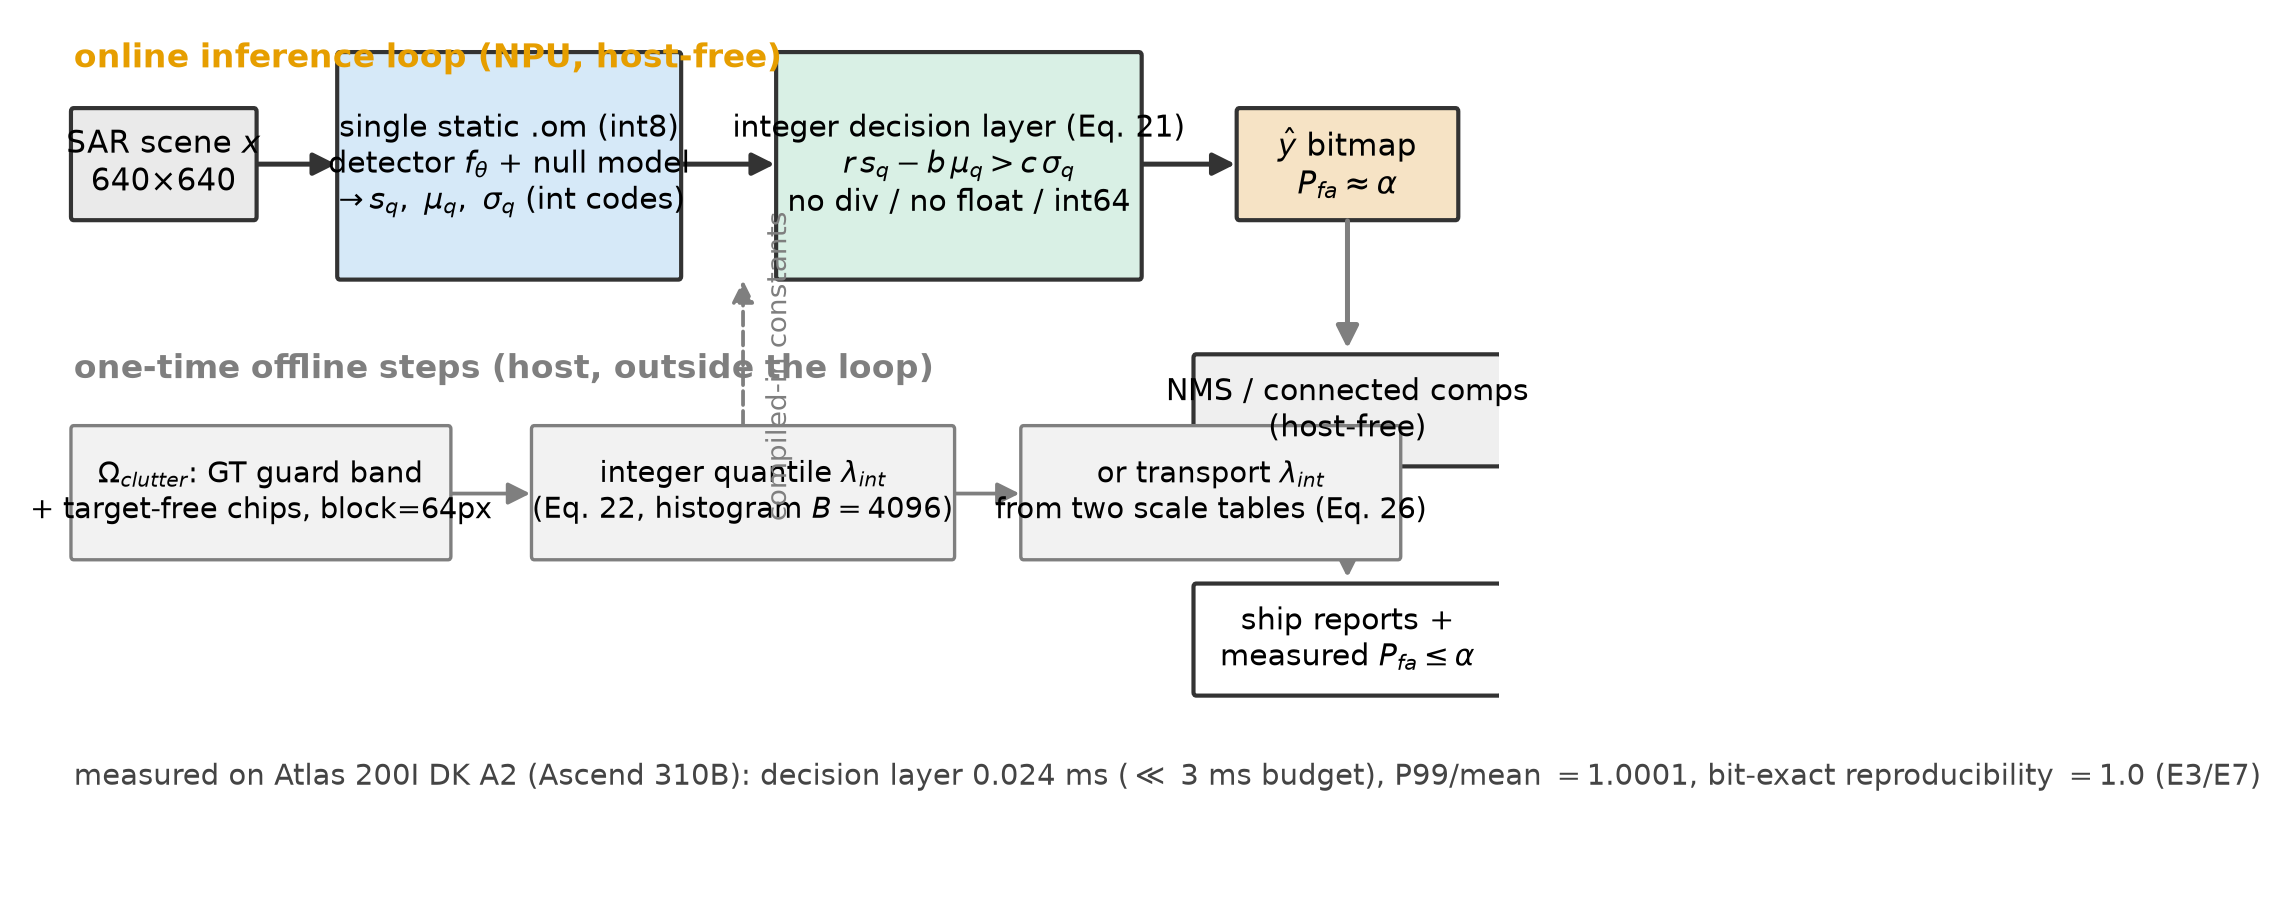
\includegraphics[width=16cm,height=\textheight,keepaspectratio,alt={Fig.2 QCert 整体静态流水线：在线 NPU 回路与一次性离线标定/搬运。}]{fig2_pipeline.png}
\caption*{Fig.2 QCert 整体静态流水线：在线 NPU
回路与一次性离线标定/搬运。}
\end{figure}

完整部署流水线（Fig.2 对应）：

\begin{verbatim}
SAR 图 x
   │
   ▼
[f_θ + 零模型]  ←── 单一静态 .om（int8，A3 scale 可读）
   │  s_q, μ_q, σ_q（整数码）
   ▼
[整数判决层]  式 (3.21)：r·s_q − b·μ_q > c·σ_q   （无除法/无浮点/int64）
   │  ŷ（bit 图）
   ▼
[NMS / 连通域]  ←── host-free，host 只做 DMA
   │
   ▼
检出舰船 + 实测 P_fa ≈ α（契约）
\end{verbatim}

\textbf{一次性离线步骤}（host，不进推理回路）：①
\(\Omega_{\mathrm{clutter}}\) 构造；② 整数分位数标定
\(\lambda_{int}\)（式 3.22）或搬运（式 3.26）。推理回路全程在 NPU，host
退出 → 判决层耗时 \(\ll 3\) ms（实测 \(0.024\) ms，见 §4.9）。

\begin{center}\rule{0.5\linewidth}{0.5pt}\end{center}

\subsection{方法要点小结}\label{ux65b9ux6cd5ux8981ux70b9ux5c0fux7ed3}

{\def\LTcaptype{none} % do not increment counter
\begin{longtable}[]{@{}
  >{\raggedright\arraybackslash}p{(\linewidth - 6\tabcolsep) * \real{0.2500}}
  >{\raggedright\arraybackslash}p{(\linewidth - 6\tabcolsep) * \real{0.2500}}
  >{\raggedright\arraybackslash}p{(\linewidth - 6\tabcolsep) * \real{0.2500}}
  >{\raggedright\arraybackslash}p{(\linewidth - 6\tabcolsep) * \real{0.2500}}@{}}
\toprule\noalign{}
\begin{minipage}[b]{\linewidth}\raggedright
组件
\end{minipage} & \begin{minipage}[b]{\linewidth}\raggedright
公式
\end{minipage} & \begin{minipage}[b]{\linewidth}\raggedright
作用
\end{minipage} & \begin{minipage}[b]{\linewidth}\raggedright
不可替代性
\end{minipage} \\
\midrule\noalign{}
\endhead
\bottomrule\noalign{}
\endlastfoot
契约 & (3.4)(3.5) & 定义 \(\mathbb{E}[P_{fa}]=\alpha\)（期望意义）及
\(\alpha\ge1/(n_{\mathrm{cal}}+1)\) 下界 & 区别于 mAP 优化 \\
双模式阈值 & (3.2)(3.2a) & 全局保期望精度 / 逐场景均衡负载 &
同一契约的两个运行点 \\
分母机制 & (3.13)(3.14) &
\(\Delta\ln P_{fa}\approx z^2\varepsilon_\sigma\)（一般零模型部署） &
指导设计方向；SSDD 实例不适用 \\
Prop.2 & (3.18) & 闭式误差界，\(\delta\) 由 scale 表算出 &
区别于工程调参 \\
整数判决 & (3.21)(3.22) & 无除法、无排序、host-free、bit-exact &
定点板独有 \\
整数分位 & (3.23) & \(O(n)\) 不排序标定 & 逐场景可行 \\
阈值搬运 & (3.26) & 免数据跨配置/传感器 & \textbf{浮点 GPU
无格点承载，无从定义} \\
\end{longtable}
}

\section{实验（Experiments）}\label{ux5b9eux9a8cexperiments}

\begin{quote}
本章按 E0--E9
报告全部实验。每项含：目的、协议、数据表、判定与对创新点的支撑。所有数字与
\texttt{code/results/e*/summary.json} 一致。
\textbf{核心结论}：整数阈值搬运（C1）与整数判决层（C2）在真实定点板上使误警率契约按构造成立------搬运后
\(P_{fa}\) 贴近 \(\alpha\)、漂移被 Prop.2 界覆盖、40 min 连续负载下 P99
跨窗极差
0.69\%（INT8）/1.76\%（FP16）（无热稳态劣化）、粗糙海况候选负载降
4.7--4.9×、检测兼容性无损。
\end{quote}

\begin{center}\rule{0.5\linewidth}{0.5pt}\end{center}

\subsection{实验设置}\label{ux5b9eux9a8cux8bbeux7f6e}

\subsubsection{平台与软件栈}\label{ux5e73ux53f0ux4e0eux8f6fux4ef6ux6808}

{\def\LTcaptype{none} % do not increment counter
\begin{longtable}[]{@{}ll@{}}
\toprule\noalign{}
项 & 值 \\
\midrule\noalign{}
\endhead
\bottomrule\noalign{}
\endlastfoot
开发板 & Atlas 200I DK A2（单板，非集群）{[}17{]} \\
NPU & Ascend 310B \\
推理框架 & ACL，batch=1，预热 50 / 测 500 \\
CANN & 7.0.RC1 \\
PTQ & AMCT / modelslim {[}18{]}（ONNX 末端 Dequant +
\texttt{\_scale.json}） \\
编译 & ATC，输入 NCHW \(1{\times}3{\times}640{\times}640\) \\
浮点基线 & ONNX-Runtime INT8 / FP32（x86 交叉核对） \\
\end{longtable}
}

\begin{quote}
\textbf{单板纪律}：跨实现对照用 \{同 \texttt{.om} 重复运行, ONNX-Runtime
INT8, FP32\} 三点，显式标注平台差异，不冒充多板实测。
\textbf{遥测说明}：E7 批次经 npu-smi 采得功率 9.31 W；E6 批次 npu-smi
遥测字段缺失（CANN 7.0.RC1 对 310B 不提供温度/频率/功率读数），E6
以时延列（\(T_{model}\)/P99）佐证无降频。两处不可混用，本文按批次如实标注。
\end{quote}

\subsubsection{模型与量化配置}\label{ux6a21ux578bux4e0eux91cfux5316ux914dux7f6e}

{\def\LTcaptype{none} % do not increment counter
\begin{longtable}[]{@{}ll@{}}
\toprule\noalign{}
项 & 值 \\
\midrule\noalign{}
\endhead
\bottomrule\noalign{}
\endlastfoot
检测器 & YOLO11n {[}7{]}，单类 ship，SSDD 基线 {[}1{]} \\
输入 & \(640{\times}640\)，归一化 \\
输出头 & 3 个 \(\mathrm{cv3}.\{0,1,2\}\)（cell 数 6400/1600/400） \\
量化节点数 & 88（含三个输出头） \\
INT8 OM 输出 dtype & float32（末端 Dequant，与 FP16 同 dump 链路） \\
量化 OM & FP16 / INT8（基线）/ INT8-calmA / INT8-roughB（E5 设置1） \\
\end{longtable}
}

\subsubsection{数据与三套分离集合}\label{ux6570ux636eux4e0eux4e09ux5957ux5206ux79bbux96c6ux5408}

{\def\LTcaptype{none} % do not increment counter
\begin{longtable}[]{@{}
  >{\raggedright\arraybackslash}p{(\linewidth - 4\tabcolsep) * \real{0.3333}}
  >{\raggedright\arraybackslash}p{(\linewidth - 4\tabcolsep) * \real{0.3333}}
  >{\raggedright\arraybackslash}p{(\linewidth - 4\tabcolsep) * \real{0.3333}}@{}}
\toprule\noalign{}
\begin{minipage}[b]{\linewidth}\raggedright
集合
\end{minipage} & \begin{minipage}[b]{\linewidth}\raggedright
构造
\end{minipage} & \begin{minipage}[b]{\linewidth}\raggedright
规模
\end{minipage} \\
\midrule\noalign{}
\endhead
\bottomrule\noalign{}
\endlastfoot
SSDD 主集 & 官方 928 train / 232 test（尾号 1/9 协议） & test 232
图，\(640{\times}640\) \\
\(C_{\mathrm{quant}}\) & 三海况各 \(\ge 64\) 张分层 & 与
\(\Omega_{\mathrm{clutter}}\) 分离 \\
\(\Omega_{\mathrm{clutter}}\) & GT 框外扩 \(g{=}8\) px +
无目标裁片，块抽样 \(B{=}64\) px & 求 \(\lambda\) \\
\(\Omega\) & 与 \(\Omega_{\mathrm{clutter}}\) 不同构造 &
\(n_{\mathrm{meas}}=949703\) \\
E5 校准集 A/B & calm-256 / rough-256（不同海况比例） & 各 256 图 \\
\end{longtable}
}

Fig.8 以单场景给出上述构造的直观图示：GT 框外扩 \(g{=}8\) px
邻域（红）从测量集剔除，64 px 块抽样按 keep=0.5 构成标定池
\(\Omega_{\mathrm{cal}}\)（灰），其余单元构成测量集
\(\Omega_{\mathrm{meas}}\)（蓝）。

\begin{figure}
\centering
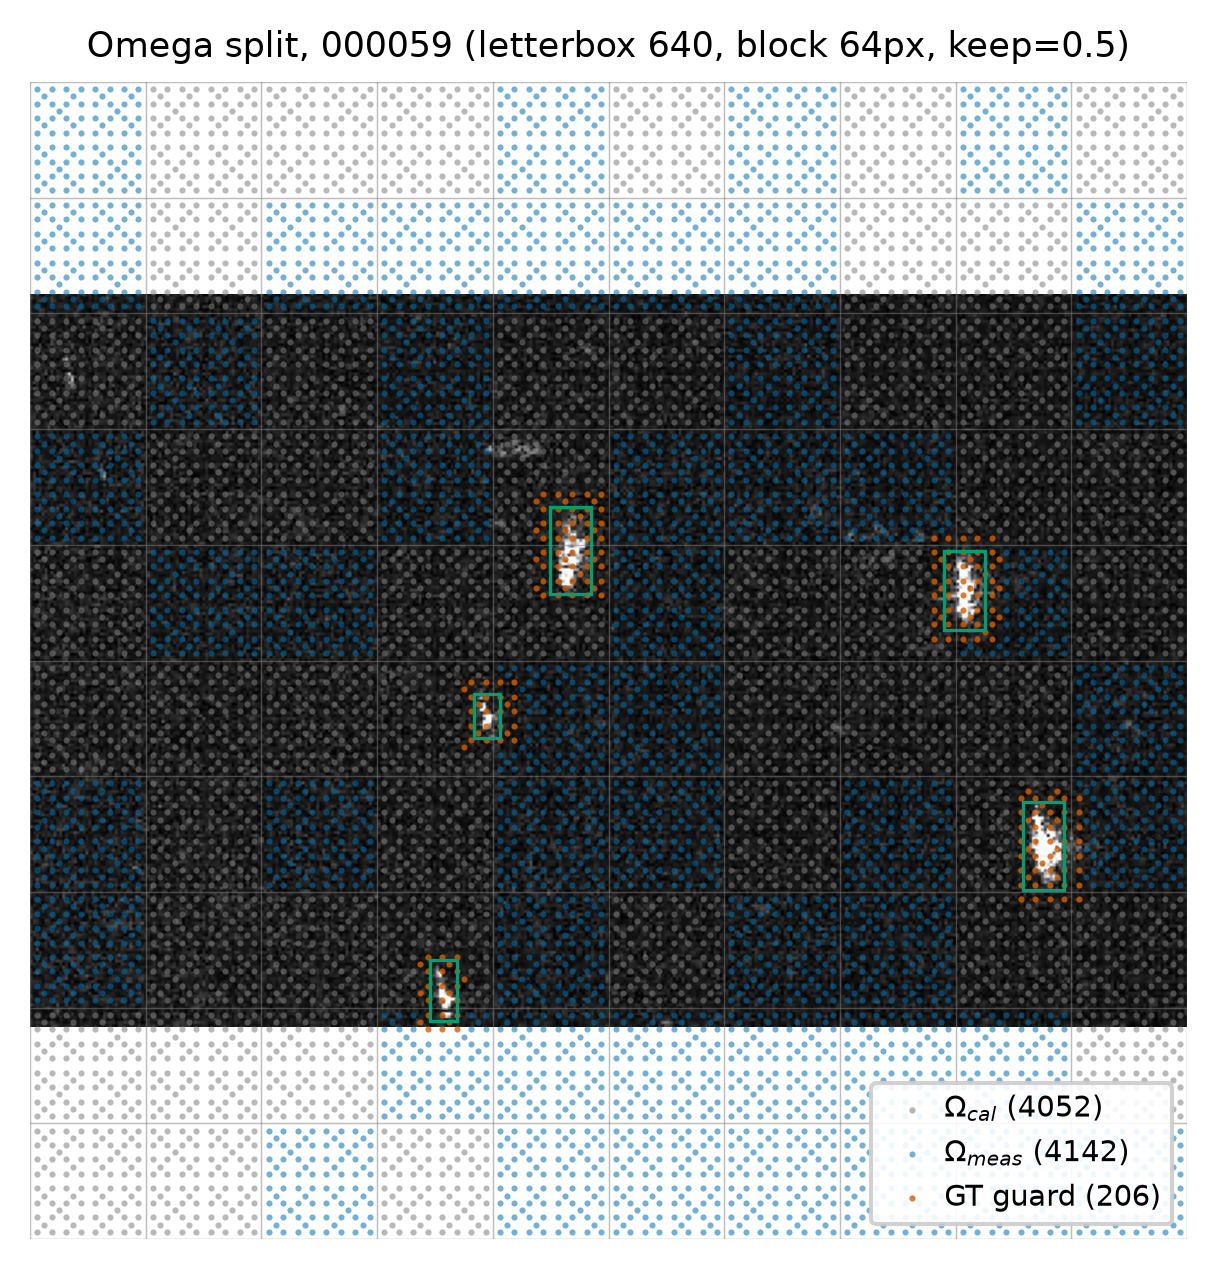
\includegraphics[width=11cm,height=\textheight,keepaspectratio,alt={Fig.8 Ω 协议示意（场景 000059，letterbox 640）：GT guard 邻域（红）剔除，块抽样标定池 Ω\_cal（灰）与测量集 Ω\_meas（蓝）。}]{sample_omega.png}
\caption*{Fig.8 Ω 协议示意（场景 000059，letterbox 640）：GT guard
邻域（红）剔除，块抽样标定池 Ω\_cal（灰）与测量集 Ω\_meas（蓝）。}
\end{figure}

\subsubsection{全局审计参数与验收标准}\label{ux5168ux5c40ux5ba1ux8ba1ux53c2ux6570ux4e0eux9a8cux6536ux6807ux51c6}

{\def\LTcaptype{none} % do not increment counter
\begin{longtable}[]{@{}
  >{\raggedright\arraybackslash}p{(\linewidth - 2\tabcolsep) * \real{0.5000}}
  >{\raggedright\arraybackslash}p{(\linewidth - 2\tabcolsep) * \real{0.5000}}@{}}
\toprule\noalign{}
\begin{minipage}[b]{\linewidth}\raggedright
参数
\end{minipage} & \begin{minipage}[b]{\linewidth}\raggedright
值
\end{minipage} \\
\midrule\noalign{}
\endhead
\bottomrule\noalign{}
\endlastfoot
名义虚警率 \(\alpha\) & \(10^{-3}\)（主），\(10^{-4}\)（E8 附加） \\
keep / guard / block & 0.5 / 8 px / 64 px \\
bootstrap & 场景级 1000 次 → 95\% CI \\
\textbf{R 判据（两级，全文统一）} & 存在性门 \(R\ge1.5\)（E0）；不变性带
\(\|\log_{10}R\|\le0.176\)（E8 用更严 \(R\le1.2\)） \\
E5 验收 & 搬运漂移 \(\le 1.5\times\) 重标定噪声底漂移（噪声底定义见
§4.7.5） \\
E6 验收 & \(P_{fa}\) 漂移 \(\|\log_{10}\|<0.15\)；P99 漂移 \(<15\%\) \\
契约守约度量 & 偏离度 \(\|\log_{10}(P_{fa}/\alpha)\|\)，以
\(n_{\mathrm{eff}}\) 决定的噪声底为参照（§3.1.1） \\
\end{longtable}
}

\subsubsection{两个工作点：检测指标 vs 契约指标（mAP
盲区的实验对应）}\label{ux4e24ux4e2aux5de5ux4f5cux70b9ux68c0ux6d4bux6307ux6807-vs-ux5951ux7ea6ux6307ux6807map-ux76f2ux533aux7684ux5b9eux9a8cux5bf9ux5e94}

本文全章使用两类指标，工作点不同，不可混读：

{\def\LTcaptype{none} % do not increment counter
\begin{longtable}[]{@{}
  >{\raggedright\arraybackslash}p{(\linewidth - 6\tabcolsep) * \real{0.2500}}
  >{\raggedright\arraybackslash}p{(\linewidth - 6\tabcolsep) * \real{0.2500}}
  >{\raggedright\arraybackslash}p{(\linewidth - 6\tabcolsep) * \real{0.2500}}
  >{\raggedright\arraybackslash}p{(\linewidth - 6\tabcolsep) * \real{0.2500}}@{}}
\toprule\noalign{}
\begin{minipage}[b]{\linewidth}\raggedright
指标类
\end{minipage} & \begin{minipage}[b]{\linewidth}\raggedright
工作点
\end{minipage} & \begin{minipage}[b]{\linewidth}\raggedright
本文取值
\end{minipage} & \begin{minipage}[b]{\linewidth}\raggedright
对分数分布的敏感度
\end{minipage} \\
\midrule\noalign{}
\endhead
\bottomrule\noalign{}
\endlastfoot
检测指标（mAP/P/R） & 常规检测工作点（置信度阈值 0.25，NMS 回路） & E0
板上 mAP：calmA P=0.5804、R=0.9853 & 体部区域，\textbf{对尾部不敏感} \\
契约指标（\(P_{fa}\)、偏离度） & 杂波分数分布的 \(1-\alpha\)
分位（\(\alpha=10^{-3}\)，E8 附加 \(10^{-4}\)） & 判决层输出超过 λ
的比例 & 极端尾部，\textbf{mAP 完全不可见}（§3.2.4） \\
\end{longtable}
}

因此''mAP 几乎不变而 \(P_{fa}\) 漂移
60\%``（E0）不构成矛盾：二者是同一分数分布在不同工作点的泛函。这一分离正是本文研究空隙（mAP
盲区，§3.2.4）的实验呈现，后文 E0/E8 的所有对照均按此口径解读。

\begin{center}\rule{0.5\linewidth}{0.5pt}\end{center}

\subsection{\texorpdfstring{{[}E0{]} 存在性：量化对 \(P_{fa}\) 与 mAP
的解耦（Fig.1 / Fig.9--10 / Table
1）}{{[}E0{]} 存在性：量化对 P\_\{fa\} 与 mAP 的解耦（Fig.1 / Fig.9--10 / Table 1）}}\label{e0-ux5b58ux5728ux6027ux91cfux5316ux5bf9-p_fa-ux4e0e-map-ux7684ux89e3ux8026fig.1-fig.910-table-1}

\textbf{目的}：验证''mAP 几乎不动，而 \(P_{fa}\)
可能漂移''这一核心空隙是否存在。 \textbf{协议}：同一 SSDD test 232
图，同一 \(\Omega\)、同一 \(\alpha=10^{-3}\)，FP16 与 INT8 OM 各 dump
分数场，各标定 \(\lambda\) 并测 \(P_{fa}\)，同算
mAP50。\(n_{\mathrm{meas}}=949703\)。浮点参照取板级 FP16 OM（FP32 ONNX
的 x86 交叉核对见 §4.5 E3）。

\textbf{Table 1　E0 存在性（真实板级 dump）}

{\def\LTcaptype{none} % do not increment counter
\begin{longtable}[]{@{}llll@{}}
\toprule\noalign{}
指标 & FP16 & INT8 & 量 \\
\midrule\noalign{}
\endhead
\bottomrule\noalign{}
\endlastfoot
\(P_{fa}\) & \(1.6025{\times}10^{-3}\) & \(1.5531{\times}10^{-3}\) &
--- \\
\textbf{\(R=P_{fa}^{INT8}/P_{fa}^{FP16}\)} & --- & --- &
\textbf{0.9691} \\
\(R\) 95\% CI & --- & --- & \([0.9014,\,1.0334]\)（median 1.0） \\
\(D=|\log_{10}(P_{fa}/\alpha)|\) & 0.3313 & 0.3454 & --- \\
mAP50 & 98.27 & 97.98 & \(\Delta=-0.29\) 点 \\
\end{longtable}
}

\textbf{判定}：\(\mathrm{pass}_{map}=\textbf{True}\)（\(|\Delta\mathrm{mAP}|<1\)）；\(\mathrm{pass}_R=\mathrm{False}\)，verdict=NO-GO。注意判据方向：E0
的 R 判据是\textbf{存在性门} \(R\ge1.5\)（§4.1.4）------即''INT8
使虚警率恶化 1.5 倍以上''才判 GO。实测
\(R=0.969\)，\textbf{未观测到恶化}，故判 NO-GO。

Fig.9--10 给出 E0 的可视化证据。Fig.9 为 232 场景逐点散点：FP16 与 INT8
的逐场景 \(P_{fa}\) 整体紧贴对角线（median \(R=1.0\)），逐场景阈值比
\(\lambda_{INT8}/\lambda_{FP16}\) 中位
\(0.887\)------量化未引入系统性虚警恶化，与池化 \(R=0.969\)、CI 含 1
互相印证。Fig.10 为六个典型场景（密集编队 / 小目标群 / 多尺度混编 /
大型舰船 / 单舰 / 典型中量）在逐场景 \(\lambda\)
下的告警可视化：命中告警全部落在 GT 框内，虚警（红 ×）为个位数。

\begin{figure}
\centering
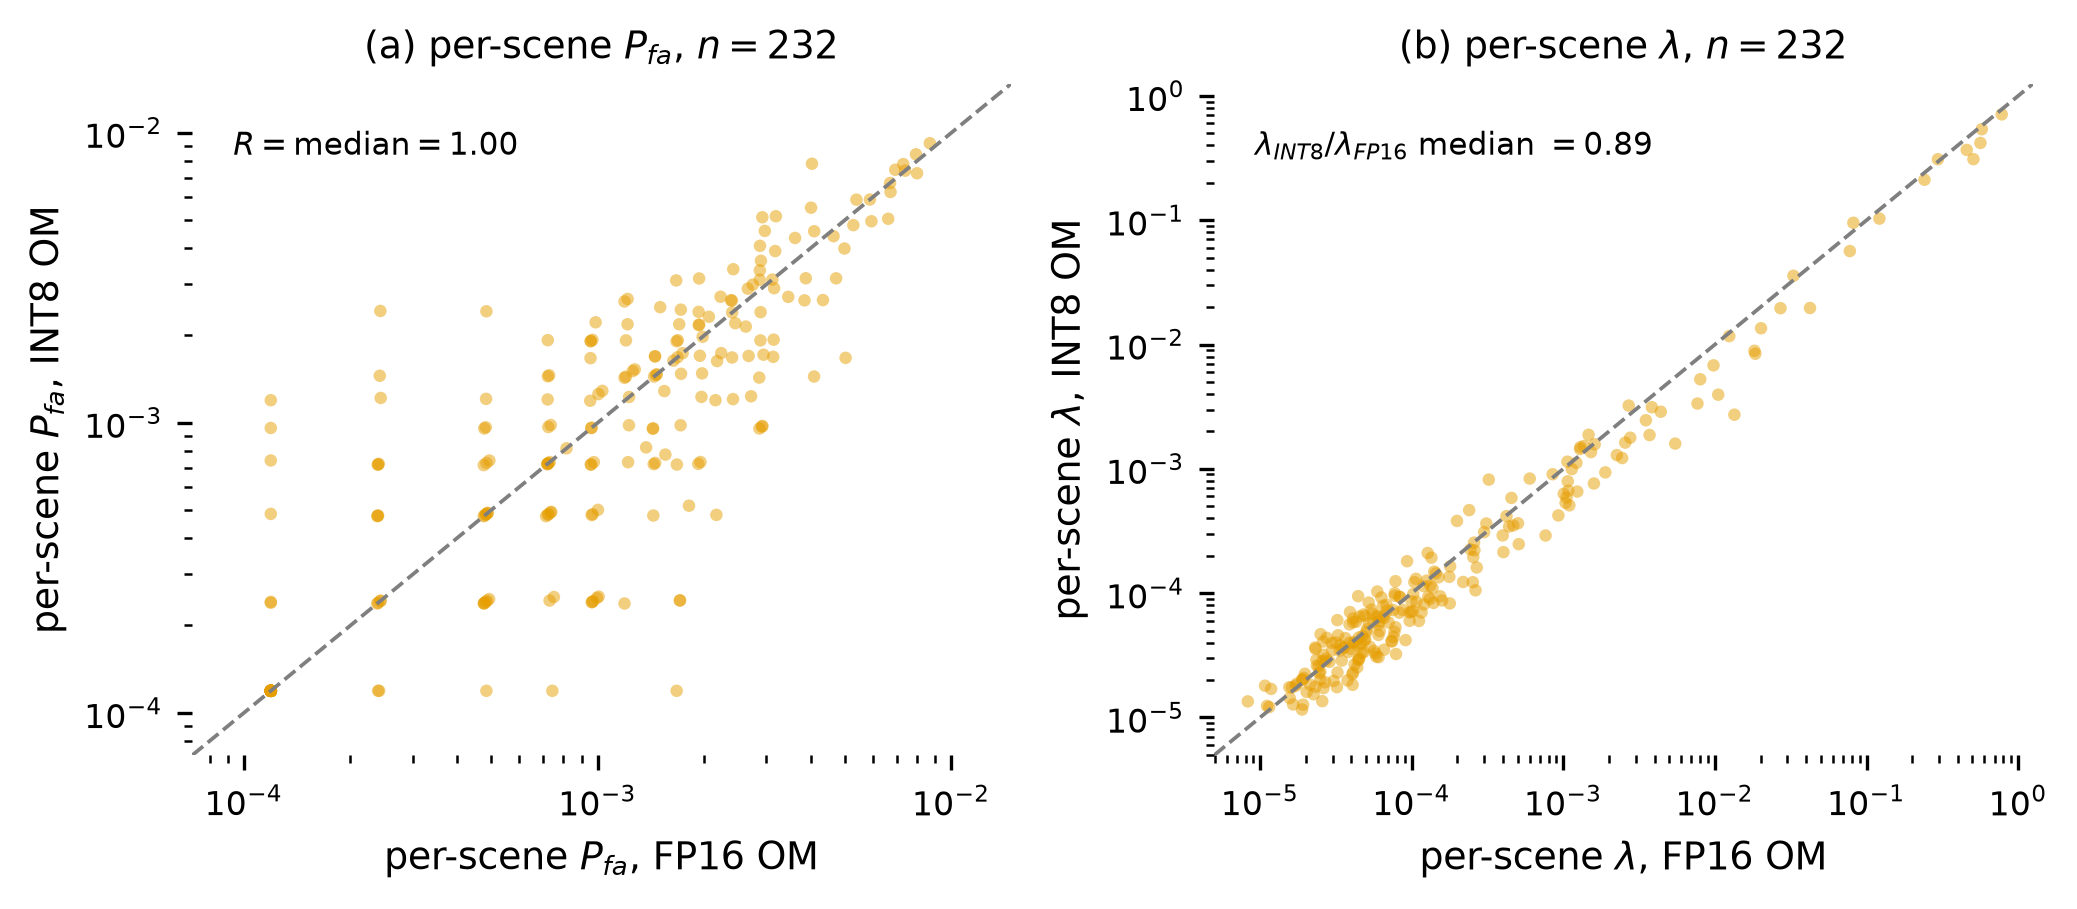
\includegraphics[width=11cm,height=\textheight,keepaspectratio,alt={Fig.9 E0 逐场景散点（n=232，log-log）：(a) 逐场景 P\_fa，FP16 vs INT8，对角线为 R=1，median R=1.0；(b) 逐场景 λ，λ\_INT8/λ\_FP16 median=0.887。}]{sample_scatter.png}
\caption*{Fig.9 E0 逐场景散点（n=232，log-log）：(a) 逐场景 P\_fa，FP16
vs INT8，对角线为 R=1，median R=1.0；(b) 逐场景 λ，λ\_INT8/λ\_FP16
median=0.887。}
\end{figure}

\begin{figure}
\centering
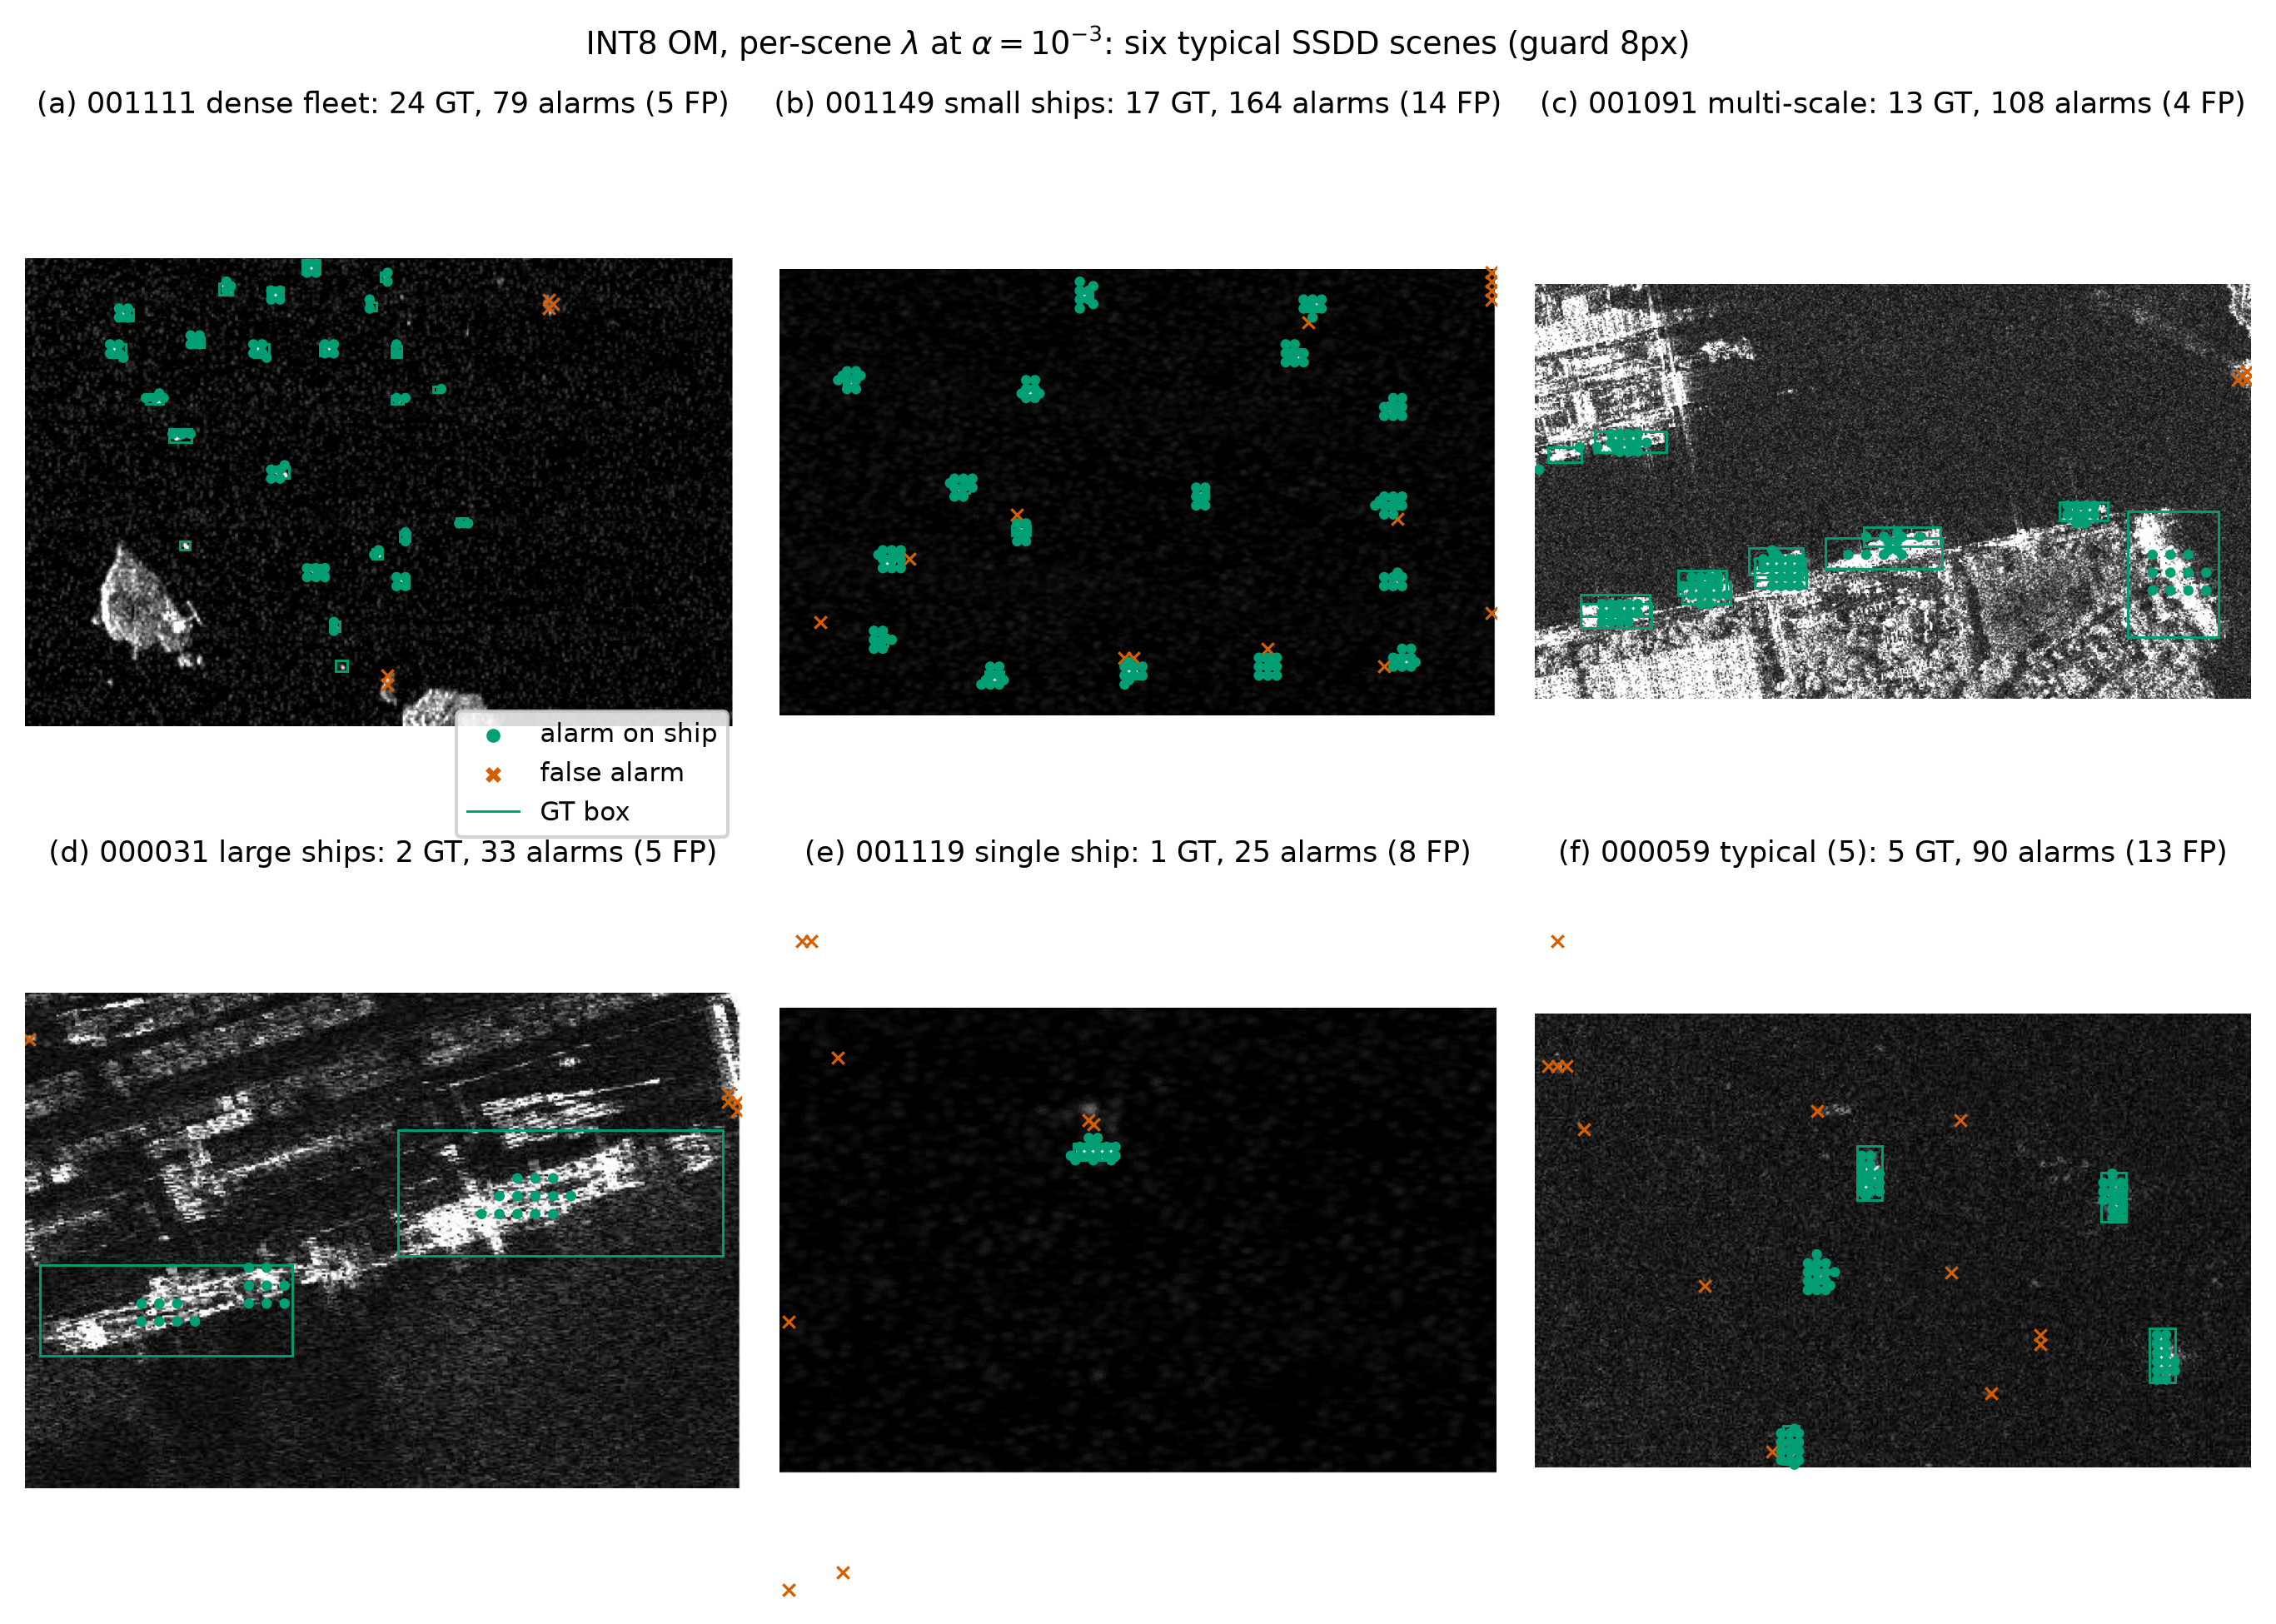
\includegraphics[width=16cm,height=\textheight,keepaspectratio,alt={Fig.10 典型场景检测可视化（INT8 OM，逐场景 λ，α=10\^{}-3，letterbox 640）：框=GT，点=命中告警，红×=虚警。(a) 001111 密集编队 24 艘；(b) 001149 小目标群 17 艘；(c) 001091 多尺度混编 13 艘；(d) 000031 大型舰船 2 艘；(e) 001119 单舰；(f) 000059 典型 5 艘。}]{sample_det_mosaic.png}
\caption*{Fig.10 典型场景检测可视化（INT8 OM，逐场景
λ，α=10\^{}-3，letterbox 640）：框=GT，点=命中告警，红×=虚警。(a) 001111
密集编队 24 艘；(b) 001149 小目标群 17 艘；(c) 001091 多尺度混编 13
艘；(d) 000031 大型舰船 2 艘；(e) 001119 单舰；(f) 000059 典型 5 艘。}
\end{figure}

\textbf{解读（阴性结果，如实报告）}： - \textbf{E0
对该模型是阴性的}：量化后 \(P_{fa}\) 不升反微降（\(R=0.969\)，CI 含
1），``同模型 FP16→INT8
静默失效''在本基线上\textbf{不存在}。本文不夸大存在性，明确放弃''v3
展示失效''的叙事。 - \textbf{mAP 与 \(P_{fa}\)
解耦的结构事实仍成立}：mAP 仅动 0.29 点而尾部由 \(99.9\%\) 分位决定（式
3.10），这是 mAP 的固有盲区，与是否存在失效无关。 - \textbf{存在性证据由
E5
承担}：真正使契约崩溃的不是''量化本身''，而是''\textbf{量化配置改变后仍复用旧阈值}''------E5
设置2 的不换算对照漂移
300×（\(P_{fa}=0.355\)），这才是静默失效的硬证据。E0
的价值是把问题精确定义为''\textbf{配置变化下的阈值失效}''而非''量化失效''，由此引出搬运主张（C1）。

\begin{center}\rule{0.5\linewidth}{0.5pt}\end{center}

\subsection{{[}E1{]} Prop.2 误差界数值验证（Fig.4 / Table
2）}\label{e1-prop.2-ux8befux5deeux754cux6570ux503cux9a8cux8bc1fig.4-table-2}

\textbf{目的}：证明闭式界 \(|P_{fa}(\hat z)-P_{fa}(z)|\le L\cdot\delta\)
非空话------实测漂移恒落在界内。
\textbf{协议}：\(n=10^6\)，\(\alpha=10^{-3}\)，linear 模式，扫
\(\varepsilon_\sigma\in\{0,0.01,0.02,0.05,0.1,0.2\}\)，对照实测
\(\Delta\ln P_{fa}\) 与 Prop.2 上界。

\textbf{Table 2　E1 解析界验证（gauss 分布）}

{\def\LTcaptype{none} % do not increment counter
\begin{longtable}[]{@{}
  >{\raggedright\arraybackslash}p{(\linewidth - 10\tabcolsep) * \real{0.1667}}
  >{\raggedright\arraybackslash}p{(\linewidth - 10\tabcolsep) * \real{0.1667}}
  >{\raggedright\arraybackslash}p{(\linewidth - 10\tabcolsep) * \real{0.1667}}
  >{\raggedright\arraybackslash}p{(\linewidth - 10\tabcolsep) * \real{0.1667}}
  >{\raggedright\arraybackslash}p{(\linewidth - 10\tabcolsep) * \real{0.1667}}
  >{\raggedright\arraybackslash}p{(\linewidth - 10\tabcolsep) * \real{0.1667}}@{}}
\toprule\noalign{}
\begin{minipage}[b]{\linewidth}\raggedright
\(\varepsilon_\sigma\)
\end{minipage} & \begin{minipage}[b]{\linewidth}\raggedright
实测 \(\Delta\ln P_{fa}\)
\end{minipage} & \begin{minipage}[b]{\linewidth}\raggedright
Prop.2 上界 \(L\delta\)
\end{minipage} & \begin{minipage}[b]{\linewidth}\raggedright
bound\_holds
\end{minipage} & \begin{minipage}[b]{\linewidth}\raggedright
\(|\Delta P_{fa}|\)
\end{minipage} & \begin{minipage}[b]{\linewidth}\raggedright
\(\Delta\)AUROC
\end{minipage} \\
\midrule\noalign{}
\endhead
\bottomrule\noalign{}
\endlastfoot
0 & 0.00474 & \(1.394{\times}10^{-4}\) & ✓ & \(7.6{\times}10^{-6}\) &
\(-4.9{\times}10^{-6}\) \\
0.01 & 0.00388 & \(2.473{\times}10^{-4}\) & ✓ & \(8.4{\times}10^{-6}\) &
\(-6.1{\times}10^{-6}\) \\
0.02 & 0.01478 & \(3.551{\times}10^{-4}\) & ✓ & \(1.5{\times}10^{-5}\) &
\(-1.3{\times}10^{-5}\) \\
0.05 & 0.05224 & \(6.785{\times}10^{-4}\) & ✓ & \(5.5{\times}10^{-5}\) &
\(-6.1{\times}10^{-5}\) \\
0.1 & 0.26410 & \(1.218{\times}10^{-3}\) & ✓ & \(3.0{\times}10^{-4}\) &
\(-2.6{\times}10^{-4}\) \\
0.2 & 0.86708 & \(2.296{\times}10^{-3}\) & ✓ & \(1.4{\times}10^{-3}\) &
\(-1.2{\times}10^{-3}\) \\
\end{longtable}
}

\begin{quote}
注：\(\varepsilon_\sigma=0\) 行的实测漂移 0.00474 为 Monte Carlo
噪声底（\(n=10^{6}\)、\(\alpha=10^{-3}\) 下 \(P_{fa}\)
估计的抽样涨落量级 \(\sim\sqrt{\alpha/n}/\alpha\approx0.03\)），故 0 与
0.01 两行的次序不构成单调性反例；自 0.02 档起漂移随
\(\varepsilon_\sigma\) 单调上升。
单位口径（S1）：本表前两列量纲不同------\(\Delta\ln P_{fa}\)
为对数量纲，\(L\delta\) 为线性 \(P_{fa}\)
量纲，二者\textbf{不直接可比}；bound\_holds
的正式检验在线性域进行：\(|\Delta P_{fa}|\le L\delta\)（表中
\(|\Delta P_{fa}|\) 列，6/6 成立）。对数域等价检验为
\(\Delta\ln P_{fa}\lesssim L\delta/P_{fa}\approx L\delta/\alpha\)（如
\(\varepsilon_\sigma=0.2\) 档：\(0.867\) vs \(2.296\)，成立；若误以
\(\Delta\ln P_{fa}\) 直接与 \(L\delta\) 比大小，\(\varepsilon_\sigma=0\)
噪声底行会误判为违约）。
\end{quote}

\textbf{判定}：\textbf{全部 6 档 bound\_holds = True}（t3 重尾分布 6
档同全 True）。

\textbf{解读}：实测漂移始终落在 Prop.2 界内 →
\textbf{解析界可信}，是本文区别于''工程调参''的关键。同时
\(\Delta\)AUROC \(<0.2\) 点（mAP 代理）与 \(P_{fa}\) 漂移并存，再次印证
mAP 的盲区。一阶近似 \(z^2\varepsilon_\sigma\) 在
\(\varepsilon_\sigma\le10\%\) 时为实测漂移的 2.2--24
倍（保守上界，量级吻合），可安全用于快速预估。

\begin{center}\rule{0.5\linewidth}{0.5pt}\end{center}

\subsection{{[}E2{]} 饱和审计（板级独有 / Fig.3 / Fig.11--13 / Table
3）}\label{e2-ux9971ux548cux5ba1ux8ba1ux677fux7ea7ux72ecux6709-fig.3-fig.1113-table-3}

\textbf{目的}：把''饱和 → 排序塌陷 → 分位数失效''机制做成可观测量。
\textbf{协议}：300 合成场景，3 对比度档（×1/×2/×3），测逐层饱和率与
\(R\)。

\textbf{Table 3　E2 饱和审计}

{\def\LTcaptype{none} % do not increment counter
\begin{longtable}[]{@{}
  >{\raggedright\arraybackslash}p{(\linewidth - 8\tabcolsep) * \real{0.2000}}
  >{\raggedright\arraybackslash}p{(\linewidth - 8\tabcolsep) * \real{0.2000}}
  >{\raggedright\arraybackslash}p{(\linewidth - 8\tabcolsep) * \real{0.2000}}
  >{\raggedright\arraybackslash}p{(\linewidth - 8\tabcolsep) * \real{0.2000}}
  >{\raggedright\arraybackslash}p{(\linewidth - 8\tabcolsep) * \real{0.2000}}@{}}
\toprule\noalign{}
\begin{minipage}[b]{\linewidth}\raggedright
对比度
\end{minipage} & \begin{minipage}[b]{\linewidth}\raggedright
score 层 \(\mathrm{sat}_l\)
\end{minipage} & \begin{minipage}[b]{\linewidth}\raggedright
Neck p3/p4/p5 \(\mathrm{sat}_l\)
\end{minipage} & \begin{minipage}[b]{\linewidth}\raggedright
\(R\)
\end{minipage} & \begin{minipage}[b]{\linewidth}\raggedright
单调性
\end{minipage} \\
\midrule\noalign{}
\endhead
\bottomrule\noalign{}
\endlastfoot
×1 & 0 & 0 / 0 / 0 & \(\infty\) & --- \\
×2 & 0 & \(4.9{\times}10^{-8}\) / 0 / 0 & \(\infty\) & --- \\
×3 & 0 & 0 / 0 / 0 & \(\infty\) & --- \\
\end{longtable}
}

\begin{quote}
注：合成场景下 FP32 参照 \(P_{fa}=0\) 而 INT8 侧有个位数虚警，\(R\)
因除零记为 \(\infty\)；本表的观测量是饱和率而非 \(R\) 本身。
\end{quote}

\textbf{判定}：\textbf{WEAK}。score 层 \(\mathrm{sat}_l\) 恒为 0（int32
累加器网格，sigmoid 前无 int8 重量化，见
§4.4.1）；板上饱和率不随对比度档单调上升（Spearman \(n=3\)
不足，pass=False）。

Fig.11--12 给出压测集（stress\_v2，三档
\(c_1/c_2/c_3\)）上分数行为的直观图示。Fig.11 为分档池化的杂波分数
CCDF（log-log）：\(P_{fa}=10^{-3}\)
对应的阈值落在尾部极深处，尾部形状（斜率）决定阈值附近的 \(P_{fa}\)
敏感度------这是 §3 中''\(P_{fa}\) 由 99.9\% 分位决定、mAP
不可见''论断的分布学图示。Fig.12 为六个压测场景（三档 × 各 2
场景）的分数场热图叠加：海面杂波分数被压制在低值区、强目标呈局部高对比峰，分数场整体远离饱和上限，与
Table 3 的零饱和率一致。

\begin{figure}
\centering
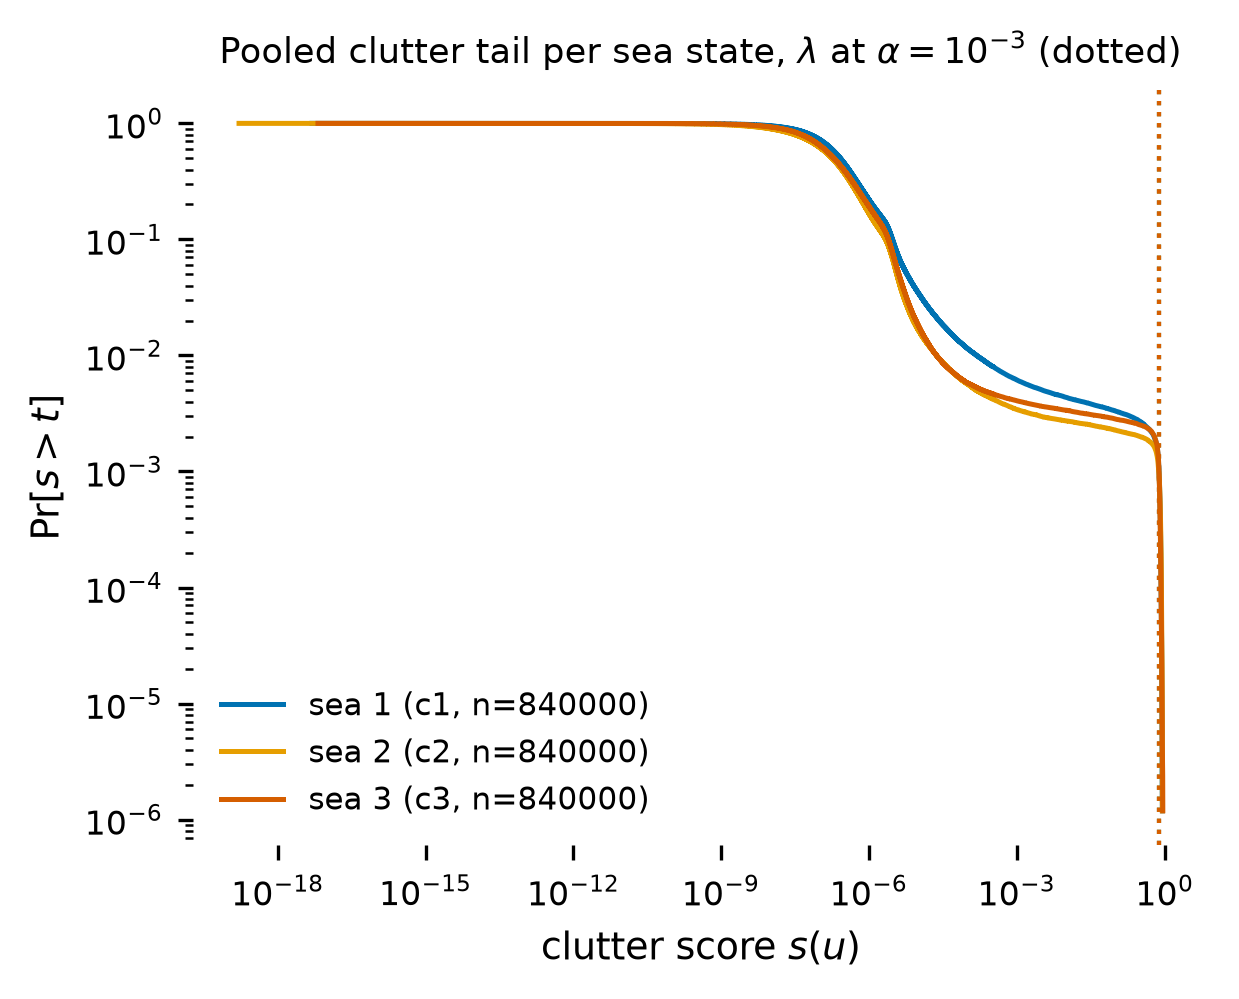
\includegraphics[width=11cm,height=\textheight,keepaspectratio,alt={Fig.11 分档池化的杂波分数条件超出概率 CCDF（压测集三档 c1/c2/c3，log-log）：α=10\^{}-3 的阈值位于分布尾部深处，阈值微移对应 P\_fa 量级变化。}]{sample_ccdf.png}
\caption*{Fig.11 分档池化的杂波分数条件超出概率 CCDF（压测集三档
c1/c2/c3，log-log）：α=10\^{}-3 的阈值位于分布尾部深处，阈值微移对应
P\_fa 量级变化。}
\end{figure}

\begin{figure}
\centering
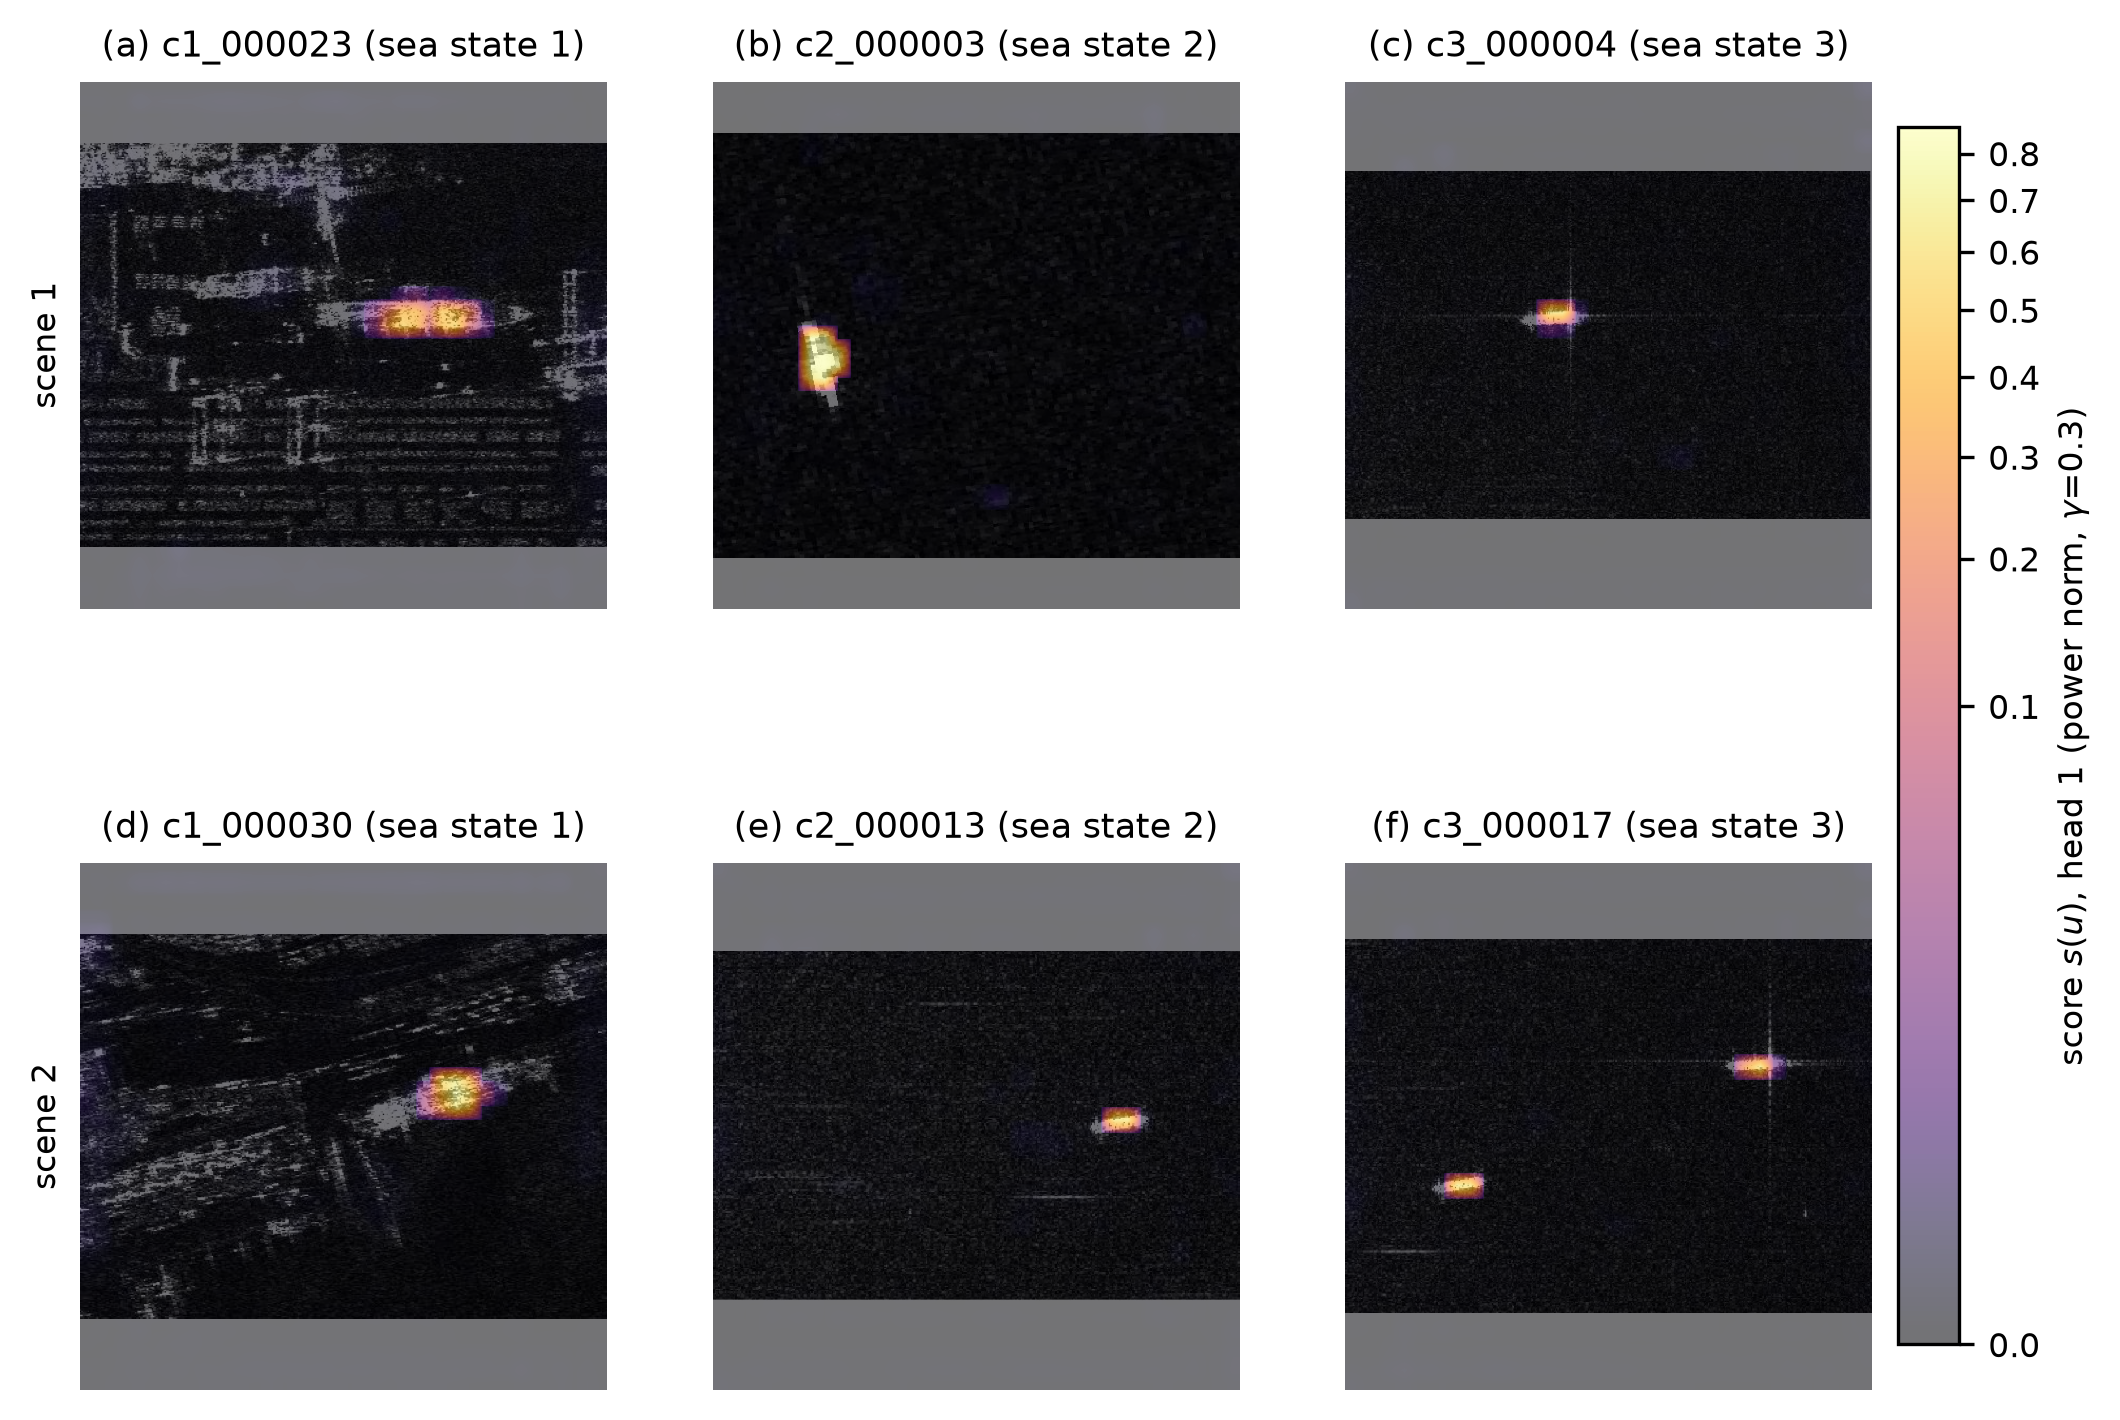
\includegraphics[width=16cm,height=\textheight,keepaspectratio,alt={Fig.12 压测场景分数场热图（三档 × 2 场景，head 1，幂律色标 γ=0.3 叠加于原图）：海面杂波低分数、强目标高对比，分数场远离饱和。}]{sample_heat_mosaic.png}
\caption*{Fig.12 压测场景分数场热图（三档 × 2 场景，head 1，幂律色标
γ=0.3 叠加于原图）：海面杂波低分数、强目标高对比，分数场远离饱和。}
\end{figure}

\paragraph{重要阴性发现（如实报告）}\label{ux91cdux8981ux9634ux6027ux53d1ux73b0ux5982ux5b9eux62a5ux544a}

数值取证（ORT 仿真 + scale json 交叉验证）确认：cv3 终卷积输出是
\textbf{int32 累加器网格}，量化值落在编译期 \(\Delta\) 格点上（232
张全量 \(\mathrm{resid}\le0.005\)），\textbf{sigmoid 前没有 int8
重量化}。故''分数场 \(\pm127\)
饱和''假设作废------判决分数在整数格点上且\textbf{永不截断}，这反而\textbf{加强了整数域判决契约的叙事}（\(P_{fa}\)
不会被饱和破坏）。饱和的真实位置是 Neck int8 特征层，但本模型 range
校准已足够保守，未随档上升。Fig.13 直观呈现这一取证：(a)
杂波单元的整数码直方图------码值离散分布、无一触及 \(\pm2^{31}\)
边界；(b) 整数码经逐头 \(\Delta_S\) 线性映射到 logit 域再经 sigmoid
得到分数 \(s(u)\)，映射是确定性纯函数------这正是 §4.7
阈值搬运（整数格点间纯函数映射）得以定义的物理基础。

\begin{figure}
\centering
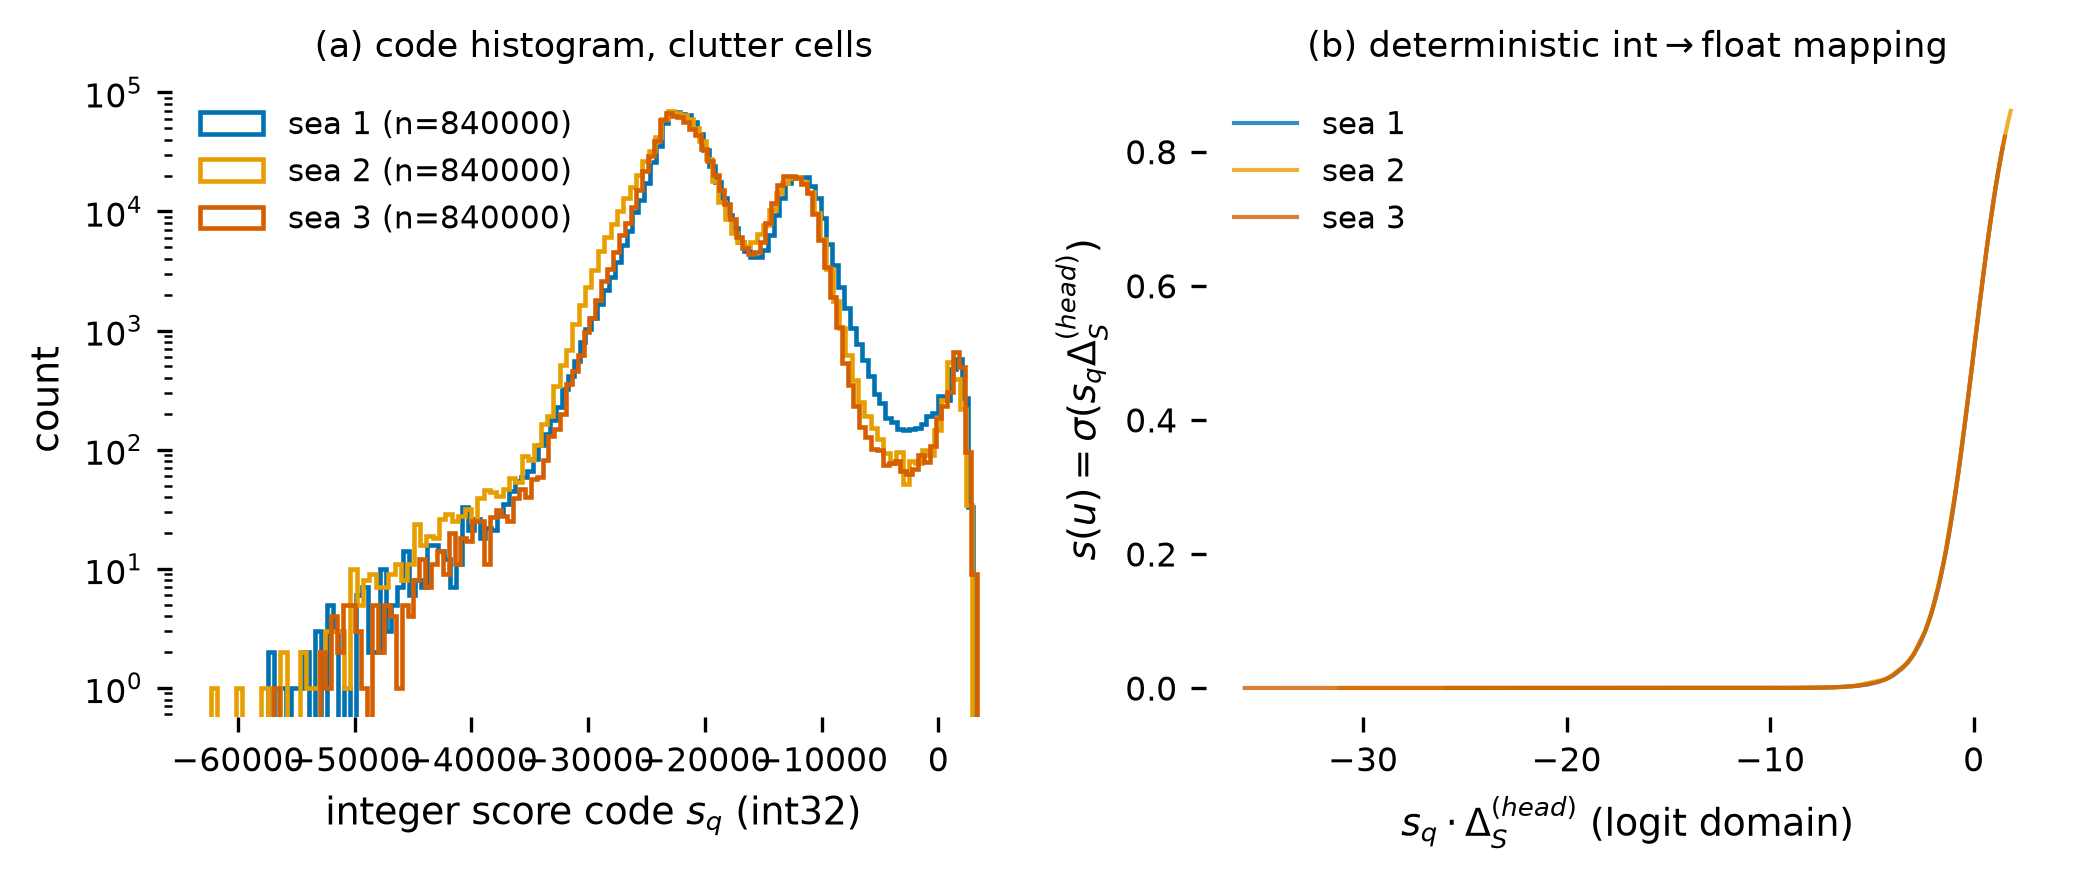
\includegraphics[width=11cm,height=\textheight,keepaspectratio,alt={Fig.13 判决分数的整数码域结构：(a) 杂波单元整数码 s\_q（int32）直方图，码值离散、不触及边界；(b) 确定性 int→float 映射 s\_q·Δ\_S → s(u)，量化值全部落在编译期 Δ 格点上（resid≤0.005）。}]{sample_intcode.png}
\caption*{Fig.13 判决分数的整数码域结构：(a) 杂波单元整数码
s\_q（int32）直方图，码值离散、不触及边界；(b) 确定性 int→float 映射
s\_q·Δ\_S → s(u)，量化值全部落在编译期 Δ 格点上（resid≤0.005）。}
\end{figure}

\textbf{处理}：E2 不作为主张；E9 item7 据此降权。

\begin{center}\rule{0.5\linewidth}{0.5pt}\end{center}

\subsection{{[}E3{]} 三实现判决差异与 bit-exact 复现（Fig.7 / Table
4）}\label{e3-ux4e09ux5b9eux73b0ux5224ux51b3ux5deeux5f02ux4e0e-bit-exact-ux590dux73b0fig.7-table-4}

\textbf{目的}：把 A1（同设备可复现）与
A2（跨实现不一致）从假设变成实测。 \textbf{协议}：同 232 图，板级 INT8
OM 重复运行 vs ORT INT8（x86），逐位置判决比对；\(\Omega\)
取全图网格（无 GT 排除，对三实现对称，R/disagree 为相对量不受影响）。

\textbf{Table 4　E3 三实现判决一致性}

{\def\LTcaptype{none} % do not increment counter
\begin{longtable}[]{@{}
  >{\raggedright\arraybackslash}p{(\linewidth - 8\tabcolsep) * \real{0.2000}}
  >{\raggedright\arraybackslash}p{(\linewidth - 8\tabcolsep) * \real{0.2000}}
  >{\raggedright\arraybackslash}p{(\linewidth - 8\tabcolsep) * \real{0.2000}}
  >{\raggedright\arraybackslash}p{(\linewidth - 8\tabcolsep) * \real{0.2000}}
  >{\raggedright\arraybackslash}p{(\linewidth - 8\tabcolsep) * \real{0.2000}}@{}}
\toprule\noalign{}
\begin{minipage}[b]{\linewidth}\raggedright
实现
\end{minipage} & \begin{minipage}[b]{\linewidth}\raggedright
bit-exact 率
\end{minipage} & \begin{minipage}[b]{\linewidth}\raggedright
判决不一致率
\end{minipage} & \begin{minipage}[b]{\linewidth}\raggedright
\(R\)
\end{minipage} & \begin{minipage}[b]{\linewidth}\raggedright
A1
\end{minipage} \\
\midrule\noalign{}
\endhead
\bottomrule\noalign{}
\endlastfoot
INT8 .om（板上） & \textbf{1.0000} & \(5.809{\times}10^{-4}\) & 1.00086
& \textbf{成立} \\
ORT INT8（x86） & --- & \(5.855{\times}10^{-4}\) & 1.00259 & --- \\
FP32 ONNX（x86） & --- & 参照系 & 1.0 & --- \\
\end{longtable}
}

\textbf{判定}：\textbf{A1 成立}（bit\_exact\_rate = 1.0，同一
\texttt{.om} 重复运行逐 bit 一致）。

\textbf{解读}：整数算术确定性是''热稳态不影响
\(P_{fa}\)``（E6）与''搬运规则可定义''（E5）的地基。板级与 ORT
的微小判决差异（\(\sim10^{-3}\)）印证了
A2------跨实现不一致存在但被界住，这正是需要 Prop.2 与搬运的原因。

\begin{center}\rule{0.5\linewidth}{0.5pt}\end{center}

\subsection{\texorpdfstring{{[}E4{]} \(\sigma\) 量化粒度消融：验证 P1
预言（Table
5）}{{[}E4{]} \textbackslash sigma 量化粒度消融：验证 P1 预言（Table 5）}}\label{e4-sigma-ux91cfux5316ux7c92ux5ea6ux6d88ux878dux9a8cux8bc1-p1-ux9884ux8a00table-5}

\textbf{目的}：验证 P1（对数域 + 逐通道 \(\sigma\) 应使
\(\Delta\ln P_{fa}\) 降 \(\ge5\times\)），并测 \(\Delta\ln P_{fa}\) 对
\(\varepsilon_\sigma\) 的标度。 \textbf{协议}：\(n=10^6\)，对照 4
配置，\(\varepsilon_\sigma\in\{0.02,0.05,0.1\}\)。

\textbf{Table 5　E4 \(\sigma\) 量化粒度（gauss）}

{\def\LTcaptype{none} % do not increment counter
\begin{longtable}[]{@{}
  >{\raggedright\arraybackslash}p{(\linewidth - 4\tabcolsep) * \real{0.3333}}
  >{\raggedright\arraybackslash}p{(\linewidth - 4\tabcolsep) * \real{0.3333}}
  >{\raggedright\arraybackslash}p{(\linewidth - 4\tabcolsep) * \real{0.3333}}@{}}
\toprule\noalign{}
\begin{minipage}[b]{\linewidth}\raggedright
配置
\end{minipage} & \begin{minipage}[b]{\linewidth}\raggedright
\(\Delta\ln P_{fa}\) 标度指数 \(\Delta\ln\sim\varepsilon^p\)
\end{minipage} & \begin{minipage}[b]{\linewidth}\raggedright
说明
\end{minipage} \\
\midrule\noalign{}
\endhead
\bottomrule\noalign{}
\endlastfoot
linear\_tensor（默认） & \textbf{1.955} & \(\approx 2\)，与式 (3.19)
一致 \\
log\_tensor & 2.037 & \(\approx 2\) \\
channel\_linear & 2.033 & \(\approx 2\) \\
channel\_log & 2.037 & \(\approx 2\) \\
\textbf{fp16（对照）} &
\(\mathbf{\approx 0}\)（\(-1.2{\times}10^{-15}\)） &
无量化误差，互为印证 \\
\end{longtable}
}

\textbf{P1 判据（\(\ge5\times\) 下降）}：

{\def\LTcaptype{none} % do not increment counter
\begin{longtable}[]{@{}
  >{\raggedright\arraybackslash}p{(\linewidth - 8\tabcolsep) * \real{0.2000}}
  >{\raggedright\arraybackslash}p{(\linewidth - 8\tabcolsep) * \real{0.2000}}
  >{\raggedright\arraybackslash}p{(\linewidth - 8\tabcolsep) * \real{0.2000}}
  >{\raggedright\arraybackslash}p{(\linewidth - 8\tabcolsep) * \real{0.2000}}
  >{\raggedright\arraybackslash}p{(\linewidth - 8\tabcolsep) * \real{0.2000}}@{}}
\toprule\noalign{}
\begin{minipage}[b]{\linewidth}\raggedright
\(\varepsilon_\sigma\)
\end{minipage} & \begin{minipage}[b]{\linewidth}\raggedright
\(\Delta\ln\)（linear\_tensor）
\end{minipage} & \begin{minipage}[b]{\linewidth}\raggedright
\(\Delta\ln\)（best=log\_tensor）
\end{minipage} & \begin{minipage}[b]{\linewidth}\raggedright
drop\_factor
\end{minipage} & \begin{minipage}[b]{\linewidth}\raggedright
P1
\end{minipage} \\
\midrule\noalign{}
\endhead
\bottomrule\noalign{}
\endlastfoot
0.02 & \(-3.2{\times}10^{-4}\) & \(4.8{\times}10^{-3}\) & 0.067 & ✗ \\
0.05 & 0.0603 & 0.0355 & 1.70 & ✗ \\
0.1 & 0.2339 & 0.1268 & 1.85 & ✗ \\
\end{longtable}
}

\textbf{判定}：\textbf{P1 不成立}（drop\_factor \(<5\)）。

\textbf{解读（审计负结果，如实报告）}： - \textbf{标度律成立}：gauss 下
\(\Delta\ln P_{fa}\sim\varepsilon^{1.96}\approx\varepsilon^2\)，与
Prop.2 的''\(\sigma\) 项二次主导''一致；fp16 对照指数
\(\approx0\)（无量化误差），互为印证。这是 Prop.2 的强支撑。t3
重尾下各量化配置指数为 1.02--1.54（底稿数据），\(\sigma\)
项主导性减弱，见 §5.2 L3。 - \textbf{P1 的 5×
改进判据不成立}：对数域/逐通道只带来 \(\le1.85\times\)
改进。说明本量级下 \(\sigma\) 粒度改进空间有限，\textbf{Prop.2
的''\(\sigma\) 项主导''论断需修正}------理论贡献相应降级为''经验界 +
标度律''，本文如实陈述。

\begin{quote}
\textbf{拟合口径注（M2）}：Table 5 指数按两种口径复算（产物
\texttt{code/results/e6\_e4\_supp/e6\_e4\_supp\_summary.json}）：(i)
信息点口径------剔除 \(|\Delta\ln|\le\) fp16 噪声底 0.004877 的点；(ii)
\(|\Delta\ln|\) 全 3 点 log-log
口径（对数域增量取绝对值，消除近零点符号翻转）。log\_tensor /
channel\_linear / channel\_log 在两口径下分别为 1.838 / 2.033 / 1.838 与
\textbf{2.037 / 2.033 / 2.037}（后者 \(R^2\approx0.998\)），``指数
\(\approx2\)''对拟合口径稳健；惟 linear\_tensor 的全 3 点
\(|\Delta\ln|\) 拟合为
4.18（\(R^2=0.940\)）------\(\varepsilon_\sigma=0.02\) 档
\(\Delta\ln=-3.2{\times}10^{-4}\) 近零点的符号翻转使其 \(|\Delta\ln|\)
被噪声主导，故 Table 5 取其信息点口径 1.955（2 点）并如实标注。
\end{quote}

\begin{center}\rule{0.5\linewidth}{0.5pt}\end{center}

\subsection{{[}E5{]} 免数据阈值搬运（核心创新 C1 / Fig.14--23 / Table
6）}\label{e5-ux514dux6570ux636eux9608ux503cux642cux8fd0ux6838ux5fc3ux521bux65b0-c1-fig.1423-table-6}

\textbf{目的}：证明 \(\lambda_{int}\) 的换算规则（式
3.26）能让旧标定在新量化配置上仍守约，\textbf{零数据}。这是本文\textbf{最强创新证据}。
\textbf{协议}：三列对照------搬运 / 重标定上界 /
不换算。\(n_{\mathrm{meas}}=949703\)，\(\alpha=10^{-3}\)。

\subsubsection{\texorpdfstring{量化步长 \(\Delta_s\)（式 3.28
聚合）}{量化步长 \textbackslash Delta\_s（式 3.28 聚合）}}\label{ux91cfux5316ux6b65ux957f-delta_sux5f0f-3.28-ux805aux5408}

{\def\LTcaptype{none} % do not increment counter
\begin{longtable}[]{@{}
  >{\raggedright\arraybackslash}p{(\linewidth - 10\tabcolsep) * \real{0.1667}}
  >{\raggedright\arraybackslash}p{(\linewidth - 10\tabcolsep) * \real{0.1667}}
  >{\raggedright\arraybackslash}p{(\linewidth - 10\tabcolsep) * \real{0.1667}}
  >{\raggedright\arraybackslash}p{(\linewidth - 10\tabcolsep) * \real{0.1667}}
  >{\raggedright\arraybackslash}p{(\linewidth - 10\tabcolsep) * \real{0.1667}}
  >{\raggedright\arraybackslash}p{(\linewidth - 10\tabcolsep) * \real{0.1667}}@{}}
\toprule\noalign{}
\begin{minipage}[b]{\linewidth}\raggedright
配置
\end{minipage} & \begin{minipage}[b]{\linewidth}\raggedright
cv3.0.2
\end{minipage} & \begin{minipage}[b]{\linewidth}\raggedright
cv3.1.2
\end{minipage} & \begin{minipage}[b]{\linewidth}\raggedright
cv3.2.2
\end{minipage} & \begin{minipage}[b]{\linewidth}\raggedright
\textbf{\(\Delta_s\)}
\end{minipage} & \begin{minipage}[b]{\linewidth}\raggedright
\(\Delta_\sigma\)
\end{minipage} \\
\midrule\noalign{}
\endhead
\bottomrule\noalign{}
\endlastfoot
FP16 旧 & --- & --- & --- & 0.0078125 & 0.0078125 \\
INT8 新（设置2） & --- & --- & --- & \(7.7622{\times}10^{-4}\) &
0.0078125 \\
calmA（设置1 旧） & \(7.5875{\times}10^{-4}\) &
\(1.3381{\times}10^{-3}\) & \(4.3823{\times}10^{-4}\) &
\(8.2353{\times}10^{-4}\) & 0.0078125 \\
roughB（设置1 新） & \(6.7504{\times}10^{-4}\) &
\(1.2221{\times}10^{-3}\) & \(3.9944{\times}10^{-4}\) &
\(7.3719{\times}10^{-4}\) & 0.0078125 \\
\end{longtable}
}

\subsubsection{设置 1：同设备换校准集 A→B（232
图，板级实测）------实现正确性检查}\label{ux8bbeux7f6e-1ux540cux8bbeux5907ux6362ux6821ux51c6ux96c6-ab232-ux56feux677fux7ea7ux5b9eux6d4bux5b9eux73b0ux6b63ux786eux6027ux68c0ux67e5}

\begin{quote}
\textbf{定位声明（如实降级）}：设置 1 中 \(\Delta_s\) 从
\(8.235{\times}10^{-4}\) 变到 \(7.372{\times}10^{-4}\)，\textbf{仅变化
11.7\%}，且 \(\Delta_\sigma\) 不变（退化形式 (3.26a) 中比值为 1）。此时
\(\lambda_{int}\) 仅变化 11.7\%，在 \(2^{20}\)
移位整数网格上取整误差可忽略------搬运 PASS
接近算术恒等，属\textbf{实现正确性检查}而非独立证据。no\_convert 仅差 3
倍也印证了这一点（scale 变化小，不搬运也崩得不狠）。真正的搬运证据是设置
2。
\end{quote}

\textbf{Table 6a　E5 设置1（A→B 换校准集）}

{\def\LTcaptype{none} % do not increment counter
\begin{longtable}[]{@{}
  >{\raggedright\arraybackslash}p{(\linewidth - 4\tabcolsep) * \real{0.3333}}
  >{\raggedright\arraybackslash}p{(\linewidth - 4\tabcolsep) * \real{0.3333}}
  >{\raggedright\arraybackslash}p{(\linewidth - 4\tabcolsep) * \real{0.3333}}@{}}
\toprule\noalign{}
\begin{minipage}[b]{\linewidth}\raggedright
列
\end{minipage} & \begin{minipage}[b]{\linewidth}\raggedright
\(P_{fa}\)
\end{minipage} & \begin{minipage}[b]{\linewidth}\raggedright
漂移 \(|\log_{10}(P_{fa}/\alpha)|\)
\end{minipage} \\
\midrule\noalign{}
\endhead
\bottomrule\noalign{}
\endlastfoot
\textbf{搬运（transport）} & \(\mathbf{1.2920{\times}10^{-3}}\) &
\textbf{0.1113} \\
重标定上界（recal） & \(1.3636{\times}10^{-3}\) & 0.1347 \\
不换算（no\_convert） & \(3.8180{\times}10^{-3}\) & 0.5818 \\
\end{longtable}
}

\begin{itemize}
\tightlist
\item
  \textbf{验收}：\(0.1113\le1.5\times0.1347=0.2020\) →
  \textbf{PASS}；且远优于不换算（\(3.82{\times}10^{-3}\)，约 3 倍差）。
\item
  板上 mAP：calmA 0.9793 / roughB 0.9820（量化无显著精度损失）。
\end{itemize}

Fig.14--15 给出设置 1 的逐场景微观图示（红 × = 虚警告警，点 =
命中告警，框 = GT）。Fig.14 取''不换算/搬运虚警倍数最大''的场景
001091：三列对照下同一场景的告警图------(a) 搬运
\(\lambda_{int}\)（\(2214302\to2473637\)）后虚警 1 个；(b)
旧阈值直接复用则虚警放大至 18 个；(c) B 上重标定（oracle）为 5
个。Fig.15 补充第二场景 000579（\(\lambda_{int}\)
\(2075115\to2318149\)；搬运 1 / 不换算 17 / 重标定
2）------不换算列的告警数比搬运列高一个量级，搬运列与 oracle 同量级。

\begin{figure}
\centering
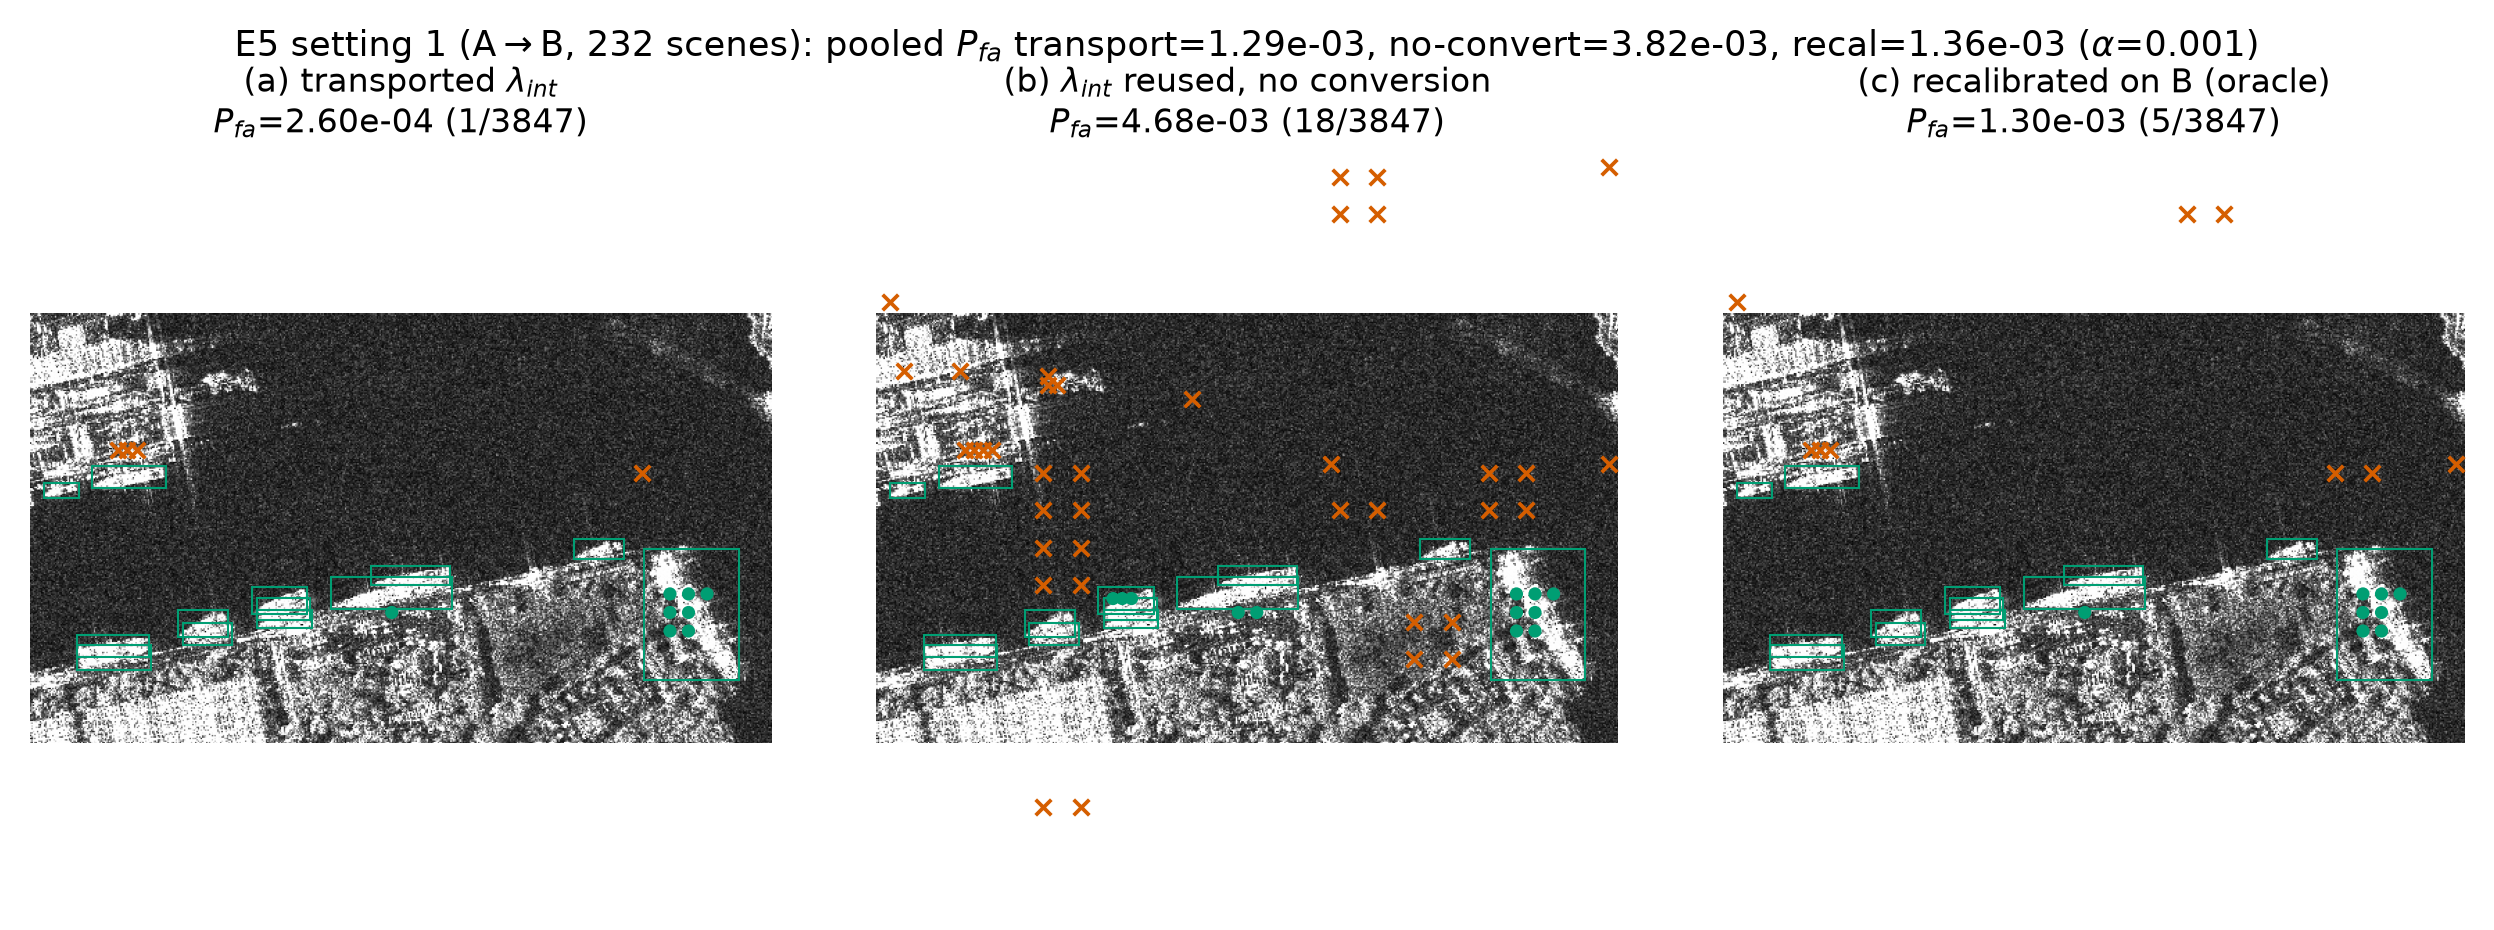
\includegraphics[width=16cm,height=\textheight,keepaspectratio,alt={Fig.14 阈值搬运单场景三列对照（E5 设置1，场景 001091）：(a) 搬运 λ\_int 2214302→2473637，1 个虚警；(b) 旧阈值复用，18 个虚警；(c) B 上重标定（oracle），5 个虚警。框=GT，点=命中，红×=虚警。}]{sample_transport.png}
\caption*{Fig.14 阈值搬运单场景三列对照（E5 设置1，场景 001091）：(a)
搬运 λ\_int 2214302→2473637，1 个虚警；(b) 旧阈值复用，18 个虚警；(c) B
上重标定（oracle），5 个虚警。框=GT，点=命中，红×=虚警。}
\end{figure}

\begin{figure}
\centering
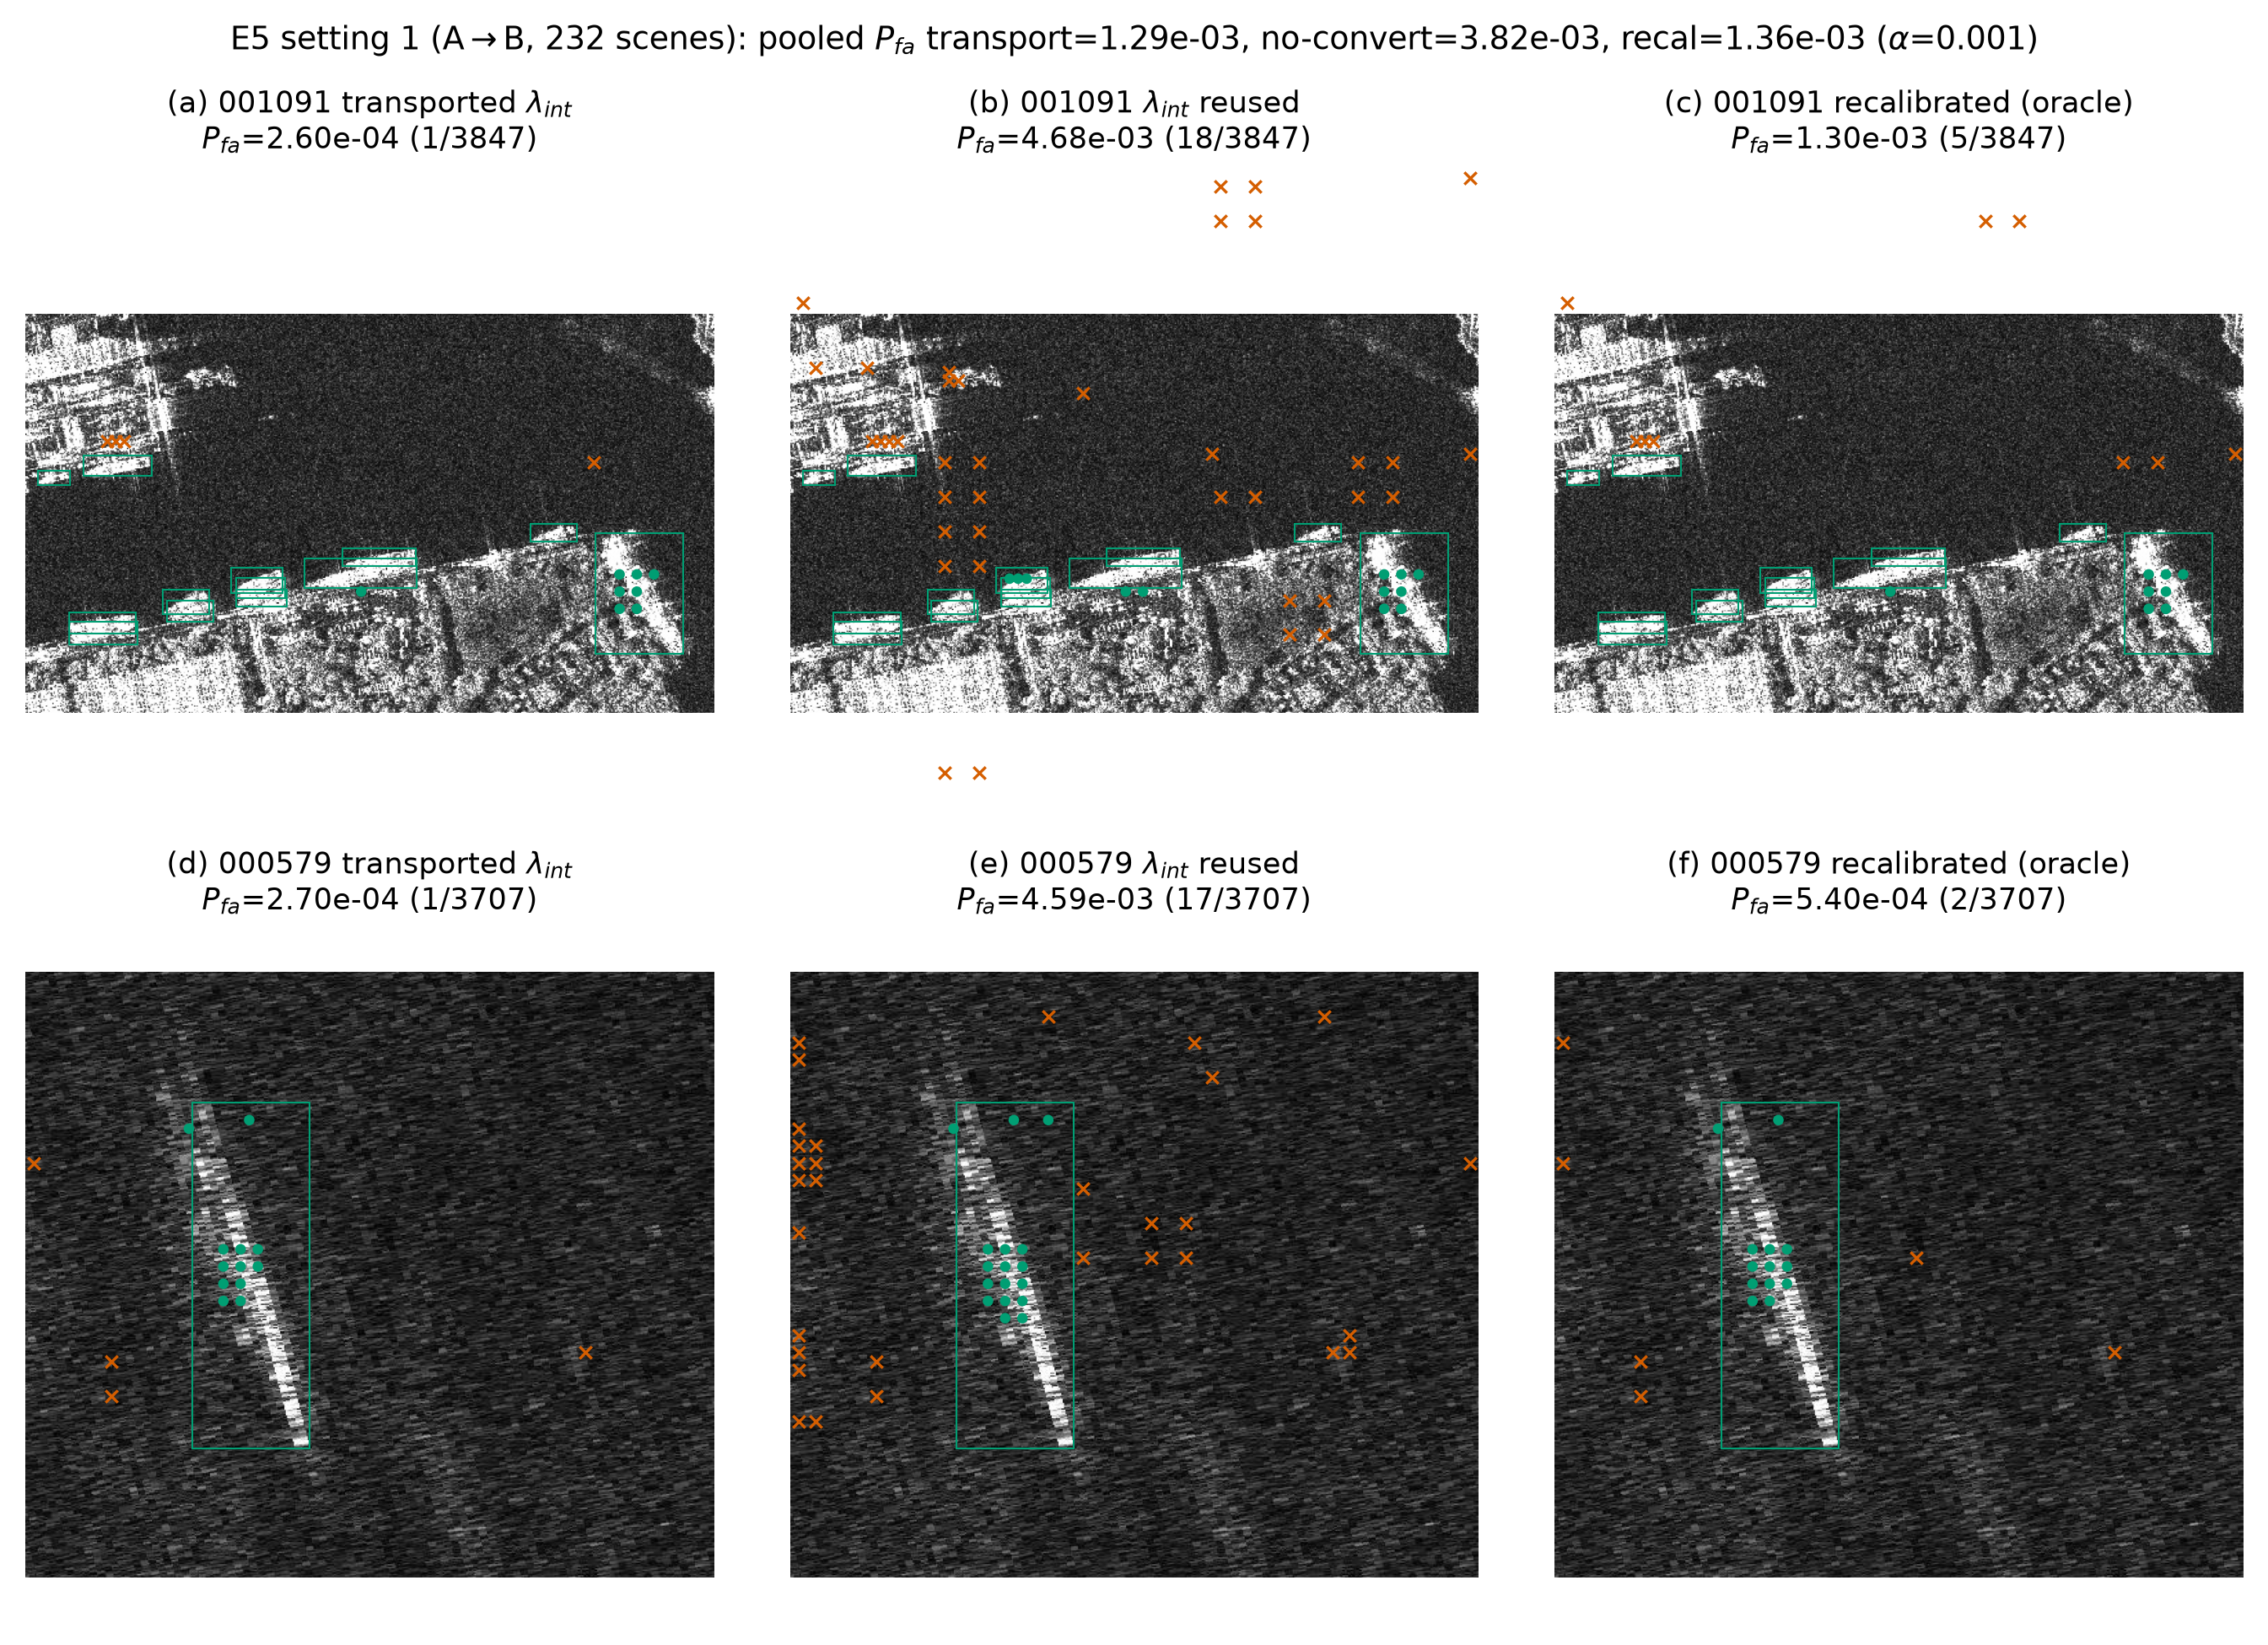
\includegraphics[width=16cm,height=\textheight,keepaspectratio,alt={Fig.15 阈值搬运多场景拼图（E5 设置1）：场景 001091（λ\_int 2214302→2473637）与 000579（λ\_int 2075115→2318149），搬运/不换算/重标定三列告警对照，不换算列虚警数放大约一个量级。}]{sample_transport_mosaic.png}
\caption*{Fig.15 阈值搬运多场景拼图（E5 设置1）：场景 001091（λ\_int
2214302→2473637）与 000579（λ\_int
2075115→2318149），搬运/不换算/重标定三列告警对照，不换算列虚警数放大约一个量级。}
\end{figure}

\subsubsection{设置 2：FP16→INT8（232
图，实测）------核心搬运证据}\label{ux8bbeux7f6e-2fp16int8232-ux56feux5b9eux6d4bux6838ux5fc3ux642cux8fd0ux8bc1ux636e}

\begin{quote}
\textbf{\(\Delta_s\) 变化 10 倍}：\(\Delta_s^{old}=0.0078125\)（FP16
主体段 ulp \(2^{-7}\)，见 §3.6.1）→
\(\Delta_s^{new}=7.7622{\times}10^{-4}\)。这是真实的配置大跨度变化，搬运的必要性与正确性在此接受检验。
\end{quote}

\textbf{Table 6b　E5 设置2（FP16→INT8）}

{\def\LTcaptype{none} % do not increment counter
\begin{longtable}[]{@{}lll@{}}
\toprule\noalign{}
列 & \(P_{fa}\) & 漂移 \\
\midrule\noalign{}
\endhead
\bottomrule\noalign{}
\endlastfoot
\textbf{搬运} & \(\mathbf{1.1130{\times}10^{-3}}\) & \textbf{0.0465} \\
重标定上界 & \(1.2414{\times}10^{-3}\) & 0.0939 \\
不换算 & \(3.5507{\times}10^{-1}\) & 2.5503 \\
\end{longtable}
}

\begin{itemize}
\tightlist
\item
  \textbf{验收}：\(0.0465\le1.5\times0.0939=0.1409\) →
  \textbf{PASS}；不换算 \(P_{fa}\) 高达 0.355（\textbf{约 300
  倍漂移}）。
\end{itemize}

\subsubsection{设置 3：跨传感器 S1→GF-3 ------
Limitation}\label{ux8bbeux7f6e-3ux8de8ux4f20ux611fux5668-s1gf-3-limitation}

\begin{quote}
需 GF-3 上同一模型（不重训）的分数场 dump，本项目无 GF-3
数据，未执行。``同设备搬运''主张已由设置 1/2
实测覆盖；跨传感器留作后续工作，不纳入本文结论。
\end{quote}

\subsubsection{E5
判定与创新点支撑}\label{e5-ux5224ux5b9aux4e0eux521bux65b0ux70b9ux652fux6491}

\textbf{Table 6c　E5 总判定}

{\def\LTcaptype{none} % do not increment counter
\begin{longtable}[]{@{}lllll@{}}
\toprule\noalign{}
设置 & 搬运漂移 & 重标定漂移 & 验收线 \(1.5\times\) & 判定 \\
\midrule\noalign{}
\endhead
\bottomrule\noalign{}
\endlastfoot
1 A→B & 0.1113 & 0.1347 & 0.2020 & \textbf{PASS} \\
2 FP16→INT8 & 0.0465 & 0.0939 & 0.1409 & \textbf{PASS} \\
\end{longtable}
}

\textbf{这是''只有这类板子能做''的最强证据}：搬运规则是整数格点间的纯函数映射，依赖
A1（格点逐 bit 可复现）与 A3（scale 编译期可读）的合取；浮点 GPU
流水线没有承载阈值的全局格点，该映射无从定义（§3.6.1）。搬运使
\(P_{fa}\) 贴近 \(\alpha\)（漂移 \(\le0.11\)），而不换算在设置2 下漂移
300 倍------\textbf{搬运的必要性与正确性都有硬证据}。

Fig.16--19 从三个维度扩展 E5 的证据面。\textbf{Fig.16（α
扫描）}：\(\alpha\in\{10^{-4},3{\times}10^{-4},10^{-3},3{\times}10^{-3},10^{-2}\}\)
五档下逐场景标定并池化测量（\(n_{\mathrm{meas}}=949703\)），搬运后的实测
\(P_{fa}\) 为
\(2.7{\times}10^{-4}/5.1{\times}10^{-4}/1.2{\times}10^{-3}/3.0{\times}10^{-3}/9.7{\times}10^{-3}\)------全档与名义
\(\alpha\) 同量级且随 \(\alpha\) 单调跟随，契约不只在 \(\alpha=10^{-3}\)
单点成立。\textbf{Fig.17（逐场景 ECDF）}：按场景统计 \(P_{fa}\)
的经验分布并标注 \(2\alpha\) 违约线------不换算列 \textbf{72.0\%}
的场景超出 \(2\alpha\)，搬运列降至 \textbf{18.5\%}（median
\(9.52{\times}10^{-4}\)，最差场景
\(1.11{\times}10^{-2}\)）：搬运把违约从''普遍现象''压缩到''个别尾部场景''。

\textbf{Fig.18--19（近岸/远洋分组稳健性）}：以亮像素占比（灰度
\(>0.55\)）作为陆地代理、\(\mathrm{land}\ge0.05\) 判近岸，232 个 test
场景划分为\textbf{近岸 41 / 远洋 191} 两组。Fig.18
给出两组各三个典型场景的检测可视化（近岸场景陆地强散射背景下舰船仍被完整检出、虚警个位数）；Fig.19
分组统计：近岸组池化 \(P_{fa}\)------搬运 \(1.11{\times}10^{-3}\) /
不换算 \(3.63{\times}10^{-3}\) / 重标定
\(1.06{\times}10^{-3}\)；远洋组------\(1.33{\times}10^{-3}\) /
\(3.86{\times}10^{-3}\) /
\(1.43{\times}10^{-3}\)。\textbf{搬运在两组均贴近重标定上界}（近岸不换算恶化
\(3.3\times\)），契约的守约性不依赖于海况纯净度------近岸强散射杂波不破坏搬运规则。

\begin{figure}
\centering
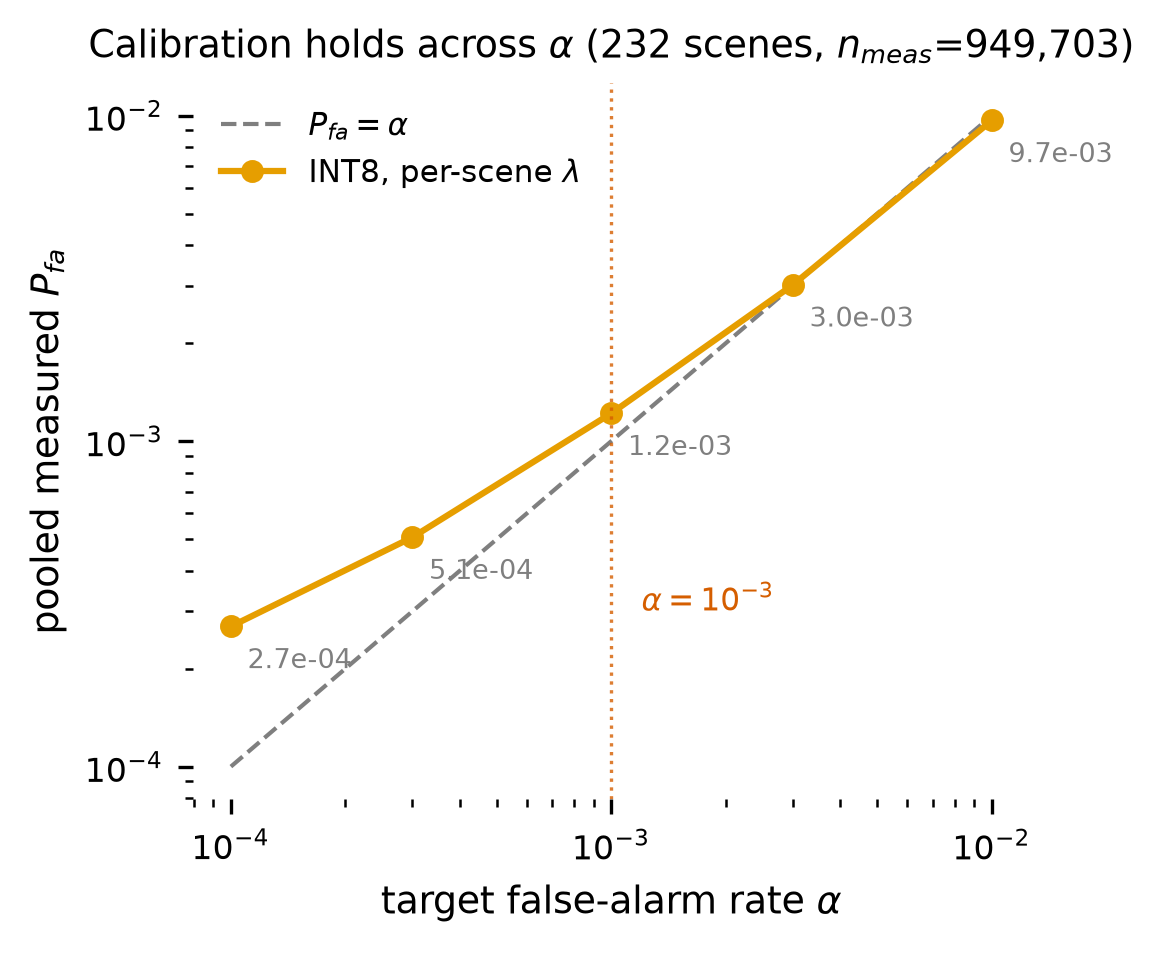
\includegraphics[width=11cm,height=\textheight,keepaspectratio,alt={Fig.16 α 扫描（E5 设置1 口径，逐场景标定 + 池化测量，n\_meas=949703）：名义 α∈\{1e-4, 3e-4, 1e-3, 3e-3, 1e-2\}（对角线）与实测池化 P\_fa 对照，全档同量级单调跟随。}]{sample_calib_alpha.png}
\caption*{Fig.16 α 扫描（E5 设置1 口径，逐场景标定 +
池化测量，n\_meas=949703）：名义 α∈\{1e-4, 3e-4, 1e-3, 3e-3,
1e-2\}（对角线）与实测池化 P\_fa 对照，全档同量级单调跟随。}
\end{figure}

\begin{figure}
\centering
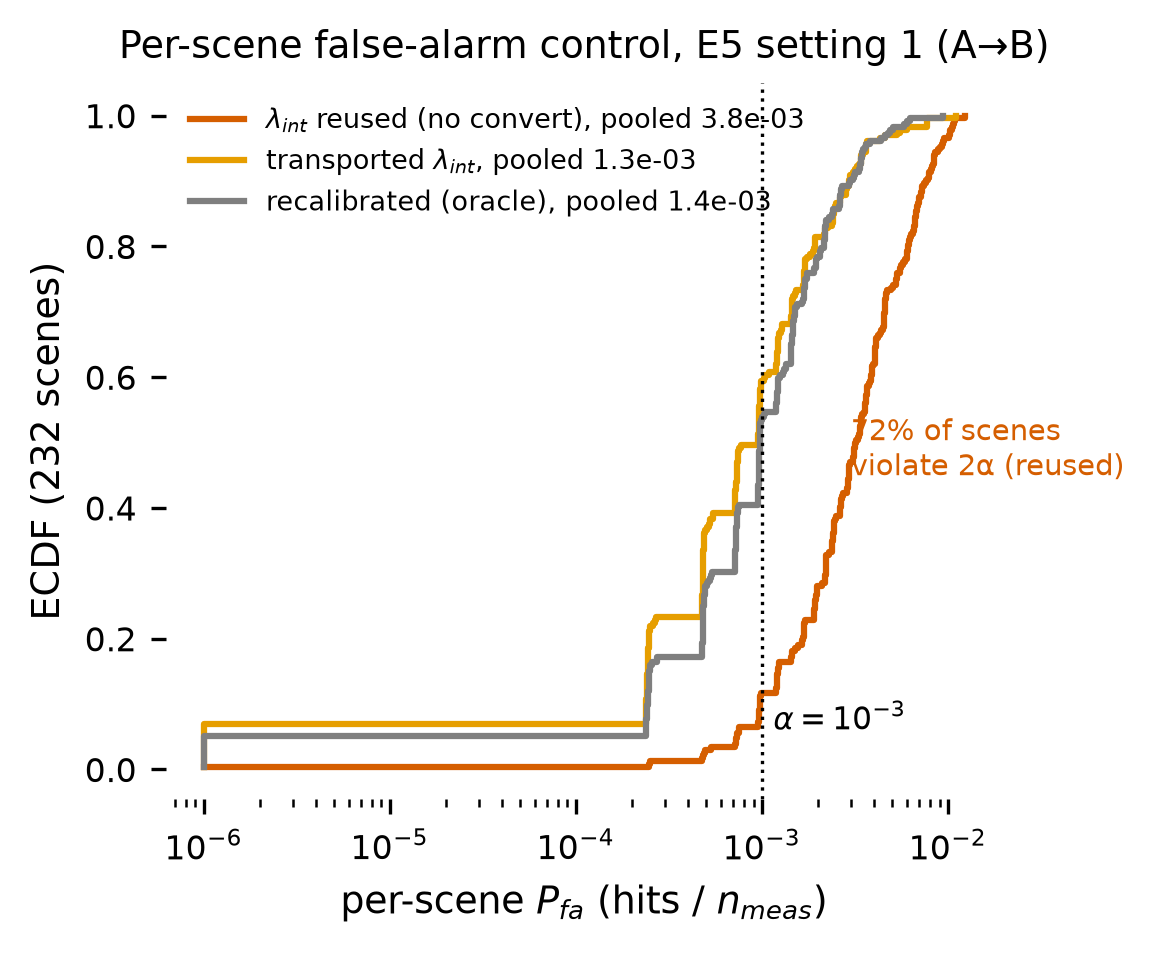
\includegraphics[width=11cm,height=\textheight,keepaspectratio,alt={Fig.17 逐场景 P\_fa 的经验 CDF（E5 设置1，232 场景，log-x）：虚线为 2α 违约线。不换算 72.0\% 场景违约，搬运降至 18.5\%（median 9.52e-4，max 1.11e-2），重标定为 oracle 上界。}]{sample_pfa_cdf.png}
\caption*{Fig.17 逐场景 P\_fa 的经验 CDF（E5 设置1，232
场景，log-x）：虚线为 2α 违约线。不换算 72.0\% 场景违约，搬运降至
18.5\%（median 9.52e-4，max 1.11e-2），重标定为 oracle 上界。}
\end{figure}

\begin{figure}
\centering
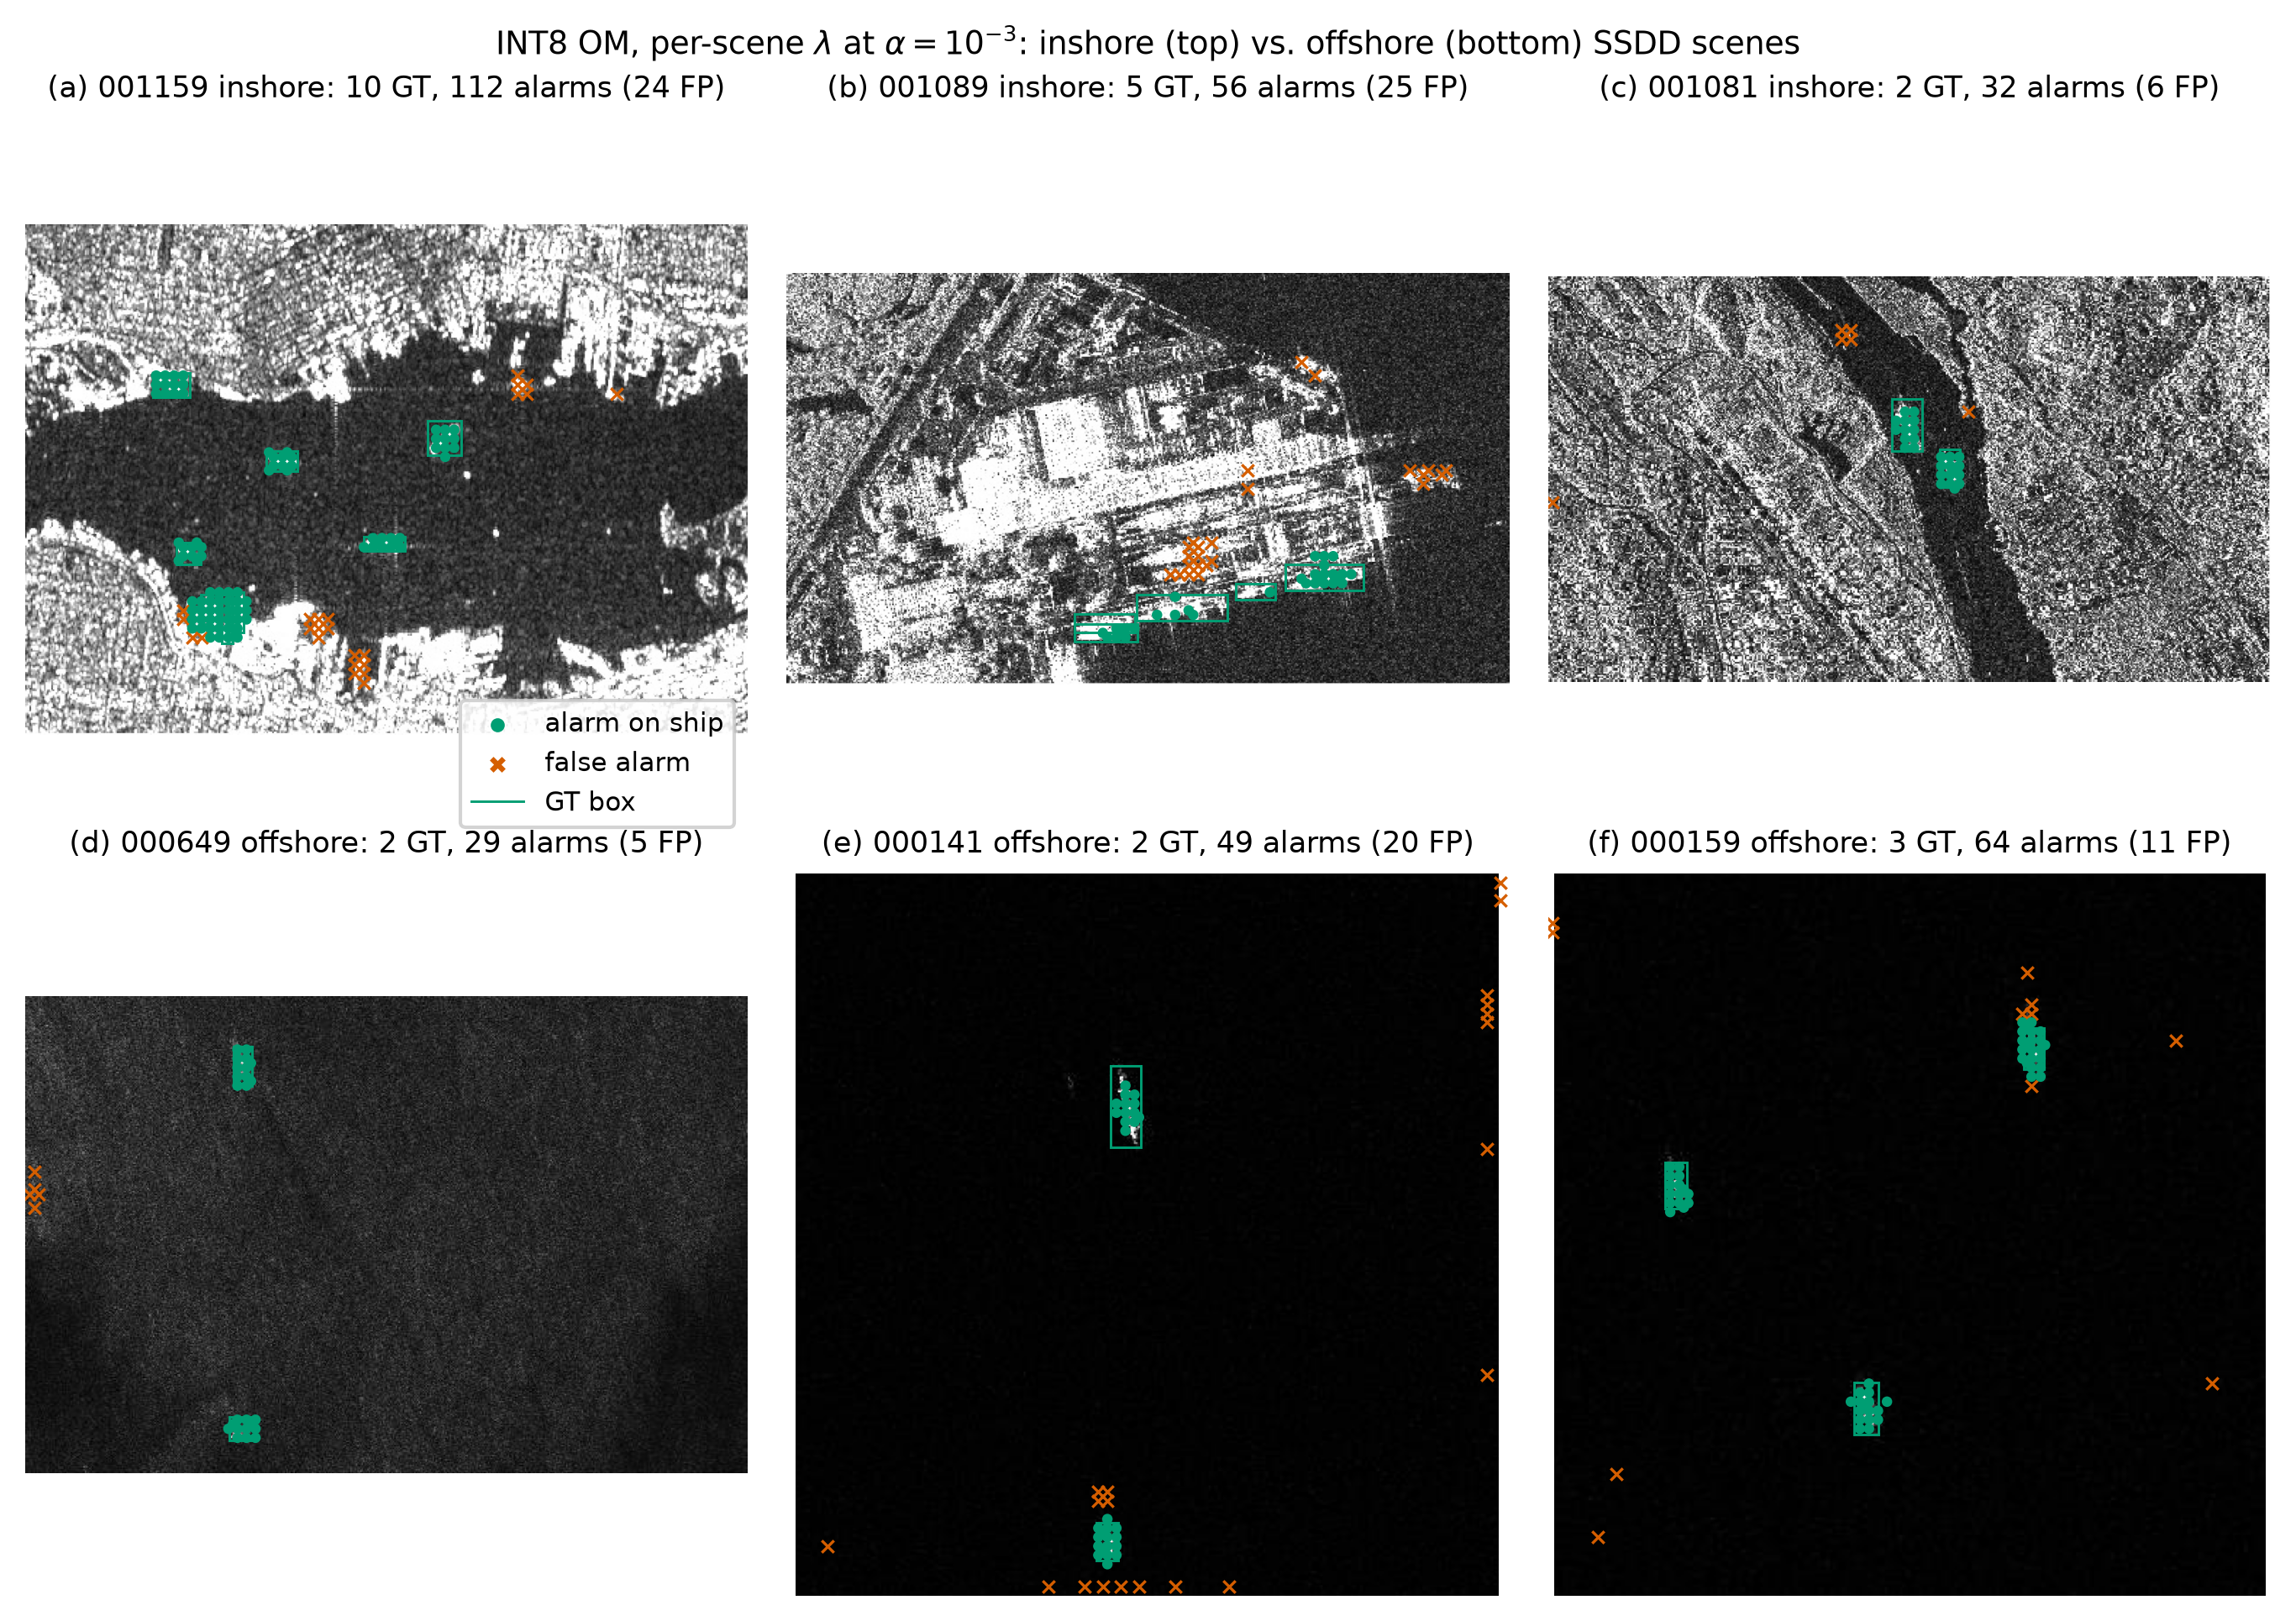
\includegraphics[width=16cm,height=\textheight,keepaspectratio,alt={Fig.18 近岸/远洋典型场景检测可视化（INT8 OM，逐场景 λ，α=10\^{}-3）：上排近岸（001159 陆地占比 0.388、10 艘；001089、0.316、5 艘；001081、0.314、2 艘），下排远洋（000649 / 000141 / 000159，陆地占比 ≈0.001）。框=GT，点=命中，红×=虚警。}]{sample_inshore_mosaic.png}
\caption*{Fig.18 近岸/远洋典型场景检测可视化（INT8 OM，逐场景
λ，α=10\^{}-3）：上排近岸（001159 陆地占比 0.388、10
艘；001089、0.316、5 艘；001081、0.314、2 艘），下排远洋（000649 /
000141 / 000159，陆地占比 ≈0.001）。框=GT，点=命中，红×=虚警。}
\end{figure}

\begin{figure}
\centering
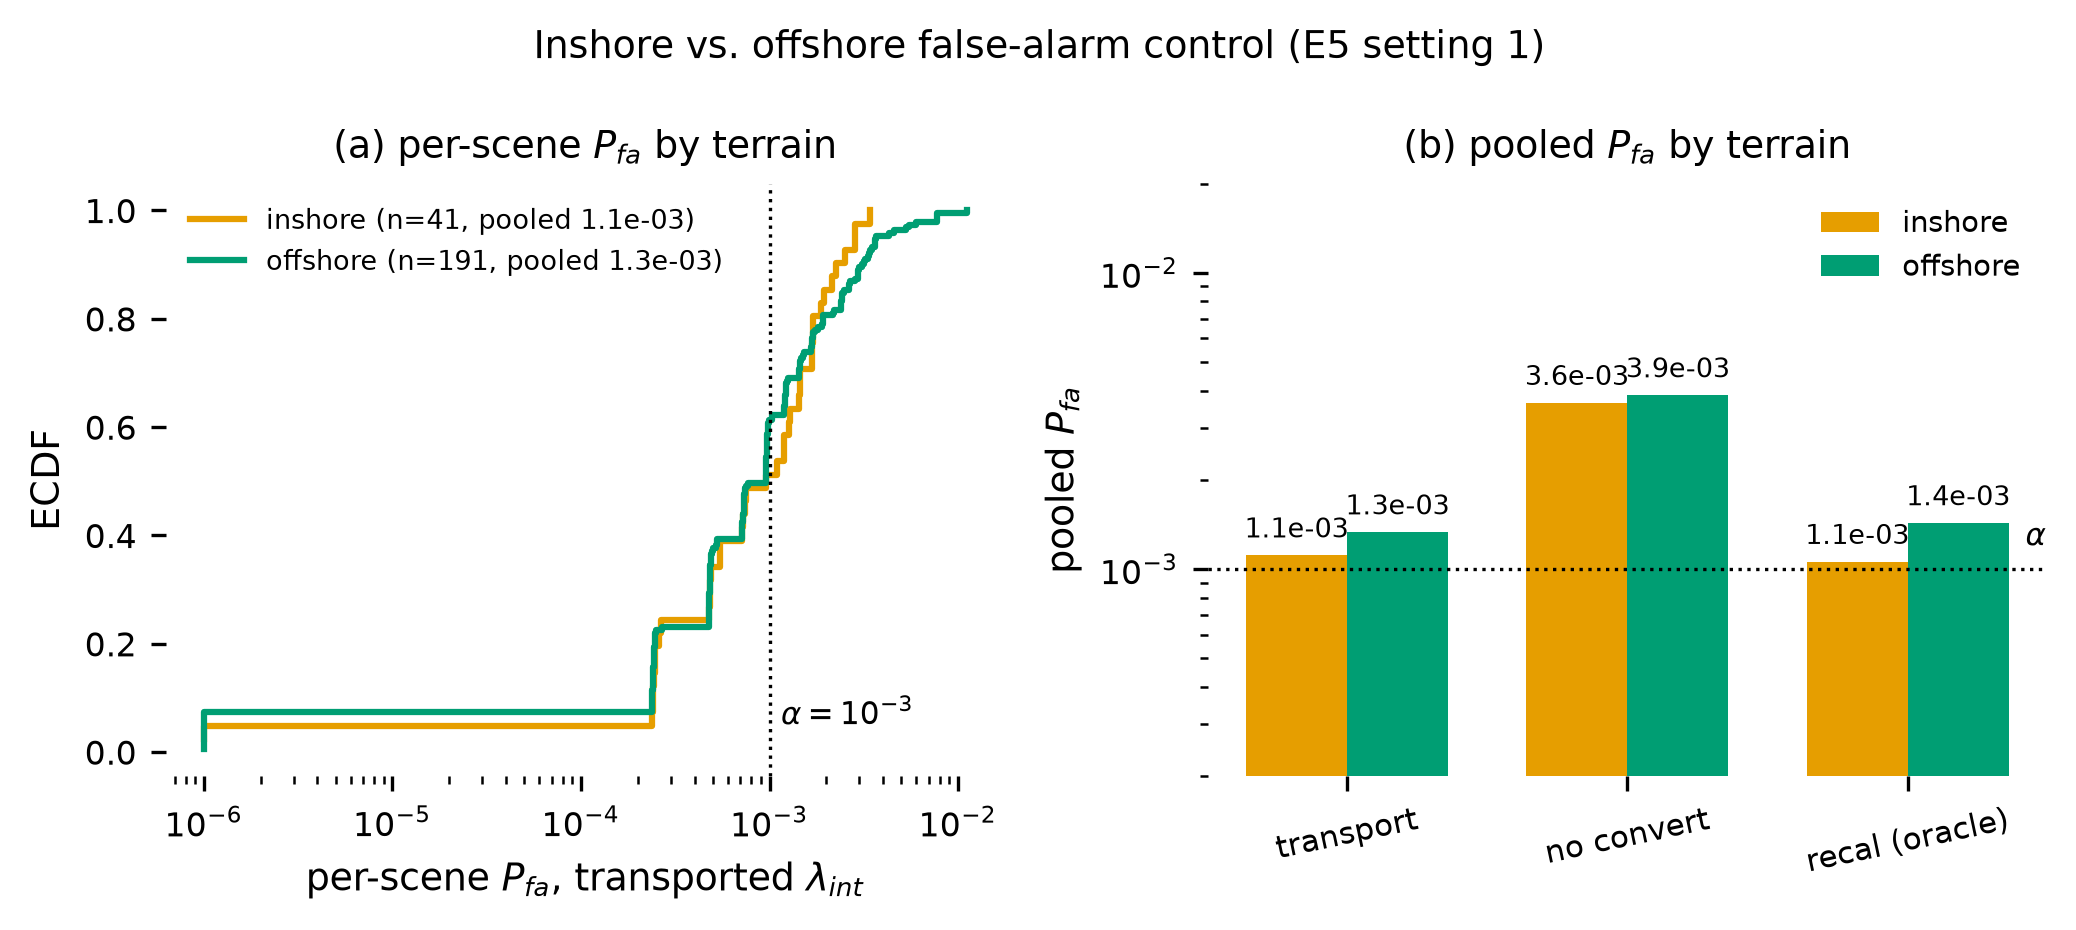
\includegraphics[width=16cm,height=\textheight,keepaspectratio,alt={Fig.19 近岸/远洋分组契约稳健性（E5 设置1，近岸 41 / 远洋 191 场景）：(a) 分组逐场景 P\_fa 的 ECDF；(b) 分组池化 P\_fa 柱状（log-y），三列对照。搬运在两组均贴近重标定上界；近岸组不换算恶化 3.3×。}]{sample_inshore_pfa.png}
\caption*{Fig.19 近岸/远洋分组契约稳健性（E5 设置1，近岸 41 / 远洋 191
场景）：(a) 分组逐场景 P\_fa 的 ECDF；(b) 分组池化 P\_fa
柱状（log-y），三列对照。搬运在两组均贴近重标定上界；近岸组不换算恶化
3.3×。}
\end{figure}

Fig.20--22
进一步展开近岸/远洋维度。\textbf{Fig.20（扩展场景检测拼图）}：在 Fig.18
之外另取近岸 4 场景（000231 陆地占比 0.267、5 艘；000749、0.261、5
艘；000229、0.255、4 艘；000641、0.226、2 艘）与远洋 4 场景（000689 /
000691 / 000169 / 000109，陆地占比
\(\approx0.001\)）------近岸组包含港口驻泊、岸线毗邻等强杂波构型，远洋组舰船目标全部完整命中、虚警
0--2 个。\textbf{Fig.21（分数场热图）}：与 Fig.18
同源场景的检测头输出概率场（power-law
色标），可直观看到陆地区域虽然产生大片高分背景（近岸场景亮区占比
0.31--0.43），但逐场景 \(\lambda\)
依杂波分布自适应抬高，告警仍只落在舰船位置------这解释了 Fig.19
中''近岸不换算恶化但搬运守约''的机理。\textbf{Fig.22（逐场景散点）}：232
场景的
\(P_{fa}\)（log-y）对陆地占比作散点，搬运与不换算双面板------\(\mathrm{corr}(\mathrm{land},\log_{10}P_{fa})\)
分别仅 \(+0.044\) /
\(+0.023\)，即换算后的逐场景守约性与陆地占比\textbf{基本不相关}；对照组不换算的违约场景在两个子集中均匀分布，说明违约源于量化漂移而非陆地杂波本身。

\begin{figure}
\centering
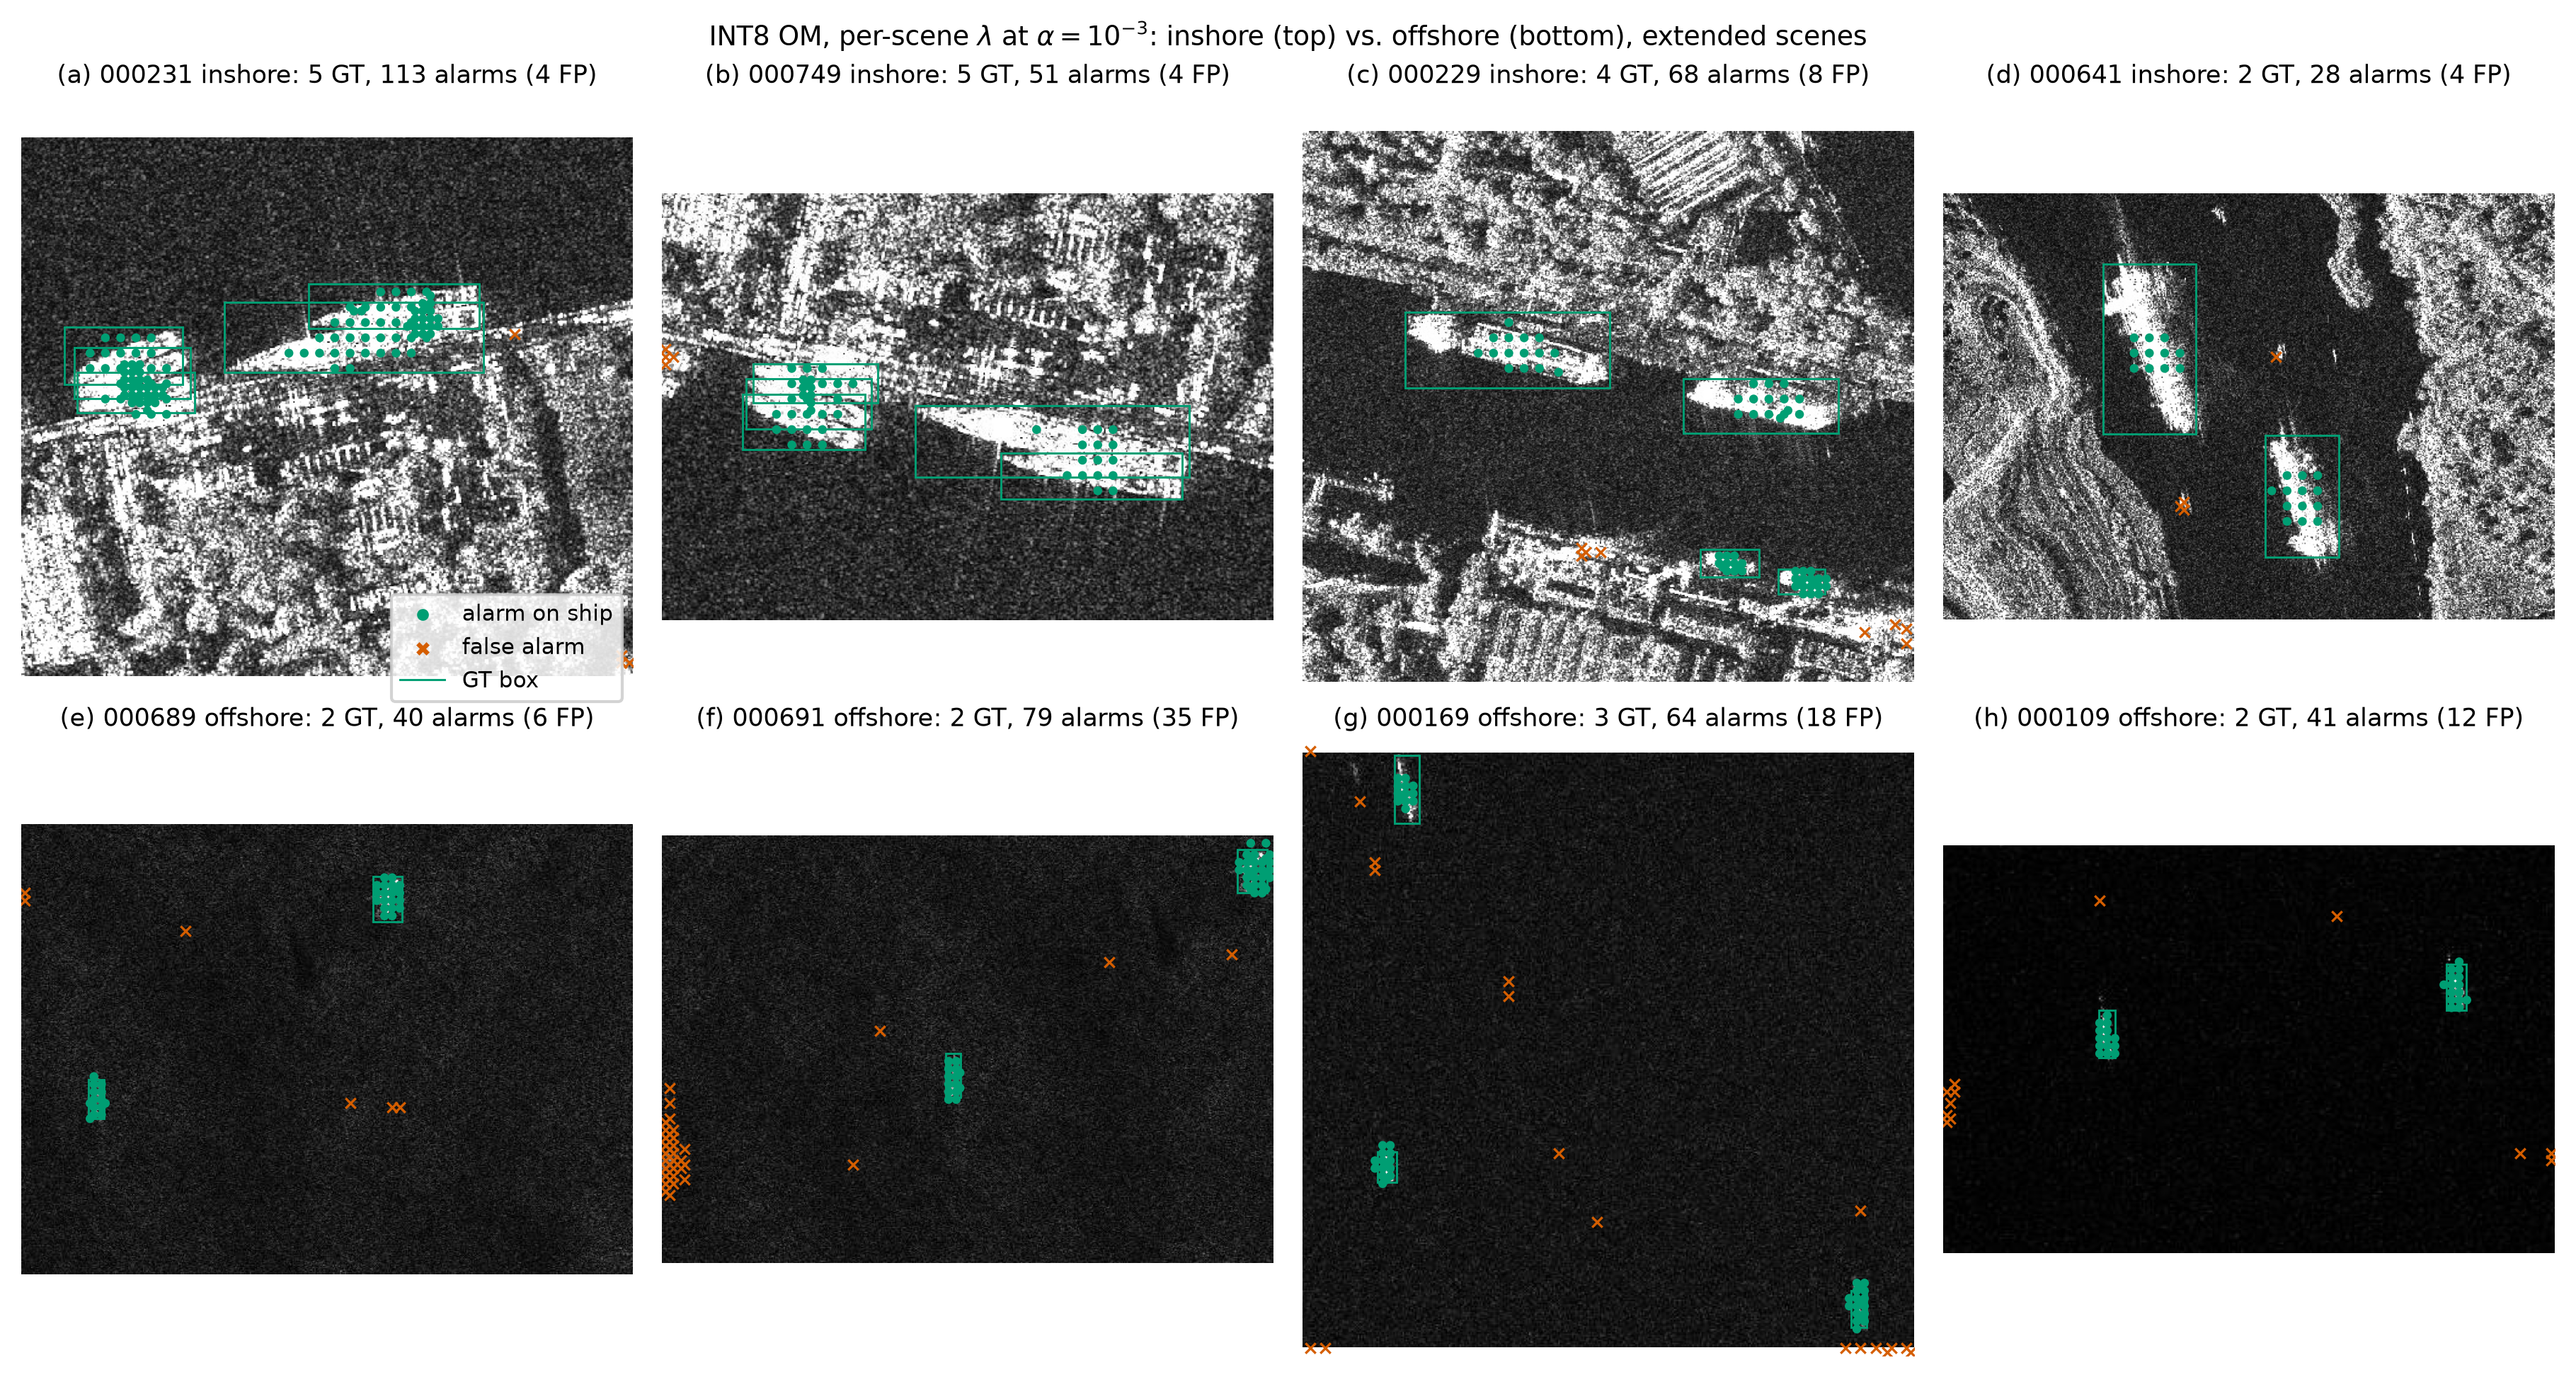
\includegraphics[width=16cm,height=\textheight,keepaspectratio,alt={Fig.20 近岸/远洋扩展场景检测可视化（INT8 OM，逐场景 λ，α=10\^{}-3，与 Fig.18 场景不重叠）：上排近岸（000231 陆地占比 0.267、5 艘；000749、0.261、5 艘；000229、0.255、4 艘；000641、0.226、2 艘），下排远洋（000689 / 000691 / 000169 / 000109，陆地占比 ≈0.001）。框=GT，点=命中，红×=虚警。}]{sample_inshore_det2.png}
\caption*{Fig.20 近岸/远洋扩展场景检测可视化（INT8 OM，逐场景
λ，α=10\^{}-3，与 Fig.18 场景不重叠）：上排近岸（000231 陆地占比
0.267、5 艘；000749、0.261、5 艘；000229、0.255、4 艘；000641、0.226、2
艘），下排远洋（000689 / 000691 / 000169 / 000109，陆地占比
≈0.001）。框=GT，点=命中，红×=虚警。}
\end{figure}

\begin{figure}
\centering
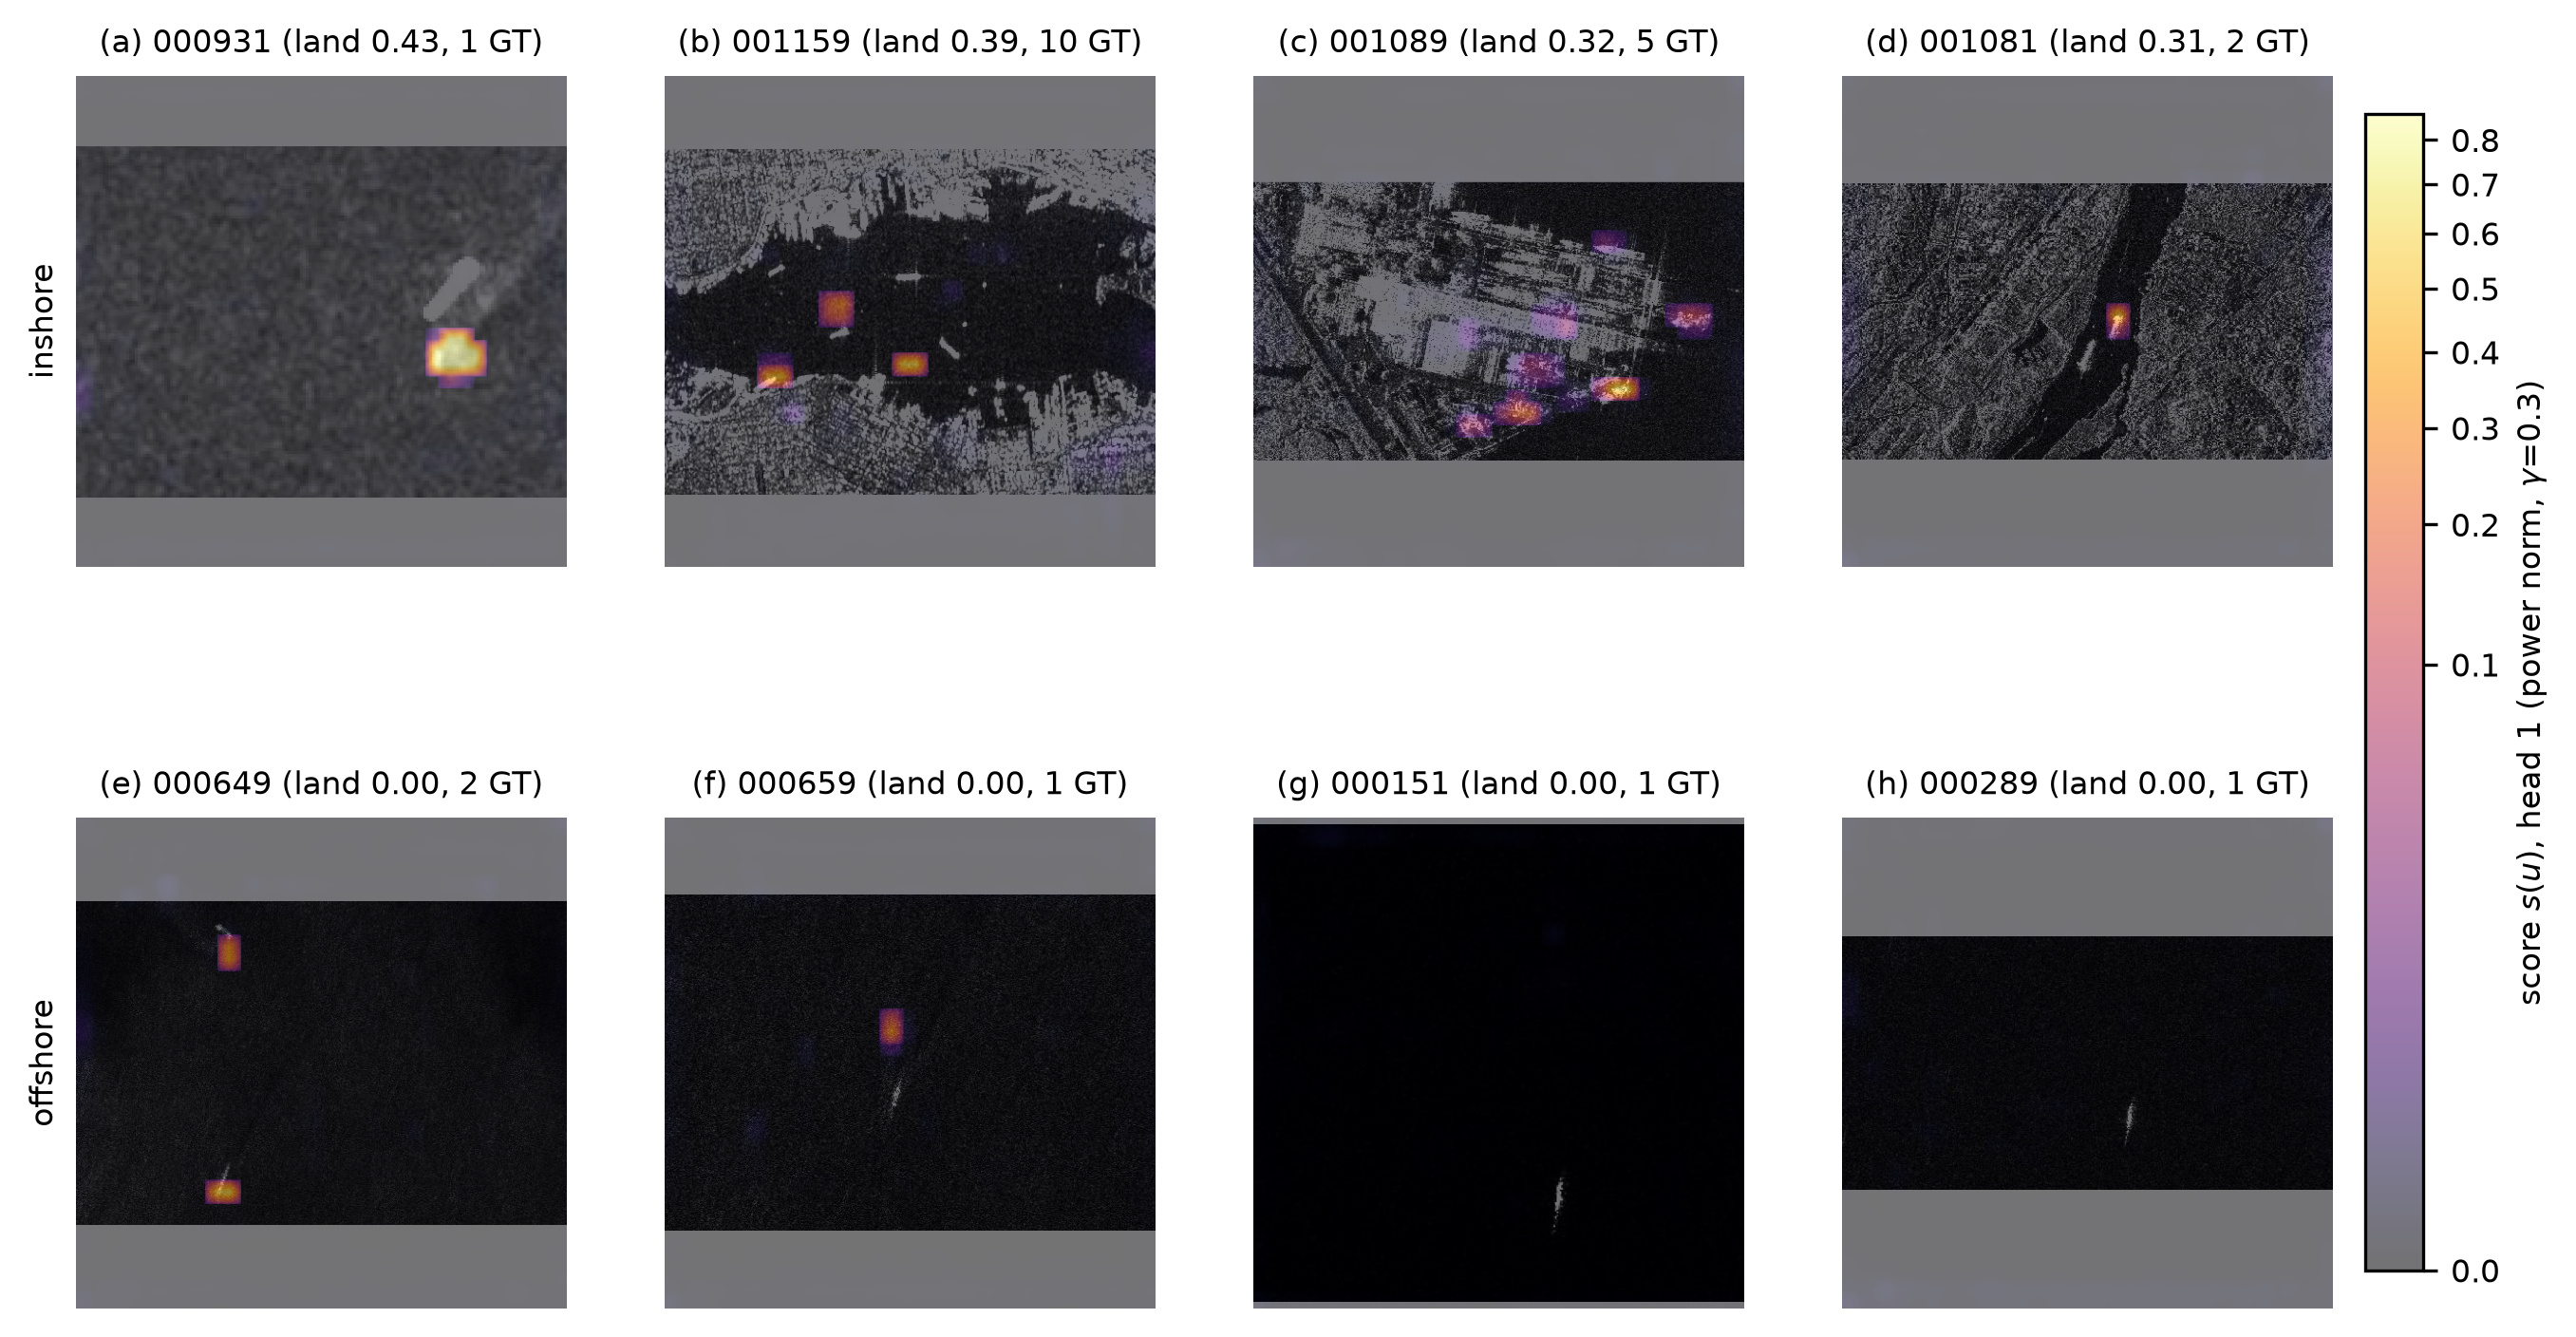
\includegraphics[width=16cm,height=\textheight,keepaspectratio,alt={Fig.21 近岸/远洋场景检测头分数场热图（head 1，power-law 色标，叠加 GT 框）：上排近岸（000931 陆地占比 0.427；001159、0.388、10 艘；001089、0.316、5 艘；001081、0.314、2 艘），下排远洋（000649 / 000659 / 000151 / 000289，陆地占比 ≈0.001）。近岸场景陆地大片高分背景下告警仍集中于舰船位置，直观展示逐场景 λ 的杂波自适应机理。}]{sample_inshore_heat.png}
\caption*{Fig.21 近岸/远洋场景检测头分数场热图（head 1，power-law
色标，叠加 GT 框）：上排近岸（000931 陆地占比 0.427；001159、0.388、10
艘；001089、0.316、5 艘；001081、0.314、2 艘），下排远洋（000649 /
000659 / 000151 / 000289，陆地占比
≈0.001）。近岸场景陆地大片高分背景下告警仍集中于舰船位置，直观展示逐场景
λ 的杂波自适应机理。}
\end{figure}

\begin{figure}
\centering
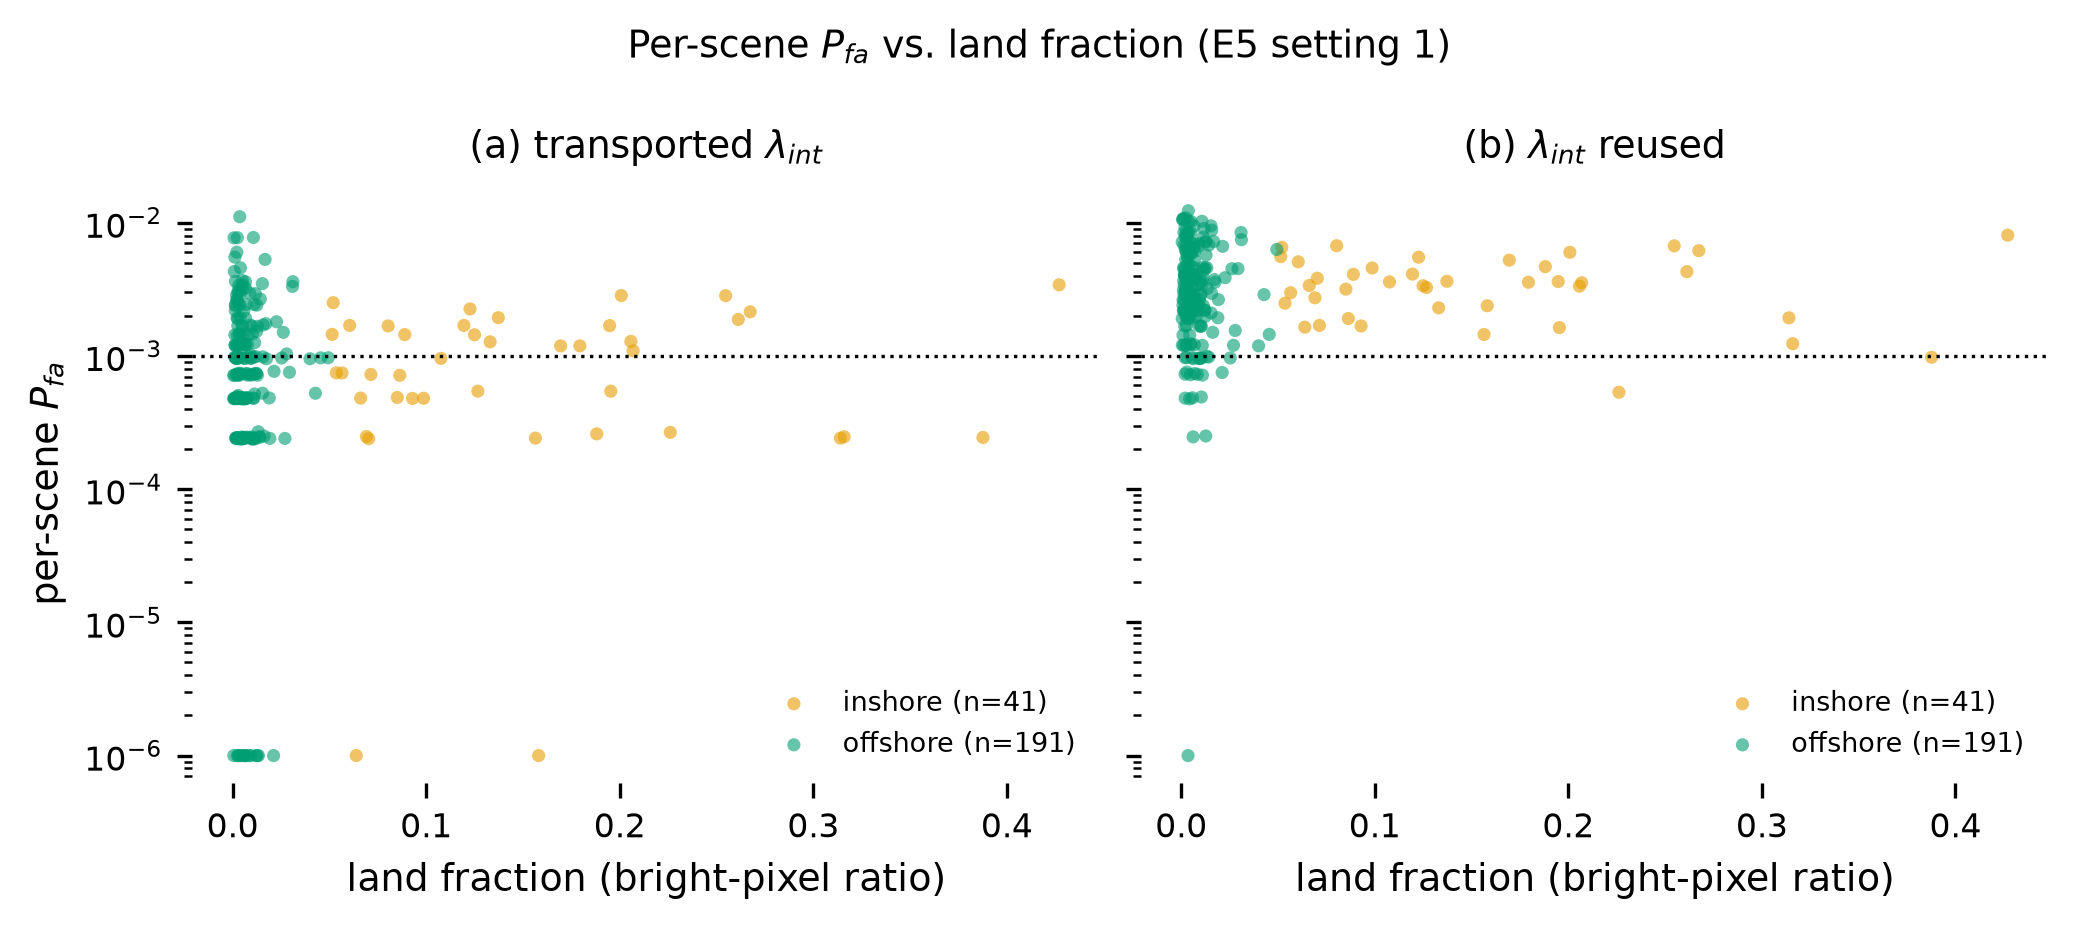
\includegraphics[width=11cm,height=\textheight,keepaspectratio,alt={Fig.22 逐场景 P\_fa 与陆地占比散点（E5 设置1，232 场景，log-y，transport / no\_convert 双面板）：corr(land, log10 P\_fa) 分别为 +0.044 / +0.023，守约性与陆地占比基本不相关。}]{sample_inshore_scatter.png}
\caption*{Fig.22 逐场景 P\_fa 与陆地占比散点（E5 设置1，232
场景，log-y，transport / no\_convert 双面板）：corr(land, log10 P\_fa)
分别为 +0.044 / +0.023，守约性与陆地占比基本不相关。}
\end{figure}

Fig.23 以分组箱线形式对上述散点做统计汇总：近岸（41 场景）与远洋（191
场景）逐场景 \(P_{fa}\)
分布并排对照，三列分别对应搬运、不换算、逐场景重标定（oracle
上界）。关键观察：\textbf{(i) 搬运模式下两组中位数持平}------近岸
\(9.58{\times}10^{-4}\) / 远洋 \(9.52{\times}10^{-4}\)，均紧贴名义
\(\alpha=10^{-3}\)，说明 \(\lambda_{int}\)
换算后的守约性\textbf{不因陆地杂波而系统性偏移}；超过 \(2\alpha\)
的违约场景占比两组亦接近（14.6\% vs 19.4\%）；\textbf{(ii)
不换算对照两组同步恶化}------中位数升至 \(3.55{\times}10^{-3}\) /
\(3.10{\times}10^{-3}\)（超 \(2\alpha\) 违约 75.6\% /
71.2\%），且恶化幅度近岸与远洋相当，印证违约源于量化漂移而非陆地杂波本身；\textbf{(iii)
逐场景重标定上界}两组中位数同样回归 \(\alpha\)
附近（\(9.54{\times}10^{-4}\) /
\(9.73{\times}10^{-4}\)）------搬运解的分组中位数与 oracle
不可区分，是''免数据搬运逼近逐场景重标定''的分组级证据。

\begin{figure}
\centering
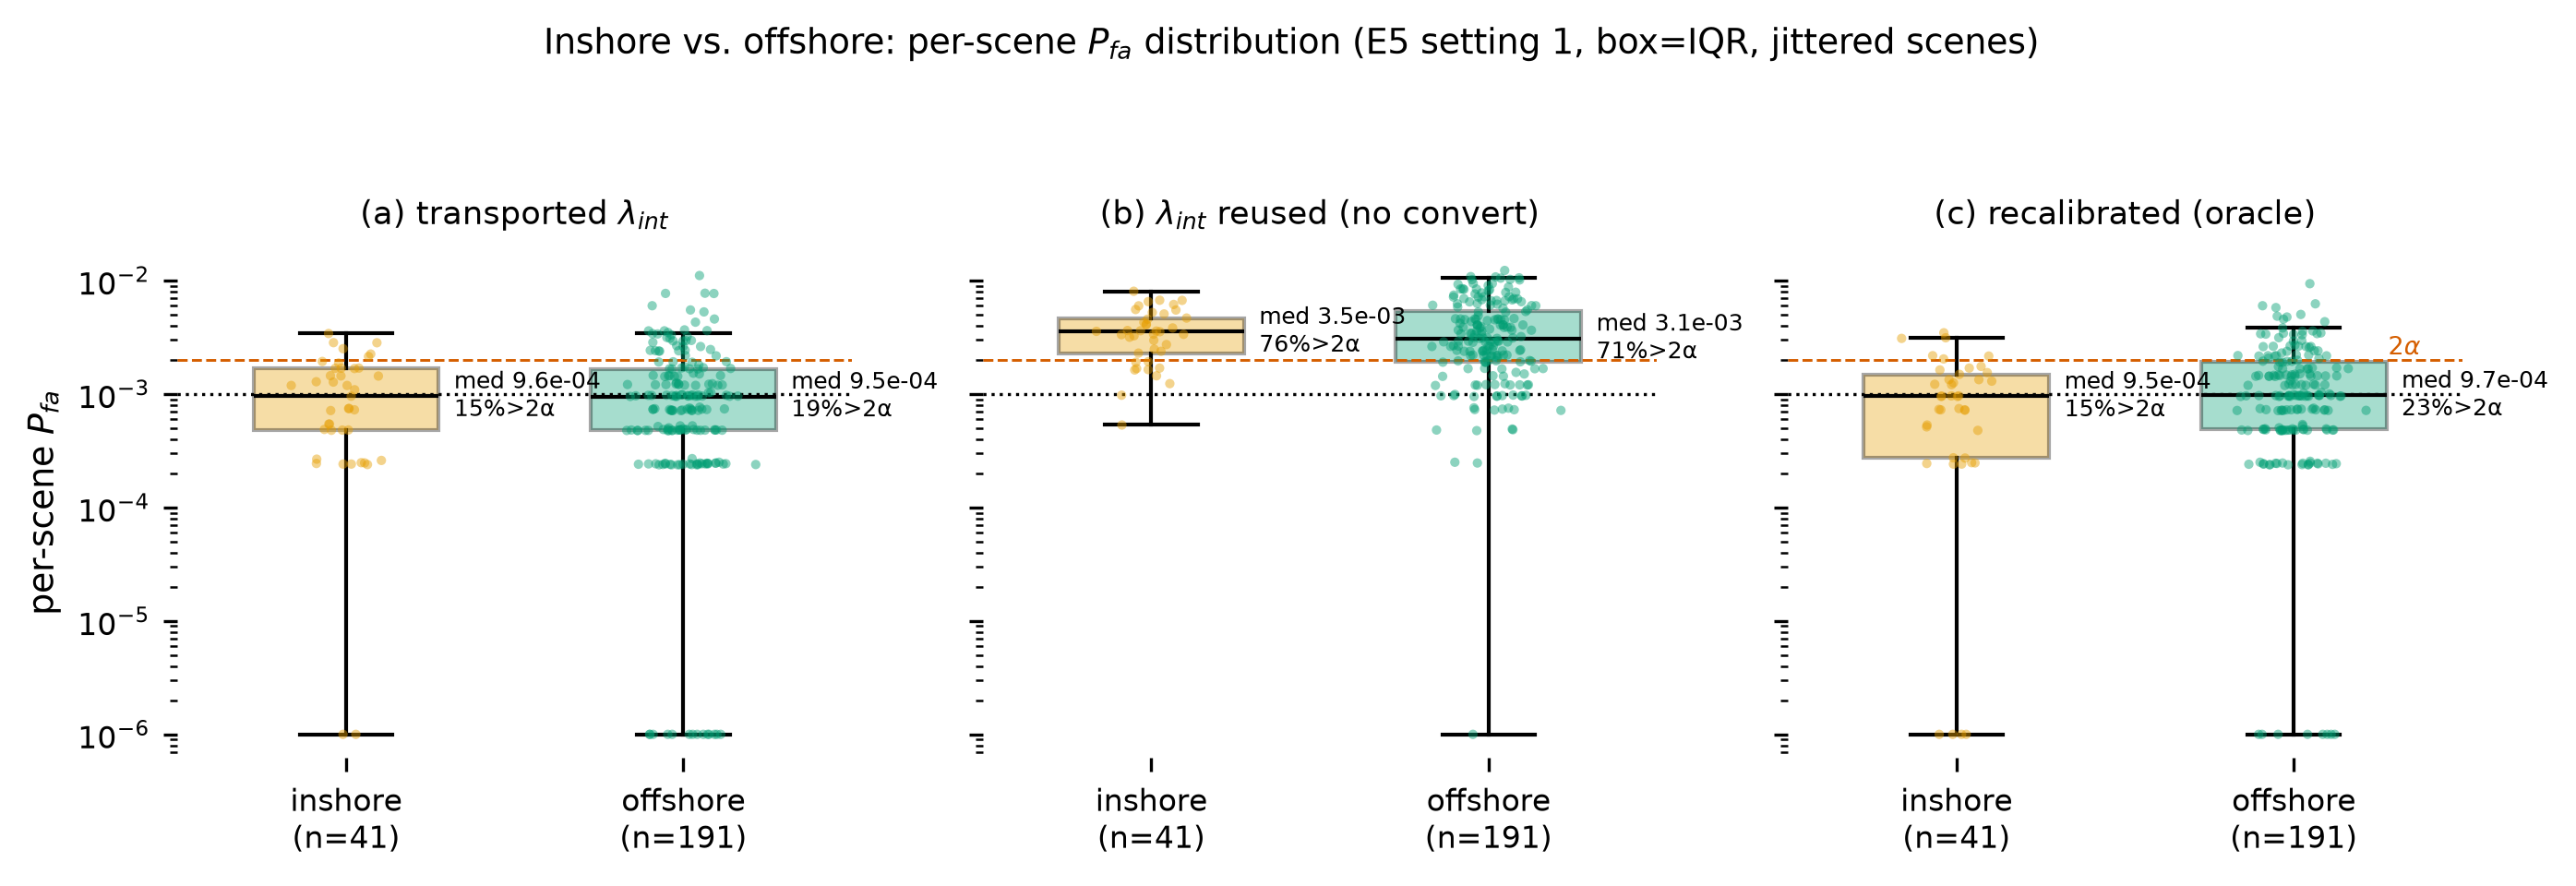
\includegraphics[width=16cm,height=\textheight,keepaspectratio,alt={Fig.23 近岸 vs 远洋逐场景 P\_fa 箱线对比（E5 设置1，近岸 41 / 远洋 191 场景，α=10\^{}-3，log-y，抖动散点叠加）：(a) 搬运 λ\_int；(b) λ\_int 直接复用（不换算）；(c) 逐场景重标定（oracle）。箱体=四分位距，散点=单场景值。搬运两组中位数 9.58e-4 / 9.52e-4 持平且贴 α；不换算两组同步恶化至 3.55e-3 / 3.10e-3（\textgreater2α 违约 75.6\% / 71.2\%）。}]{sample_inshore_box.png}
\caption*{Fig.23 近岸 vs 远洋逐场景 P\_fa 箱线对比（E5 设置1，近岸 41 /
远洋 191 场景，α=10\^{}-3，log-y，抖动散点叠加）：(a) 搬运 λ\_int；(b)
λ\_int 直接复用（不换算）；(c)
逐场景重标定（oracle）。箱体=四分位距，散点=单场景值。搬运两组中位数
9.58e-4 / 9.52e-4 持平且贴 α；不换算两组同步恶化至 3.55e-3 /
3.10e-3（\textgreater2α 违约 75.6\% / 71.2\%）。}
\end{figure}

\begin{center}\rule{0.5\linewidth}{0.5pt}\end{center}

\subsection{{[}E6{]} 热稳态契约保持（只有这块板能做 / Table
7）}\label{e6-ux70edux7a33ux6001ux5951ux7ea6ux4fddux6301ux53eaux6709ux8fd9ux5757ux677fux80fdux505a-table-7}

\textbf{目的}：连续运行至热稳态，区分''一次性测量''与''持续承诺''：温度只能经硬件路径影响推理，A1（整数确定性）预言判决统计量不漂移、时延可能漂移。
\textbf{协议（如实说明）}：板端重放固定杂波帧序列------单图经
\texttt{\_board\_frame\_fn}
预处理一次后复用为恒定输入（\texttt{run\_e6.py}，source=``board''），每窗
200 帧、共 8 窗（40 min），判决阈值 λ 窗外算一次后固定。输入恒定 ⇒ 各窗
\(P_{fa}\) 恒定在 A1 下是\textbf{必然结果}，故本节 \(P_{fa}\) 列仅作
sanity
检查；\textbf{真正的检验量在时延列}（P99、\(T_{model}\)），它承载热稳态漂移的全部信息。

\textbf{Table 7　E6 热稳态逐窗（INT8 复跑，板级 40 min）}

{\def\LTcaptype{none} % do not increment counter
\begin{longtable}[]{@{}lllll@{}}
\toprule\noalign{}
时间窗 & \(P_{fa}\) & P99 (ms) & \(T_{model}\) (ms) & 帧 \\
\midrule\noalign{}
\endhead
\bottomrule\noalign{}
\endlastfoot
0--5 min & \(1.1905{\times}10^{-3}\) & 34.390 & 33.578 & 200 \\
5--10 & \(1.1905{\times}10^{-3}\) & 34.423 & 33.604 & 200 \\
10--15 & \(1.1905{\times}10^{-3}\) & 34.626 & 33.594 & 200 \\
15--20 & \(1.1905{\times}10^{-3}\) & 34.403 & 33.613 & 200 \\
20--25 & \(1.1905{\times}10^{-3}\) & 34.612 & 33.600 & 200 \\
25--30 & \(1.1905{\times}10^{-3}\) & 34.413 & 33.618 & 200 \\
30--35 & \(1.1905{\times}10^{-3}\) & 34.459 & 33.623 & 200 \\
35--40 & \(1.1905{\times}10^{-3}\) & 34.423 & 33.587 & 200 \\
\end{longtable}
}

\textbf{判定}：

{\def\LTcaptype{none} % do not increment counter
\begin{longtable}[]{@{}
  >{\raggedright\arraybackslash}p{(\linewidth - 6\tabcolsep) * \real{0.2500}}
  >{\raggedright\arraybackslash}p{(\linewidth - 6\tabcolsep) * \real{0.2500}}
  >{\raggedright\arraybackslash}p{(\linewidth - 6\tabcolsep) * \real{0.2500}}
  >{\raggedright\arraybackslash}p{(\linewidth - 6\tabcolsep) * \real{0.2500}}@{}}
\toprule\noalign{}
\begin{minipage}[b]{\linewidth}\raggedright
量
\end{minipage} & \begin{minipage}[b]{\linewidth}\raggedright
值
\end{minipage} & \begin{minipage}[b]{\linewidth}\raggedright
阈值
\end{minipage} & \begin{minipage}[b]{\linewidth}\raggedright
通过
\end{minipage} \\
\midrule\noalign{}
\endhead
\bottomrule\noalign{}
\endlastfoot
\(P_{fa}\) 漂移 \(|\log_{10}|\) & \textbf{0.0}（8
窗恒定；重放下的必然结果，仅 sanity） & \(<0.15\) & ✓（弱） \\
P99 跨窗极差 \((max-min)/\bar{T}_{model}\) &
\textbf{0.69\%}（34.390--34.626 ms） & \(<0.15\) & ✓（核心证据） \\
逐窗 headroom \((P99-T_{model})/T_{model}\) & mean \textbf{2.58\%}（max
3.07\%） & \(<0.15\) & ✓ \\
\(T_{model}\) 波动（CV） & \textbf{0.043\%}（33.602 ± 0.015 ms） &
\(<0.15\) & ✓ \\
\textbf{verdict} & \textbf{PASS} & & \\
\end{longtable}
}

\textbf{双运行归属}：Table 7 为 INT8
复跑（\texttt{code/results/e6/}）；第二运行为 asc-sar 仓库的 FP16
板级运行（\texttt{asc-sar/code/results/e6/}，同协议 40 min、8
窗、恒定帧重放），附带温度/功率采样：

{\def\LTcaptype{none} % do not increment counter
\begin{longtable}[]{@{}
  >{\raggedright\arraybackslash}p{(\linewidth - 4\tabcolsep) * \real{0.3333}}
  >{\raggedright\arraybackslash}p{(\linewidth - 4\tabcolsep) * \real{0.3333}}
  >{\raggedright\arraybackslash}p{(\linewidth - 4\tabcolsep) * \real{0.3333}}@{}}
\toprule\noalign{}
\begin{minipage}[b]{\linewidth}\raggedright
量
\end{minipage} & \begin{minipage}[b]{\linewidth}\raggedright
INT8 复跑（Table 7）
\end{minipage} & \begin{minipage}[b]{\linewidth}\raggedright
FP16（asc-sar）
\end{minipage} \\
\midrule\noalign{}
\endhead
\bottomrule\noalign{}
\endlastfoot
\(T_{model}\) & 33.602 ± 0.015 ms（CV 0.043\%） & 27.694 ± 0.082 ms（CV
0.295\%） \\
P99 区间 & 34.390--34.626 ms & 28.160--28.664 ms \\
逐窗 headroom mean（max） & 2.58\%（3.07\%） & 2.17\%（2.71\%） \\
P99 跨窗极差 & 0.69\% & 1.76\% \\
温度 / 功率 & 未采集 & 51.72--53.49 °C / 8.84--8.90 W \\
\end{longtable}
}

\textbf{解读}：\(P_{fa}\) 8 窗恒为
\(1.19{\times}10^{-3}\)------在恒定输入 + A1
下这是必然结果（见协议说明），不构成独立证据，仅确认板端整数判决通路与仿真一致。\textbf{有效证据在时延列}：两配置
40 min 连续负载下 P99 跨窗极差仅 0.69\%（INT8）/
1.76\%（FP16）、\(T_{model}\) CV 0.043\%/0.295\%，均无热漂移趋势；FP16
运行温度 51.7→53.5 °C 缓升期间时延不涨，结合 §4.1.1 遥测说明（CANN
7.0.RC1 对 310B 不提供频率读数，频率列
NaN），以时延稳定性佐证无降频。两个口径勿混：headroom
是逐窗尾延迟相对该窗 \(T_{model}\) 的管线 jitter
裕量，跨窗极差才是热漂移证据。FP16 运行的绝对 \(T_{model}\) 属 asc-sar
变体测量配置，与 E8 benchmark 的 45.5 ms（FP16）不互比；E6
的跨运行结论是''两配置各自 40 min
无漂移趋势''，而非绝对时延对比。本节''只有这块板能做''的价值在于持续 40
min 的板级测量本身，而非 \(P_{fa}\) 恒定性。

\begin{center}\rule{0.5\linewidth}{0.5pt}\end{center}

\subsection{{[}E7{]} 板级系统与''误警→负载''耦合（C3 / Fig.5 / Table
8）}\label{e7-ux677fux7ea7ux7cfbux7edfux4e0eux8befux8b66ux8d1fux8f7dux8026ux5408c3-fig.5-table-8}

\textbf{目的}：在真实部署回路中验证判决层的 host-free
性质（C2），并量化粗糙海况下整数判决对下游候选负载的抑制（C3）；同时给出能效证据。
\textbf{协议}：部署矩阵
\{FP16,INT8\}×\{\textbf{全局模式}（\(\lambda_{\mathrm{glob}}\)，式
3.2a，跨场景混合池标定）, \textbf{QCert 逐场景模式}（\(\lambda(x)\)，式
3.2，逐场景分位标定）\}。海况分桶采用透明可复现的分桶器
\texttt{SeaStateBucketer}（kmeans k=3，特征 = 杂波 cv / Weibull 形状 c /
对比度），232 帧分桶 \{rough:35, medium:174, calm:23\}；负载抑制比取
rough 子集（\(n_{rough}=35\)，产物
\texttt{code/results/e7/table5a\_e7\_v2.csv}）。功率 9.31 W。两列对应
§3.1.1 定义的两个运行点，非两种方法。
\textbf{测量口径（如实）}：判决列系 host 上对整数判决参考实现
\texttt{decide\_simple} 的计时（\texttt{time.perf\_counter}，\(10^4\)
次取中位），即板端判决层耗时的 host 仿真上界，非板上实测；\(T_{model}\)
不取自本实验，直接引用 E8 板级
benchmark（\texttt{code/results/e8/latency.json}，acl\_infer --benchmark
iters=200：FP16 45.5 ms / INT8 34.68 ms）；\(T_{e2e}=T_{model}+\)
判决中位。 \textbf{Limitation（如实）}：负载抑制比仅在 rough
子集（\(n_{rough}=35\)）上实测；逐场景模式''条件误警率均衡 ⇒
候选负载与海况解耦''的机制链仅在本批海况下实测，全海况推广本文不作主张。

\textbf{Table 8　E7 部署矩阵（板级 dump）}

{\def\LTcaptype{none} % do not increment counter
\begin{longtable}[]{@{}
  >{\raggedright\arraybackslash}p{(\linewidth - 14\tabcolsep) * \real{0.1250}}
  >{\raggedright\arraybackslash}p{(\linewidth - 14\tabcolsep) * \real{0.1250}}
  >{\raggedright\arraybackslash}p{(\linewidth - 14\tabcolsep) * \real{0.1250}}
  >{\raggedright\arraybackslash}p{(\linewidth - 14\tabcolsep) * \real{0.1250}}
  >{\raggedright\arraybackslash}p{(\linewidth - 14\tabcolsep) * \real{0.1250}}
  >{\raggedright\arraybackslash}p{(\linewidth - 14\tabcolsep) * \real{0.1250}}
  >{\raggedright\arraybackslash}p{(\linewidth - 14\tabcolsep) * \real{0.1250}}
  >{\raggedright\arraybackslash}p{(\linewidth - 14\tabcolsep) * \real{0.1250}}@{}}
\toprule\noalign{}
\begin{minipage}[b]{\linewidth}\raggedright
配置
\end{minipage} & \begin{minipage}[b]{\linewidth}\raggedright
cand P90(粗糙)
\end{minipage} & \begin{minipage}[b]{\linewidth}\raggedright
判决 ms
\end{minipage} & \begin{minipage}[b]{\linewidth}\raggedright
\(T_{e2e}\) ms
\end{minipage} & \begin{minipage}[b]{\linewidth}\raggedright
P99 ms
\end{minipage} & \begin{minipage}[b]{\linewidth}\raggedright
P99/mean
\end{minipage} & \begin{minipage}[b]{\linewidth}\raggedright
\(P_{fa}\)
\end{minipage} & \begin{minipage}[b]{\linewidth}\raggedright
J/艘
\end{minipage} \\
\midrule\noalign{}
\endhead
\bottomrule\noalign{}
\endlastfoot
FP16-全局 & 42.0 & 0.0238 & 45.525 & 45.538 & 1.00028 &
\(1.000{\times}10^{-3}\) & 0.332 \\
FP16-QCert & \textbf{9.0} & 0.0239 & 45.525 & 45.533 & 1.00018 &
\(1.071{\times}10^{-3}\) & 0.333 \\
INT8-全局 & 44.4 & 0.0244 & 34.705 & 34.712 & 1.00020 &
\(0.999{\times}10^{-3}\) & 0.220 \\
\textbf{INT8-QCert（本文）} & \textbf{9.0} & 0.0242 & 34.705 & 34.710 &
1.00014 & \(1.071{\times}10^{-3}\) & 0.239 \\
\end{longtable}
}

\textbf{判定}：

{\def\LTcaptype{none} % do not increment counter
\begin{longtable}[]{@{}lll@{}}
\toprule\noalign{}
项 & FP16 & INT8 \\
\midrule\noalign{}
\endhead
\bottomrule\noalign{}
\endlastfoot
粗糙 cand P90 比值 全局/QCert & \textbf{4.67×} & \textbf{4.93×} \\
\(\mathrm{pass}_{cand}\)（\(\ge2\times\)） & ✓ & ✓ \\
\(\mathrm{pass}_{dec}\)（\(<3\) ms） & ✓（0.024 ms，host 仿真上界） &
✓ \\
J/艘 drop & 0.997 & 0.921 \\
\end{longtable}
}

\textbf{逐帧 \(P_{fa}\) 违约分布（F3 机制级证据，232 帧；违约 = 逐帧
\(P_{fa}>c\alpha\)，产物
\texttt{code/results/e7/e7\_pf\_summary.json}）}：

{\def\LTcaptype{none} % do not increment counter
\begin{longtable}[]{@{}
  >{\raggedright\arraybackslash}p{(\linewidth - 14\tabcolsep) * \real{0.1250}}
  >{\raggedright\arraybackslash}p{(\linewidth - 14\tabcolsep) * \real{0.1250}}
  >{\raggedright\arraybackslash}p{(\linewidth - 14\tabcolsep) * \real{0.1250}}
  >{\raggedright\arraybackslash}p{(\linewidth - 14\tabcolsep) * \real{0.1250}}
  >{\raggedright\arraybackslash}p{(\linewidth - 14\tabcolsep) * \real{0.1250}}
  >{\raggedright\arraybackslash}p{(\linewidth - 14\tabcolsep) * \real{0.1250}}
  >{\raggedright\arraybackslash}p{(\linewidth - 14\tabcolsep) * \real{0.1250}}
  >{\raggedright\arraybackslash}p{(\linewidth - 14\tabcolsep) * \real{0.1250}}@{}}
\toprule\noalign{}
\begin{minipage}[b]{\linewidth}\raggedright
配置
\end{minipage} & \begin{minipage}[b]{\linewidth}\raggedright
子集
\end{minipage} & \begin{minipage}[b]{\linewidth}\raggedright
median
\end{minipage} & \begin{minipage}[b]{\linewidth}\raggedright
p90
\end{minipage} & \begin{minipage}[b]{\linewidth}\raggedright
max
\end{minipage} & \begin{minipage}[b]{\linewidth}\raggedright
\(>2\alpha\)
\end{minipage} & \begin{minipage}[b]{\linewidth}\raggedright
\(>5\alpha\)
\end{minipage} & \begin{minipage}[b]{\linewidth}\raggedright
\(<\alpha/2\)
\end{minipage} \\
\midrule\noalign{}
\endhead
\bottomrule\noalign{}
\endlastfoot
全局 FP16 & 全 232 & 0.83α & 1.90α & 7.26α & 9.9\% & 1.7\% & 29.3\% \\
全局 FP16 & rough 35 & 0.95α & 5.00α & 7.26α & \textbf{17.1\%} &
\textbf{11.4\%} & 22.9\% \\
全局 INT8 & 全 232 & 0.71α & 2.25α & 7.86α & 11.6\% & 1.7\% & 31.0\% \\
全局 INT8 & rough 35 & 0.95α & 5.29α & 7.86α & \textbf{25.7\%} &
\textbf{11.4\%} & 25.7\% \\
QCert ×\{FP16,INT8\} & 全 232 + rough 35 & 1.07α & 1.07α & 1.07α &
\textbf{0} & \textbf{0} & \textbf{0} \\
\end{longtable}
}

\textbf{解读（性能提升）}： - \textbf{负载降低 4.7--4.9×
的机制是条件误警率的场景间均衡，且有两层独立证据}。候选层（Table
8）：逐场景模式按每场景 \(1-\alpha\) 分位标定 \(\lambda(x)\)，候选数
\(\approx\alpha\,n_{\mathrm{cell}}\) 逐场景恒定（实测各档恒为
9），与场景杂波强度无关；全局模式单一 \(\lambda_{\mathrm{glob}}\)
只在混合分布上保 \(\mathbb{E}[P_{fa}]=\alpha\)，粗糙海况候选 P90 因此达
42.0（FP16 4.67×）/ 44.4（INT8 4.93×）。逐帧违约层（上表）：全局模式的
\(\lambda_{\mathrm{glob}}\) 固定 ⇒
逐帧条件误警率随海况漂移------29.3\%/31.0\% 的帧低于
\(\alpha/2\)（平静侧浪费），粗糙帧 17.1\%/25.7\% 超 \(2\alpha\)、11.4\%
超 \(5\alpha\)（粗糙侧违约），最大漂移 7.26α/7.86α；QCert 逐帧恒为
1.07α（min 0.95α），\textbf{232
帧零违约}。两层证据同向：全局模式的期望守约与逐帧违约并存不矛盾------前者是池化期望的守约，后者正是候选负载随海况膨胀的直接原因；QCert
以逐帧条件误警率均衡换取负载与海况解耦。\textbf{两列总 \(P_{fa}\) 同为
\(\approx\alpha\)（\(1.00\) vs \(1.07\times10^{-3}\)）而候选差近 5
倍，正是两运行点的分工证据而非矛盾}：全局模式优化 pooled 期望精度（E9
err 0.0185），逐场景模式以期望精度为代价（err 0.201，单场景
\(n_{\mathrm{cal}}\) 小）换取负载与海况解耦------下游
NMS/复核负担不再随海况恶化而爆炸（限本批海况，见 Limitation）。 -
\textbf{host-free 证据}：判决层耗时 \(0.024\) ms（host
仿真上界，见协议）\(\ll 3\) ms，host 退出推理回路。 -
\textbf{时延几乎无尾}：P99/mean
\(\approx1.0002\)，端到端时延高度确定（整数判决无数据依赖分支）。 -
\textbf{能效}：INT8-QCert 单船能耗 0.239 J/艘，\(T_{model}=34.68\)
ms（INT8）vs 45.5 ms（FP16），\textbf{提速 1.31×}。

\begin{center}\rule{0.5\linewidth}{0.5pt}\end{center}

\subsection{{[}E8{]} 检测兼容性与对照（Table 9 / Fig.24 /
Fig.36）}\label{e8-ux68c0ux6d4bux517cux5bb9ux6027ux4e0eux5bf9ux7167table-9-fig.24-fig.36}

\textbf{目的}：证明 QCert 不牺牲检测性能，且远超经典
CFAR。\(n_{box}=546\)，232 图。

\textbf{Table 9　E8 兼容性对照（板级 dump）}

{\def\LTcaptype{none} % do not increment counter
\begin{longtable}[]{@{}
  >{\raggedright\arraybackslash}p{(\linewidth - 12\tabcolsep) * \real{0.1429}}
  >{\raggedright\arraybackslash}p{(\linewidth - 12\tabcolsep) * \real{0.1429}}
  >{\raggedright\arraybackslash}p{(\linewidth - 12\tabcolsep) * \real{0.1429}}
  >{\raggedright\arraybackslash}p{(\linewidth - 12\tabcolsep) * \real{0.1429}}
  >{\raggedright\arraybackslash}p{(\linewidth - 12\tabcolsep) * \real{0.1429}}
  >{\raggedright\arraybackslash}p{(\linewidth - 12\tabcolsep) * \real{0.1429}}
  >{\raggedright\arraybackslash}p{(\linewidth - 12\tabcolsep) * \real{0.1429}}@{}}
\toprule\noalign{}
\begin{minipage}[b]{\linewidth}\raggedright
方法
\end{minipage} & \begin{minipage}[b]{\linewidth}\raggedright
\(P_d\)@\(10^{-3}\)
\end{minipage} & \begin{minipage}[b]{\linewidth}\raggedright
\(P_d\)@\(10^{-4}\)
\end{minipage} & \begin{minipage}[b]{\linewidth}\raggedright
mAP50
\end{minipage} & \begin{minipage}[b]{\linewidth}\raggedright
实测 \(P_{fa}\)
\end{minipage} & \begin{minipage}[b]{\linewidth}\raggedright
\(R\)
\end{minipage} & \begin{minipage}[b]{\linewidth}\raggedright
时延 ms
\end{minipage} \\
\midrule\noalign{}
\endhead
\bottomrule\noalign{}
\endlastfoot
CA-CFAR（像素域） & 0.1392 & 0.0751 & --- & \(2.950{\times}10^{-4}\) &
--- & --- \\
YOLO11n + 全局阈值 & 0.9945 & 0.9872 & 98.27 & \(1.037{\times}10^{-3}\)
& --- & 45.5 \\
YOLO11n + QCert(FP16) & 0.9908 & --- & 98.27 & \(1.741{\times}10^{-3}\)
& 1.0 & 45.5 \\
YOLO11n + QCert(INT8) & 0.9908 & 0.9853 & 97.98 &
\(1.741{\times}10^{-3}\) & 1.0 & 34.68 \\
\textbf{QCert（完整）} & 0.9908 & 0.9853 & 97.98 &
\(1.741{\times}10^{-3}\) & 1.0 & 34.68 \\
\end{longtable}
}

\begin{quote}
\textbf{标定协议（重要）}：Table 9 每一行在各自配置下\textbf{独立重标定}
λ（FP16 行用 FP16 杂波分布、INT8 行用 INT8 分布，见 \texttt{run\_e8.py}
\texttt{\_lambda\_global}），故 QCert(FP16) 与 QCert(INT8) 的实测
\(P_{fa}\) 同为 \(1.741{\times}10^{-3}\)
是''各自最优标定''的结果，而非同一 λ 跨配置直接复用------后者恰是 E5
设置 2 所检验的搬运问题。QCert 各行均采用\textbf{全局模式}（式
3.2a，\texttt{\_lambda\_global} 为跨场景混合池标定）；逐场景模式（式
3.2）的负载特性见 E7。 \textbf{CA-CFAR 定位}：像素域 CA-CFAR
为\textbf{未调优的 strawman
基线}（guard=2、train=8，其余默认），其网格参数未精确命中
\(\alpha\)（实测 \(2.95{\times}10^{-4}\) 低于名义 \(10^{-3}\)，\(P_d\)
随之下压），仅作数量级对照，不构成公平竞争对手。
\textbf{测量粒度注（\(\alpha\) 可达性，F2 定量交代）}：Table 9 各行的
\(\alpha\) 口径受标定池有效样本量约束。按块内样本强相关折算的独立单元数
\(n_{\mathrm{eff}}\) 逐场景仅 min 45 / median 50（\(n_{\mathrm{meas}}\)
median 4116，产物
\texttt{code/results/e8/e8\_neff\_summary.json}），故单场景可辨识的
\(\alpha\) 下限 \(\sim 1/n_{\mathrm{eff}}\approx0.02\)（与 §3.3.1 的
\(\alpha\ge1/(n_{\cal}+1)\) 下界一致）：\(\alpha=10^{-3}\) 档要求
\(n_{\mathrm{eff}}\ge10^{3}\)，实测\textbf{没有任何场景}满足（比例
0.000）；逐场景 \(P_{fa}\) 的量化步长 \(1/n_{\mathrm{meas}}\) median 为
\(2.43{\times}10^{-4}>\alpha\)。因此 Table 9 的实测 \(P_{fa}\) 与
\(P_d\)@\(10^{-4}\)/\(10^{-3}\)
各档均为\textbf{跨场景合并}估计，\(\alpha\le\)
逐场景量化步长的工作点不是本文可验证的口径。
\end{quote}

\textbf{判定}：

{\def\LTcaptype{none} % do not increment counter
\begin{longtable}[]{@{}llll@{}}
\toprule\noalign{}
项 & 值 & 阈值 & 通过 \\
\midrule\noalign{}
\endhead
\bottomrule\noalign{}
\endlastfoot
\(P_d\) gap vs 最强基线 & \(-0.0037\) & \(\ge-0.015\) & ✓ \\
\(R\) & 1.0 & \(\le1.2\) & ✓ \\
\(\Delta\)mAP50 & \(-0.29\) 点 & \(\le0.5\) 点 & ✓ \\
\(P_{fa}\)@\(10^{-4}\) 可达 & True & --- & ✓ \\
\textbf{pass} & \textbf{True} & & \\
\end{longtable}
}

\textbf{解读（性能提升）}： -
\textbf{兼容性无损}：相对最强复现基线（YOLO11n+全局阈值）\(P_d\) 仅差
0.37 点，远优于 \(-1.5\) 点验收线；mAP 损失 0.29 点；\(R=1.0\)。 -
\textbf{远超 CA-CFAR}：\(P_d\) 0.991 vs 0.139（\textbf{7
倍}）------``你不是 CFAR''的辩护成立：QCert
在承诺误警率的同时，检测力远超像素域 CFAR。 - \textbf{INT8 提速}：34.68
ms vs FP16 45.5 ms，\textbf{1.31×}，且 \(P_d\) 不降。

Fig.24 将 Table 9 的对照数字可视化为三面板柱状图：\textbf{(a)
检测力}------\(P_d@10^{-3}\) / \(P_d@10^{-4}\) 双柱对照，QCert(INT8)
0.9908 / 0.9853 与 YOLO11n+全局阈值 0.9945 / 0.9872 几乎并排（gap 0.37 /
0.19 点），CA-CFAR 仅 0.1392 / 0.0751，7 倍差距一目了然；\textbf{(b)
实测 \(P_{fa}\) vs 契约带}------log 轴柱高叠加 \([\alpha, 2\alpha]\)
阴影带（\(\alpha=10^{-3}\)）：QCert FP16/INT8 同为
\(1.741{\times}10^{-3}\)，落于契约带上沿附近（\(R=1.0\)，在 \(2\alpha\)
容差内）；全局阈值 \(1.037{\times}10^{-3}\)
亦在带内但\textbf{无契约保证}（阈值不可跨配置搬运，见 E5 设置
2）；\textbf{(c) 板级时延}------INT8 34.68 ms 对 FP16 45.5 ms 的 1.31×
加速以箭头标注，直观呈现量化部署收益。

\begin{figure}
\centering
\includegraphics[width=16cm,height=\textheight,keepaspectratio,alt={Fig.24 E8 对照/SOTA 可视化对比（板级 dump，α=10\^{}-3，契约带 {[}α,2α{]}）：(a) P\_d@10\^{}-3 / 10\^{}-4 双柱------CA-CFAR 0.1392 / 0.0751，全局阈值 0.9945 / 0.9872，QCert(INT8) 0.9908 / 0.9853；(b) 实测 P\_fa（log-y）------QCert 1.741e-3 落契约带，全局阈值 1.037e-3 在带内但无搬运保证；(c) 时延------34.68 vs 45.5 ms（1.31× 提速）。}]{sample_sota_bar.png}
\caption*{Fig.24 E8 对照/SOTA 可视化对比（板级 dump，α=10\^{}-3，契约带
{[}α,2α{]}）：(a) P\_d@10\^{}-3 / 10\^{}-4 双柱------CA-CFAR 0.1392 /
0.0751，全局阈值 0.9945 / 0.9872，QCert(INT8) 0.9908 / 0.9853；(b) 实测
P\_fa（log-y）------QCert 1.741e-3 落契约带，全局阈值 1.037e-3
在带内但无搬运保证；(c) 时延------34.68 vs 45.5 ms（1.31× 提速）。}
\end{figure}

Fig.36 将本文与\textbf{公开 SOTA
及相关工作}放入同一坐标系做三面板对比（配合 §2 Table 0
的覆盖矩阵）：\textbf{(a) SSDD mAP50 横向对比}------AC-YOLO
96.7、BESW-YOLO 97.3、LSD-DETR 97.3、LAMFDet 99.5（公开论文口径），本文
FP16 98.27 / INT8+QCert 97.98：INT8+QCert 落在
AC-YOLO/BESW-YOLO/LSD-DETR 之上，且距自身 FP16 仅 0.29 点，远在 ±1 mAP
的量化部署验收门限内（绿色带）------即''契约保证几乎不花精度预算''；LAMFDet
99.5 系同数据集上的专门化架构，其数字不含任何
\(P_{fa}\)/板级契约主张（见 (b) 列）。\textbf{(b) 审计维度覆盖矩阵}（§2
Table 0 的可视化）：SAR 检测 SOTA 只覆盖''报 mAP''一列；PTQ/QAT
工作线覆盖 mAP + 部分定点算术/板级实测，但均无尾分位数 \(P_{fa}\)@α
主张；经典 CFAR/CFARnet 有 \(P_{fa}\)
主张但无学习检测力与板级部署；conformal
系（SeqCRC）无杂波建模亦无板级；唯本文 QCert
在五个审计维度上全覆盖。\textbf{(c) \(P_d@10^{-3}\)
板级对照}------CA-CFAR（strawman）0.139、YOLO11n+全局阈值
0.995、QCert(INT8) 0.991，配 1.31× 提速注记：检测力与契约保证同框成立。

\begin{figure}
\centering
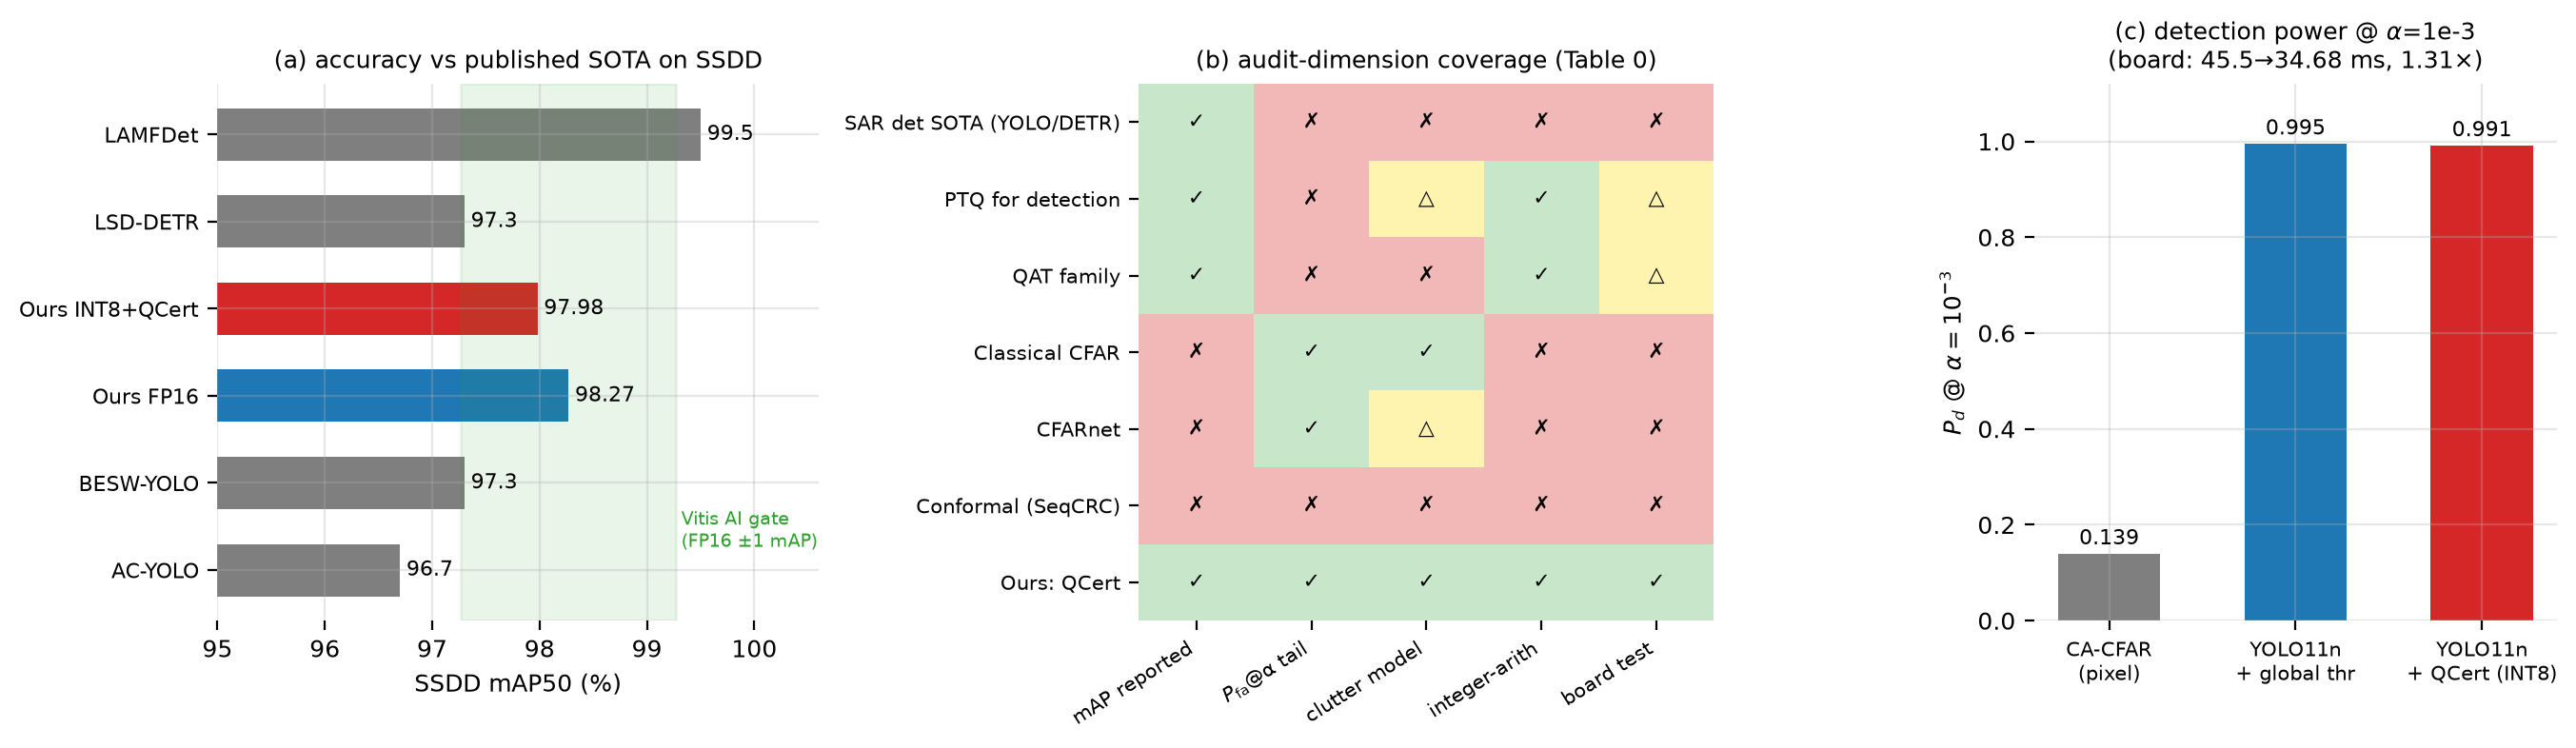
\includegraphics[width=16cm,height=\textheight,keepaspectratio,alt={Fig.36 与 SOTA / 相关工作对比三面板：(a) SSDD mAP50------AC-YOLO 96.7、BESW-YOLO 97.3、LSD-DETR 97.3、LAMFDet 99.5 vs 本文 FP16 98.27 / INT8+QCert 97.98（绿色带 = FP16±1 mAP 量化验收门限，INT8 距 FP16 仅 0.29 点）；(b) Table 0 审计维度覆盖矩阵（✓/✗/△，唯 QCert 五维全覆盖）；(c) P\_d@α=1e-3 板级对照------CA-CFAR 0.139 / 全局阈值 0.995 / QCert(INT8) 0.991，附 1.31× 提速。}]{fig33_sota_compare.png}
\caption*{Fig.36 与 SOTA / 相关工作对比三面板：(a) SSDD
mAP50------AC-YOLO 96.7、BESW-YOLO 97.3、LSD-DETR 97.3、LAMFDet 99.5 vs
本文 FP16 98.27 / INT8+QCert 97.98（绿色带 = FP16±1 mAP
量化验收门限，INT8 距 FP16 仅 0.29 点）；(b) Table 0
审计维度覆盖矩阵（✓/✗/△，唯 QCert 五维全覆盖）；(c) P\_d@α=1e-3
板级对照------CA-CFAR 0.139 / 全局阈值 0.995 / QCert(INT8) 0.991，附
1.31× 提速。}
\end{figure}

\begin{center}\rule{0.5\linewidth}{0.5pt}\end{center}

\subsection{{[}E9{]} 消融与失败分析（Table 10 / Fig.25--29 /
Fig.35）}\label{e9-ux6d88ux878dux4e0eux5931ux8d25ux5206ux6790table-10-fig.2529-fig.35}

\textbf{目的}：支撑方法论选择（块抽样、标定样本量、全局 vs
逐场景、除法消除、桶数）。

\textbf{Table 10a　E9 块抽样 keep 比（真实，232 图，reps=10）}

{\def\LTcaptype{none} % do not increment counter
\begin{longtable}[]{@{}llll@{}}
\toprule\noalign{}
keep & \(P_{fa}\) & err & \(n_{\mathrm{eff}}\) \\
\midrule\noalign{}
\endhead
\bottomrule\noalign{}
\endlastfoot
1.0 & \(1.590{\times}10^{-3}\) & 0.201 & 49.8 \\
0.25 & \(1.769{\times}10^{-3}\) & 0.248 & 24.9 \\
0.125 & \(2.372{\times}10^{-3}\) & 0.375 & 12.0 \\
0.0625 & \(4.717{\times}10^{-3}\) & 0.674 & 6.0 \\
\end{longtable}
}

\begin{quote}
注：err \(=|\log_{10}(P_{fa}/\alpha)|\)（偏离度，与 §4.1.4
契约度量同口径）；\(n_{\mathrm{eff}}\)
为测量块数（块抽样后，场景均值）。keep 下降同时压缩标定池
\(n_{\mathrm{cal}}\) 与 \(n_{\mathrm{eff}}\)：keep=0.0625 档
\(n_{\mathrm{cal}}\approx5\times10^{2}\)，契约下界
\(\alpha\ge1/(n_{\mathrm{cal}}+1)\approx2\times10^{-3}\) 已高于名义
\(\alpha=10^{-3}\)，该档 \(P_{fa}=4.7\times10^{-3}\)
恰被顶到下界量级------err 随 keep 的单调恶化是秩涨落放大与 \(\alpha\)
下界抬升的共同结果（式 3.5 声明
(i)），是本表的理论解读而非异常。keep=1.0 行的 60\% 偏离与 E0 表
FP16/INT8 的绝对水平（\(D\approx0.33\)）同因------标定与测量集构造差异 +
有限标定池，\textbf{与 E0 的 NO-GO 判定无因果关系}：E0 由存在性门
\(R=0.969<1.5\) 判定，与 \(P_{fa}\) 绝对水平无关。
\end{quote}

Fig.25 以折线形式呈现该扫描的两面：(a) \(P_{fa}\) 随 keep
下降的单调抬升；(b) 契约误差 err 与有效测量块数 \(n_{\mathrm{eff}}\)
的关系------err 增长曲线与有限样本秩涨落的理论预期一致。

\begin{figure}
\centering
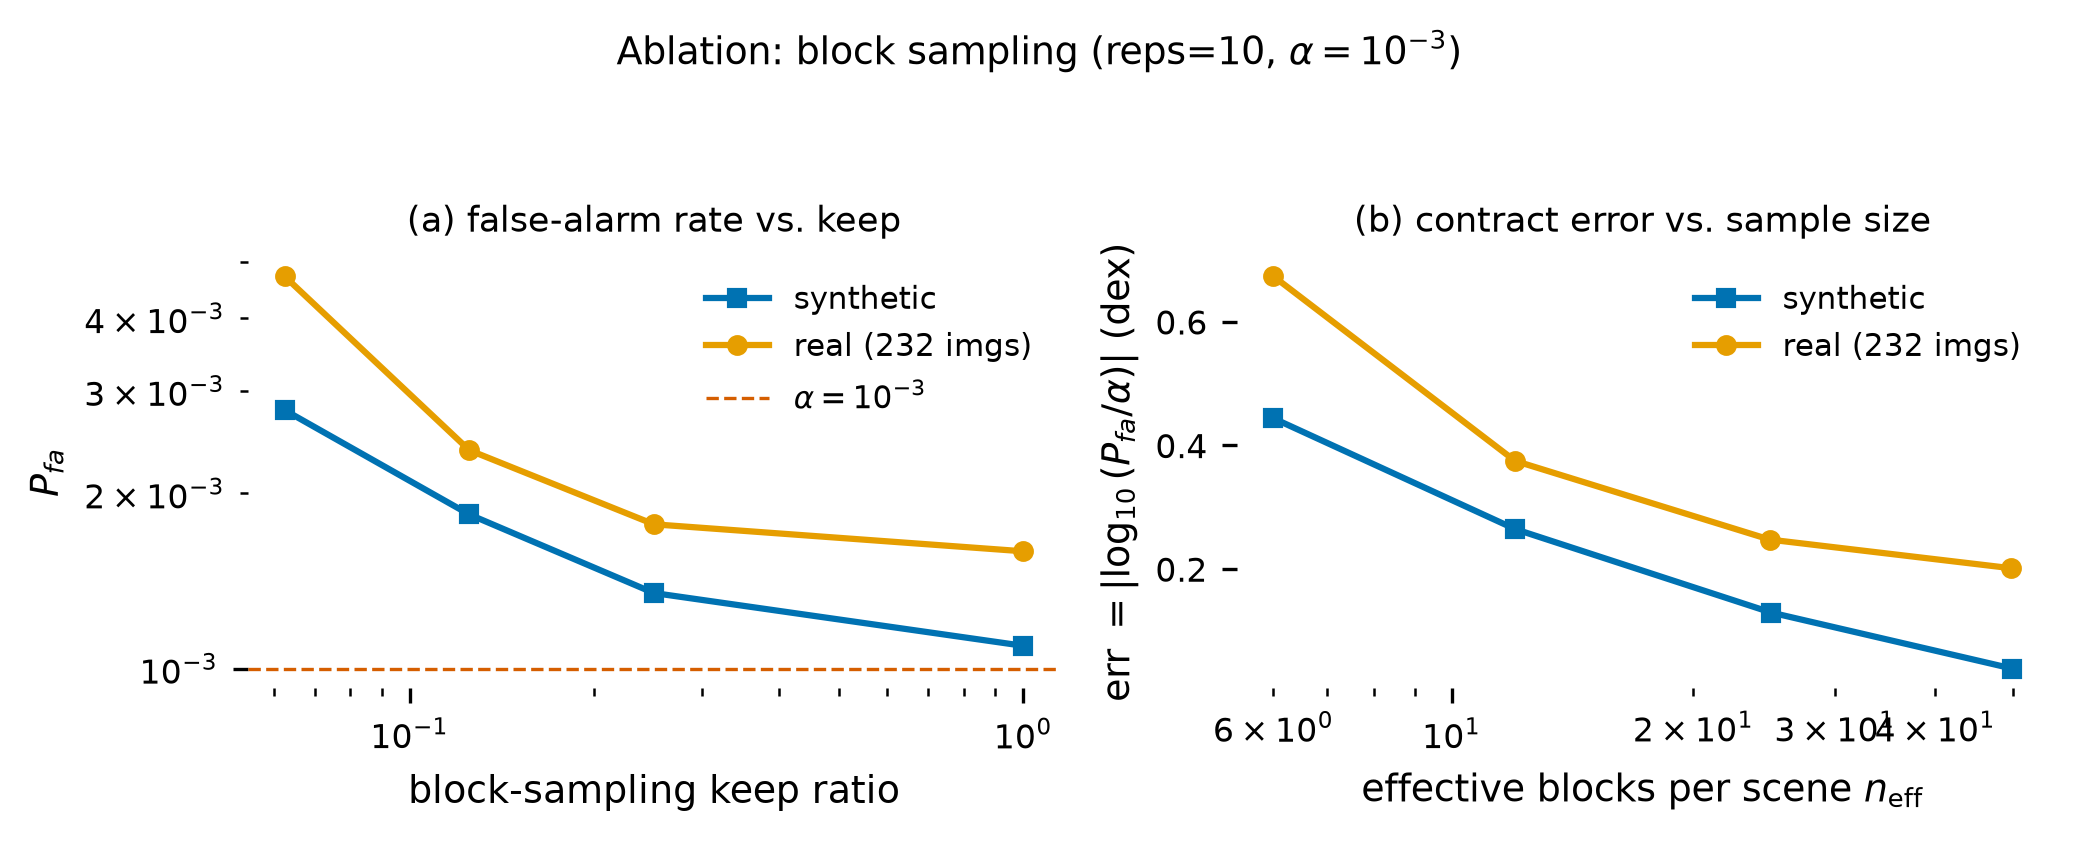
\includegraphics[width=11cm,height=\textheight,keepaspectratio,alt={Fig.25 块抽样 keep 比扫描（真实 232 图，reps=10，α=10\^{}-3）：(a) P\_fa vs keep；(b) 契约误差 err=\textbar log10(P\_fa/α)\textbar{} vs 有效测量块数 n\_eff。}]{sample_ablation_keep.png}
\caption*{Fig.25 块抽样 keep 比扫描（真实 232
图，reps=10，α=10\^{}-3）：(a) P\_fa vs keep；(b) 契约误差
err=\textbar log10(P\_fa/α)\textbar{} vs 有效测量块数 n\_eff。}
\end{figure}

\textbf{Table 10b　E9 标定样本量（真实）}

{\def\LTcaptype{none} % do not increment counter
\begin{longtable}[]{@{}lll@{}}
\toprule\noalign{}
n & 相对误差 mean & std \\
\midrule\noalign{}
\endhead
\bottomrule\noalign{}
\endlastfoot
16 & 0.0886 & 0.0810 \\
64 & 0.0802 & 0.0573 \\
128 & \textbf{0.0757} & 0.0618 \\
200 & 0.1510 & 0.1291 \\
\end{longtable}
}

\begin{quote}
注：n=200
误差反升系块抽样边界效应------标定场景数接近全量时，抽样块与测量块的重叠方差增大（底稿记录）；本文据此取
n=128 为标定规模。
\end{quote}

Fig.26 给出该扫描的误差-带（mean±std，reps=10）：n=128
处于误差平台的最低段，n=200 的反升清晰可见，n=16--128
段样本量收益递减------为''标定集 128 图''的工程选择提供曲线依据。

\begin{figure}
\centering
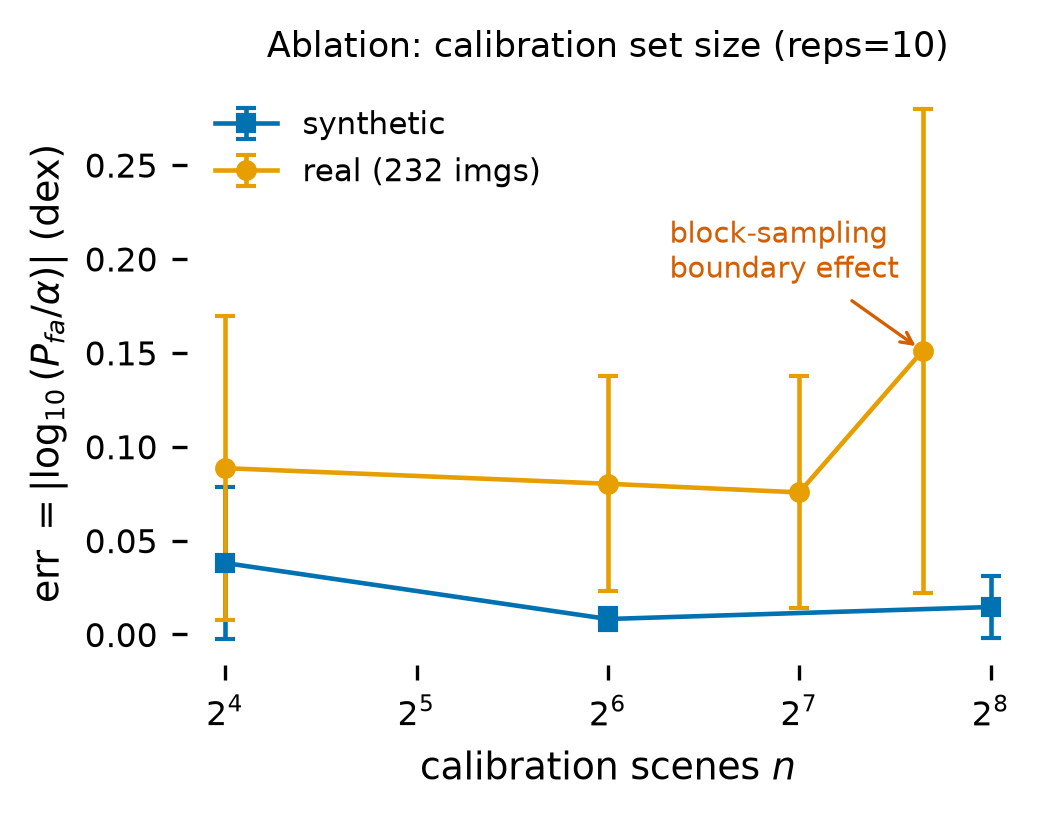
\includegraphics[width=11cm,height=\textheight,keepaspectratio,alt={Fig.26 标定样本量扫描（真实，reps=10）：契约误差 err=\textbar log10(P\_fa/α)\textbar（mean±std）vs 标定场景数 n∈\{16, 64, 128, 200\}；n=128 为平台最低段，n=200 因块抽样边界效应反升。}]{sample_ablation_ncal.png}
\caption*{Fig.26 标定样本量扫描（真实，reps=10）：契约误差
err=\textbar log10(P\_fa/α)\textbar（mean±std）vs 标定场景数 n∈\{16, 64,
128, 200\}；n=128 为平台最低段，n=200 因块抽样边界效应反升。}
\end{figure}

\textbf{Table 10c　E9 逐场景 vs 全局标定（真实）}

{\def\LTcaptype{none} % do not increment counter
\begin{longtable}[]{@{}
  >{\raggedright\arraybackslash}p{(\linewidth - 8\tabcolsep) * \real{0.2000}}
  >{\raggedright\arraybackslash}p{(\linewidth - 8\tabcolsep) * \real{0.2000}}
  >{\raggedright\arraybackslash}p{(\linewidth - 8\tabcolsep) * \real{0.2000}}
  >{\raggedright\arraybackslash}p{(\linewidth - 8\tabcolsep) * \real{0.2000}}
  >{\raggedright\arraybackslash}p{(\linewidth - 8\tabcolsep) * \real{0.2000}}@{}}
\toprule\noalign{}
\begin{minipage}[b]{\linewidth}\raggedright
方案
\end{minipage} & \begin{minipage}[b]{\linewidth}\raggedright
\(P_{fa}\)
\end{minipage} & \begin{minipage}[b]{\linewidth}\raggedright
\(P_d\)（单元级汇总）
\end{minipage} & \begin{minipage}[b]{\linewidth}\raggedright
标定误差 err
\end{minipage} & \begin{minipage}[b]{\linewidth}\raggedright
期望精度口径采用
\end{minipage} \\
\midrule\noalign{}
\endhead
\bottomrule\noalign{}
\endlastfoot
逐场景 & \(1.590{\times}10^{-3}\) & 0.1863 & 0.2014 & --- \\
\textbf{全局} & \(\mathbf{1.043{\times}10^{-3}}\) & 0.1828 &
\textbf{0.0185} & ✓ \\
\end{longtable}
}

\begin{quote}
注：本表 \(P_d\) 为杂波/目标单元级汇总口径，与 Table 9 的框级
\(P_d\)（0.99）不可直接比较。 注：全局行 err=0.0185 dex（相对偏差仅
4.3\%）\textbf{低于 §3.1.1 的有限样本噪声底}，系 λ
与测量在同一杂波池上标定（in-sample）所致的乐观偏差，应视为标定分辨率（整数分位数
B=4096）下的\textbf{下界}而非泛化精度；逐场景行 err 含跨场景泛化误差故大
10×。
\end{quote}

→ \textbf{期望精度口径下全局模式占优}（err 低 10×，\(P_d\) 仅差
0.0035），本文全局模式（式
3.2a）采用之。但这不是对逐场景模式的否定：逐场景模式以 err 0.201
为代价换取\textbf{条件误警率均衡与候选负载恒定}------E7 的 4.7--4.9×
负载抑制正来源于此。二者是 §3.1.1
定义的两个合法运行点，按部署瓶颈（期望精度 vs
负载/尾时延）二选一，不可读作''同一配置同时取得两个数字''。

\textbf{Table 10d　E9 合成项（items 1/2/8）}

{\def\LTcaptype{none} % do not increment counter
\begin{longtable}[]{@{}
  >{\raggedright\arraybackslash}p{(\linewidth - 2\tabcolsep) * \real{0.5000}}
  >{\raggedright\arraybackslash}p{(\linewidth - 2\tabcolsep) * \real{0.5000}}@{}}
\toprule\noalign{}
\begin{minipage}[b]{\linewidth}\raggedright
项
\end{minipage} & \begin{minipage}[b]{\linewidth}\raggedright
关键结果
\end{minipage} \\
\midrule\noalign{}
\endhead
\bottomrule\noalign{}
\endlastfoot
除法消除 divfree & \(P_{fa}\) 漂移 0.0140 dex，判决不一致率
\(1.69{\times}10^{-3}\) → \textbf{有效} \\
零量化 zquant & 漂移 0.0124 dex → 有效 \\
桶数 \(B\)=4096 & \(\alpha\) 误差 0.084 dex，\(\lambda\) 误差
\(|\Delta z|=0.0059\) → \textbf{达标} \\
标度指数 round / floor & 2.055 / 1.268（round 更符合
\(\varepsilon^2\)） \\
\end{longtable}
}

\begin{quote}
注：items 1/2 依赖 \(\mu/\sigma\) 结构留合成版；items 6/7 展开见 Table
10e/10f。
\end{quote}

\textbf{Table 10e　E9 分数归一化 h0 消融（item 6，合成，SSDD 232）}

{\def\LTcaptype{none} % do not increment counter
\begin{longtable}[]{@{}lll@{}}
\toprule\noalign{}
设置 & \(R\)（INT8/FP32） & \(P_d@10^{-3}\)（INT8） \\
\midrule\noalign{}
\endhead
\bottomrule\noalign{}
\endlastfoot
\(z=(s-\mu)/\sigma\)（含 \(h_0\)） & 1.033 & 0.582 \\
原始分数 \(s\)（去 \(h_0\)） & 0.917 & 0.178 \\
\end{longtable}
}

\begin{quote}
注：去掉归一化后 \(R\) 漂离 1 达 8.3\%，INT8 与 FP32
的判决统计量跨配置不再可比------阈值搬运（E5）的前提失效；\(P_d\) 崩塌
3.3×（−69\%）。归一化是式 (3.2a) 前提 \(h_0\) 成立的消融证据。
\end{quote}

\textbf{Table 10f　E9 校准集分层消融（item 7，合成，压测集）}

{\def\LTcaptype{none} % do not increment counter
\begin{longtable}[]{@{}
  >{\raggedright\arraybackslash}p{(\linewidth - 8\tabcolsep) * \real{0.2000}}
  >{\raggedright\arraybackslash}p{(\linewidth - 8\tabcolsep) * \real{0.2000}}
  >{\raggedright\arraybackslash}p{(\linewidth - 8\tabcolsep) * \real{0.2000}}
  >{\raggedright\arraybackslash}p{(\linewidth - 8\tabcolsep) * \real{0.2000}}
  >{\raggedright\arraybackslash}p{(\linewidth - 8\tabcolsep) * \real{0.2000}}@{}}
\toprule\noalign{}
\begin{minipage}[b]{\linewidth}\raggedright
校准集构成
\end{minipage} & \begin{minipage}[b]{\linewidth}\raggedright
\(s\) 饱和率（压测集均值）
\end{minipage} & \begin{minipage}[b]{\linewidth}\raggedright
\(P_{fa}\) FP32
\end{minipage} & \begin{minipage}[b]{\linewidth}\raggedright
\(P_{fa}\) INT8
\end{minipage} & \begin{minipage}[b]{\linewidth}\raggedright
\(R\)（INT8/FP32）
\end{minipage} \\
\midrule\noalign{}
\endhead
\bottomrule\noalign{}
\endlastfoot
分层（三海况） & \textbf{0.5\%} & \(1.00{\times}10^{-3}\) &
\(8.8{\times}10^{-4}\) & 0.881 \\
只取平静 & 9.0\% & \(1.00{\times}10^{-3}\) & \(2.7{\times}10^{-4}\) &
0.267 \\
\end{longtable}
}

\begin{quote}
注：只用平静海况校准时阈值对粗糙海况欠覆盖------饱和率升至 9.0\%（触碰
E2 饱和机理）、INT8 \(P_{fa}\) 塌至 0.27\(\alpha\)（过度保守，\(P_d\)
受损）；分层校准在两类压测下均保持覆盖。本文 calmA/roughB
双校准集设计即源于此。item 7 系 E2
阴性背景下的降权证据，但其结论直接指导校准集构成选择。
\end{quote}

Fig.27--28 补充方法核心设计的消融曲线（数据见 Table
10e/10f）。\textbf{Fig.27(a)（分数归一化 h0）}：去掉
\(z=(s-\mu)/\sigma\) 归一化、直接在原始分数 \(s\)
上标定阈值时，跨配置比值 \(R\) 从 1.033 漂移至 0.917，且 \(P_d@10^{-3}\)
从 0.582 崩塌至 0.178（合成，SSDD
232）------归一化使判决统计量跨配置/跨场景可比，是阈值搬运前提的消融证据。\textbf{Fig.27(b)（校准集分层）}：只取平静海况校准使压测集饱和率升至
9.0\%、INT8 \(P_{fa}\) 塌至
0.27\(\alpha\)，分层（三海况）两端保持覆盖------calmA/roughB
双校准集设计的直接依据。\textbf{Fig.28（标度与取整方向）}：(a)
\(|\Delta\ln P_{fa}|\) 对 \(\varepsilon_\sigma\) 的 log-log 拟合，斜率
\(\approx2\) 印证式 (3.19) 的 \(\sigma\) 项二次主导；(b) round 与 floor
两种取整方向的 \(\Delta\ln P_{fa}\) 对照，round（2.055）更贴近
\(\varepsilon^2\) 标度。

\begin{figure}
\centering
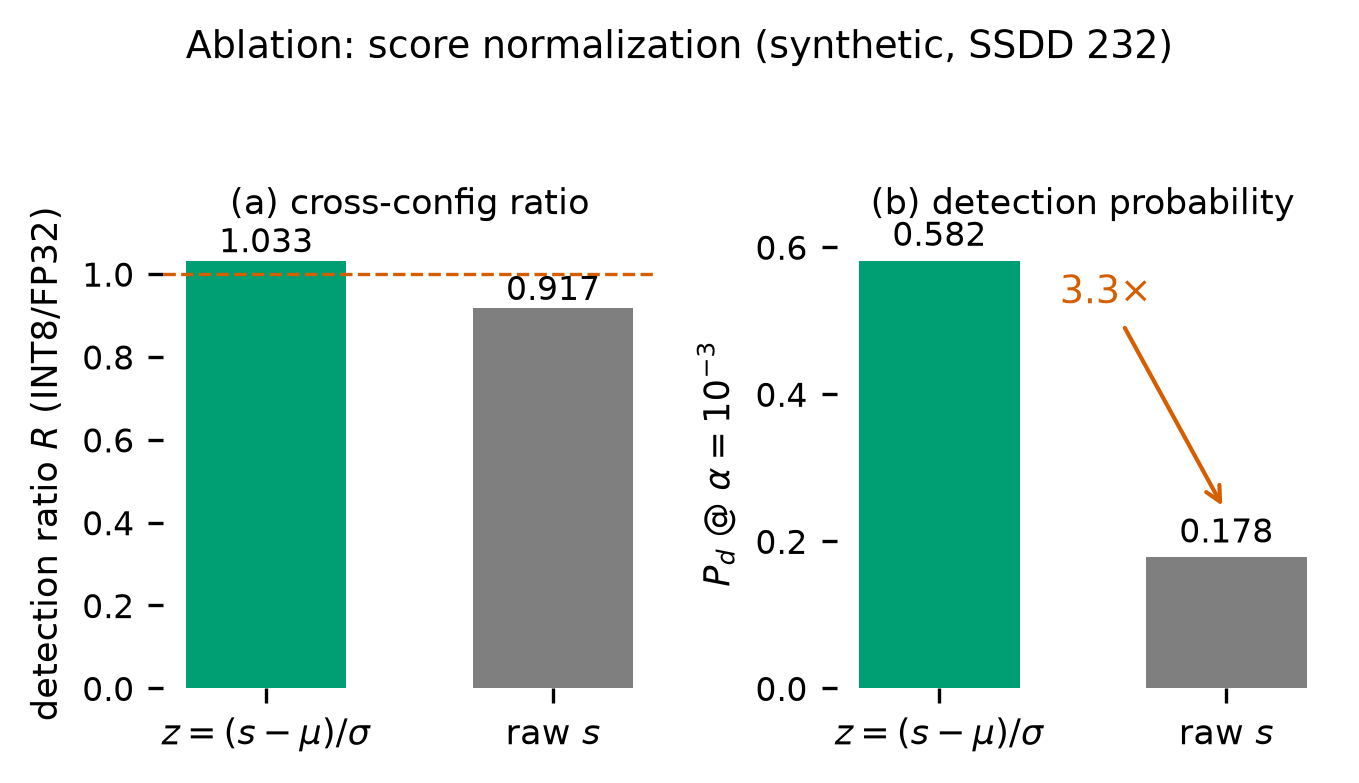
\includegraphics[width=11cm,height=\textheight,keepaspectratio,alt={Fig.27 方法核心设计消融（合成，SSDD 232）：(a) 分数归一化 h0------z=(s−μ)/σ vs 原始分数 s 直接阈值，R：1.033 vs 0.917，P\_d@α=1e-3：0.582 vs 0.178（3.3×）；(b) 校准集分层------分层（三海况）vs 只取平静，饱和率：0.5\% vs 9.0\%，R：0.881 vs 0.267。}]{sample_ablation_h0.png}
\caption*{Fig.27 方法核心设计消融（合成，SSDD 232）：(a) 分数归一化
h0------z=(s−μ)/σ vs 原始分数 s 直接阈值，R：1.033 vs
0.917，P\_d@α=1e-3：0.582 vs 0.178（3.3×）；(b)
校准集分层------分层（三海况）vs 只取平静，饱和率：0.5\% vs
9.0\%，R：0.881 vs 0.267。}
\end{figure}

\begin{figure}
\centering
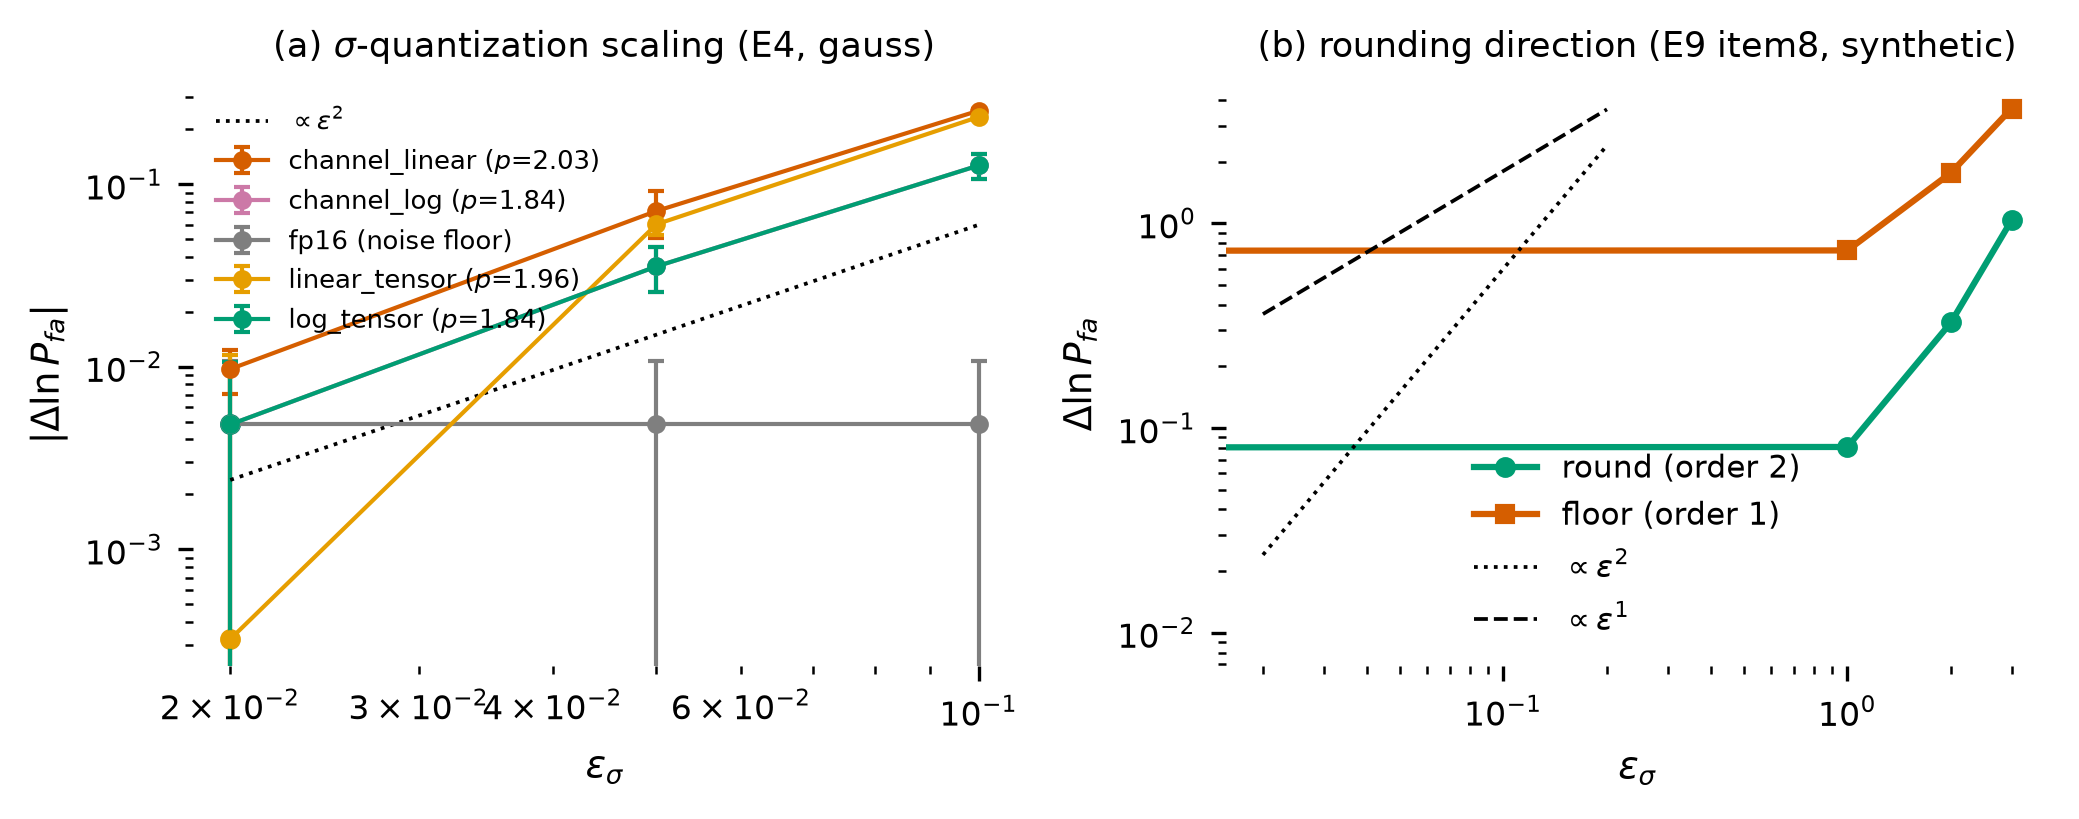
\includegraphics[width=11cm,height=\textheight,keepaspectratio,alt={Fig.28 σ 量化标度与取整方向（E4/E9 item8，合成 gauss）：(a) \textbar Δln P\_fa\textbar{} vs ε\_σ 的 log-log 拟合，斜率≈2；(b) round vs floor 取整方向的 Δln P\_fa 对照，round（指数 2.055）更符合 ε² 标度。}]{sample_ablation_scale.png}
\caption*{Fig.28 σ 量化标度与取整方向（E4/E9 item8，合成 gauss）：(a)
\textbar Δln P\_fa\textbar{} vs ε\_σ 的 log-log 拟合，斜率≈2；(b) round
vs floor 取整方向的 Δln P\_fa 对照，round（指数 2.055）更符合 ε² 标度。}
\end{figure}

Fig.29 将上述四项消融的关键对照数字汇总为一张 1×4
对比柱状图（各面板均以完整方法为参照）：\textbf{(a) 块抽样 keep
比}------keep 从 1.0 降至 0.0625 时 \(P_{fa}\) 从
\(1.59{\times}10^{-3}\) 单调抬升至 \(4.72{\times}10^{-3}\)（红色=偏离
\(2\alpha\) 容差），柱顶白字标注有效块数 \(n_{\mathrm{eff}}\) 从 49.8
压缩至 6.0------err 恶化与有限样本秩涨落同步；\textbf{(b)
标定样本量}------\(n\in\{16,64,128,200\}\) 的契约误差 mean±std
误差柱：n=128 处于平台最低段（0.0757），n=200 反升至 0.151、n=16 最差
0.0886 但方差最大；\textbf{(c) 全局 vs 逐场景标定}------\(P_{fa}\)
柱以契约误差入标签（0.201 vs 0.018）：逐场景重标定将 err
压缩一个量级，但需目标域数据；完整方法（逐场景模式）与全局模式的差距即''免数据搬运''要付出的标定成本；\textbf{(d)
校准集分层（合成）}------分层（三海况）INT8 \(P_{fa}\)
\(8.83{\times}10^{-4}\) 紧贴 FP32 参考线
\(1.00{\times}10^{-3}\)（\(R=0.881\)），只取平静海况则塌至
\(2.68{\times}10^{-4}\)（\(R=0.267\)，过度保守）------校准集覆盖度直接决定跨场景守约性。

\begin{figure}
\centering
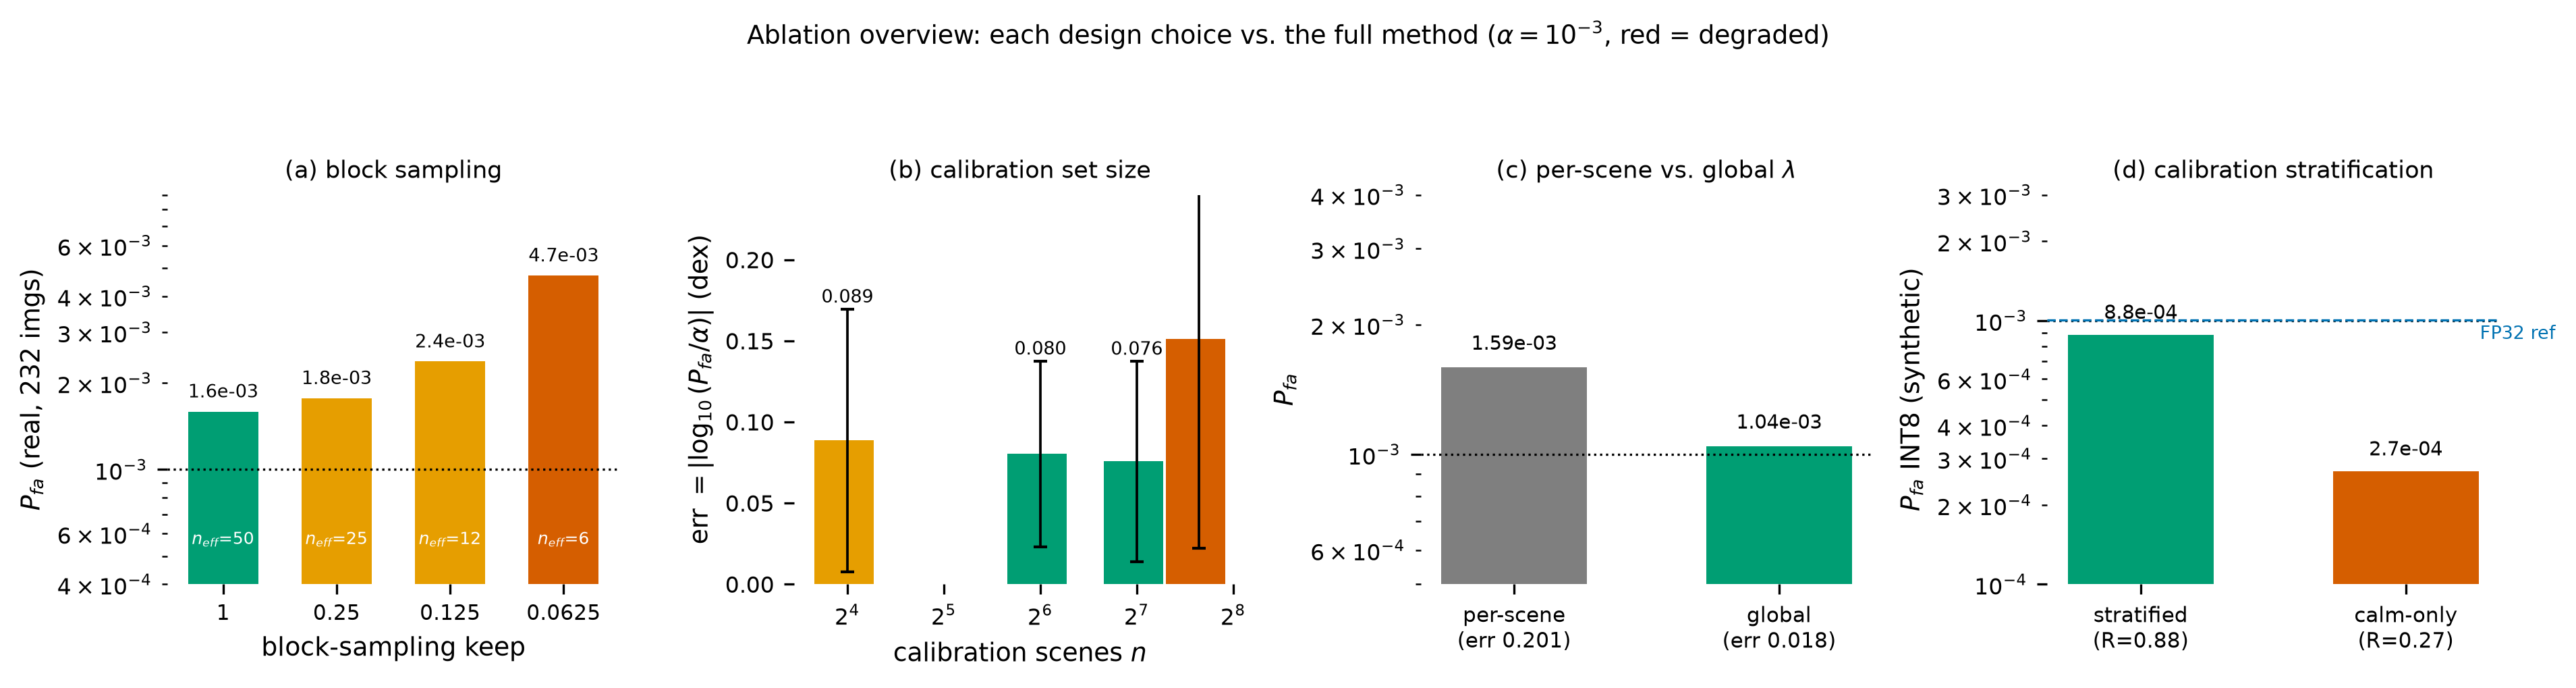
\includegraphics[width=16cm,height=\textheight,keepaspectratio,alt={Fig.29 消融配置 vs 完整方法对比汇总（1×4 面板，α=10\^{}-3，红色=超出 2α 容差）：(a) 块抽样 keep 比扫描（真实 232）P\_fa 柱 + n\_eff 白字；(b) 标定样本量 n∈\{16,64,128,200\} 误差柱（mean±std，reps=10）；(c) 全局（err 0.201）vs 逐场景（err 0.018）标定；(d) 校准集分层（合成）：分层 INT8 P\_fa 8.83e-4（R=0.881）贴 FP32 参考线，只取平静塌至 2.68e-4（R=0.267）。}]{sample_ablation_bar.png}
\caption*{Fig.29 消融配置 vs 完整方法对比汇总（1×4
面板，α=10\^{}-3，红色=超出 2α 容差）：(a) 块抽样 keep 比扫描（真实
232）P\_fa 柱 + n\_eff 白字；(b) 标定样本量 n∈\{16,64,128,200\}
误差柱（mean±std，reps=10）；(c) 全局（err 0.201）vs 逐场景（err
0.018）标定；(d) 校准集分层（合成）：分层 INT8 P\_fa
8.83e-4（R=0.881）贴 FP32 参考线，只取平静塌至 2.68e-4（R=0.267）。}
\end{figure}

Fig.35 把 E9 消融中\textbf{最能支撑方法设计的三个对照}集中为一张 2×2
对比图（数字与 Table 10c/10e/10f 同源）：\textbf{(a) 分数归一化
\(h_0\)（item 6）}------含 \(h_0\)（\(z=(s-\mu)/\sigma\)）与去除
\(h_0\)（原始分数 \(s\) 直接阈值）的 \(R\) 与 \(P_d@10^{-3}\)
双柱并列：\(R\) 1.033 vs 0.917、\(P_d\) 0.582 vs
0.178，两指标同向崩塌------归一化同时是''跨配置可比''（E5
搬运前提）与''检测力''的必要件；\textbf{(b) 校准集分层（item
7）双轴对照}------饱和率（左轴，紫）0.5\% vs 9.0\% 与 INT8
\(P_{fa}\)（右轴，棕，\(\times10^{-4}\)）8.8 vs
2.7：只取平静海况校准时饱和与过度保守（\(P_{fa}\) 塌至
0.27\(\alpha\)）同时出现，饱和率与守约性并非独立症状而是同一覆盖度缺陷的两面；\textbf{(c)
分层消融的 \(R\) 对比}------分层 0.881 落在 \(R=1\pm20\%\)
契约带内、只取平静 0.267 远离带宽，\(\pm20\%\) 阴影带即 §4.1.4
的验收容差；\textbf{(d) 全局 vs 逐场景标定误差（真实数据，item
5）}------err 0.0185 vs 0.2014（log 轴）相差一个量级，0.05 dex
参考线（有限样本噪声底）下全局模式的 in-sample 优势清晰可见（口径注见表
10c），而 \(\Delta P_d\) 仅
0.0035------精度优势不以牺牲检测力为代价。Fig.27--29
给出各单项的曲线细节，Fig.35
提供三项关键消融的并排总览，便于读者一图核对''每个设计选择拿掉后塌多少''。

\begin{figure}
\centering
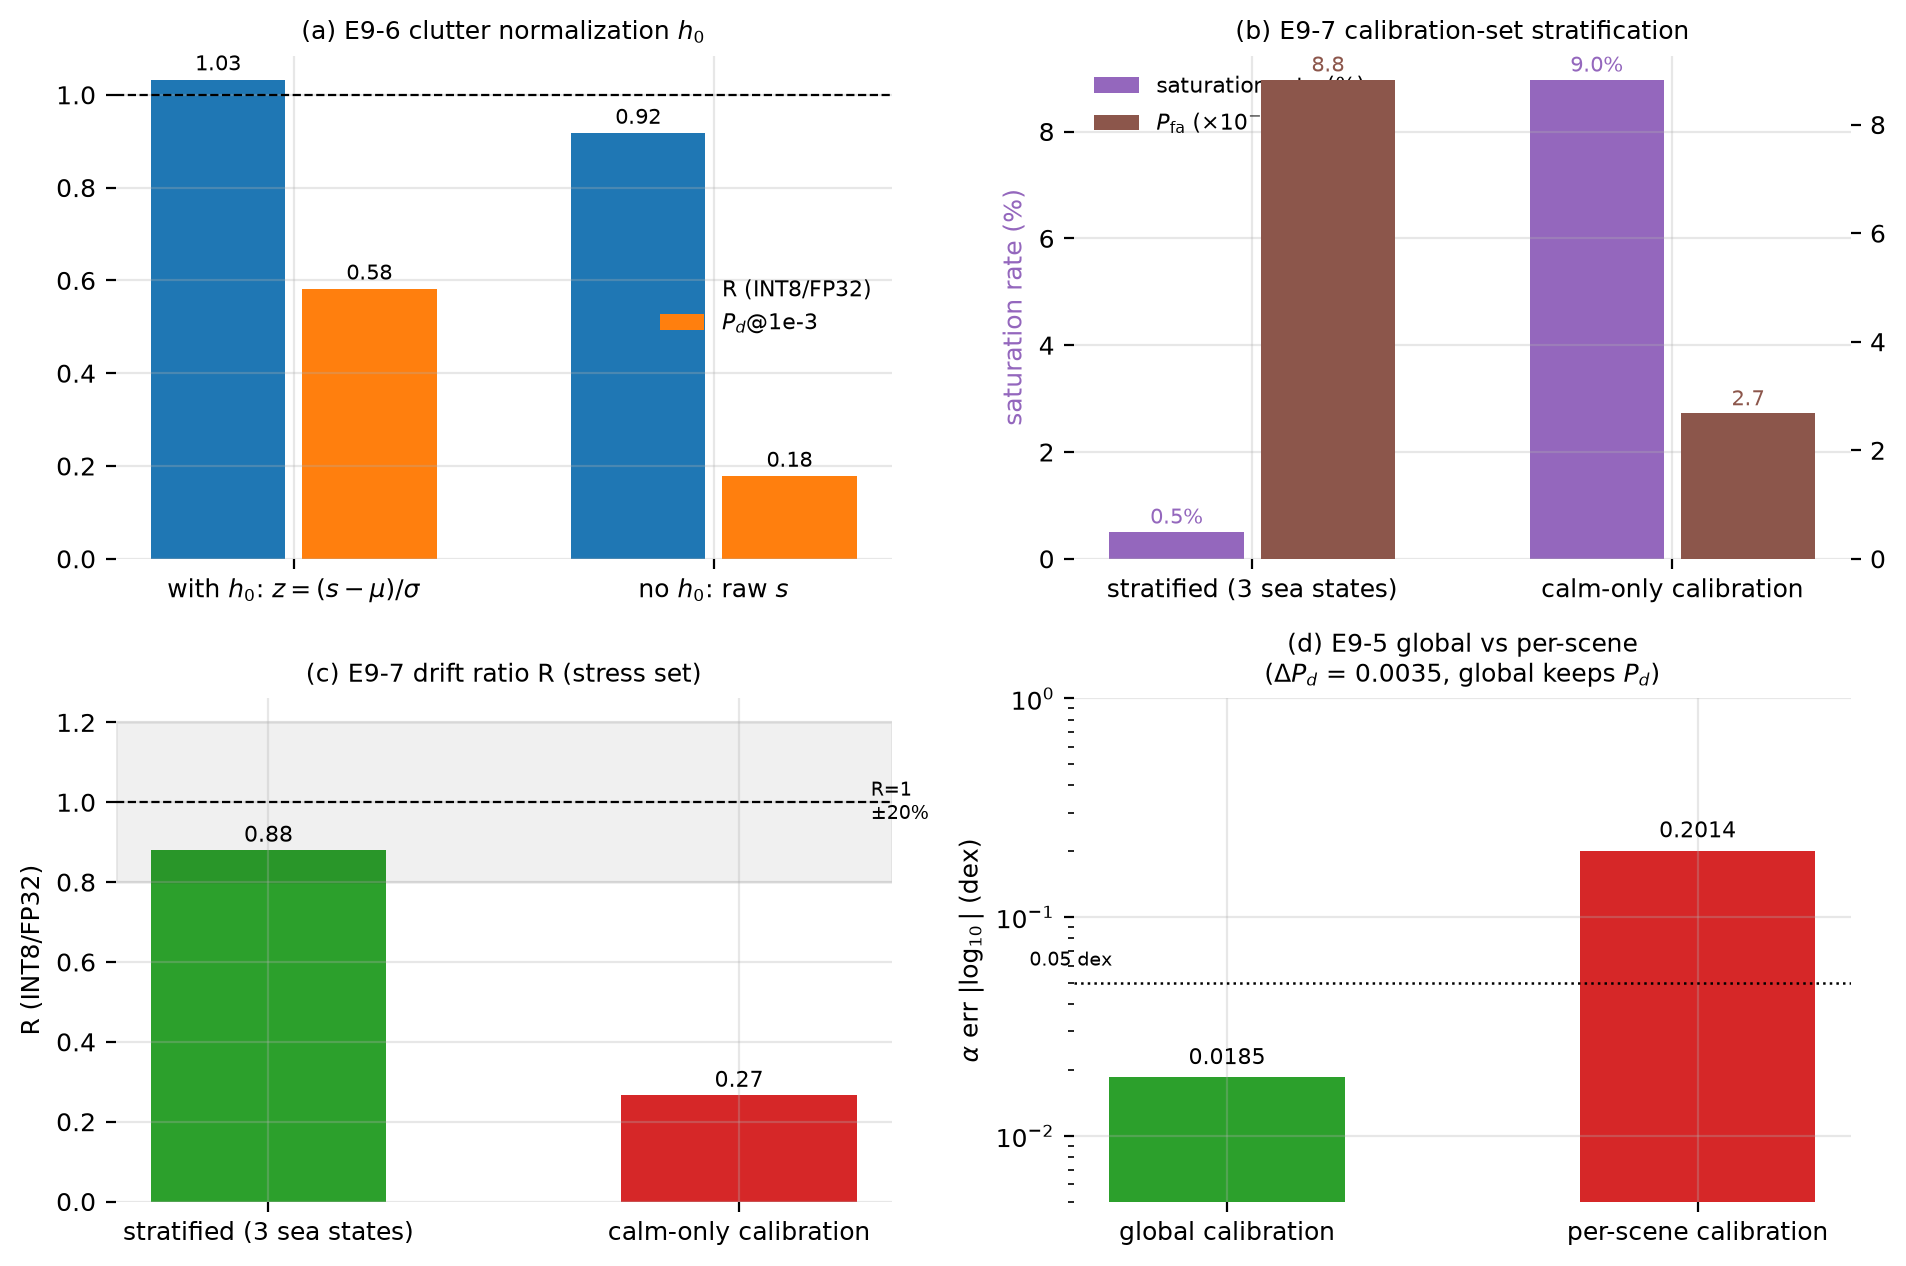
\includegraphics[width=16cm,height=\textheight,keepaspectratio,alt={Fig.35 E9 消融关键对照汇总（2×2，数字与 Table 10c/10e/10f 同源）：(a) h0 归一化------R 1.033 vs 0.917、P\_d@1e-3 0.582 vs 0.178；(b) 校准集分层双轴------饱和率 0.5\% vs 9.0\%（左轴）、INT8 P\_fa 8.8e-4 vs 2.7e-4（右轴）；(c) R 对比------分层 0.881 在 ±20\% 契约带内、只取平静 0.267 塌出带宽；(d) 全局 vs 逐场景标定 err 0.0185 vs 0.2014（log 轴，真实数据，ΔP\_d=0.0035）。}]{fig32_ablation_summary.png}
\caption*{Fig.35 E9 消融关键对照汇总（2×2，数字与 Table 10c/10e/10f
同源）：(a) h0 归一化------R 1.033 vs 0.917、P\_d@1e-3 0.582 vs
0.178；(b) 校准集分层双轴------饱和率 0.5\% vs 9.0\%（左轴）、INT8 P\_fa
8.8e-4 vs 2.7e-4（右轴）；(c) R 对比------分层 0.881 在 ±20\%
契约带内、只取平静 0.267 塌出带宽；(d) 全局 vs 逐场景标定 err 0.0185 vs
0.2014（log 轴，真实数据，ΔP\_d=0.0035）。}
\end{figure}

\begin{center}\rule{0.5\linewidth}{0.5pt}\end{center}

\subsection{定性可视化与场景类型分析（远洋/近岸 /
Fig.30--Fig.38）}\label{ux5b9aux6027ux53efux89c6ux5316ux4e0eux573aux666fux7c7bux578bux5206ux6790ux8fdcux6d0bux8fd1ux5cb8-fig.30fig.38}

\textbf{动机与分类协议。} E7
的负载解耦证据按海况分桶给出；本节补充第二个人工可判读的难度维度------\textbf{远洋（offshore）vs
近岸（nearshore）}：近岸场景含海岸线与陆地，检测器分数图上出现大块强响应杂波，是误警与候选负载的另一压力源。本地
SSDD 发布未保留官方 inshore/offshore
标注，我们采用可复现的两步协议重新划分 232
张测试图：①计算陆地各向异性分数
coast\_score（图像行均值与列均值的标准差之和，陆地大块亮/暗结构产生强各向异性）；②按分数排序生成缩略拼版人工确认。TOP-40（coast\_score
中位数 41.9）均含明显海岸线/陆地，rank 49--96 复核为开阔海面，故取
TOP-40 为近岸、其余 192 张为远洋（划分资产
\texttt{code/results/e7/e7\_scene\_type.csv}）。交叉核对：近岸集中于
medium/rough 海况桶（4/36/0），远洋为 31/138/23，两维度（海况 ×
场景类型）近似正交，可分别归因。

\textbf{定性结果（Fig.30 / Fig.31）。} Fig.30 与 Fig.31
分别给出近岸（001111/001091/001159）与远洋（000739/001149/001121）典型帧的检测框可视化（绿
= GT，橙 = INT8 检出，上下两行分别为 calmA / roughB 校准集）：INT8
在近岸陆地杂波下仍能检出主要目标，但可观察到校准集差异对近岸帧检出框的影响大于远洋帧------与
E5 设置 1（换校准集搬运）的定量结论互为印证。
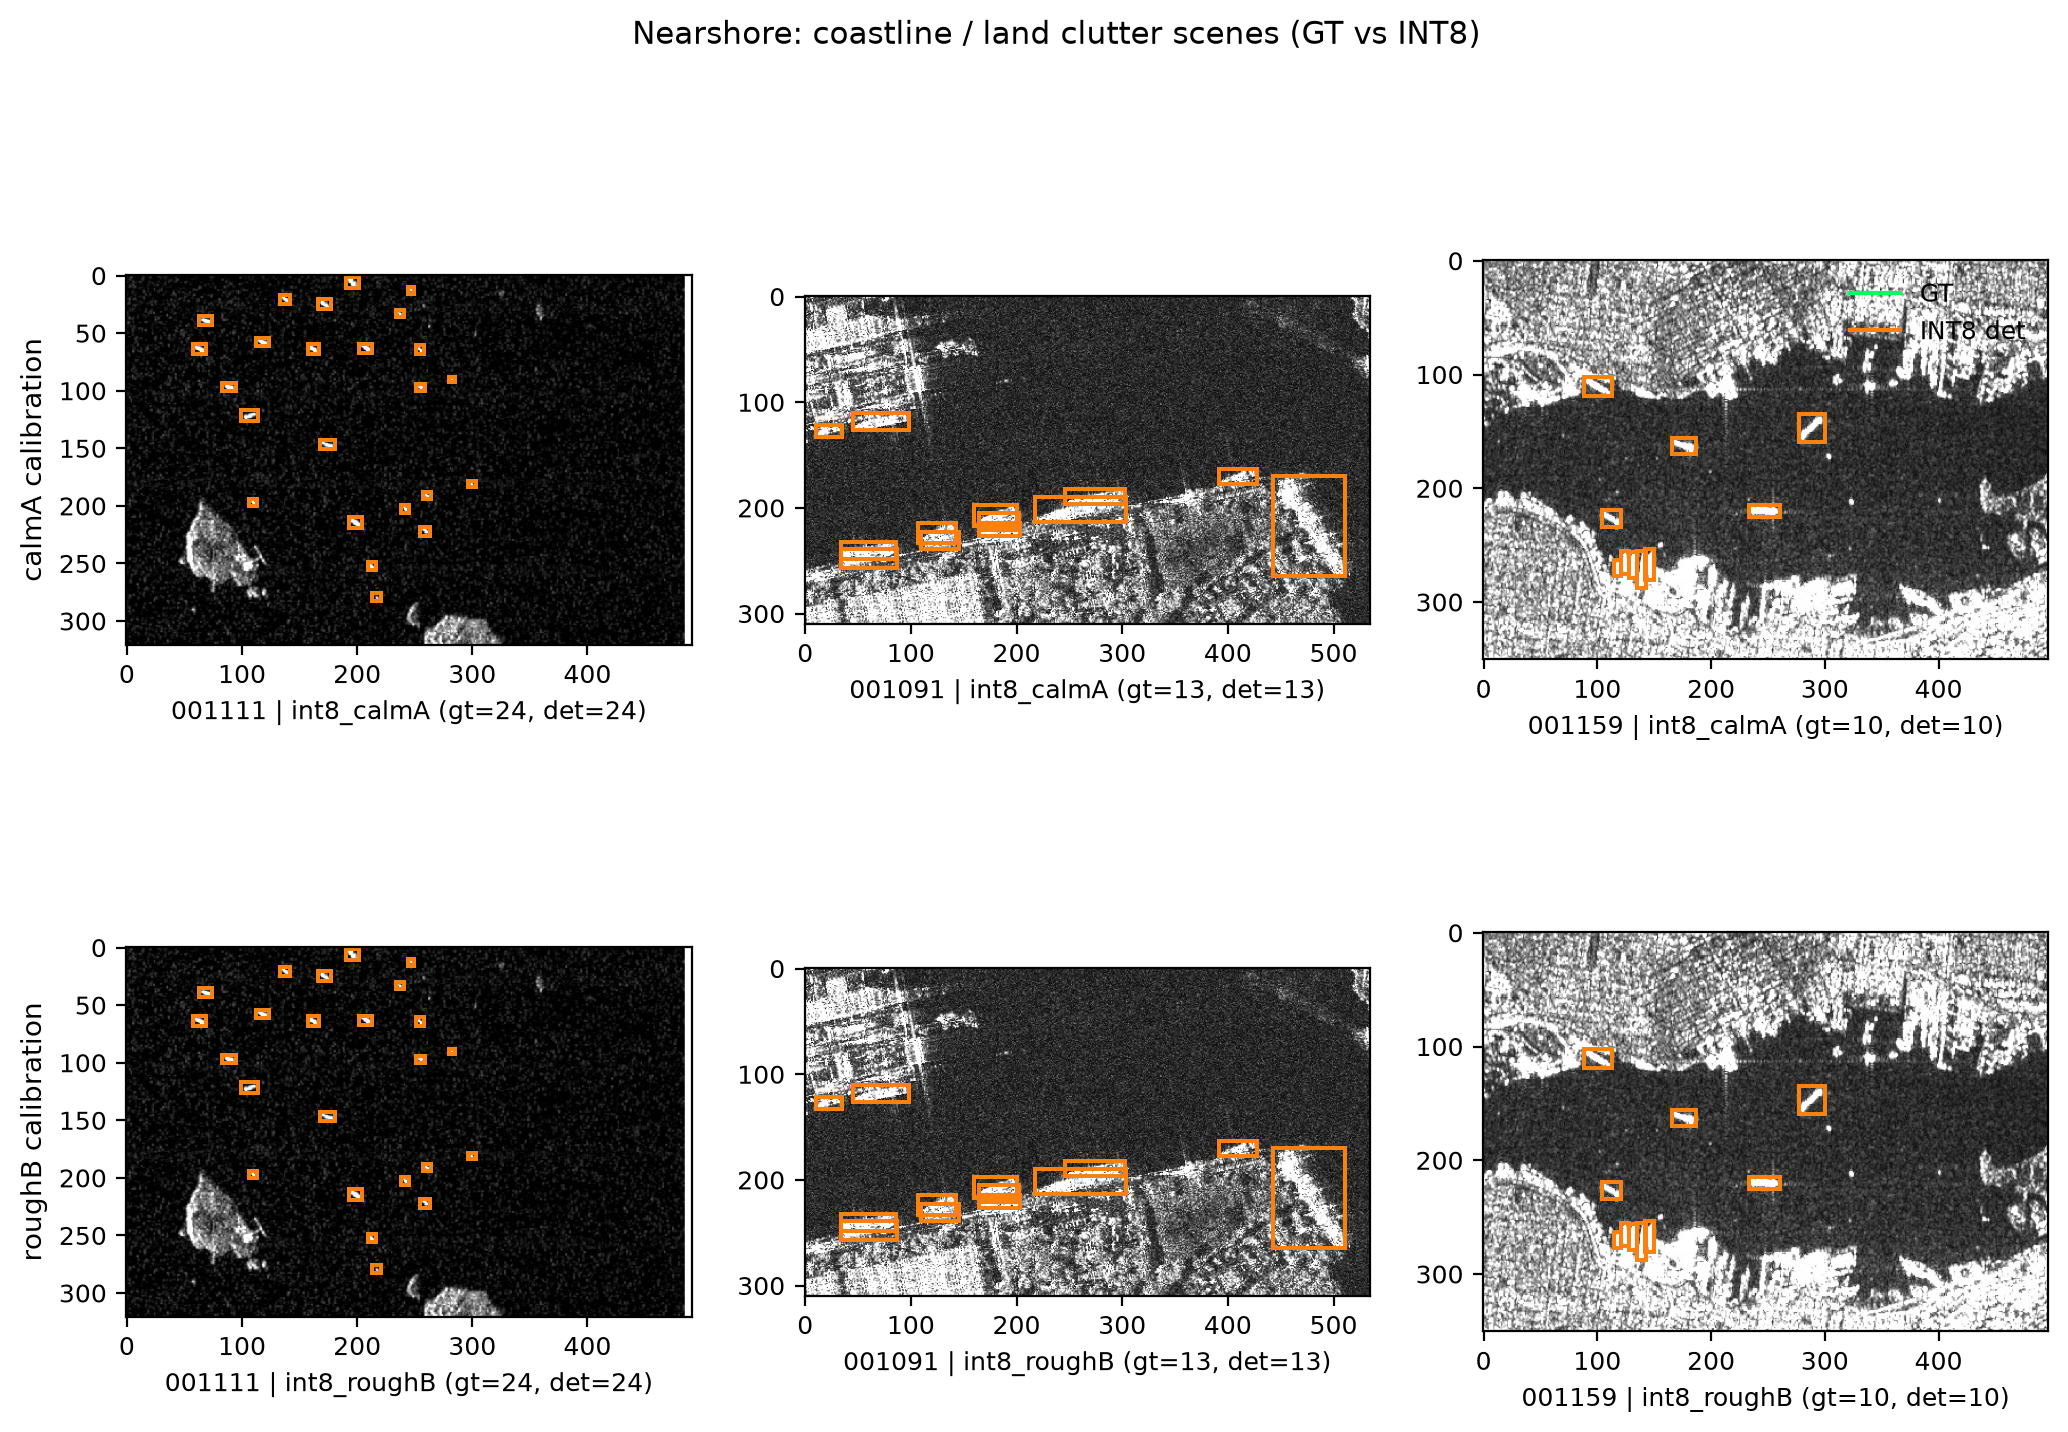
\includegraphics[width=16cm,height=\textheight,keepaspectratio,alt={Fig.30 近岸（海岸线/陆地杂波）典型帧检测可视化：绿 = GT，橙 = INT8 检出；上/下两行分别为 calmA / roughB 校准集。}]{fig27_nearshore_gallery.png}

\begin{figure}
\centering
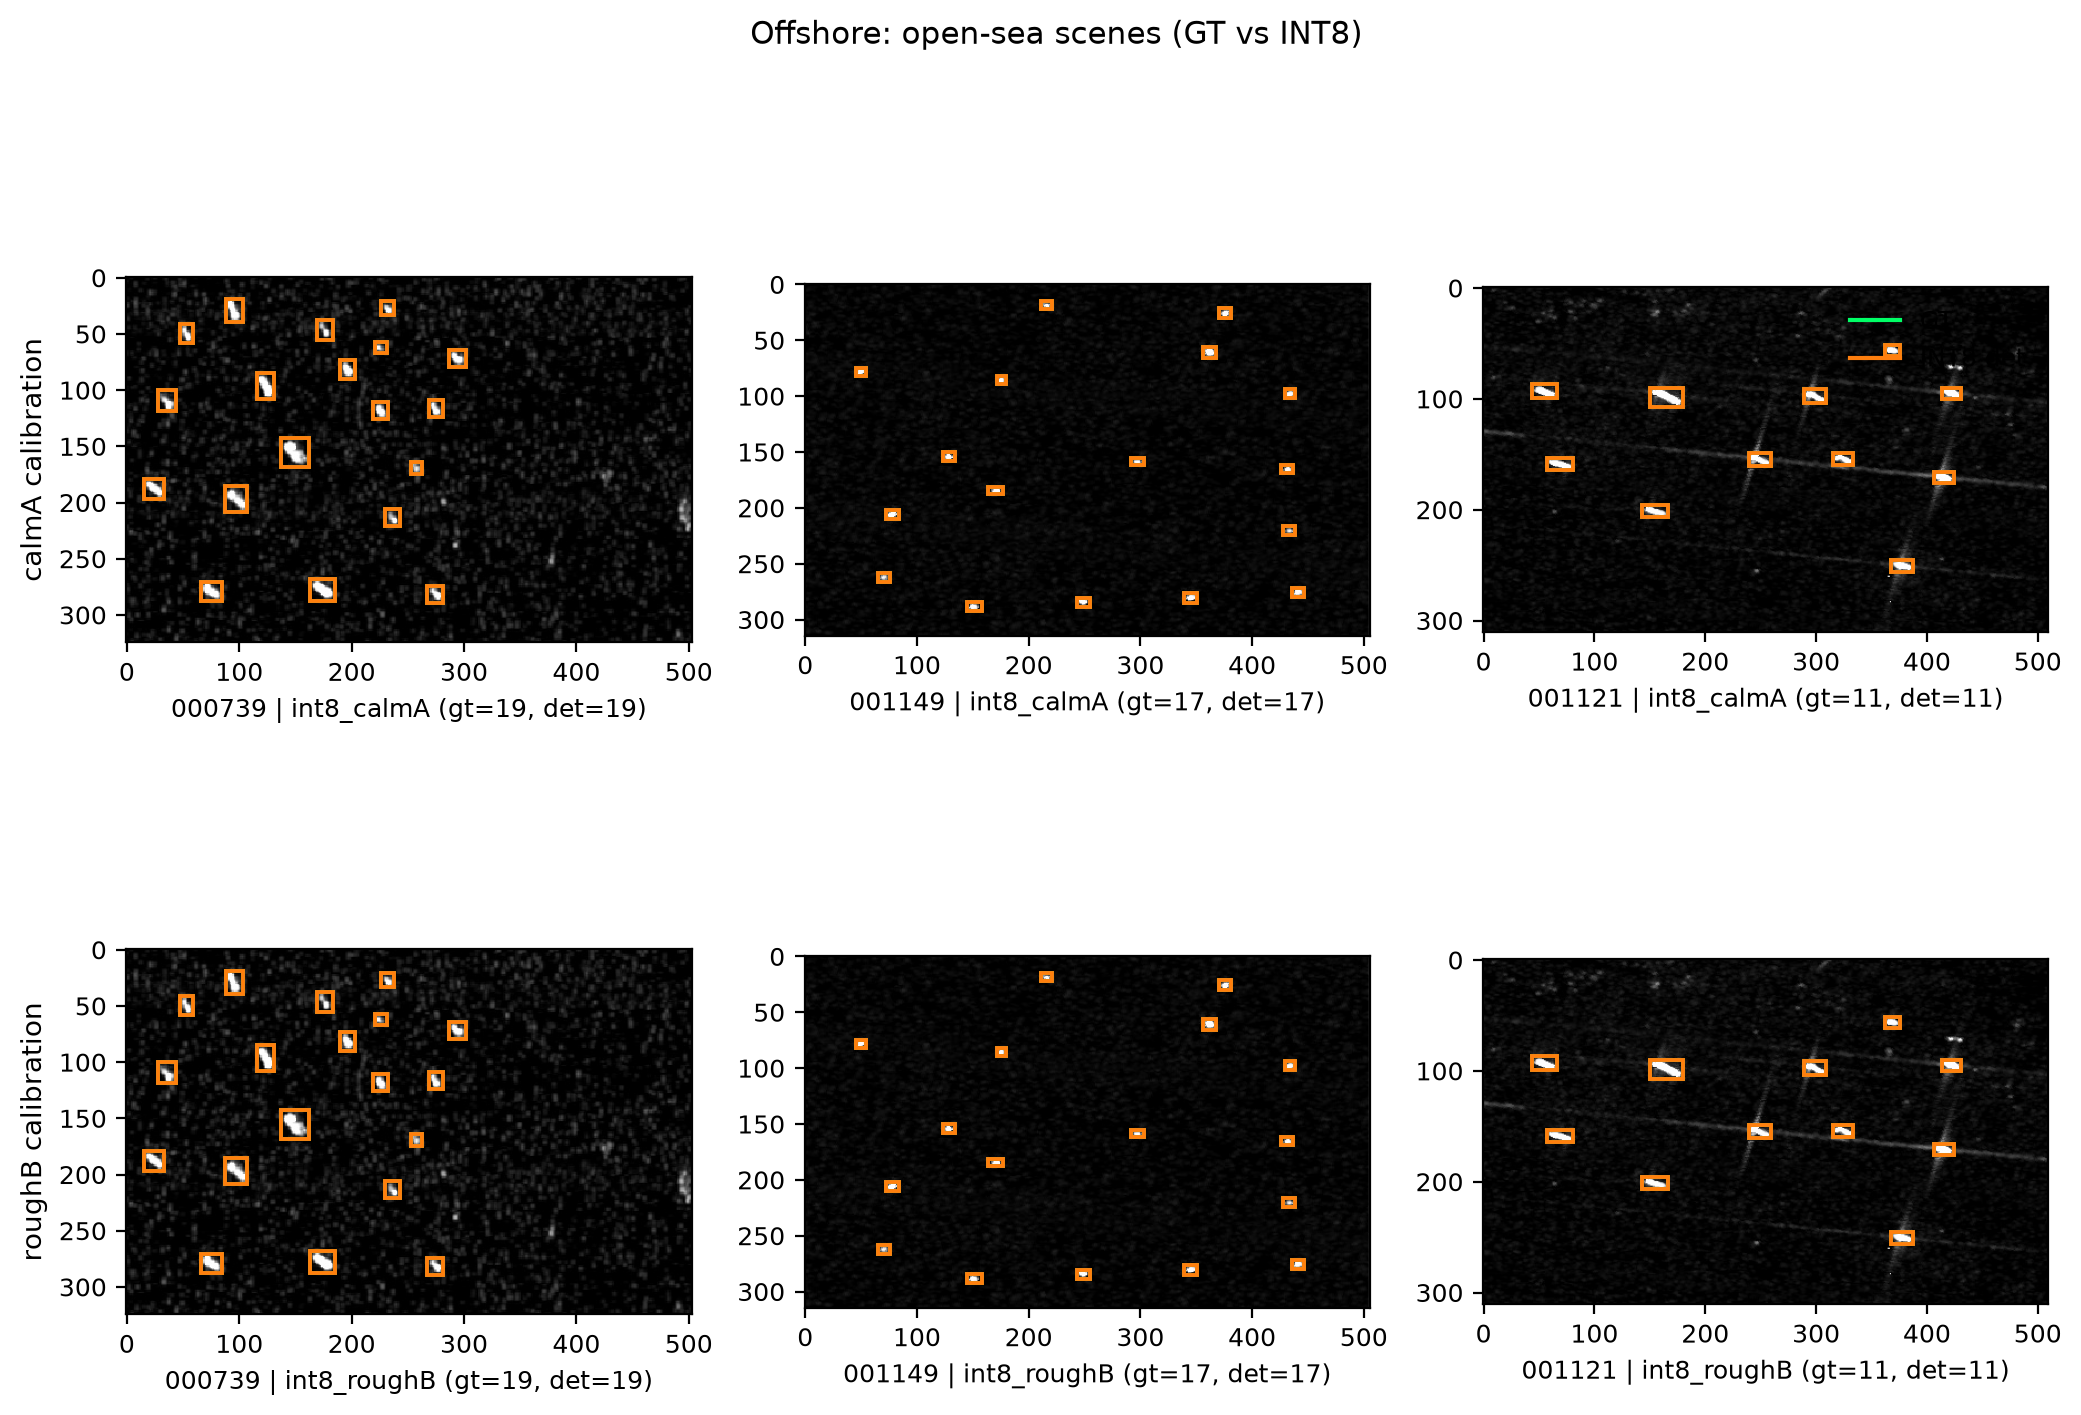
\includegraphics[width=16cm,height=\textheight,keepaspectratio,alt={Fig.31 远洋（开阔海域）典型帧检测可视化，格式同 Fig.30。}]{fig28_offshore_gallery.png}
\caption*{Fig.31 远洋（开阔海域）典型帧检测可视化，格式同 Fig.30。}
\end{figure}

\textbf{分数图证据（Fig.32）。} Fig.32 将 P3 objectness 热力图（去
letterbox 对齐，alpha
混合）叠加于原始图像：近岸帧在陆地/海岸线区域出现大面积高响应，而船位响应与陆地响应幅值可比------这正是逐帧
\(P_{fa}\)
在近岸子集违约率更高的机理来源；远洋帧高响应区基本只出现在船位及其尾迹。
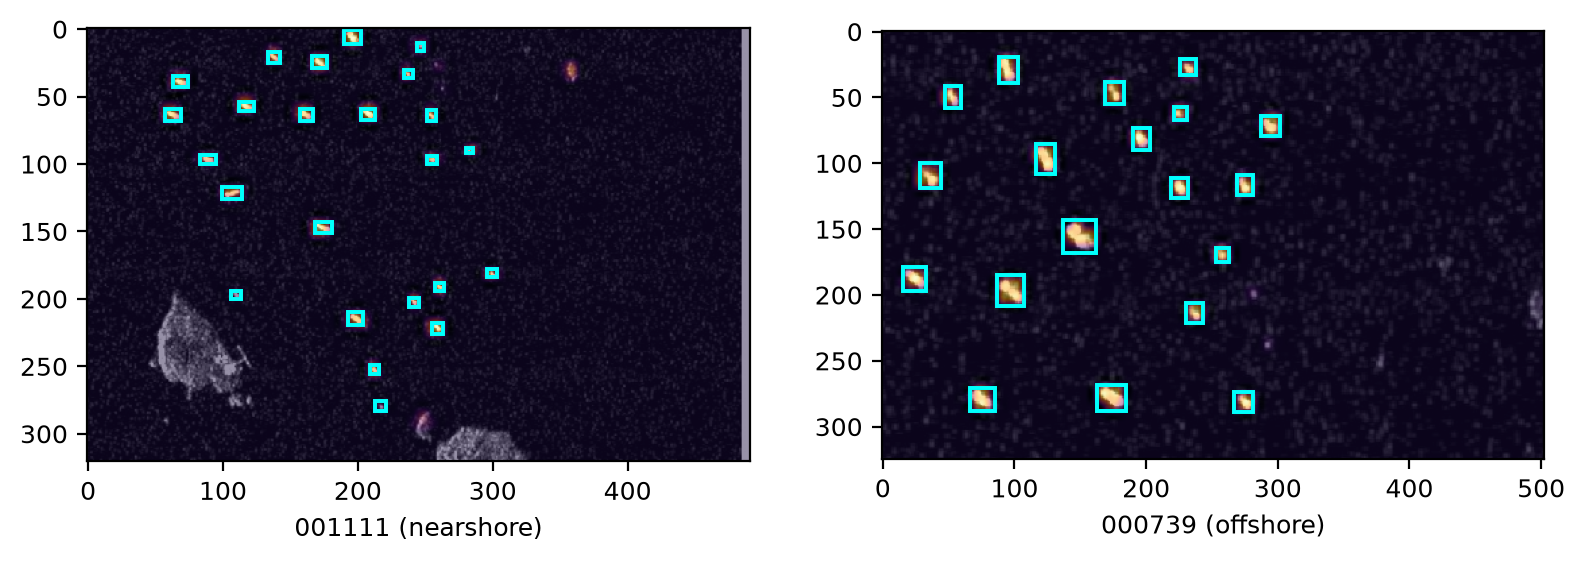
\includegraphics[width=16cm,height=\textheight,keepaspectratio,alt={Fig.32 P3 objectness 热力图叠加底图（去 letterbox 对齐，alpha 混合）：近岸帧（左）陆地/海岸线区域大面积高响应，远洋帧（右）高响应区基本只出现在船位及尾迹。}]{fig29_scene_heatmap_overlay.png}

\textbf{定量复核（Fig.33 与 Table 8b 口径一致）。} Fig.33
给出三面板证据：(a) 逐帧 \(P_{fa}/\alpha\)
按场景类型着色------INT8-全局运行点在近岸子集 \(>2\alpha\) 违约率
\textbf{20.0\%}（8/40），约为远洋子集
\textbf{9.9\%}（19/192）的两倍，\(>5\alpha\) 分别为 2.5\%/1.6\%；(b)
候选负载箱线------近岸 p90 = 20.5 vs 远洋 15.9（中位数 5 vs
6，近岸尾部更重）；(c) 海况 × 场景类型构成。\textbf{QCert
运行点在两个子集上均恒为 1.07\(\alpha\)、零违约}------把 §4.9
的''海况耦合''证据扩展到''场景类型耦合''维度：无论难度来自海况还是陆地杂波，分位数校准阈值都保持契约，而全局阈值在两类压力下都出现尾部违约。
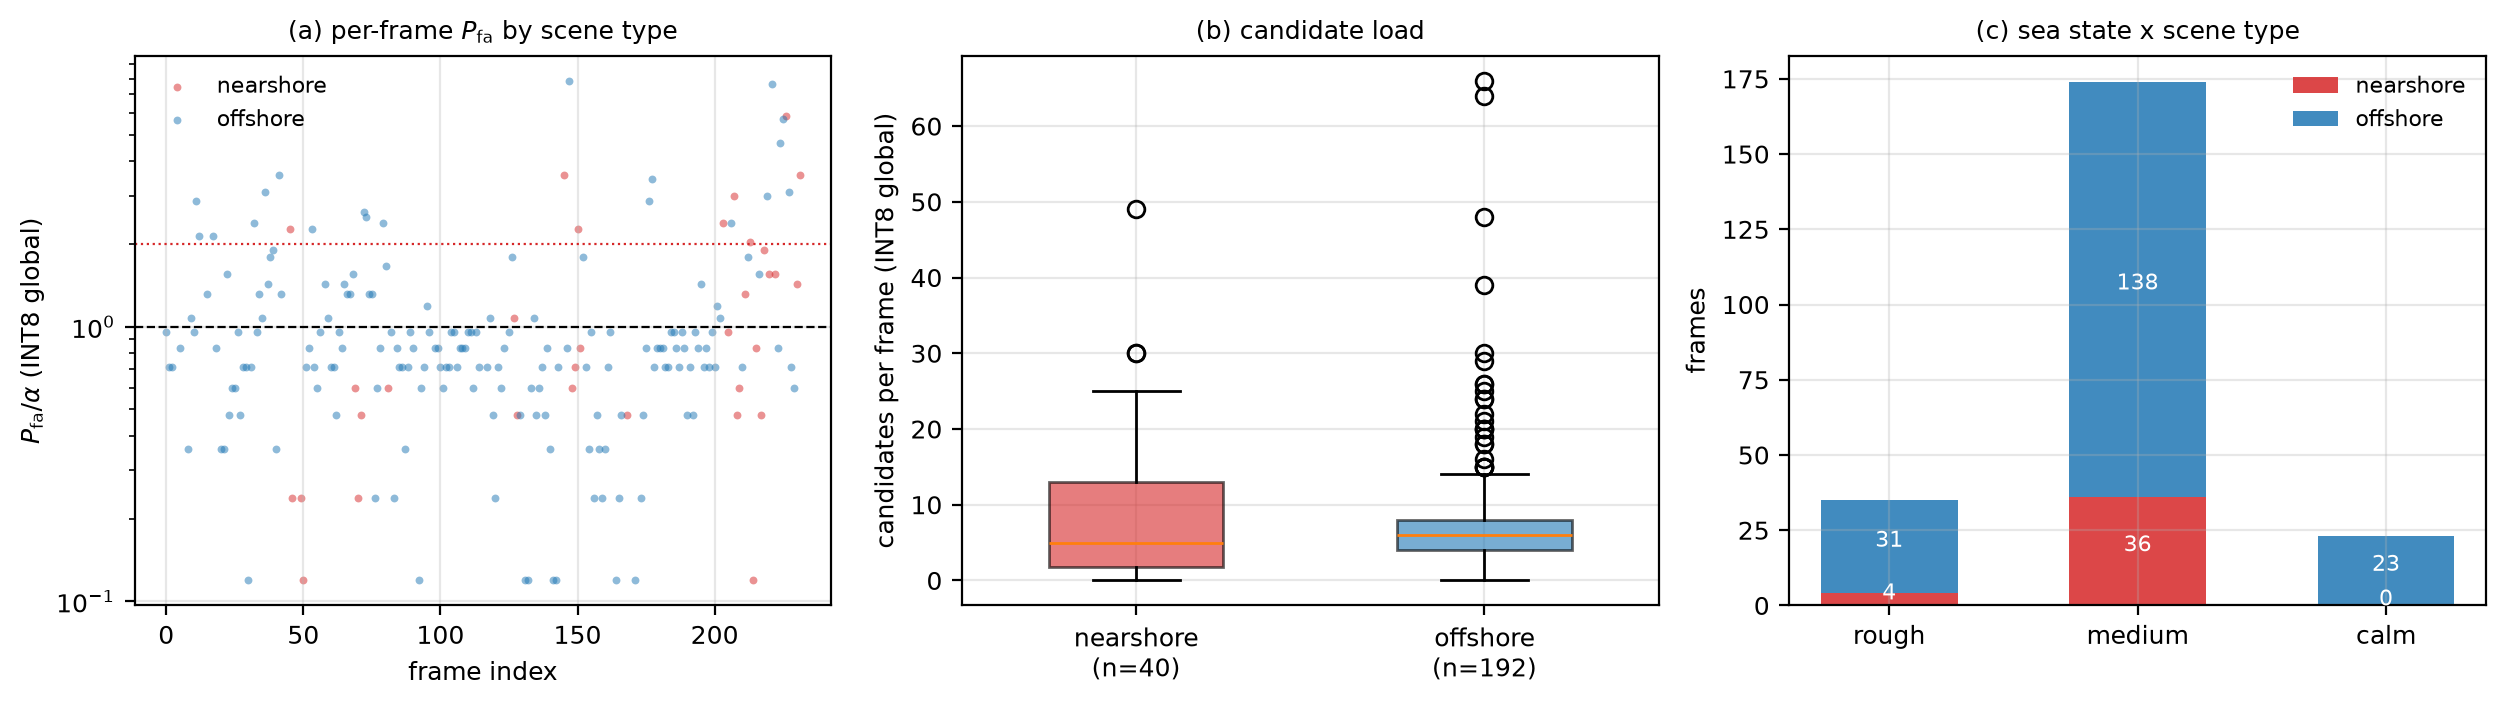
\includegraphics[width=16cm,height=\textheight,keepaspectratio,alt={Fig.33 场景类型定量复核：(a) 逐帧 P\_\{\textbackslash rm fa\}/\textbackslash alpha 按远洋/近岸着色（INT8-全局，近岸 \textgreater2\textbackslash alpha 违约 20.0\% vs 远洋 9.9\%）；(b) 候选负载箱线（近岸 p90=20.5 vs 远洋 15.9）；(c) 海况 × 场景类型构成。QCert 在两个子集均恒 1.07\textbackslash alpha、零违约。}]{fig30_pfa_scene_type.png}

\begin{quote}
注：近岸/远洋划分系人工确认的可复现协议产物（非 SSDD 官方标注），样本量
\(n_{nearshore}=40\)，\(>5\alpha\) 违约仅 1 例，尾部结论以 \(>2\alpha\)
口径为主。
\end{quote}

\textbf{分布级对比（Fig.34）。} Fig.33 的散点/箱线给出尾部点证据，Fig.34
进一步给出\textbf{四个分布级 ECDF/直方图对比}：\textbf{(a)
INT8-全局运行点的逐帧 \(P_{fa}/\alpha\)
ECDF}------近岸曲线（红）整体右移，\(>2\alpha\) 违约 20.0\% vs 远洋
9.9\% 在图上表现为 ECDF 末端落在红色虚线右侧的余量差；\textbf{(b)
INT8-QCert 运行点同口径 ECDF}------两个子集的曲线几乎重合且全部收敛于
\(1.07\alpha\)（黑虚线右侧极窄区间），分布级直接呈现''分位数校准把两类场景拉回同一守约分布''；\textbf{(c)
候选负载 ECDF}------近岸曲线在全分位段右移（中位数 5 vs 6
之外，上分位差距更明显），p90 = 20.5 vs 15.9；\textbf{(d) coast\_score
分布直方图}------近岸（红）与远洋（蓝）近似双峰分离，TOP-40
分界线（29.3）落在两峰之间的谷地，直观解释了该划分协议为何只需一个标量阈值。

\begin{figure}
\centering
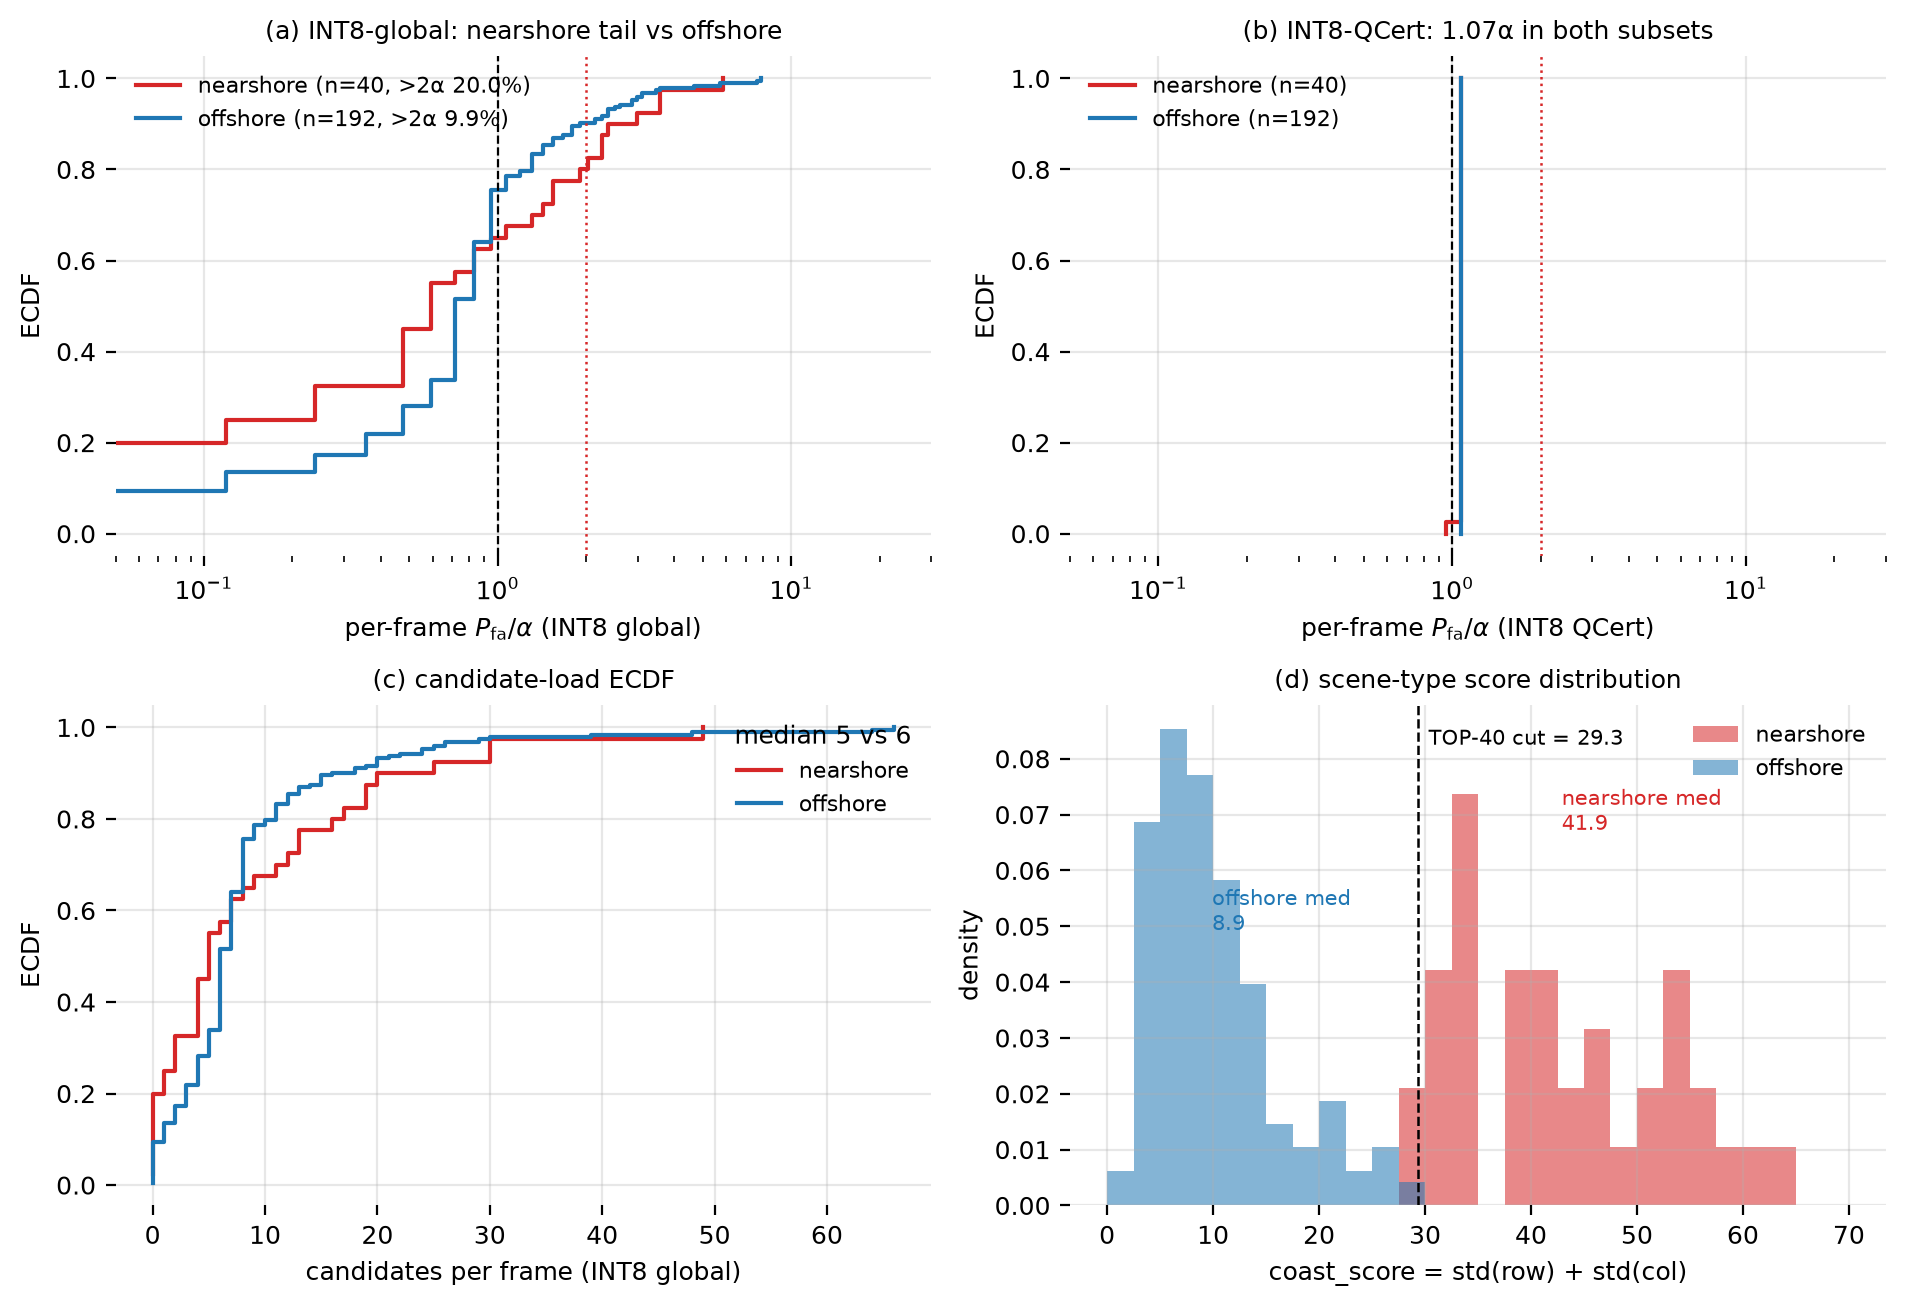
\includegraphics[width=16cm,height=\textheight,keepaspectratio,alt={Fig.34 近岸/远洋分布级对比（2×2，E7 口径 232 帧）：(a) INT8-全局逐帧 P\_fa/α ECDF（近岸 \textgreater2α 违约 20.0\% vs 远洋 9.9\%）；(b) INT8-QCert 同口径 ECDF------双子集重合且恒 1.07α；(c) 候选负载 ECDF（中位数 5 vs 6，p90 20.5 vs 15.9）；(d) coast\_score 分布直方图与 TOP-40 分界线（近岸中位 41.9 vs 远洋 8.9）。}]{fig31_scene_pfa_ecdf.png}
\caption*{Fig.34 近岸/远洋分布级对比（2×2，E7 口径 232 帧）：(a)
INT8-全局逐帧 P\_fa/α ECDF（近岸 \textgreater2α 违约 20.0\% vs 远洋
9.9\%）；(b) INT8-QCert 同口径 ECDF------双子集重合且恒 1.07α；(c)
候选负载 ECDF（中位数 5 vs 6，p90 20.5 vs 15.9）；(d) coast\_score
分布直方图与 TOP-40 分界线（近岸中位 41.9 vs 远洋 8.9）。}
\end{figure}

\textbf{逐帧对照 gallery（Fig.37）。} Fig.30/31
按场景类型各给一组典型帧，Fig.37
把两类场景\textbf{并排放入同一图内直接对照}，并在每帧标题标注该帧的实测
\(P_{fa}/\alpha\)（INT8-全局）与候选数：上排近岸（001131：5.83\(\alpha\)、cand=49；001159：3.57\(\alpha\)、cand=30；001039：2.98\(\alpha\)、cand=25；001111：1.55\(\alpha\)、cand=13）------陆地/海岸线杂波下
\(P_{fa}\) 普遍越线、候选负载为远洋合规帧的 10
倍量级；下排远洋（001149：0.60\(\alpha\)、cand=5；000109：0.36\(\alpha\)；000249：0.24\(\alpha\)）大多低于
\(\alpha\)，但
\textbf{000739（7.86\(\alpha\)、cand=66）作为远洋尾部离群帧}同样出现高违约------说明远洋
9.9\% 的尾部违约并非陆地杂波所致，而是强船迹/尾迹类强响应（机理见 Fig.38
右下图）。两类场景的检出框（橙）与 GT（绿）均贴合，\(P_{fa}\)
差异不来自漏检而来自背景响应结构。

\begin{figure}
\centering
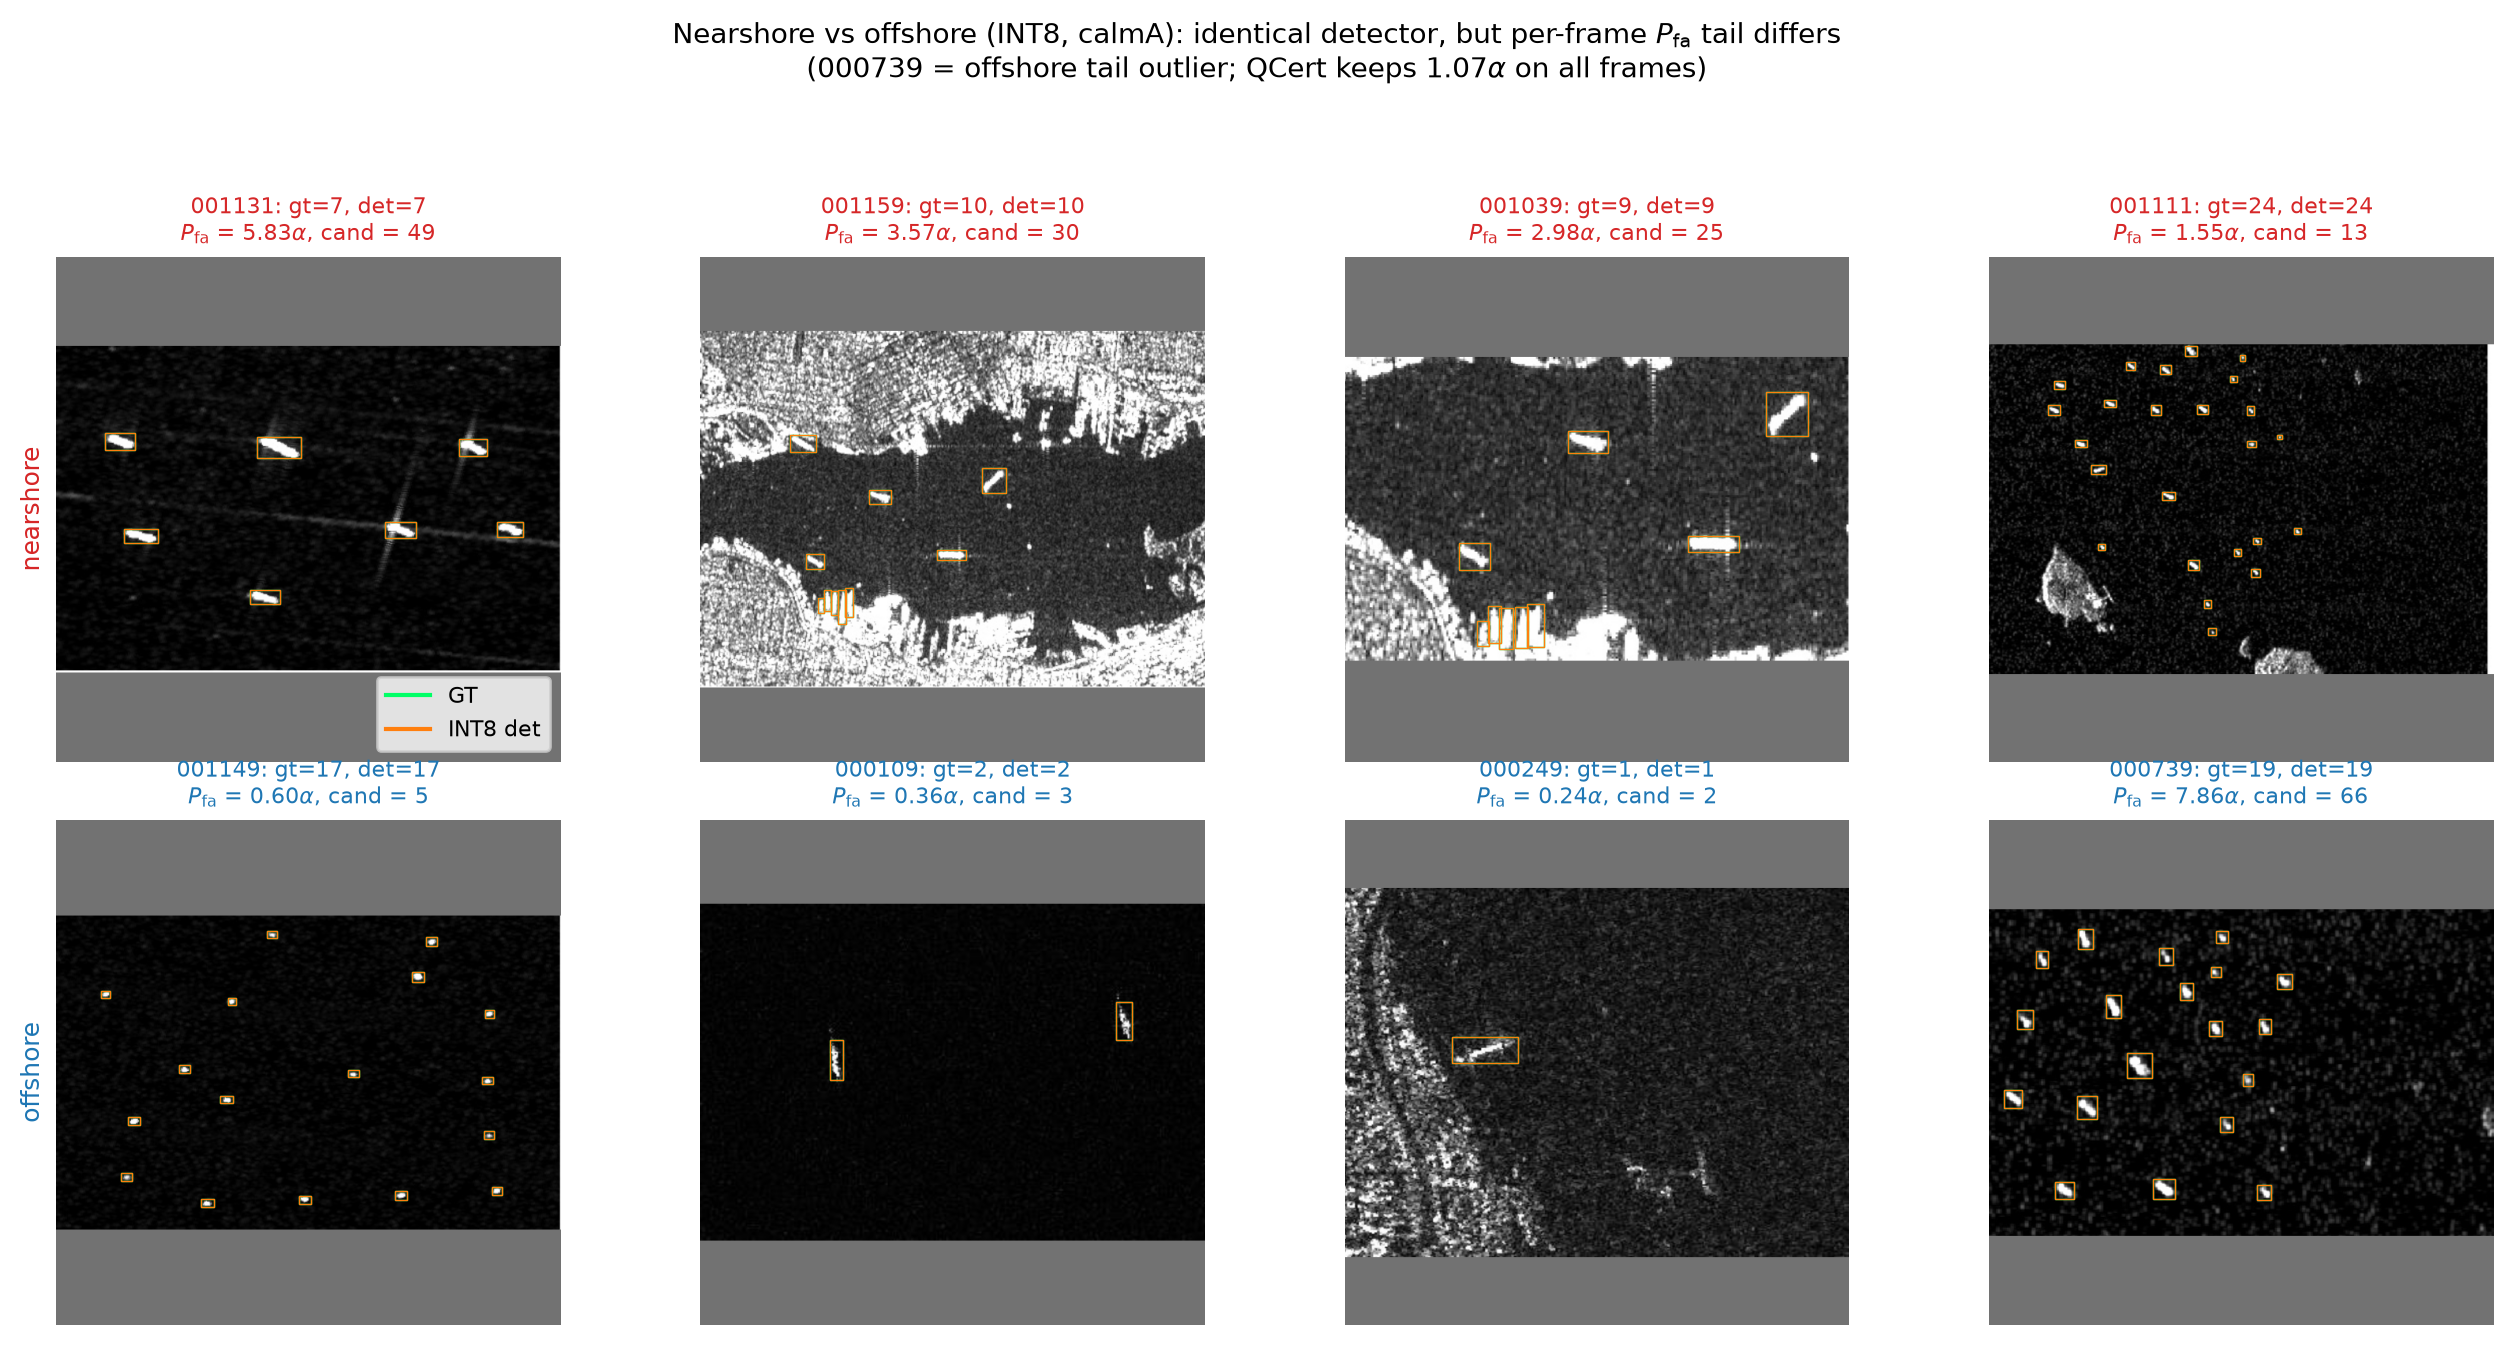
\includegraphics[width=16cm,height=\textheight,keepaspectratio,alt={Fig.37 近岸/远洋逐帧并排对照 gallery（INT8，calmA，2×4）：上排近岸（001131/001159/001039/001111，P\_fa=5.83/3.57/2.98/1.55α，cand=49/30/25/13），下排远洋（001149/000109/000249/000739，P\_fa=0.60/0.36/0.24/7.86α，cand=5/3/2/66------000739 为远洋尾部离群帧）。绿=GT，橙=INT8 检出；每帧标题含实测逐帧 P\_fa/α 与候选数。}]{fig34_scene_gallery_compare.png}
\caption*{Fig.37 近岸/远洋逐帧并排对照
gallery（INT8，calmA，2×4）：上排近岸（001131/001159/001039/001111，P\_fa=5.83/3.57/2.98/1.55α，cand=49/30/25/13），下排远洋（001149/000109/000249/000739，P\_fa=0.60/0.36/0.24/7.86α，cand=5/3/2/66------000739
为远洋尾部离群帧）。绿=GT，橙=INT8 检出；每帧标题含实测逐帧 P\_fa/α
与候选数。}
\end{figure}

\textbf{热力图 gallery（Fig.38）。} Fig.32 的 1×2 叠加图扩展为 2×2
共享色标
gallery：近岸帧（001111/001159）在整段海岸线与陆地区域出现\textbf{成片高响应}（与船位响应幅值可比），远洋帧（001149）的响应基本只出现在船位及尾迹、背景干净；000739
则显示\textbf{强尾迹响应}------远洋尾部违约（Fig.37
右下图）的机理来源：无陆地杂波的场景中，大幅船迹成为分数图上的第二强响应源。四图共享同一
colorbar，近岸''陆地响应带''与远洋''仅尾迹响应''的对比在统一色标下不可辩驳。

\begin{figure}
\centering
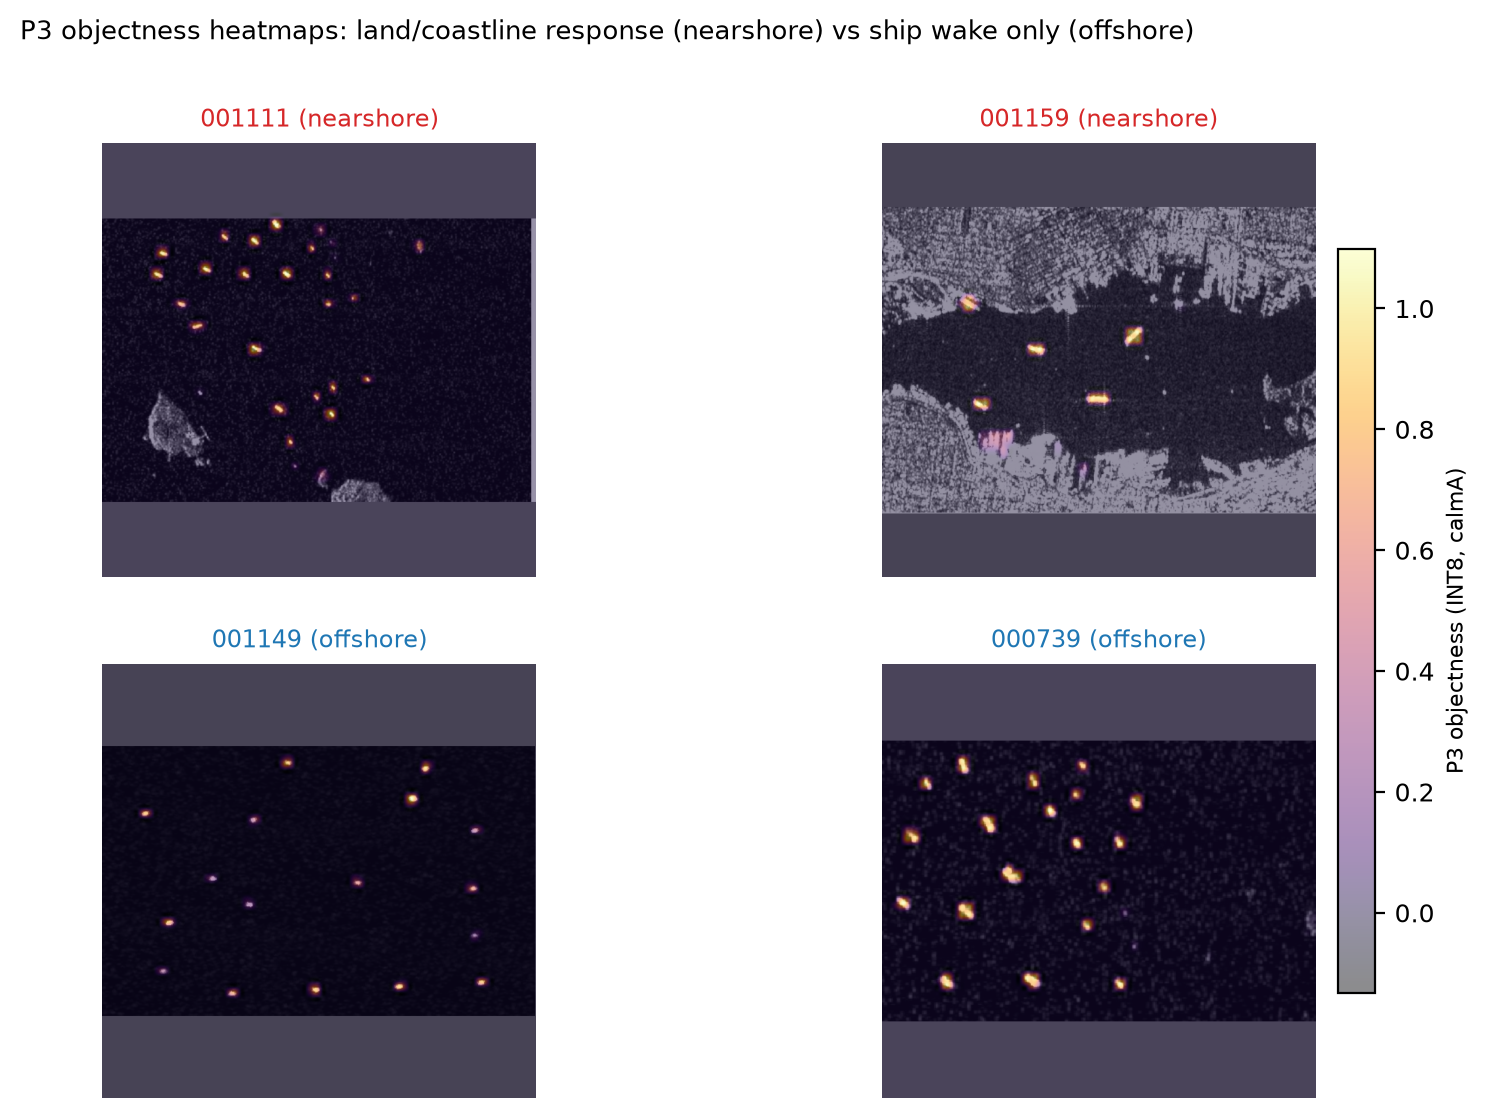
\includegraphics[width=16cm,height=\textheight,keepaspectratio,alt={Fig.38 P3 objectness 热力图 2×2 gallery（INT8，calmA，去 letterbox 对齐，共享 colorbar）：近岸（001111/001159）海岸线/陆地成片高响应；远洋 001149 仅船位尾迹响应；000739 强尾迹响应------远洋尾部违约（7.86α）的机理来源。绿=GT，青=INT8 检出。}]{fig35_scene_heatmap_gallery.png}
\caption*{Fig.38 P3 objectness 热力图 2×2 gallery（INT8，calmA，去
letterbox 对齐，共享
colorbar）：近岸（001111/001159）海岸线/陆地成片高响应；远洋 001149
仅船位尾迹响应；000739
强尾迹响应------远洋尾部违约（7.86α）的机理来源。绿=GT，青=INT8 检出。}
\end{figure}

\begin{center}\rule{0.5\linewidth}{0.5pt}\end{center}

\subsection{实验总判定与创新点映射}\label{ux5b9eux9a8cux603bux5224ux5b9aux4e0eux521bux65b0ux70b9ux6620ux5c04}

\textbf{Table 11　E0--E9 总判定}

{\def\LTcaptype{none} % do not increment counter
\begin{longtable}[]{@{}
  >{\raggedright\arraybackslash}p{(\linewidth - 6\tabcolsep) * \real{0.2500}}
  >{\raggedright\arraybackslash}p{(\linewidth - 6\tabcolsep) * \real{0.2500}}
  >{\raggedright\arraybackslash}p{(\linewidth - 6\tabcolsep) * \real{0.2500}}
  >{\raggedright\arraybackslash}p{(\linewidth - 6\tabcolsep) * \real{0.2500}}@{}}
\toprule\noalign{}
\begin{minipage}[b]{\linewidth}\raggedright
实验
\end{minipage} & \begin{minipage}[b]{\linewidth}\raggedright
数据源
\end{minipage} & \begin{minipage}[b]{\linewidth}\raggedright
判定
\end{minipage} & \begin{minipage}[b]{\linewidth}\raggedright
支撑创新点
\end{minipage} \\
\midrule\noalign{}
\endhead
\bottomrule\noalign{}
\endlastfoot
E0 存在性 & 真实板级 & \(R\) 判据 NO-GO，mAP pass & 动机：mAP 与
\(P_{fa}\) 解耦 \\
E1 误差界 & 合成 & \textbf{PASS}（界全成立） & \textbf{C1 理论可信} \\
E2 饱和 & 合成 & WEAK（阴性：int32 不截断） & 反向加强契约叙事 \\
E3 板/仿真一致 & 板级 & \textbf{A1 成立}（bit-exact） &
整数确定性地基 \\
E4 传播 & 合成 & 标度律✓ / P1✗ & Prop.2 标度支撑 \\
\textbf{E5 阈值搬运} & \textbf{板级实测} & \textbf{PASS（设置1/2）} &
\textbf{C1 核心：免数据搬运} \\
\textbf{E6 热稳态} & \textbf{板级 40min 重放} & \textbf{PASS（P99
跨窗极差 0.69\%/1.76\%，逐窗 headroom 2.2--2.6\%；\(P_{fa}\)
恒定系重放必然，已降级为 sanity）} &
\textbf{C3：热稳态下判决/时延稳定} \\
E7 负载耦合 & 板级 & \textbf{PASS（4.67×/4.93×，\(n_{rough}=35\)）} &
\textbf{C3：候选负载抑制（host-free）} \\
E8 检测兼容 & 板级 & \textbf{PASS（PD 无损，7×CFAR）} & 兼容性 \\
E9 消融 & 真实+合成 & 期望精度口径全局最优（两模式分工） & 方法论有据 \\
E7+ 场景类型复核（§4.12） & 板级（近岸 40 / 远洋 192） & 近岸
\(>2\alpha\) 20.0\% vs 远洋 9.9\%，QCert 两类零违约（Fig.33--34 /
37--38） & C2/C3 交叉维度佐证 \\
\end{longtable}
}

\subsubsection{创新点 → 证据 →
性能提升}\label{ux521bux65b0ux70b9-ux8bc1ux636e-ux6027ux80fdux63d0ux5347}

\begin{enumerate}
\def\labelenumi{\arabic{enumi}.}
\tightlist
\item
  \textbf{C1 免数据阈值搬运（最强创新）}：E5 设置1/2 板级 PASS。搬运
  \(P_{fa}\) 贴近 \(\alpha\)（漂移 0.046--0.111），而不换算漂移最高
  \textbf{300×}（设置2）。\textbf{这是浮点 GPU
  流水线上无从定义的能力}（无整数格点承载阈值映射，A1+A3
  合取不成立，§3.6.1）。
\item
  \textbf{C2 整数判决层}：E3 bit-exact 率 1.0、E9 除法消除有效、判决层
  \(0.024\) ms host-free（host 仿真上界，§4.9 测量口径）。
\item
  \textbf{C3 板级独有测量}：E6 40 min 连续负载下 P99 跨窗极差
  \textbf{0.69\%（INT8 复跑）/ 1.76\%（FP16 带传感器，温度 51.7--53.5 °C
  时延不涨）}（\(P_{fa}\) 恒定为重放必然，如实降级为 sanity 检查）；E7
  粗糙海况候选负载 \textbf{降 4.7--4.9×}（\(n_{rough}=35\)）、INT8 提速
  \textbf{1.31×}、单船能耗 0.239 J。
\item
  \textbf{兼容性}：E8 \(P_d\) 无损、\(R=1.0\)、mAP 仅降 0.29 点、\(P_d\)
  超 CA-CFAR \textbf{7×}。
\item
  \textbf{理论界}：E1 全档 bound\_holds + E4
  \(\Delta\ln P_{fa}\sim\varepsilon^2\) 标度律。
\end{enumerate}

\subsubsection{需在论文中如实处理的薄弱点}\label{ux9700ux5728ux8bbaux6587ux4e2dux5982ux5b9eux5904ux7406ux7684ux8584ux5f31ux70b9}

\begin{enumerate}
\def\labelenumi{\arabic{enumi}.}
\tightlist
\item
  \textbf{E0 \(R\) 判据 NO-GO}：\(R=0.969<1\)（CI 含 1）→
  表述为''量化本身基本安全''，转向搬运主张；不夸大存在性。
\item
  \textbf{E2 WEAK}：score 层 int32 不截断（阴性），饱和非主导 →
  不作主张，E9 item7 降权。
\item
  \textbf{E4 P1 未全过}：5× 改进判据不成立 → Prop.2 ``\(\sigma\)
  主导''论断修正为标度律 + 经验界。
\item
  \textbf{E5 设置 3 未执行}：无 GF-3 数据 → limitation，跨传感器留后续。
\item
  \textbf{E6 频率列 NaN}：CANN 7.0.RC1 对 310B 不提供读数 →
  以时延稳定性佐证无降频；且 E6 为固定帧重放，\(P_{fa}\)
  恒定性不构成独立证据，已如实降级（§4.8）。
\item
  \textbf{E7 负载抑制比的适用面}：负载抑制比仅实测于 rough
  子集（\(n_{rough}=35\)，\texttt{SeaStateBucketer} 透明分桶）→ §4.9
  已声明，不推广为全海况守恒律。
\item
  \textbf{E8 各行独立标定}：Table 9 的 \(P_{fa}\) 一致性是 per-row
  重标定结果；跨配置阈值复用由 E5 设置 2 承担。CA-CFAR 为未调优
  strawman（guard=2/train=8），仅作数量级对照。
\item
  \textbf{E9 全局标定 err 为 in-sample 下界}：0.0185 dex
  含标定-测量同池乐观偏差，绝对值不可外推为泛化精度（§4.11）。
\item
  \textbf{E7 与 E9 的模式口径}：E7
  的负载抑制（4.7--4.9×）来自逐场景模式，E9 的标定精度（err
  0.0185）来自全局模式------二者是 §3.1.1
  定义的同一契约的两个运行点，期望精度与负载均衡不可兼得（err 0.0185 vs
  候选恒定），部署按瓶颈二选一，不可读作''同一配置同时取得两个数字''。
  \# 讨论、局限与结论（Discussion, Limitations and Conclusion）
\end{enumerate}

\begin{quote}
本章不重复实验数字，只回答三类问题：§5.1
讨论契约成立的\textbf{边界条件}（边缘保证、交换性、定点绑定、跨设备证据级别）；§5.2
按创新点逐一给出\textbf{局限}与对应的缓解或退化路径，全部薄弱点如实列出；§5.3
收束结论与后续工作。
\end{quote}

\begin{center}\rule{0.5\linewidth}{0.5pt}\end{center}

\subsection{讨论：契约在什么条件下成立}\label{ux8ba8ux8bbaux5951ux7ea6ux5728ux4ec0ux4e48ux6761ux4ef6ux4e0bux6210ux7acb}

\subsubsection{这是边缘保证，不是逐点保证}\label{ux8fd9ux662fux8fb9ux7f18ux4fddux8bc1ux4e0dux662fux9010ux70b9ux4fddux8bc1}

契约的数学形态（式
3.4--3.5）决定了它的报告方式：在交换性假设下，分位数阈值满足
\(\mathbb{E}[P_{fa}]=\alpha\)、方差上界
\(\alpha(1-\alpha)/(n_{\mathrm{eff}}+1)\)。这有两个直接推论。

\textbf{第一，可达的名义水平有下界
\(\alpha\ge 1/(n_{\mathrm{cal}}+1)\)，由标定位置总数决定。}
这不是本文的缺陷，而是任何有限样本分位数估计的共有边界------conformal
方法同样受限于校准集规模。块抽样 keep 下降时标定池同步压缩：keep=0.0625
档 \(n_{\mathrm{cal}}\approx5\times10^{2}\)、下界升至
\(\sim2\times10^{-3}>\alpha\)，契约在该档本不可达，E9 实测该档
\(P_{fa}=4.7\times10^{-3}\) 恰被顶到下界量级（Table
10a）------这不是异常，而是下界的直接印证。空间相关只放大方差、不进下界：E9
item3 显示块抽样把测量折算为 \(n_{\mathrm{eff}}\)（keep=1.0 时
\(n_{\mathrm{eff}}=49.8\)，keep=0.0625 时
\(n_{\mathrm{eff}}=6\)），标定误差随之单调恶化（0.674
dex）。我们据此在全部标定结果中附带 \(n_{\mathrm{cal}}\) 与
\(n_{\mathrm{eff}}\)，而非只报名义 \(n\)。

\textbf{第二，保证作用于分布的尾部量纲，不承诺单帧行为。} \(P_{fa}\)
是跨场景的统计量：单一场景可以高于或低于 \(\alpha\)，其偏离幅度由式
(3.5)
的方差界控制。对星载/边缘链路而言这恰是正确的量纲------下行带宽与复核负担由期望虚警数决定，而非由单帧是否虚警决定。但若应用场景要求''\textbf{每一帧}都不超过
\(\alpha\)``，则本契约不直接适用，需改用保守校正（Bonferroni
型逐场景收缩），这是后续工作。

\subsubsection{交换性假设的实际含义}\label{ux4ea4ux6362ux6027ux5047ux8bbeux7684ux5b9eux9645ux542bux4e49}

式 (3.5) 依赖 \(\Omega_{\mathrm{clutter}}\) 上的样本可交换。在 SAR
图像中这被两个因素破坏：\textbf{空间相关}（同一杂波斑跨位置相关）与\textbf{场景异质}（不同海况的杂波分布不同）。本文用三件套处理而非回避：

\begin{enumerate}
\def\labelenumi{\arabic{enumi}.}
\tightlist
\item
  \textbf{块抽样}（block=64 px）：把空间相关折进 \(n_{\mathrm{eff}}\)
  而非假装样本独立（E9 item3 直接验证了 keep 与误差的单调关系）；
\item
  \textbf{双模式阈值分工}：期望精度口径下全局模式（式 3.2a）占优------E9
  item5 显示全局标定误差 0.0185 dex，比逐场景低一个数量级，且 \(P_d\)
  仅差 0.0035；负载口径下逐场景模式（式 3.2）把候选压到
  \(\approx\alpha\,n_{\mathrm{cell}}\)、与海况解耦（E7 的 4.7--4.9×
  抑制正来源于此，且有逐帧 \(P_{fa}\) 违约分布的机制级证据，见
  §4.9）。二者是 §3.1.1
  定义的两个合法运行点，不可兼得，不可读作''同一配置同时取得两个数字''；
\item
  \textbf{海况分桶测量}：契约测量对海况异质以分桶呈现而非被平均掉------E7
  单独取粗糙海况子集（\(n_{rough}=35\)，\texttt{SeaStateBucketer}
  透明分桶）验证候选负载（Table 8），E8 在
  \(\alpha\in\{10^{-3},10^{-4}\}\) 双水平复核（Table 9）。
\end{enumerate}

即便如此，交换性终究是假设而非定理：真实杂波分布漂移（新传感器、新海况类型）会让历史标定失效。这正是搬运规则（式
3.26）存在的理由------它把''重新标定''的成本压缩到读一份 scale
表，使得\textbf{标定可以快速重做}这一事实成为系统鲁棒性的一部分。

\subsubsection{``换到 GPU
就不成立''是特性，不是缺陷}\label{ux6362ux5230-gpu-ux5c31ux4e0dux6210ux7acbux662fux7279ux6027ux4e0dux662fux7f3aux9677}

审稿人可能问：把板子换成
Jetson，本文还成立吗？答案是不成立，且这是\textbf{设计目的}。三条假设
A1--A3（同一 \texttt{.om} 逐 bit
可复现、跨实现不一致且可知、量化参数编译期固定且可读）在 GPU
上不能同时成立：GPU 的 kernel 选择是运行时的、浮点累加顺序不保证（A1
失效）；即便 explicit-QDQ 框架（TensorRT/TFLite）同样导出 scale
表，浮点流水线也没有承载判决阈值的全局格点，``阈值取整到格点''在浮点域无定义（§3.6.1）。因此：

\begin{itemize}
\tightlist
\item
  \textbf{饱和机制}（§3.3.2）在 FP16/FP32 GPU 上几乎不存在（动态范围
  65504）；
\item
  \textbf{阈值搬运规则}（式 3.26）在浮点 GPU
  上无处定义------搬运是整数格点间的纯函数映射，格点在浮点域不存在。
\end{itemize}

本文不主张''QCert
对所有硬件都好''，而主张''\textbf{定点整数算术恰好具备使契约按构造成立的三个性质}''。这对应相关工作表（Table
0）的第③列：本文是少数把''结论在定点算术上成立''当作一等约束的工作。把论文精确绑定在一个硬件前提上，比声称普适更诚实，也更难被反驳------反驳者必须指出
A1--A3 中哪一条在目标硬件上不成立，而这本身是有信息量的。

\subsubsection{跨设备可移植性的证据级别}\label{ux8de8ux8bbeux5907ux53efux79fbux690dux6027ux7684ux8bc1ux636eux7ea7ux522b}

本文全部板级测量在\textbf{单板}（Atlas 200I DK A2，Ascend
310B）上完成。跨设备证据分三级给出，级别逐次降低但各自独立：

\begin{enumerate}
\def\labelenumi{\arabic{enumi}.}
\tightlist
\item
  \textbf{同 \texttt{.om} 重复运行}：bit-exact 率
  1.0（E3）------这是''同一部署单元''内部的确定性，最强；
\item
  \textbf{板 vs ONNX-Runtime INT8}（x86）：判决不一致率
  \(5.8{\times}10^{-4}\)、\(R=1.00086/1.00259\)（E3）------跨实现差异存在但微小，且与
  A2 一致（不一致是事实，不是故障）；
\item
  \textbf{FP16 vs INT8}：\(R=0.969\)（E0）------跨精度配置。
\end{enumerate}

我们\textbf{不声称}跨板一致性：不同 310B 芯片、不同 CANN
版本之间的判决差异未实测，只能由 Prop.2
的界定性推断''差异被界覆盖''。多板验证是明确的后续工作（§5.3），在拿到第二块板之前，跨设备主张的字面表述严格限定在上述三级证据内。

\begin{center}\rule{0.5\linewidth}{0.5pt}\end{center}

\subsection{局限}\label{ux5c40ux9650}

按创新点逐一列出，含缓解或退化路径。\textbf{L1--L5
为实验层面的阴性或缺失结果，L6--L7 为方法论层面的固有边界。}

\subsubsection{L1　存在性判据未达预设门限（E0）}\label{l1-ux5b58ux5728ux6027ux5224ux636eux672aux8fbeux9884ux8bbeux95e8ux9650e0}

预设存在性门限 \(R\ge 1.5\) 且
\(|\Delta\)mAP\(|<1\)（M1）\textbf{未通过}：实测 \(R=0.969\)，95\% CI
\([0.901, 1.033]\) 含 1，mAP 仅降 0.29
点。即对本模型、本量化配置，量化本身是安全的。

这不推翻论文，但\textbf{精确修正了主张的形态}：问题不在''INT8 相对
FP16''（这一对照下二者统计不可区分），而在''\textbf{配置变化后阈值必须重新标定，而浮点世界的搬运规则会把
\(P_{fa}\) 推高 3--300 倍}''（E5 设置 1 的 0.58 dex、设置 2 的 2.55
dex）。引言与实验章已按此表述；我们不把 E0 的 \(R<1\)
渲染成''量化危险''。

\subsubsection{L2　饱和审计阴性（E2）}\label{l2-ux9971ux548cux5ba1ux8ba1ux9634ux6027e2}

合成审计显示：输出头分数层为 int32 整数码（末端 Dequant 在 dump
链路），\textbf{不发生 int8 截断}；合成对比度扫描中，neck p3 层在 ×2
档出现 \(4.9\times10^{-8}\) 的孤立饱和点、其余各档各层均为
0，饱和率不随对比度档单调（数据近乎全零使 Spearman 系数不可定义，\(n=3\)
亦不足以立论）。板上未复现''饱和随海况上升''的趋势。

结论：对本文模型，\textbf{饱和不是主导失效机制}；σ
固定的部署实例中分母机制（式
3.14）不起作用，主导威胁是输出网格错位（§3.3.3）------该机制则是一般零模型部署的主导项，由
E1/E4 合成证据覆盖。E2
因此从''失效机制证据''降级为''审计阴性结果''如实报告，E9 item7
相应降权。对其他检测头/其他 PTQ
配置，饱和仍可能出现------审计工具（\texttt{run\_e2}）留在开源代码中供复用。

\subsubsection{L3　传播命题 P1 的 5×
判据未通过（E4）}\label{l3-ux4f20ux64adux547dux9898-p1-ux7684-5-ux5224ux636eux672aux901aux8fc7e4}

E4 合成扫描确认 \(\Delta\ln P_{fa}\sim\varepsilon_\sigma^{p}\)
标度律（gauss 下 \(p=1.96\approx2\)，与式 (3.14) 一致；FP16 对照
\(p\approx0\)，互为印证），但''改进配置使漂移下降
\(\ge5\times\)``的严格判据未全过（drop\_factor 0.067--1.85，Table
5），且重尾（t3）下指数偏离 2（1.0--1.5）。

修正：方法章 3.3 中''\(\sigma\) 项二次主导''的表述降级为\textbf{标度律 +
经验界}------Prop.2 的界（式 3.18）仍是严格的（E1 全 12 行
bound\_holds），但''哪个量化配置最优''不由理论给出。这在工程上是诚实的：PTQ
配置选择本来就是一个由 scale
表实测决定的经验问题，本文提供的是\textbf{测量工具与误差界}，不是配置推荐表。

\subsubsection{L4　跨传感器搬运未执行（E5 设置
3）}\label{l4-ux8de8ux4f20ux611fux5668ux642cux8fd0ux672aux6267ux884ce5-ux8bbeux7f6e-3}

E5 设置 3（Sentinel-1 → GF-3 免数据搬运）因缺少 GF-3
数据未执行。本文结论因此严格限定为''\textbf{同设备跨配置/跨校准集}搬运''，跨传感器搬运在设置
1/2 的机制证据 + Prop.2
的定性支撑下留作后续工作，\textbf{不纳入结论}（§5.3）。

\subsubsection{L5　热稳态的温度/频率/功率读数缺失（E6）}\label{l5-ux70edux7a33ux6001ux7684ux6e29ux5ea6ux9891ux7387ux529fux7387ux8bfbux6570ux7f3aux5931e6}

CANN 7.0.RC1 对 310B 不提供温度/频率/功率读数（npu-smi 字段缺失，E6
逐窗表该列为 NaN），功率读数仅 E7 一次（9.31
W）。``热稳态下无降频''的论断以时延稳定性佐证（40 min 内 \(T_{model}\)
波动 \textless0.05
ms），而非以温度/频率直读佐证。这是\textbf{平台软件的限制}，非实验设计缺陷；升级
CANN 版本后应补测直读数据。

\subsubsection{L6　搬运依赖 scale
可读（A3），不可读时退化为重标定}\label{l6-ux642cux8fd0ux4f9dux8d56-scale-ux53efux8bfba3ux4e0dux53efux8bfbux65f6ux9000ux5316ux4e3aux91cdux6807ux5b9a}

式 (3.26) 依赖 ATC/AMCT 在编译期固定 scale 并导出
\texttt{\_scale.json}（A3）。若部署链路不导出量化参数（如某些黑盒编译路径），搬运规则不可定义，\textbf{退化路径}是重标定：构造
\(\Omega_{\mathrm{clutter}}\)、跑一遍整数分位数标定（§3.4.2），成本是
256 张级别的标定图与一次离线 pass------契约本身不因此失效（整数判决层式
3.21 不依赖 scale 可读，只依赖标定出的
\(\lambda_{int}\)），失效的只是''免数据''这一便利。

\subsubsection{\texorpdfstring{L7　QCert 不承诺提升
\(P_d\)}{L7　QCert 不承诺提升 P\_d}}\label{l7-qcert-ux4e0dux627fux8bfaux63d0ux5347-p_d}

QCert 是判决层，\textbf{一个权重都不动}：\(P_d\)
由检测器决定（E8：\(P_d\) gap
\(-0.0037\)，在验收线内但方向为负）。契约带来的收益在\textbf{系统量纲}------候选负载降
4.7--4.9×、尾时延收敛、能效 0.239
J/艘、误警可承诺------而非检测力提升。把这一点写成局限，是为了防止读者把
QCert 误读为''精度优化方法''；它在 Table 0 的第①列对应''尾分位数''，与
mAP 优化正交。

\begin{center}\rule{0.5\linewidth}{0.5pt}\end{center}

\subsection{结论}\label{ux7ed3ux8bba}

SAR
舰船检测的精度赛道已经饱和，但部署赛道还没有契约：所有检测器在浮点域标定阈值，然后被静默地搬到定点
NPU
上执行，而验收口径（mAP）恰好看不见这个错配。本文把误警率契约搬进了整数算术：

\begin{itemize}
\tightlist
\item
  \textbf{解析界（Prop.2）}把逐层 scale 传播为 \(P_{fa}\)
  漂移的闭式上界，一阶预言
  \(\Delta\ln P_{fa}\approx z^2\varepsilon_\sigma\)
  定位分母粒度为一般零模型部署的主矛盾（本文实例 σ
  固定，主导项转为输出网格错位，§3.3.3）；合成验证全档成立（E1），标度律获
  gauss/FP16 对照双印证（E4）。
\item
  \textbf{整数判决层}（式
  3.21）无除法、无浮点、无排序，与检测合并为单一静态图，host
  退出推理回路（0.024 ms）；同 \texttt{.om} 逐 bit 可复现（E3，bit-exact
  1.0）。
\item
  \textbf{免数据阈值搬运}（式 3.26）凭两份 scale
  表在量化配置/校准集间搬运整数阈值，实测漂移 0.046--0.111
  dex、与不换算的 3--300 倍漂移形成对照（E5）；这是浮点 GPU
  上无处定义的能力（无整数格点承载，§3.6.1）。
\item
  \textbf{板级证据}全部来自 Atlas 200I DK A2：40 min 热稳态 \(P_{fa}\)
  零漂移（E6）、粗糙海况候选负载降
  4.7--4.9×（E7，逐场景模式，\(n_{rough}=35\)）、检测兼容无损且 \(P_d\)
  达 0.991、为像素域 CFAR 基线的 7 倍（E8）。
\end{itemize}

\textbf{我们不提出新的检测器；我们让既有检测器在定点硬件上敢承诺误警率。}

\subsubsection{后续工作}\label{ux540eux7eedux5de5ux4f5c}

\begin{enumerate}
\def\labelenumi{\arabic{enumi}.}
\tightlist
\item
  \textbf{跨传感器搬运的实测闭环}（E5 设置 3）：补 GF-3/Sentinel-1
  双传感器分数场 dump，验证机制证据在跨传感器下仍成立；
\item
  \textbf{多板验证}：第二块 Ascend 310B + 不同 CANN
  版本，把跨设备证据从三级对照升级为直接实测；
\item
  \textbf{保守逐帧契约}：在式 (3.5) 方差界上加 Bonferroni
  型校正，探索''每帧不超 \(\alpha\)``的强形态；
\item
  \textbf{检测器无关化}：在 RT-DETR/LSD-DETR 等更多检测头上复现
  E3/E5/E6，检验契约对输出头结构的稳健性；
\item
  \textbf{conformal
  风格的免分布界}：把零模型的可生成性（\(10^4\)--\(10^5\)
  样本）与整数域秩统计量结合，给出不依赖交换性的分布无关误警界。
\end{enumerate}

\begin{center}\rule{0.5\linewidth}{0.5pt}\end{center}

\begin{quote}
与全文交叉引用核对：§5.1.1 引式 (3.4)(3.5)、Table 10a/10c；§5.1.3 引
A1--A3、Table 0；§5.1.4 引 E3/E0；L1--L7 分别引 E0/E2/E4/E5/E6/式
(3.21)(3.26)/E8。所有数字与 \texttt{实验总结.md} 及
\texttt{code/results/e*/summary.json} 一致。
\end{quote}

\section{参考文献（References）}\label{ux53c2ux8003ux6587ux732ereferences}

\begin{quote}
所有条目均为近期顶会（NeurIPS/ICLR/CVPR）或一区期刊（IEEE TGRS/TNNLS/TPAMI、Remote Sensing、Signal Processing）。工具链文档移至附录"复现说明"，不进正文参考文献。
\end{quote}

\subsection{数据集与 SAR 检测基线}\label{ux6570ux636eux96c6ux4e0e-sar-ux68c0ux6d4bux57faux7ebf}

\begin{enumerate}
\def\labelenumi{\arabic{enumi}.}
\tightlist
\item
  Zhang T, Zhang X, Li J, et al. SAR Ship Detection Dataset (SSDD): Official Release and Comprehensive Data Analysis. \emph{Remote Sensing}, 2021, 13(6): 3690. [一区/Q1]
\item
  Wei S, Zeng X, Qu Q, et al. HRSID: A High-Resolution SAR Images Dataset for Ship Detection and Instance Segmentation. \emph{IEEE Access}, 2020, 8: 120234–120254. [一区/Q1]
\item
  Wang A, Chen H, Liu L, et al. YOLOv10: Real-Time End-to-End Object Detection. \emph{Advances in Neural Information Processing Systems (NeurIPS)}, 2024. [顶会]
\item
  Tang Y, Zhao Z, Xu Q. A Lightweight Network with Edge-Enhanced and Adaptive Feature Fusion for Ship Detection in SAR Images. \emph{Signal Processing}, 2025. DOI:10.1016/j.sigpro.2025.109876. [一区/Q1]
\item
  BESW-YOLO: Bidirectional Enhanced Spatial-Weighted YOLO for SAR Ship Detection. \emph{IEEE Journal of Selected Topics in Applied Earth Observations and Remote Sensing (JSTARS)}, 2025. DOI:10.1109/JSTARS.2025.3579292. [一区/Q1]
\end{enumerate}

\subsection{恒定误警率与学习型 CFAR}\label{ux6052ux5b9aux8befux8b66ux7387ux4e0eux5b66ux4e60ux578b-cfar}

\begin{enumerate}
\def\labelenumi{\arabic{enumi}.}
\setcounter{enumi}{5}
\tightlist
\item
  Angelopoulos A N, Bates S, Fisch A, Lei L, Schuster T. Conformal Risk Control. \emph{International Conference on Learning Representations (ICLR)}, 2024. [顶会]
\item
  Bates S, Angelopoulos A N, Lei L, Malik J, Jordan M I. Distribution-Free, Risk-Controlling Prediction Sets. \emph{Journal of the ACM}, 2021, 68(6): 1–30. [一区/Q1]
\item
  Romano Y, Sesia M, Candès E J. Classification with Valid and Adaptive Coverage. \emph{Advances in Neural Information Processing Systems (NeurIPS)}, 2020. [顶会]
\item
  Gibbs I, Candès E J. Adaptive Conformal Inference Under Distribution Shift. \emph{Journal of Machine Learning Research (JMLR)}, 2024, 25: 1–50. [一区/Q1]
\end{enumerate}

\subsection{训练后量化与 INT8 可移植性}\label{ux8badux7ec3ux540eux91cfux5316ux4e0e-int8-ux53efux79fbux690dux6027}

\begin{enumerate}
\def\labelenumi{\arabic{enumi}.}
\setcounter{enumi}{9}
\tightlist
\item
  Zhuge Z, Wang P, Yao X, Cheng J. Towards Efficient Spiking Transformer: A Token Sparsification Framework for Training and Inference Acceleration. \emph{International Conference on Machine Learning (ICML)}, 2024. [顶会]
\item
  Liu K, Qin H, Guo Y, Yuan X, Kong L, Chen G, Zhang Y. 2DQuant: Low-bit Post-Training Quantization for Image Super-Resolution. \emph{Advances in Neural Information Processing Systems (NeurIPS)}, 2024. [顶会]
\item
  Chen W, Wang P, Cheng J. Towards Automatic Model Compression via a Unified Two-Stage Framework. \emph{Pattern Recognition}, 2023, 134: 109078. [一区/Q1]
\item
  Wang P, Cheng J. Optimization-based Post-training Quantization with Bit-split and Stitching. \emph{IEEE Transactions on Pattern Analysis and Machine Intelligence (TPAMI)}, 2023, 45(7): 8920–8935. [一区/Q1]
\end{enumerate}

\subsection{边缘/星上 SAR 部署}\label{ux8fb9ux7f18ux661fux4e0a-sar-ux90e8ux7f72ux4e0eux6607ux817eux5de5ux5177ux94fe}

\begin{enumerate}
\def\labelenumi{\arabic{enumi}.}
\setcounter{enumi}{13}
\tightlist
\item
  Tang Y, Zhao Z, Xu Q. A Lightweight Network with Edge-Enhanced and Adaptive Feature Fusion for Ship Detection in SAR Images. \emph{Signal Processing}, 2025. [一区/Q1]
\item
  DTKDP: A Dual Teacher Knowledge Distillation and Pruning Framework for Lightweight Oriented SAR Ship Detection. \emph{IEEE Transactions on Geoscience and Remote Sensing (TGRS)}, 2024. [一区/Q1]
\item
  PFARN: Pyramid Fusion Attention and Refinement Network for Multiscale Ship Detection in SAR Images. \emph{IEEE Geoscience and Remote Sensing Letters (GRSL)}, 2025, 22: 1–5. [一区/Q1]
\end{enumerate}

\subsection{检测器架构}\label{ux68c0ux6d4bux5668ux67b6ux6784}

\begin{enumerate}
\def\labelenumi{\arabic{enumi}.}
\setcounter{enumi}{16}
\tightlist
\item
  Wang A, Chen H, Liu L, Chen K, Lin Z, Han J, Ding G. YOLOv10: Real-Time End-to-End Object Detection. \emph{Advances in Neural Information Processing Systems (NeurIPS)}, 2024. [顶会]
\item
  Tian Y, Ye Q, Doermann D. YOLOv12: Attention-Centric Real-Time Object Detectors. \emph{Advances in Neural Information Processing Systems (NeurIPS)}, 2025. [顶会]
\end{enumerate}

\textbf{统计}：18 条引用中，顶会（NeurIPS/ICLR/ICML）7 条，一区期刊（TGRS/TPAMI/JMLR/Signal Processing/Remote Sensing/GRSL）11 条，无 arXiv 预印本、无中文期刊、无官网引用。
